\documentclass[twoside]{book}

% Packages required by doxygen
\usepackage{fixltx2e}
\usepackage{calc}
\usepackage{doxygen}
\usepackage{graphicx}
\usepackage[utf8]{inputenc}
\usepackage{makeidx}
\usepackage{multicol}
\usepackage{multirow}
\PassOptionsToPackage{warn}{textcomp}
\usepackage{textcomp}
\usepackage[nointegrals]{wasysym}
\usepackage[table]{xcolor}

% NLS support packages
\usepackage[italian]{babel}

% Font selection
\usepackage[T1]{fontenc}
\usepackage{mathptmx}
\usepackage[scaled=.90]{helvet}
\usepackage{courier}
\usepackage{amssymb}
\usepackage{sectsty}
\renewcommand{\familydefault}{\sfdefault}
\allsectionsfont{%
  \fontseries{bc}\selectfont%
  \color{darkgray}%
}
\renewcommand{\DoxyLabelFont}{%
  \fontseries{bc}\selectfont%
  \color{darkgray}%
}
\newcommand{\+}{\discretionary{\mbox{\scriptsize$\hookleftarrow$}}{}{}}

% Page & text layout
\usepackage{geometry}
\geometry{%
  a4paper,%
  top=2.5cm,%
  bottom=2.5cm,%
  left=2.5cm,%
  right=2.5cm%
}
\tolerance=750
\hfuzz=15pt
\hbadness=750
\setlength{\emergencystretch}{15pt}
\setlength{\parindent}{0cm}
\setlength{\parskip}{0.2cm}
\makeatletter
\renewcommand{\paragraph}{%
  \@startsection{paragraph}{4}{0ex}{-1.0ex}{1.0ex}{%
    \normalfont\normalsize\bfseries\SS@parafont%
  }%
}
\renewcommand{\subparagraph}{%
  \@startsection{subparagraph}{5}{0ex}{-1.0ex}{1.0ex}{%
    \normalfont\normalsize\bfseries\SS@subparafont%
  }%
}
\makeatother

% Headers & footers
\usepackage{fancyhdr}
\pagestyle{fancyplain}
\fancyhead[LE]{\fancyplain{}{\bfseries\thepage}}
\fancyhead[CE]{\fancyplain{}{}}
\fancyhead[RE]{\fancyplain{}{\bfseries\leftmark}}
\fancyhead[LO]{\fancyplain{}{\bfseries\rightmark}}
\fancyhead[CO]{\fancyplain{}{}}
\fancyhead[RO]{\fancyplain{}{\bfseries\thepage}}
\fancyfoot[LE]{\fancyplain{}{}}
\fancyfoot[CE]{\fancyplain{}{}}
\fancyfoot[RE]{\fancyplain{}{\bfseries\scriptsize Generato Sab 10 Giu 2017 00\+:29\+:30 per Zynq-\/7000 Driver Pack da Doxygen }}
\fancyfoot[LO]{\fancyplain{}{\bfseries\scriptsize Generato Sab 10 Giu 2017 00\+:29\+:30 per Zynq-\/7000 Driver Pack da Doxygen }}
\fancyfoot[CO]{\fancyplain{}{}}
\fancyfoot[RO]{\fancyplain{}{}}
\renewcommand{\footrulewidth}{0.4pt}
\renewcommand{\chaptermark}[1]{%
  \markboth{#1}{}%
}
\renewcommand{\sectionmark}[1]{%
  \markright{\thesection\ #1}%
}

% Indices & bibliography
\usepackage{natbib}
\usepackage[titles]{tocloft}
\setcounter{tocdepth}{3}
\setcounter{secnumdepth}{5}
\makeindex

% Hyperlinks (required, but should be loaded last)
\usepackage{ifpdf}
\ifpdf
  \usepackage[pdftex,pagebackref=true]{hyperref}
\else
  \usepackage[ps2pdf,pagebackref=true]{hyperref}
\fi
\hypersetup{%
  colorlinks=true,%
  linkcolor=blue,%
  citecolor=blue,%
  unicode%
}

% Custom commands
\newcommand{\clearemptydoublepage}{%
  \newpage{\pagestyle{empty}\cleardoublepage}%
}


%===== C O N T E N T S =====

\begin{document}

% Titlepage & ToC
\hypersetup{pageanchor=false,
             bookmarks=true,
             bookmarksnumbered=true,
             pdfencoding=unicode
            }
\pagenumbering{roman}
\begin{titlepage}
\vspace*{7cm}
\begin{center}%
{\Large Zynq-\/7000 Driver Pack \\[1ex]\large 2.\+0 }\\
\vspace*{1cm}
{\large Generato da Doxygen 1.8.8}\\
\vspace*{0.5cm}
{\small Sab 10 Giu 2017 00:29:30}\\
\end{center}
\end{titlepage}
\clearemptydoublepage
\tableofcontents
\clearemptydoublepage
\pagenumbering{arabic}
\hypersetup{pageanchor=true}

%--- Begin generated contents ---
\chapter{Indice dei moduli}
\section{Moduli}
Questo è l'elenco di tutti i moduli\+:\begin{DoxyCompactList}
\item \contentsline{section}{L\+C\+D}{\pageref{group___l_c_d}}{}
\begin{DoxyCompactList}
\item \contentsline{section}{H\+D44780}{\pageref{group___h_d44780}}{}
\end{DoxyCompactList}
\item \contentsline{section}{Zybo}{\pageref{group___zybo}}{}
\begin{DoxyCompactList}
\item \contentsline{section}{Button}{\pageref{group___button}}{}
\item \contentsline{section}{Led}{\pageref{group___led}}{}
\item \contentsline{section}{Switch}{\pageref{group___switch}}{}
\end{DoxyCompactList}
\item \contentsline{section}{G\+P\+I\+O}{\pageref{group___g_p_i_o}}{}
\end{DoxyCompactList}

\chapter{Indice delle strutture dati}
\section{Strutture dati}
Queste sono le strutture dati con una loro breve descrizione\+:\begin{DoxyCompactList}
\item\contentsline{section}{\hyperlink{struct_g_p_i_o__t}{G\+P\+I\+O\+\_\+t} \\*Struttura che astrae un device G\+P\+I\+O }{\pageref{struct_g_p_i_o__t}}{}
\item\contentsline{section}{\hyperlink{struct_h_d44780___l_c_d__t}{H\+D44780\+\_\+\+L\+C\+D\+\_\+t} \\*Struttura opaca che astrae un device Display L\+C\+D con cntroller Hitachi H\+D44780, o compatibile. Un oggetto di tipo \hyperlink{struct_h_d44780___l_c_d__t}{H\+D44780\+\_\+\+L\+C\+D\+\_\+t} rappresenta un device lcd H\+D44780. Il modulo e' pensato per permettere la gestione di piu' display da parte dello stesso processore, agendo su oggetti \hyperlink{struct_h_d44780___l_c_d__t}{H\+D44780\+\_\+\+L\+C\+D\+\_\+t} diversi. Il modulo permette di utilizzare sia l'interfacciamento ad otto bit che quello a quattro bit, inizializzando il device opportunamente, attraverso l'uso delle funzioni H\+D44780\+\_\+\+Init8 e\+H\+D44780\+\_\+\+Init4. Il modulo fornisce anche semplici funzioni per la stampa di un carattere o di una stringa null-\/terminated di caratteri. Si veda la documentazione delle funzioni H\+D44780\+\_\+\+Printc e H\+D44780\+\_\+\+Print. Inoltre sono presenti diverse funzioni di utilita' generica, come quelle per la pulizia del display, per lo spostamento del cursore di un posto in avanti o indietro, alla riga in basso o in alto }{\pageref{struct_h_d44780___l_c_d__t}}{}
\item\contentsline{section}{\hyperlink{struct_zybo_button__t}{Zybo\+Button\+\_\+t} \\*Struttura opaca che astrae l'insieme dei button presenti sulla board Digilent Zybo; }{\pageref{struct_zybo_button__t}}{}
\item\contentsline{section}{\hyperlink{struct_zybo_led__t}{Zybo\+Led\+\_\+t} \\*Struttura opaca che astrae l'insieme dei Led presenti sulla board Digilent Zybo; }{\pageref{struct_zybo_led__t}}{}
\item\contentsline{section}{\hyperlink{struct_zybo_switch__t}{Zybo\+Switch\+\_\+t} \\*Struttura opaca che astrae l'insieme degli switch presenti sulla board Digilent Zybo; }{\pageref{struct_zybo_switch__t}}{}
\end{DoxyCompactList}

\chapter{Indice dei file}
\section{Elenco dei file}
Questo è un elenco di tutti i file con una loro breve descrizione\+:\begin{DoxyCompactList}
\item\contentsline{section}{G\+P\+I\+O/\hyperlink{my_g_p_i_o_8c}{my\+G\+P\+I\+O.\+c} }{\pageref{my_g_p_i_o_8c}}{}
\item\contentsline{section}{G\+P\+I\+O/\hyperlink{my_g_p_i_o_8h}{my\+G\+P\+I\+O.\+h} }{\pageref{my_g_p_i_o_8h}}{}
\item\contentsline{section}{Lcd/\hyperlink{hd44780_8c}{hd44780.\+c} }{\pageref{hd44780_8c}}{}
\item\contentsline{section}{Lcd/\hyperlink{hd44780_8h}{hd44780.\+h} }{\pageref{hd44780_8h}}{}
\item\contentsline{section}{Zybo/\hyperlink{_zybo_8h}{Zybo.\+h} }{\pageref{_zybo_8h}}{}
\item\contentsline{section}{Zybo/\hyperlink{_zybo_button_8c}{Zybo\+Button.\+c} }{\pageref{_zybo_button_8c}}{}
\item\contentsline{section}{Zybo/\hyperlink{_zybo_button_8h}{Zybo\+Button.\+h} }{\pageref{_zybo_button_8h}}{}
\item\contentsline{section}{Zybo/\hyperlink{_zybo_led_8c}{Zybo\+Led.\+c} }{\pageref{_zybo_led_8c}}{}
\item\contentsline{section}{Zybo/\hyperlink{_zybo_led_8h}{Zybo\+Led.\+h} }{\pageref{_zybo_led_8h}}{}
\item\contentsline{section}{Zybo/\hyperlink{_zybo_switch_8c}{Zybo\+Switch.\+c} }{\pageref{_zybo_switch_8c}}{}
\item\contentsline{section}{Zybo/\hyperlink{_zybo_switch_8h}{Zybo\+Switch.\+h} }{\pageref{_zybo_switch_8h}}{}
\end{DoxyCompactList}

\chapter{Documentazione dei moduli}
\hypertarget{group___l_c_d}{\section{L\+C\+D}
\label{group___l_c_d}\index{L\+C\+D@{L\+C\+D}}
}
\subsection*{Strutture dati}
\begin{DoxyCompactItemize}
\item 
struct \hyperlink{struct_h_d44780___l_c_d__t}{H\+D44780\+\_\+\+L\+C\+D\+\_\+t}
\begin{DoxyCompactList}\small\item\em Struttura opaca che astrae un device Display L\+C\+D con cntroller Hitachi H\+D44780, o compatibile. Un oggetto di tipo \hyperlink{struct_h_d44780___l_c_d__t}{H\+D44780\+\_\+\+L\+C\+D\+\_\+t} rappresenta un device lcd H\+D44780. Il modulo e' pensato per permettere la gestione di piu' display da parte dello stesso processore, agendo su oggetti \hyperlink{struct_h_d44780___l_c_d__t}{H\+D44780\+\_\+\+L\+C\+D\+\_\+t} diversi. Il modulo permette di utilizzare sia l'interfacciamento ad otto bit che quello a quattro bit, inizializzando il device opportunamente, attraverso l'uso delle funzioni H\+D44780\+\_\+\+Init8 e\+H\+D44780\+\_\+\+Init4. Il modulo fornisce anche semplici funzioni per la stampa di un carattere o di una stringa null-\/terminated di caratteri. Si veda la documentazione delle funzioni H\+D44780\+\_\+\+Printc e H\+D44780\+\_\+\+Print. Inoltre sono presenti diverse funzioni di utilita' generica, come quelle per la pulizia del display, per lo spostamento del cursore di un posto in avanti o indietro, alla riga in basso o in alto. \end{DoxyCompactList}\end{DoxyCompactItemize}
\subsection*{Tipi enumerati (enum)}
\begin{DoxyCompactItemize}
\item 
enum \hyperlink{group___l_c_d_gaaaea8b73e24f7658da4118f6b01b45f0}{H\+D44780\+\_\+\+Interface\+Mode\+\_\+t} \{ \hyperlink{group___l_c_d_ggaaaea8b73e24f7658da4118f6b01b45f0a45bf6ce7ec7c951f692bdce9f0f485c6}{H\+D44780\+\_\+\+I\+N\+T\+E\+R\+F\+A\+C\+E\+\_\+4bit}, 
\hyperlink{group___l_c_d_ggaaaea8b73e24f7658da4118f6b01b45f0a24da9b234f9358c14184fe21f3c47de5}{H\+D44780\+\_\+\+I\+N\+T\+E\+R\+F\+A\+C\+E\+\_\+8bit}
 \}
\item 
enum \hyperlink{group___l_c_d_gaf46f4db4f981d3a1088804a6d6980d30}{H\+D44780\+\_\+\+Direction\+\_\+t} \{ \hyperlink{group___l_c_d_ggaf46f4db4f981d3a1088804a6d6980d30aa4d704398d4edd1e0dec8dbb55f90292}{H\+D44780\+\_\+\+Cursor\+Left}, 
\hyperlink{group___l_c_d_ggaf46f4db4f981d3a1088804a6d6980d30a26006ced693b6bab28c6e30bfdb8c399}{H\+D44780\+\_\+\+Cursor\+Right}
 \}
\begin{DoxyCompactList}\small\item\em Direzioni di spostamento del cursore. \end{DoxyCompactList}\end{DoxyCompactItemize}
\subsection*{Funzioni}
\begin{DoxyCompactItemize}
\item 
void \hyperlink{group___l_c_d_ga2df14171c71a8afda59e3ae1733c5469}{H\+D44780\+\_\+\+Init8} (\hyperlink{struct_h_d44780___l_c_d__t}{H\+D44780\+\_\+\+L\+C\+D\+\_\+t} $\ast$lcd, \hyperlink{struct_g_p_i_o__t}{G\+P\+I\+O\+\_\+t} $\ast$gpio, \hyperlink{group___g_p_i_o_ga6d5aef8a8a54ee2f602d47252ff66595}{G\+P\+I\+O\+\_\+mask} R\+S, \hyperlink{group___g_p_i_o_ga6d5aef8a8a54ee2f602d47252ff66595}{G\+P\+I\+O\+\_\+mask} R\+W, \hyperlink{group___g_p_i_o_ga6d5aef8a8a54ee2f602d47252ff66595}{G\+P\+I\+O\+\_\+mask} E, \hyperlink{group___g_p_i_o_ga6d5aef8a8a54ee2f602d47252ff66595}{G\+P\+I\+O\+\_\+mask} Data7, \hyperlink{group___g_p_i_o_ga6d5aef8a8a54ee2f602d47252ff66595}{G\+P\+I\+O\+\_\+mask} Data6, \hyperlink{group___g_p_i_o_ga6d5aef8a8a54ee2f602d47252ff66595}{G\+P\+I\+O\+\_\+mask} Data5, \hyperlink{group___g_p_i_o_ga6d5aef8a8a54ee2f602d47252ff66595}{G\+P\+I\+O\+\_\+mask} Data4, \hyperlink{group___g_p_i_o_ga6d5aef8a8a54ee2f602d47252ff66595}{G\+P\+I\+O\+\_\+mask} Data3, \hyperlink{group___g_p_i_o_ga6d5aef8a8a54ee2f602d47252ff66595}{G\+P\+I\+O\+\_\+mask} Data2, \hyperlink{group___g_p_i_o_ga6d5aef8a8a54ee2f602d47252ff66595}{G\+P\+I\+O\+\_\+mask} Data1, \hyperlink{group___g_p_i_o_ga6d5aef8a8a54ee2f602d47252ff66595}{G\+P\+I\+O\+\_\+mask} Data0)
\begin{DoxyCompactList}\small\item\em Inizializza un display lcd H\+D44780 con interfacciamento ad 8 bit. \end{DoxyCompactList}\item 
void \hyperlink{group___l_c_d_gad8f777df204bc630b77924e0a96e5673}{H\+D44780\+\_\+\+Init4} (\hyperlink{struct_h_d44780___l_c_d__t}{H\+D44780\+\_\+\+L\+C\+D\+\_\+t} $\ast$lcd, \hyperlink{struct_g_p_i_o__t}{G\+P\+I\+O\+\_\+t} $\ast$gpio, \hyperlink{group___g_p_i_o_ga6d5aef8a8a54ee2f602d47252ff66595}{G\+P\+I\+O\+\_\+mask} R\+S, \hyperlink{group___g_p_i_o_ga6d5aef8a8a54ee2f602d47252ff66595}{G\+P\+I\+O\+\_\+mask} R\+W, \hyperlink{group___g_p_i_o_ga6d5aef8a8a54ee2f602d47252ff66595}{G\+P\+I\+O\+\_\+mask} E, \hyperlink{group___g_p_i_o_ga6d5aef8a8a54ee2f602d47252ff66595}{G\+P\+I\+O\+\_\+mask} Data7, \hyperlink{group___g_p_i_o_ga6d5aef8a8a54ee2f602d47252ff66595}{G\+P\+I\+O\+\_\+mask} Data6, \hyperlink{group___g_p_i_o_ga6d5aef8a8a54ee2f602d47252ff66595}{G\+P\+I\+O\+\_\+mask} Data5, \hyperlink{group___g_p_i_o_ga6d5aef8a8a54ee2f602d47252ff66595}{G\+P\+I\+O\+\_\+mask} Data4)
\begin{DoxyCompactList}\small\item\em Inizializza un oggetto display lcd H\+D44780 affinche' si utilizzi l'interfaccia a 4 bit. \end{DoxyCompactList}\item 
void \hyperlink{group___l_c_d_ga57b8c6ca0b3c12e5f7273b3c373a6f17}{H\+D44780\+\_\+\+Printc} (\hyperlink{struct_h_d44780___l_c_d__t}{H\+D44780\+\_\+\+L\+C\+D\+\_\+t} $\ast$lcd, char c)
\begin{DoxyCompactList}\small\item\em Stampa un carattere. \end{DoxyCompactList}\item 
void \hyperlink{group___l_c_d_ga3aedff8e2040e62db569fde955d3987b}{H\+D44780\+\_\+\+Print} (\hyperlink{struct_h_d44780___l_c_d__t}{H\+D44780\+\_\+\+L\+C\+D\+\_\+t} $\ast$lcd, const char $\ast$s)
\begin{DoxyCompactList}\small\item\em Stampa una stringa null-\/terminated di caratteri. \end{DoxyCompactList}\item 
void \hyperlink{group___l_c_d_ga38cac13d7a66f068be54f79a716ff7d4}{H\+D44780\+\_\+\+Clear} (\hyperlink{struct_h_d44780___l_c_d__t}{H\+D44780\+\_\+\+L\+C\+D\+\_\+t} $\ast$lcd)
\begin{DoxyCompactList}\small\item\em Pulisce il display e sposta il cursore all'inizio della prima riga. \end{DoxyCompactList}\item 
void \hyperlink{group___l_c_d_ga68e3712332aa9482d4bdaa4991a92127}{H\+D44780\+\_\+\+Home} (\hyperlink{struct_h_d44780___l_c_d__t}{H\+D44780\+\_\+\+L\+C\+D\+\_\+t} $\ast$lcd)
\begin{DoxyCompactList}\small\item\em Sposta il cursore all'inizio della prima riga. \end{DoxyCompactList}\item 
void \hyperlink{group___l_c_d_gad90e2924a4e632ce42940323f8f49e37}{H\+D44780\+\_\+\+Move\+To\+Row1} (\hyperlink{struct_h_d44780___l_c_d__t}{H\+D44780\+\_\+\+L\+C\+D\+\_\+t} $\ast$lcd)
\begin{DoxyCompactList}\small\item\em Sposta il cursore all'inizio della prima riga. \end{DoxyCompactList}\item 
void \hyperlink{group___l_c_d_ga713670d498b6f5d50a174df19081c515}{H\+D44780\+\_\+\+Move\+To\+Row2} (\hyperlink{struct_h_d44780___l_c_d__t}{H\+D44780\+\_\+\+L\+C\+D\+\_\+t} $\ast$lcd)
\begin{DoxyCompactList}\small\item\em Sposta il cursore all'inizio della seconda riga. \end{DoxyCompactList}\item 
void \hyperlink{group___l_c_d_gabcea9a03050c46530e39b7556c673baf}{H\+D44780\+\_\+\+Move\+Cursor} (\hyperlink{struct_h_d44780___l_c_d__t}{H\+D44780\+\_\+\+L\+C\+D\+\_\+t} $\ast$lcd, \hyperlink{group___l_c_d_gaf46f4db4f981d3a1088804a6d6980d30}{H\+D44780\+\_\+\+Direction\+\_\+t} dir)
\begin{DoxyCompactList}\small\item\em Sposta il cursore di una posizione a destra o sinistra. \end{DoxyCompactList}\item 
void \hyperlink{group___l_c_d_ga5cf07b2179272029410f9a81f56621ed}{H\+D44780\+\_\+\+Display\+Off} (\hyperlink{struct_h_d44780___l_c_d__t}{H\+D44780\+\_\+\+L\+C\+D\+\_\+t} $\ast$lcd)
\begin{DoxyCompactList}\small\item\em Disattiva il display. \end{DoxyCompactList}\item 
void \hyperlink{group___l_c_d_ga56421dc398825188aa10257063a3ee4b}{H\+D44780\+\_\+\+Cursor\+Off} (\hyperlink{struct_h_d44780___l_c_d__t}{H\+D44780\+\_\+\+L\+C\+D\+\_\+t} $\ast$lcd)
\begin{DoxyCompactList}\small\item\em Disattiva la visualizzazione del cursore. \end{DoxyCompactList}\item 
void \hyperlink{group___l_c_d_ga3a381cb44df5d76d79be5ed71a52bae6}{H\+D44780\+\_\+\+Cursor\+On} (\hyperlink{struct_h_d44780___l_c_d__t}{H\+D44780\+\_\+\+L\+C\+D\+\_\+t} $\ast$lcd)
\begin{DoxyCompactList}\small\item\em Attiva la visualizzazione del cursore. \end{DoxyCompactList}\item 
void \hyperlink{group___l_c_d_ga92eb58cb7d73c9a87b7087a9c56f73d5}{H\+D44780\+\_\+\+Cursor\+Blink} (\hyperlink{struct_h_d44780___l_c_d__t}{H\+D44780\+\_\+\+L\+C\+D\+\_\+t} $\ast$lcd)
\begin{DoxyCompactList}\small\item\em Attiva il cursore lampeggiante. \end{DoxyCompactList}\end{DoxyCompactItemize}


\subsection{Descrizione dettagliata}


\subsection{Documentazione dei tipi enumerati}
\hypertarget{group___l_c_d_gaf46f4db4f981d3a1088804a6d6980d30}{\index{L\+C\+D@{L\+C\+D}!H\+D44780\+\_\+\+Direction\+\_\+t@{H\+D44780\+\_\+\+Direction\+\_\+t}}
\index{H\+D44780\+\_\+\+Direction\+\_\+t@{H\+D44780\+\_\+\+Direction\+\_\+t}!L\+C\+D@{L\+C\+D}}
\subsubsection[{H\+D44780\+\_\+\+Direction\+\_\+t}]{\setlength{\rightskip}{0pt plus 5cm}enum {\bf H\+D44780\+\_\+\+Direction\+\_\+t}}}\label{group___l_c_d_gaf46f4db4f981d3a1088804a6d6980d30}


Direzioni di spostamento del cursore. 

\begin{Desc}
\item[Valori del tipo enumerato]\par
\begin{description}
\index{H\+D44780\+\_\+\+Cursor\+Left@{H\+D44780\+\_\+\+Cursor\+Left}!L\+C\+D@{L\+C\+D}}\index{L\+C\+D@{L\+C\+D}!H\+D44780\+\_\+\+Cursor\+Left@{H\+D44780\+\_\+\+Cursor\+Left}}\item[{\em 
\hypertarget{group___l_c_d_ggaf46f4db4f981d3a1088804a6d6980d30aa4d704398d4edd1e0dec8dbb55f90292}{H\+D44780\+\_\+\+Cursor\+Left}\label{group___l_c_d_ggaf46f4db4f981d3a1088804a6d6980d30aa4d704398d4edd1e0dec8dbb55f90292}
}]left sposta il cursore a sinistra \index{H\+D44780\+\_\+\+Cursor\+Right@{H\+D44780\+\_\+\+Cursor\+Right}!L\+C\+D@{L\+C\+D}}\index{L\+C\+D@{L\+C\+D}!H\+D44780\+\_\+\+Cursor\+Right@{H\+D44780\+\_\+\+Cursor\+Right}}\item[{\em 
\hypertarget{group___l_c_d_ggaf46f4db4f981d3a1088804a6d6980d30a26006ced693b6bab28c6e30bfdb8c399}{H\+D44780\+\_\+\+Cursor\+Right}\label{group___l_c_d_ggaf46f4db4f981d3a1088804a6d6980d30a26006ced693b6bab28c6e30bfdb8c399}
}]right sposta il cursore a destra \end{description}
\end{Desc}
\hypertarget{group___l_c_d_gaaaea8b73e24f7658da4118f6b01b45f0}{\index{L\+C\+D@{L\+C\+D}!H\+D44780\+\_\+\+Interface\+Mode\+\_\+t@{H\+D44780\+\_\+\+Interface\+Mode\+\_\+t}}
\index{H\+D44780\+\_\+\+Interface\+Mode\+\_\+t@{H\+D44780\+\_\+\+Interface\+Mode\+\_\+t}!L\+C\+D@{L\+C\+D}}
\subsubsection[{H\+D44780\+\_\+\+Interface\+Mode\+\_\+t}]{\setlength{\rightskip}{0pt plus 5cm}enum {\bf H\+D44780\+\_\+\+Interface\+Mode\+\_\+t}}}\label{group___l_c_d_gaaaea8b73e24f7658da4118f6b01b45f0}
\begin{Desc}
\item[Valori del tipo enumerato]\par
\begin{description}
\index{H\+D44780\+\_\+\+I\+N\+T\+E\+R\+F\+A\+C\+E\+\_\+4bit@{H\+D44780\+\_\+\+I\+N\+T\+E\+R\+F\+A\+C\+E\+\_\+4bit}!L\+C\+D@{L\+C\+D}}\index{L\+C\+D@{L\+C\+D}!H\+D44780\+\_\+\+I\+N\+T\+E\+R\+F\+A\+C\+E\+\_\+4bit@{H\+D44780\+\_\+\+I\+N\+T\+E\+R\+F\+A\+C\+E\+\_\+4bit}}\item[{\em 
\hypertarget{group___l_c_d_ggaaaea8b73e24f7658da4118f6b01b45f0a45bf6ce7ec7c951f692bdce9f0f485c6}{H\+D44780\+\_\+\+I\+N\+T\+E\+R\+F\+A\+C\+E\+\_\+4bit}\label{group___l_c_d_ggaaaea8b73e24f7658da4118f6b01b45f0a45bf6ce7ec7c951f692bdce9f0f485c6}
}]\index{H\+D44780\+\_\+\+I\+N\+T\+E\+R\+F\+A\+C\+E\+\_\+8bit@{H\+D44780\+\_\+\+I\+N\+T\+E\+R\+F\+A\+C\+E\+\_\+8bit}!L\+C\+D@{L\+C\+D}}\index{L\+C\+D@{L\+C\+D}!H\+D44780\+\_\+\+I\+N\+T\+E\+R\+F\+A\+C\+E\+\_\+8bit@{H\+D44780\+\_\+\+I\+N\+T\+E\+R\+F\+A\+C\+E\+\_\+8bit}}\item[{\em 
\hypertarget{group___l_c_d_ggaaaea8b73e24f7658da4118f6b01b45f0a24da9b234f9358c14184fe21f3c47de5}{H\+D44780\+\_\+\+I\+N\+T\+E\+R\+F\+A\+C\+E\+\_\+8bit}\label{group___l_c_d_ggaaaea8b73e24f7658da4118f6b01b45f0a24da9b234f9358c14184fe21f3c47de5}
}]\end{description}
\end{Desc}


\subsection{Documentazione delle funzioni}
\hypertarget{group___l_c_d_ga38cac13d7a66f068be54f79a716ff7d4}{\index{L\+C\+D@{L\+C\+D}!H\+D44780\+\_\+\+Clear@{H\+D44780\+\_\+\+Clear}}
\index{H\+D44780\+\_\+\+Clear@{H\+D44780\+\_\+\+Clear}!L\+C\+D@{L\+C\+D}}
\subsubsection[{H\+D44780\+\_\+\+Clear}]{\setlength{\rightskip}{0pt plus 5cm}void H\+D44780\+\_\+\+Clear (
\begin{DoxyParamCaption}
\item[{{\bf H\+D44780\+\_\+\+L\+C\+D\+\_\+t} $\ast$}]{lcd}
\end{DoxyParamCaption}
)}}\label{group___l_c_d_ga38cac13d7a66f068be54f79a716ff7d4}


Pulisce il display e sposta il cursore all'inizio della prima riga. 


\begin{DoxyParams}{Parametri}
{\em lcd} & display da pilotare; \\
\hline
\end{DoxyParams}
\hypertarget{group___l_c_d_ga92eb58cb7d73c9a87b7087a9c56f73d5}{\index{L\+C\+D@{L\+C\+D}!H\+D44780\+\_\+\+Cursor\+Blink@{H\+D44780\+\_\+\+Cursor\+Blink}}
\index{H\+D44780\+\_\+\+Cursor\+Blink@{H\+D44780\+\_\+\+Cursor\+Blink}!L\+C\+D@{L\+C\+D}}
\subsubsection[{H\+D44780\+\_\+\+Cursor\+Blink}]{\setlength{\rightskip}{0pt plus 5cm}void H\+D44780\+\_\+\+Cursor\+Blink (
\begin{DoxyParamCaption}
\item[{{\bf H\+D44780\+\_\+\+L\+C\+D\+\_\+t} $\ast$}]{lcd}
\end{DoxyParamCaption}
)}}\label{group___l_c_d_ga92eb58cb7d73c9a87b7087a9c56f73d5}


Attiva il cursore lampeggiante. 


\begin{DoxyParams}{Parametri}
{\em lcd} & display da pilotare; \\
\hline
\end{DoxyParams}
\hypertarget{group___l_c_d_ga56421dc398825188aa10257063a3ee4b}{\index{L\+C\+D@{L\+C\+D}!H\+D44780\+\_\+\+Cursor\+Off@{H\+D44780\+\_\+\+Cursor\+Off}}
\index{H\+D44780\+\_\+\+Cursor\+Off@{H\+D44780\+\_\+\+Cursor\+Off}!L\+C\+D@{L\+C\+D}}
\subsubsection[{H\+D44780\+\_\+\+Cursor\+Off}]{\setlength{\rightskip}{0pt plus 5cm}void H\+D44780\+\_\+\+Cursor\+Off (
\begin{DoxyParamCaption}
\item[{{\bf H\+D44780\+\_\+\+L\+C\+D\+\_\+t} $\ast$}]{lcd}
\end{DoxyParamCaption}
)}}\label{group___l_c_d_ga56421dc398825188aa10257063a3ee4b}


Disattiva la visualizzazione del cursore. 


\begin{DoxyParams}{Parametri}
{\em lcd} & display da pilotare; \\
\hline
\end{DoxyParams}
\hypertarget{group___l_c_d_ga3a381cb44df5d76d79be5ed71a52bae6}{\index{L\+C\+D@{L\+C\+D}!H\+D44780\+\_\+\+Cursor\+On@{H\+D44780\+\_\+\+Cursor\+On}}
\index{H\+D44780\+\_\+\+Cursor\+On@{H\+D44780\+\_\+\+Cursor\+On}!L\+C\+D@{L\+C\+D}}
\subsubsection[{H\+D44780\+\_\+\+Cursor\+On}]{\setlength{\rightskip}{0pt plus 5cm}void H\+D44780\+\_\+\+Cursor\+On (
\begin{DoxyParamCaption}
\item[{{\bf H\+D44780\+\_\+\+L\+C\+D\+\_\+t} $\ast$}]{lcd}
\end{DoxyParamCaption}
)}}\label{group___l_c_d_ga3a381cb44df5d76d79be5ed71a52bae6}


Attiva la visualizzazione del cursore. 


\begin{DoxyParams}{Parametri}
{\em lcd} & display da pilotare; \\
\hline
\end{DoxyParams}
\hypertarget{group___l_c_d_ga5cf07b2179272029410f9a81f56621ed}{\index{L\+C\+D@{L\+C\+D}!H\+D44780\+\_\+\+Display\+Off@{H\+D44780\+\_\+\+Display\+Off}}
\index{H\+D44780\+\_\+\+Display\+Off@{H\+D44780\+\_\+\+Display\+Off}!L\+C\+D@{L\+C\+D}}
\subsubsection[{H\+D44780\+\_\+\+Display\+Off}]{\setlength{\rightskip}{0pt plus 5cm}void H\+D44780\+\_\+\+Display\+Off (
\begin{DoxyParamCaption}
\item[{{\bf H\+D44780\+\_\+\+L\+C\+D\+\_\+t} $\ast$}]{lcd}
\end{DoxyParamCaption}
)}}\label{group___l_c_d_ga5cf07b2179272029410f9a81f56621ed}


Disattiva il display. 


\begin{DoxyParams}{Parametri}
{\em lcd} & display da pilotare; \\
\hline
\end{DoxyParams}
\hypertarget{group___l_c_d_ga68e3712332aa9482d4bdaa4991a92127}{\index{L\+C\+D@{L\+C\+D}!H\+D44780\+\_\+\+Home@{H\+D44780\+\_\+\+Home}}
\index{H\+D44780\+\_\+\+Home@{H\+D44780\+\_\+\+Home}!L\+C\+D@{L\+C\+D}}
\subsubsection[{H\+D44780\+\_\+\+Home}]{\setlength{\rightskip}{0pt plus 5cm}void H\+D44780\+\_\+\+Home (
\begin{DoxyParamCaption}
\item[{{\bf H\+D44780\+\_\+\+L\+C\+D\+\_\+t} $\ast$}]{lcd}
\end{DoxyParamCaption}
)}}\label{group___l_c_d_ga68e3712332aa9482d4bdaa4991a92127}


Sposta il cursore all'inizio della prima riga. 


\begin{DoxyParams}{Parametri}
{\em lcd} & display da pilotare; \\
\hline
\end{DoxyParams}
\hypertarget{group___l_c_d_gad8f777df204bc630b77924e0a96e5673}{\index{L\+C\+D@{L\+C\+D}!H\+D44780\+\_\+\+Init4@{H\+D44780\+\_\+\+Init4}}
\index{H\+D44780\+\_\+\+Init4@{H\+D44780\+\_\+\+Init4}!L\+C\+D@{L\+C\+D}}
\subsubsection[{H\+D44780\+\_\+\+Init4}]{\setlength{\rightskip}{0pt plus 5cm}void H\+D44780\+\_\+\+Init4 (
\begin{DoxyParamCaption}
\item[{{\bf H\+D44780\+\_\+\+L\+C\+D\+\_\+t} $\ast$}]{lcd, }
\item[{{\bf G\+P\+I\+O\+\_\+t} $\ast$}]{gpio, }
\item[{{\bf G\+P\+I\+O\+\_\+mask}}]{R\+S, }
\item[{{\bf G\+P\+I\+O\+\_\+mask}}]{R\+W, }
\item[{{\bf G\+P\+I\+O\+\_\+mask}}]{E, }
\item[{{\bf G\+P\+I\+O\+\_\+mask}}]{Data7, }
\item[{{\bf G\+P\+I\+O\+\_\+mask}}]{Data6, }
\item[{{\bf G\+P\+I\+O\+\_\+mask}}]{Data5, }
\item[{{\bf G\+P\+I\+O\+\_\+mask}}]{Data4}
\end{DoxyParamCaption}
)}}\label{group___l_c_d_gad8f777df204bc630b77924e0a96e5673}


Inizializza un oggetto display lcd H\+D44780 affinche' si utilizzi l'interfaccia a 4 bit. 

Inizializza un oggetto \hyperlink{struct_h_d44780___l_c_d__t}{H\+D44780\+\_\+\+L\+C\+D\+\_\+t} verificando la validita' delle coppie porta-\/pin per l' interfacciamento, configurando i pin G\+P\+I\+O e inizializzando il device.

\begin{DoxyWarning}{Avvertimento}
Se i pin associati ai segnali di pilotaggio del device non sono correttamente configurati come pin di output, il dispositivo non funzionera' correttamente.

Non modificare i campi della struttura \hyperlink{struct_h_d44780___l_c_d__t}{H\+D44780\+\_\+\+L\+C\+D\+\_\+t} dopo che essa sia stata inizializzata.

La struttura \hyperlink{struct_g_p_i_o__t}{G\+P\+I\+O\+\_\+t}, a cui fa riferimento il parametro gpio, va inizializzata a parte.
\end{DoxyWarning}

\begin{DoxyParams}{Parametri}
{\em lcd} & puntatore a struttura di tipo \hyperlink{struct_h_d44780___l_c_d__t}{H\+D44780\+\_\+\+L\+C\+D\+\_\+t} che descrive un display H\+D44780 da inizializzare; \\
\hline
{\em gpio} & puntatore alla struttura \hyperlink{struct_g_p_i_o__t}{G\+P\+I\+O\+\_\+t} che astrae il device G\+P\+I\+O a cui il display e' connesso. Non viene inizializzato dalla funziona, sara' necessario inizializzarlo preventivamente; \\
\hline
{\em R\+S} & pin del device G\+P\+I\+O a cui e' associato il segnale R\+S (data/command) del display L\+C\+D; \\
\hline
{\em R\+W} & pin del device G\+P\+I\+O a cui e' associato il segnale R\+W (read/write) del display L\+C\+D; \\
\hline
{\em E} & pin del device G\+P\+I\+O a cui e' associato il segnale E (Enable) del display L\+C\+D; \\
\hline
{\em Data7} & pin del device G\+P\+I\+O a cui e' associato il segnale Data7 del display L\+C\+D; \\
\hline
{\em Data6} & pin del device G\+P\+I\+O a cui e' associato il segnale Data6 del display L\+C\+D; \\
\hline
{\em Data5} & pin del device G\+P\+I\+O a cui e' associato il segnale Data5 del display L\+C\+D; \\
\hline
{\em Data4} & pin del device G\+P\+I\+O a cui e' associato il segnale Data4 del display L\+C\+D;\\
\hline
\end{DoxyParams}

\begin{DoxyCode}
1 GPIO\_t gpioDisplay;
2 GPIO\_init(&gpioDisplay, XPAR\_MYGPIO\_3\_S00\_AXI\_BASEADDR, 11, 0, 4, 8);
3 HD44780\_LCD\_t lcd;
4 HD44780\_Init4(&lcd, &gpioDisplay,   GPIO\_pin10, GPIO\_pin9, GPIO\_pin8,
5                                         GPIO\_pin0, GPIO\_pin1, GPIO\_pin2, GPIO\_pin3);
6 HD44780\_Print(&lcd, "Ciao! Come va");
7 HD44780\_MoveToRow2(&lcd);
8 HD44780\_Print(&lcd, "lo studio?");
\end{DoxyCode}
 \hypertarget{group___l_c_d_ga2df14171c71a8afda59e3ae1733c5469}{\index{L\+C\+D@{L\+C\+D}!H\+D44780\+\_\+\+Init8@{H\+D44780\+\_\+\+Init8}}
\index{H\+D44780\+\_\+\+Init8@{H\+D44780\+\_\+\+Init8}!L\+C\+D@{L\+C\+D}}
\subsubsection[{H\+D44780\+\_\+\+Init8}]{\setlength{\rightskip}{0pt plus 5cm}void H\+D44780\+\_\+\+Init8 (
\begin{DoxyParamCaption}
\item[{{\bf H\+D44780\+\_\+\+L\+C\+D\+\_\+t} $\ast$}]{lcd, }
\item[{{\bf G\+P\+I\+O\+\_\+t} $\ast$}]{gpio, }
\item[{{\bf G\+P\+I\+O\+\_\+mask}}]{R\+S, }
\item[{{\bf G\+P\+I\+O\+\_\+mask}}]{R\+W, }
\item[{{\bf G\+P\+I\+O\+\_\+mask}}]{E, }
\item[{{\bf G\+P\+I\+O\+\_\+mask}}]{Data7, }
\item[{{\bf G\+P\+I\+O\+\_\+mask}}]{Data6, }
\item[{{\bf G\+P\+I\+O\+\_\+mask}}]{Data5, }
\item[{{\bf G\+P\+I\+O\+\_\+mask}}]{Data4, }
\item[{{\bf G\+P\+I\+O\+\_\+mask}}]{Data3, }
\item[{{\bf G\+P\+I\+O\+\_\+mask}}]{Data2, }
\item[{{\bf G\+P\+I\+O\+\_\+mask}}]{Data1, }
\item[{{\bf G\+P\+I\+O\+\_\+mask}}]{Data0}
\end{DoxyParamCaption}
)}}\label{group___l_c_d_ga2df14171c71a8afda59e3ae1733c5469}


Inizializza un display lcd H\+D44780 con interfacciamento ad 8 bit. 

\begin{DoxyWarning}{Avvertimento}
Se i pin associati ai segnali di pilotaggio del device non sono correttamente configurati come pin di output, il dispositivo non funzionera' correttamente.

Non modificare i campi della struttura dopo che essa sia stata inizializzata.

La struttura \hyperlink{struct_g_p_i_o__t}{G\+P\+I\+O\+\_\+t}, a cui fa riferimento il parametro gpio, va inizializzata a parte.
\end{DoxyWarning}

\begin{DoxyParams}{Parametri}
{\em lcd} & puntatore a struttura di tipo \hyperlink{struct_h_d44780___l_c_d__t}{H\+D44780\+\_\+\+L\+C\+D\+\_\+t} che descrive un display H\+D44780 da inizializzare; \\
\hline
{\em gpio} & puntatore alla struttura \hyperlink{struct_g_p_i_o__t}{G\+P\+I\+O\+\_\+t} che astrae il device G\+P\+I\+O a cui il display e' connesso. Non viene inizializzato dalla funziona, sara' necessario inizializzarlo preventivamente; \\
\hline
{\em R\+S} & pin del device G\+P\+I\+O a cui e' associato il segnale R\+S (data/command) del display L\+C\+D; \\
\hline
{\em R\+W} & pin del device G\+P\+I\+O a cui e' associato il segnale R\+W (read/write) del display L\+C\+D; \\
\hline
{\em E} & pin del device G\+P\+I\+O a cui e' associato il segnale E (Enable) del display L\+C\+D; \\
\hline
{\em Data7} & pin del device G\+P\+I\+O a cui e' associato il segnale Data7 del display L\+C\+D; \\
\hline
{\em Data6} & pin del device G\+P\+I\+O a cui e' associato il segnale Data6 del display L\+C\+D; \\
\hline
{\em Data5} & pin del device G\+P\+I\+O a cui e' associato il segnale Data5 del display L\+C\+D; \\
\hline
{\em Data4} & pin del device G\+P\+I\+O a cui e' associato il segnale Data4 del display L\+C\+D; \\
\hline
{\em Data3} & pin del device G\+P\+I\+O a cui e' associato il segnale Data3 del display L\+C\+D; \\
\hline
{\em Data2} & pin del device G\+P\+I\+O a cui e' associato il segnale Data2 del display L\+C\+D; \\
\hline
{\em Data1} & pin del device G\+P\+I\+O a cui e' associato il segnale Data1 del display L\+C\+D; \\
\hline
{\em Data0} & pin del device G\+P\+I\+O a cui e' associato il segnale Data0 del display L\+C\+D;\\
\hline
\end{DoxyParams}

\begin{DoxyCode}
1 GPIO\_t gpioDisplay;
2 GPIO\_init(&gpioDisplay, XPAR\_MYGPIO\_3\_S00\_AXI\_BASEADDR, 11, 0, 4, 8);
3 HD44780\_LCD\_t lcd;
4 HD44780\_Init8(&lcd, &gpioDisplay,   GPIO\_pin10, GPIO\_pin9, GPIO\_pin8,
5                                         GPIO\_pin0, GPIO\_pin1, GPIO\_pin2, GPIO\_pin3,
6                                     GPIO\_pin4, GPIO\_pin5, GPIO\_pin6, GPIO\_pin7);
7 HD44780\_Print(&lcd, "Ciao! Come va");
8 HD44780\_MoveToRow2(&lcd);
9 HD44780\_Print(&lcd, "lo studio?");
\end{DoxyCode}
 \hypertarget{group___l_c_d_gabcea9a03050c46530e39b7556c673baf}{\index{L\+C\+D@{L\+C\+D}!H\+D44780\+\_\+\+Move\+Cursor@{H\+D44780\+\_\+\+Move\+Cursor}}
\index{H\+D44780\+\_\+\+Move\+Cursor@{H\+D44780\+\_\+\+Move\+Cursor}!L\+C\+D@{L\+C\+D}}
\subsubsection[{H\+D44780\+\_\+\+Move\+Cursor}]{\setlength{\rightskip}{0pt plus 5cm}void H\+D44780\+\_\+\+Move\+Cursor (
\begin{DoxyParamCaption}
\item[{{\bf H\+D44780\+\_\+\+L\+C\+D\+\_\+t} $\ast$}]{lcd, }
\item[{{\bf H\+D44780\+\_\+\+Direction\+\_\+t}}]{dir}
\end{DoxyParamCaption}
)}}\label{group___l_c_d_gabcea9a03050c46530e39b7556c673baf}


Sposta il cursore di una posizione a destra o sinistra. 


\begin{DoxyParams}{Parametri}
{\em lcd} & display da pilotare; \\
\hline
{\em dir} & direzione in cui spostare il cursore, \\
\hline
\end{DoxyParams}
\begin{DoxySeeAlso}{Si veda anche}
direction\+\_\+t; 
\end{DoxySeeAlso}
\hypertarget{group___l_c_d_gad90e2924a4e632ce42940323f8f49e37}{\index{L\+C\+D@{L\+C\+D}!H\+D44780\+\_\+\+Move\+To\+Row1@{H\+D44780\+\_\+\+Move\+To\+Row1}}
\index{H\+D44780\+\_\+\+Move\+To\+Row1@{H\+D44780\+\_\+\+Move\+To\+Row1}!L\+C\+D@{L\+C\+D}}
\subsubsection[{H\+D44780\+\_\+\+Move\+To\+Row1}]{\setlength{\rightskip}{0pt plus 5cm}void H\+D44780\+\_\+\+Move\+To\+Row1 (
\begin{DoxyParamCaption}
\item[{{\bf H\+D44780\+\_\+\+L\+C\+D\+\_\+t} $\ast$}]{lcd}
\end{DoxyParamCaption}
)}}\label{group___l_c_d_gad90e2924a4e632ce42940323f8f49e37}


Sposta il cursore all'inizio della prima riga. 


\begin{DoxyParams}{Parametri}
{\em lcd} & display da pilotare; \\
\hline
\end{DoxyParams}
\hypertarget{group___l_c_d_ga713670d498b6f5d50a174df19081c515}{\index{L\+C\+D@{L\+C\+D}!H\+D44780\+\_\+\+Move\+To\+Row2@{H\+D44780\+\_\+\+Move\+To\+Row2}}
\index{H\+D44780\+\_\+\+Move\+To\+Row2@{H\+D44780\+\_\+\+Move\+To\+Row2}!L\+C\+D@{L\+C\+D}}
\subsubsection[{H\+D44780\+\_\+\+Move\+To\+Row2}]{\setlength{\rightskip}{0pt plus 5cm}void H\+D44780\+\_\+\+Move\+To\+Row2 (
\begin{DoxyParamCaption}
\item[{{\bf H\+D44780\+\_\+\+L\+C\+D\+\_\+t} $\ast$}]{lcd}
\end{DoxyParamCaption}
)}}\label{group___l_c_d_ga713670d498b6f5d50a174df19081c515}


Sposta il cursore all'inizio della seconda riga. 


\begin{DoxyParams}{Parametri}
{\em lcd} & display da pilotare; \\
\hline
\end{DoxyParams}
\hypertarget{group___l_c_d_ga3aedff8e2040e62db569fde955d3987b}{\index{L\+C\+D@{L\+C\+D}!H\+D44780\+\_\+\+Print@{H\+D44780\+\_\+\+Print}}
\index{H\+D44780\+\_\+\+Print@{H\+D44780\+\_\+\+Print}!L\+C\+D@{L\+C\+D}}
\subsubsection[{H\+D44780\+\_\+\+Print}]{\setlength{\rightskip}{0pt plus 5cm}void H\+D44780\+\_\+\+Print (
\begin{DoxyParamCaption}
\item[{{\bf H\+D44780\+\_\+\+L\+C\+D\+\_\+t} $\ast$}]{lcd, }
\item[{const char $\ast$}]{s}
\end{DoxyParamCaption}
)}}\label{group___l_c_d_ga3aedff8e2040e62db569fde955d3987b}


Stampa una stringa null-\/terminated di caratteri. 

La funzione può essere utilizzata per stampare anche numeri interi e floating point. Si veda gli esempi di cui sotto.


\begin{DoxyParams}{Parametri}
{\em lcd} & display da pilotare; \\
\hline
{\em s} & puntatore alla stringa null-\/terminated da stampare sul display;\\
\hline
\end{DoxyParams}

\begin{DoxyCode}
1 // stampa di un intero
2 #include <stdlib.h>
3     ...
4 char str[10];   // assicurarsi di allocare sufficiente spazio per la stampa del numero
5 sprintf(str,"%d", integer\_number);
6 error = HD44780\_Print(lcd, str);
7 // stampa di un intero
8 #include <stdlib.h>
9 ...
10 char str[10];
11 snprintf(str, 10,"%d", integer\_number);
12 error = HD44780\_Print(lcd, str);
13 // stampa di un float
14 #include <stdlib.h>
15 ...
16 char str[20];   // assicurarsi di allocare sufficiente spazio per la stampa del numero
17 sprintf(str,"%f", float\_number);
18 error = HD44780\_Print(lcd, str);
19 // stampa di un float, nel caso in cui la soluzione precedente dovesse non funzionare
20 #include <stdlib.h>
21 ...
22 char str[20];
23 int parte\_intera, parte\_decimale, moltiplicatore = 1000;
24 // se si desiderano piu' di tre cifre decimali basta aumentare la potenza del
25 // moltiplicatore
26 // es. cinque cifre decimali ==> moltiplicatore = 100000
27 // si sconsiglia di stampare piu' di quattro cifre decimali per non causare overflow
28 // nelle istruzioni che seguono
29 parte\_intera = (int) float\_number;
30 parte\_decimale = (int)(float\_number * moltiplicatore) - (parte\_intera * moltiplicatore);
31 snprintf(str, 20,"%d.%d", parte\_intera, parte\_decimale);
32 error = HD44780\_Print(lcd, str);
\end{DoxyCode}
 \hypertarget{group___l_c_d_ga57b8c6ca0b3c12e5f7273b3c373a6f17}{\index{L\+C\+D@{L\+C\+D}!H\+D44780\+\_\+\+Printc@{H\+D44780\+\_\+\+Printc}}
\index{H\+D44780\+\_\+\+Printc@{H\+D44780\+\_\+\+Printc}!L\+C\+D@{L\+C\+D}}
\subsubsection[{H\+D44780\+\_\+\+Printc}]{\setlength{\rightskip}{0pt plus 5cm}void H\+D44780\+\_\+\+Printc (
\begin{DoxyParamCaption}
\item[{{\bf H\+D44780\+\_\+\+L\+C\+D\+\_\+t} $\ast$}]{lcd, }
\item[{char}]{c}
\end{DoxyParamCaption}
)}}\label{group___l_c_d_ga57b8c6ca0b3c12e5f7273b3c373a6f17}


Stampa un carattere. 


\begin{DoxyParams}{Parametri}
{\em lcd} & display da pilotare; \\
\hline
{\em c} & carattere da stampare sul display; \\
\hline
\end{DoxyParams}

\hypertarget{group___h_d44780}{}\section{H\+D44780}
\label{group___h_d44780}\index{H\+D44780@{H\+D44780}}


driver per display Hitachi hd44780 basato su driver my\+G\+P\+IO bare-\/metal  


Diagramma di collaborazione per H\+D44780\+:\nopagebreak
\begin{figure}[H]
\begin{center}
\leavevmode
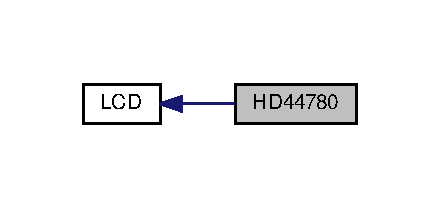
\includegraphics[width=238pt]{group___h_d44780}
\end{center}
\end{figure}
\subsection*{Strutture dati}
\begin{DoxyCompactItemize}
\item 
struct \hyperlink{struct_h_d44780___l_c_d__t}{H\+D44780\+\_\+\+L\+C\+D\+\_\+t}
\begin{DoxyCompactList}\small\item\em Struttura opaca che astrae un device Display L\+CD con cntroller Hitachi H\+D44780, o compatibile. Un oggetto di tipo \hyperlink{struct_h_d44780___l_c_d__t}{H\+D44780\+\_\+\+L\+C\+D\+\_\+t} rappresenta un device lcd H\+D44780. Il modulo è pensato per permettere la gestione di più display da parte dello stesso processore, agendo su oggetti \hyperlink{struct_h_d44780___l_c_d__t}{H\+D44780\+\_\+\+L\+C\+D\+\_\+t} diversi. Il modulo permette di utilizzare sia l\textquotesingle{}interfacciamento ad otto bit che quello a quattro bit, inizializzando il device opportunamente, attraverso l\textquotesingle{}uso delle funzioni H\+D44780\+\_\+\+Init8 e\+H\+D44780\+\_\+\+Init4. Il modulo fornisce anche semplici funzioni per la stampa di un carattere o di una stringa null-\/terminated di caratteri. Si veda la documentazione delle funzioni \hyperlink{group___h_d44780_ga57b8c6ca0b3c12e5f7273b3c373a6f17}{H\+D44780\+\_\+\+Printc()} e \hyperlink{group___h_d44780_ga3aedff8e2040e62db569fde955d3987b}{H\+D44780\+\_\+\+Print()}. Inoltre sono presenti diverse funzioni di utilità generica, come quelle per la pulizia del display, per lo spostamento del cursore di un posto in avanti o indietro, alla riga in basso o in alto. \end{DoxyCompactList}\end{DoxyCompactItemize}
\subsection*{Tipi enumerati (enum)}
\begin{DoxyCompactItemize}
\item 
enum \hyperlink{group___h_d44780_gaaaea8b73e24f7658da4118f6b01b45f0}{H\+D44780\+\_\+\+Interface\+Mode\+\_\+t} \{ \hyperlink{group___h_d44780_ggaaaea8b73e24f7658da4118f6b01b45f0a45bf6ce7ec7c951f692bdce9f0f485c6}{H\+D44780\+\_\+\+I\+N\+T\+E\+R\+F\+A\+C\+E\+\_\+4bit}, 
\hyperlink{group___h_d44780_ggaaaea8b73e24f7658da4118f6b01b45f0a24da9b234f9358c14184fe21f3c47de5}{H\+D44780\+\_\+\+I\+N\+T\+E\+R\+F\+A\+C\+E\+\_\+8bit}
 \}\begin{DoxyCompactList}\small\item\em Modalità di interfacciamento. Il modulo supporta sia interfacciamento a 4 bit che ad 8 bit. \end{DoxyCompactList}
\item 
enum \hyperlink{group___h_d44780_gaf46f4db4f981d3a1088804a6d6980d30}{H\+D44780\+\_\+\+Direction\+\_\+t} \{ \hyperlink{group___h_d44780_ggaf46f4db4f981d3a1088804a6d6980d30aa4d704398d4edd1e0dec8dbb55f90292}{H\+D44780\+\_\+\+Cursor\+Left}, 
\hyperlink{group___h_d44780_ggaf46f4db4f981d3a1088804a6d6980d30a26006ced693b6bab28c6e30bfdb8c399}{H\+D44780\+\_\+\+Cursor\+Right}
 \}\begin{DoxyCompactList}\small\item\em Direzioni di spostamento del cursore, usata dalla funzione \hyperlink{group___h_d44780_gabcea9a03050c46530e39b7556c673baf}{H\+D44780\+\_\+\+Move\+Cursor()} \end{DoxyCompactList}
\end{DoxyCompactItemize}
\subsection*{Funzioni}
\begin{DoxyCompactItemize}
\item 
void \hyperlink{group___h_d44780_gad212907e20316f4fc0e93d7c7a8f338e}{H\+D44780\+\_\+\+Init8} (\hyperlink{struct_h_d44780___l_c_d__t}{H\+D44780\+\_\+\+L\+C\+D\+\_\+t} $\ast$lcd, \hyperlink{structmy_g_p_i_o__t}{my\+G\+P\+I\+O\+\_\+t} $\ast$gpio, \hyperlink{group__bare-metal_ga402a0d20afc0cb7c25554b8b023f4253}{my\+G\+P\+I\+O\+\_\+mask} RS, \hyperlink{group__bare-metal_ga402a0d20afc0cb7c25554b8b023f4253}{my\+G\+P\+I\+O\+\_\+mask} RW, \hyperlink{group__bare-metal_ga402a0d20afc0cb7c25554b8b023f4253}{my\+G\+P\+I\+O\+\_\+mask} E, \hyperlink{group__bare-metal_ga402a0d20afc0cb7c25554b8b023f4253}{my\+G\+P\+I\+O\+\_\+mask} Data7, \hyperlink{group__bare-metal_ga402a0d20afc0cb7c25554b8b023f4253}{my\+G\+P\+I\+O\+\_\+mask} Data6, \hyperlink{group__bare-metal_ga402a0d20afc0cb7c25554b8b023f4253}{my\+G\+P\+I\+O\+\_\+mask} Data5, \hyperlink{group__bare-metal_ga402a0d20afc0cb7c25554b8b023f4253}{my\+G\+P\+I\+O\+\_\+mask} Data4, \hyperlink{group__bare-metal_ga402a0d20afc0cb7c25554b8b023f4253}{my\+G\+P\+I\+O\+\_\+mask} Data3, \hyperlink{group__bare-metal_ga402a0d20afc0cb7c25554b8b023f4253}{my\+G\+P\+I\+O\+\_\+mask} Data2, \hyperlink{group__bare-metal_ga402a0d20afc0cb7c25554b8b023f4253}{my\+G\+P\+I\+O\+\_\+mask} Data1, \hyperlink{group__bare-metal_ga402a0d20afc0cb7c25554b8b023f4253}{my\+G\+P\+I\+O\+\_\+mask} Data0)
\begin{DoxyCompactList}\small\item\em Inizializza un display lcd H\+D44780 con interfacciamento ad 8 bit. \end{DoxyCompactList}\item 
void \hyperlink{group___h_d44780_ga0c08f9e41d770ebfa4af385a56b47b81}{H\+D44780\+\_\+\+Init4} (\hyperlink{struct_h_d44780___l_c_d__t}{H\+D44780\+\_\+\+L\+C\+D\+\_\+t} $\ast$lcd, \hyperlink{structmy_g_p_i_o__t}{my\+G\+P\+I\+O\+\_\+t} $\ast$gpio, \hyperlink{group__bare-metal_ga402a0d20afc0cb7c25554b8b023f4253}{my\+G\+P\+I\+O\+\_\+mask} RS, \hyperlink{group__bare-metal_ga402a0d20afc0cb7c25554b8b023f4253}{my\+G\+P\+I\+O\+\_\+mask} RW, \hyperlink{group__bare-metal_ga402a0d20afc0cb7c25554b8b023f4253}{my\+G\+P\+I\+O\+\_\+mask} E, \hyperlink{group__bare-metal_ga402a0d20afc0cb7c25554b8b023f4253}{my\+G\+P\+I\+O\+\_\+mask} Data7, \hyperlink{group__bare-metal_ga402a0d20afc0cb7c25554b8b023f4253}{my\+G\+P\+I\+O\+\_\+mask} Data6, \hyperlink{group__bare-metal_ga402a0d20afc0cb7c25554b8b023f4253}{my\+G\+P\+I\+O\+\_\+mask} Data5, \hyperlink{group__bare-metal_ga402a0d20afc0cb7c25554b8b023f4253}{my\+G\+P\+I\+O\+\_\+mask} Data4)
\begin{DoxyCompactList}\small\item\em Inizializza un oggetto display lcd H\+D44780 affinché si utilizzi l\textquotesingle{}interfaccia a 4 bit. \end{DoxyCompactList}\item 
void \hyperlink{group___h_d44780_ga57b8c6ca0b3c12e5f7273b3c373a6f17}{H\+D44780\+\_\+\+Printc} (\hyperlink{struct_h_d44780___l_c_d__t}{H\+D44780\+\_\+\+L\+C\+D\+\_\+t} $\ast$lcd, char c)
\begin{DoxyCompactList}\small\item\em Stampa un carattere. \end{DoxyCompactList}\item 
void \hyperlink{group___h_d44780_ga3aedff8e2040e62db569fde955d3987b}{H\+D44780\+\_\+\+Print} (\hyperlink{struct_h_d44780___l_c_d__t}{H\+D44780\+\_\+\+L\+C\+D\+\_\+t} $\ast$lcd, const char $\ast$s)
\begin{DoxyCompactList}\small\item\em Stampa una stringa null-\/terminated di caratteri. \end{DoxyCompactList}\item 
void \hyperlink{group___h_d44780_ga2a5d4d528175321c46c790b581959e63}{H\+D44780\+\_\+print\+Binary8} (\hyperlink{struct_h_d44780___l_c_d__t}{H\+D44780\+\_\+\+L\+C\+D\+\_\+t} $\ast$lcd, uint8\+\_\+t b)
\begin{DoxyCompactList}\small\item\em Stampa un byte in binario. (bit più significativo a sinistra) \end{DoxyCompactList}\item 
void \hyperlink{group___h_d44780_ga95cceef2401c5519295e5a83c6688b5c}{H\+D44780\+\_\+print\+Binary32} (\hyperlink{struct_h_d44780___l_c_d__t}{H\+D44780\+\_\+\+L\+C\+D\+\_\+t} $\ast$lcd, uint32\+\_\+t w)
\begin{DoxyCompactList}\small\item\em Stampa una word di 32 bit in binario. (bit più significativo a sinistra) \end{DoxyCompactList}\item 
void \hyperlink{group___h_d44780_ga0f99bc5458acb172d0f3bfeb94f90e2a}{H\+D44780\+\_\+print\+Binary64} (\hyperlink{struct_h_d44780___l_c_d__t}{H\+D44780\+\_\+\+L\+C\+D\+\_\+t} $\ast$lcd, uint64\+\_\+t b)
\begin{DoxyCompactList}\small\item\em Stampa un blocco di 64 bit in binario. (bit più significativo a sinistra) \end{DoxyCompactList}\item 
void \hyperlink{group___h_d44780_gad967bd458b4d2bd358a93cbb7144addd}{H\+D44780\+\_\+print\+Hex8} (\hyperlink{struct_h_d44780___l_c_d__t}{H\+D44780\+\_\+\+L\+C\+D\+\_\+t} $\ast$lcd, uint8\+\_\+t b)
\begin{DoxyCompactList}\small\item\em Stampa un byte in esadecimale. (bit più significativo a sinistra) \end{DoxyCompactList}\item 
void \hyperlink{group___h_d44780_gaa82a2a27a3008f55c969a2d390c50497}{H\+D44780\+\_\+print\+Hex32} (\hyperlink{struct_h_d44780___l_c_d__t}{H\+D44780\+\_\+\+L\+C\+D\+\_\+t} $\ast$lcd, uint32\+\_\+t w)
\begin{DoxyCompactList}\small\item\em Stampa una word di 32 bit in esadecimale. (bit più significativo a sinistra) \end{DoxyCompactList}\item 
void \hyperlink{group___h_d44780_ga7a4b110e7da806f8c01e01d184d3a19a}{H\+D44780\+\_\+print\+Hex64} (\hyperlink{struct_h_d44780___l_c_d__t}{H\+D44780\+\_\+\+L\+C\+D\+\_\+t} $\ast$lcd, uint64\+\_\+t b)
\begin{DoxyCompactList}\small\item\em Stampa un blocco di 64 bit in esadecimale. (bit più significativo a sinistra) \end{DoxyCompactList}\item 
void \hyperlink{group___h_d44780_ga38cac13d7a66f068be54f79a716ff7d4}{H\+D44780\+\_\+\+Clear} (\hyperlink{struct_h_d44780___l_c_d__t}{H\+D44780\+\_\+\+L\+C\+D\+\_\+t} $\ast$lcd)
\begin{DoxyCompactList}\small\item\em Pulisce il display e sposta il cursore all\textquotesingle{}inizio della prima riga. \end{DoxyCompactList}\item 
void \hyperlink{group___h_d44780_ga68e3712332aa9482d4bdaa4991a92127}{H\+D44780\+\_\+\+Home} (\hyperlink{struct_h_d44780___l_c_d__t}{H\+D44780\+\_\+\+L\+C\+D\+\_\+t} $\ast$lcd)
\begin{DoxyCompactList}\small\item\em Sposta il cursore all\textquotesingle{}inizio della prima riga. \end{DoxyCompactList}\item 
void \hyperlink{group___h_d44780_gad90e2924a4e632ce42940323f8f49e37}{H\+D44780\+\_\+\+Move\+To\+Row1} (\hyperlink{struct_h_d44780___l_c_d__t}{H\+D44780\+\_\+\+L\+C\+D\+\_\+t} $\ast$lcd)
\begin{DoxyCompactList}\small\item\em Sposta il cursore all\textquotesingle{}inizio della prima riga. \end{DoxyCompactList}\item 
void \hyperlink{group___h_d44780_ga713670d498b6f5d50a174df19081c515}{H\+D44780\+\_\+\+Move\+To\+Row2} (\hyperlink{struct_h_d44780___l_c_d__t}{H\+D44780\+\_\+\+L\+C\+D\+\_\+t} $\ast$lcd)
\begin{DoxyCompactList}\small\item\em Sposta il cursore all\textquotesingle{}inizio della seconda riga. \end{DoxyCompactList}\item 
void \hyperlink{group___h_d44780_gabcea9a03050c46530e39b7556c673baf}{H\+D44780\+\_\+\+Move\+Cursor} (\hyperlink{struct_h_d44780___l_c_d__t}{H\+D44780\+\_\+\+L\+C\+D\+\_\+t} $\ast$lcd, \hyperlink{group___h_d44780_gaf46f4db4f981d3a1088804a6d6980d30}{H\+D44780\+\_\+\+Direction\+\_\+t} dir)
\begin{DoxyCompactList}\small\item\em Sposta il cursore di una posizione a destra o sinistra. \end{DoxyCompactList}\item 
void \hyperlink{group___h_d44780_ga5cf07b2179272029410f9a81f56621ed}{H\+D44780\+\_\+\+Display\+Off} (\hyperlink{struct_h_d44780___l_c_d__t}{H\+D44780\+\_\+\+L\+C\+D\+\_\+t} $\ast$lcd)
\begin{DoxyCompactList}\small\item\em Disattiva il display. \end{DoxyCompactList}\item 
void \hyperlink{group___h_d44780_ga56421dc398825188aa10257063a3ee4b}{H\+D44780\+\_\+\+Cursor\+Off} (\hyperlink{struct_h_d44780___l_c_d__t}{H\+D44780\+\_\+\+L\+C\+D\+\_\+t} $\ast$lcd)
\begin{DoxyCompactList}\small\item\em Disattiva la visualizzazione del cursore. \end{DoxyCompactList}\item 
void \hyperlink{group___h_d44780_ga3a381cb44df5d76d79be5ed71a52bae6}{H\+D44780\+\_\+\+Cursor\+On} (\hyperlink{struct_h_d44780___l_c_d__t}{H\+D44780\+\_\+\+L\+C\+D\+\_\+t} $\ast$lcd)
\begin{DoxyCompactList}\small\item\em Attiva la visualizzazione del cursore. \end{DoxyCompactList}\item 
void \hyperlink{group___h_d44780_ga92eb58cb7d73c9a87b7087a9c56f73d5}{H\+D44780\+\_\+\+Cursor\+Blink} (\hyperlink{struct_h_d44780___l_c_d__t}{H\+D44780\+\_\+\+L\+C\+D\+\_\+t} $\ast$lcd)
\begin{DoxyCompactList}\small\item\em Attiva il cursore lampeggiante. \end{DoxyCompactList}\end{DoxyCompactItemize}


\subsection{Descrizione dettagliata}
driver per display Hitachi hd44780 basato su driver my\+G\+P\+IO bare-\/metal 

Un oggetto di tipo \hyperlink{struct_h_d44780___l_c_d__t}{H\+D44780\+\_\+\+L\+C\+D\+\_\+t} rappresenta un device lcd H\+D44780. Il modulo è pensato per permettere la gestione di più display da parte dello stesso processore, agendo su oggetti \hyperlink{struct_h_d44780___l_c_d__t}{H\+D44780\+\_\+\+L\+C\+D\+\_\+t} diversi.~\newline
 La struttura \hyperlink{struct_h_d44780___l_c_d__t}{H\+D44780\+\_\+\+L\+C\+D\+\_\+t} specifica quali siano i pin del microcontrollore che pilotano un determinato segnale del device. L\textquotesingle{}assegnazione segnale-\/coppia, quindi l\textquotesingle{} inizializzazione della struttura \hyperlink{struct_h_d44780___l_c_d__t}{H\+D44780\+\_\+\+L\+C\+D\+\_\+t} relativa ad un device lcd, D\+E\+VE essere effettuata tassativamente utilizzando le funzioni~\newline

\begin{DoxyItemize}
\item \hyperlink{group___h_d44780_ga0c08f9e41d770ebfa4af385a56b47b81}{H\+D44780\+\_\+\+Init4()}
\item \hyperlink{group___h_d44780_gad212907e20316f4fc0e93d7c7a8f338e}{H\+D44780\+\_\+\+Init8()}~\newline

\end{DoxyItemize}

le quali provvedono anche ad effettuare un test di connessione volto ad individuare eventuali segnali erroneamente associati.~\newline


Oltre alle funzioni di inizializzazione, il modulo fornisce anche funzioni basilari per la stampa su display lcd di
\begin{DoxyItemize}
\item caratteri, con la funzione \hyperlink{group___h_d44780_ga57b8c6ca0b3c12e5f7273b3c373a6f17}{H\+D44780\+\_\+\+Printc()}
\item stringhe null-\/terminated di caratteri, con la funzione \hyperlink{group___h_d44780_ga3aedff8e2040e62db569fde955d3987b}{H\+D44780\+\_\+\+Print()}~\newline

\end{DoxyItemize}

Sono disponibili, inoltre, anche funzioni specifiche per inviare comandi al device\+:
\begin{DoxyItemize}
\item \hyperlink{group___h_d44780_ga38cac13d7a66f068be54f79a716ff7d4}{H\+D44780\+\_\+\+Clear()}
\item \hyperlink{group___h_d44780_ga68e3712332aa9482d4bdaa4991a92127}{H\+D44780\+\_\+\+Home()}
\item \hyperlink{group___h_d44780_gad90e2924a4e632ce42940323f8f49e37}{H\+D44780\+\_\+\+Move\+To\+Row1()}
\item \hyperlink{group___h_d44780_ga713670d498b6f5d50a174df19081c515}{H\+D44780\+\_\+\+Move\+To\+Row2()}
\item \hyperlink{group___h_d44780_gabcea9a03050c46530e39b7556c673baf}{H\+D44780\+\_\+\+Move\+Cursor()}
\item \hyperlink{group___h_d44780_ga5cf07b2179272029410f9a81f56621ed}{H\+D44780\+\_\+\+Display\+Off()}
\item \hyperlink{group___h_d44780_ga56421dc398825188aa10257063a3ee4b}{H\+D44780\+\_\+\+Cursor\+Off()}
\item \hyperlink{group___h_d44780_ga3a381cb44df5d76d79be5ed71a52bae6}{H\+D44780\+\_\+\+Cursor\+On()}
\item \hyperlink{group___h_d44780_ga92eb58cb7d73c9a87b7087a9c56f73d5}{H\+D44780\+\_\+\+Cursor\+Blink()}~\newline
 
\end{DoxyItemize}

\subsection{Documentazione dei tipi enumerati}
\mbox{\Hypertarget{group___h_d44780_gaf46f4db4f981d3a1088804a6d6980d30}\label{group___h_d44780_gaf46f4db4f981d3a1088804a6d6980d30}} 
\index{H\+D44780@{H\+D44780}!H\+D44780\+\_\+\+Direction\+\_\+t@{H\+D44780\+\_\+\+Direction\+\_\+t}}
\index{H\+D44780\+\_\+\+Direction\+\_\+t@{H\+D44780\+\_\+\+Direction\+\_\+t}!H\+D44780@{H\+D44780}}
\subsubsection{\texorpdfstring{H\+D44780\+\_\+\+Direction\+\_\+t}{HD44780\_Direction\_t}}
{\footnotesize\ttfamily enum \hyperlink{group___h_d44780_gaf46f4db4f981d3a1088804a6d6980d30}{H\+D44780\+\_\+\+Direction\+\_\+t}}



Direzioni di spostamento del cursore, usata dalla funzione \hyperlink{group___h_d44780_gabcea9a03050c46530e39b7556c673baf}{H\+D44780\+\_\+\+Move\+Cursor()} 

\begin{DoxyEnumFields}{Valori del tipo enumerato}
\raisebox{\heightof{T}}[0pt][0pt]{\index{H\+D44780\+\_\+\+Cursor\+Left@{H\+D44780\+\_\+\+Cursor\+Left}!H\+D44780@{H\+D44780}}\index{H\+D44780@{H\+D44780}!H\+D44780\+\_\+\+Cursor\+Left@{H\+D44780\+\_\+\+Cursor\+Left}}}\mbox{\Hypertarget{group___h_d44780_ggaf46f4db4f981d3a1088804a6d6980d30aa4d704398d4edd1e0dec8dbb55f90292}\label{group___h_d44780_ggaf46f4db4f981d3a1088804a6d6980d30aa4d704398d4edd1e0dec8dbb55f90292}} 
H\+D44780\+\_\+\+Cursor\+Left&left sposta il cursore a sinistra \\
\hline

\raisebox{\heightof{T}}[0pt][0pt]{\index{H\+D44780\+\_\+\+Cursor\+Right@{H\+D44780\+\_\+\+Cursor\+Right}!H\+D44780@{H\+D44780}}\index{H\+D44780@{H\+D44780}!H\+D44780\+\_\+\+Cursor\+Right@{H\+D44780\+\_\+\+Cursor\+Right}}}\mbox{\Hypertarget{group___h_d44780_ggaf46f4db4f981d3a1088804a6d6980d30a26006ced693b6bab28c6e30bfdb8c399}\label{group___h_d44780_ggaf46f4db4f981d3a1088804a6d6980d30a26006ced693b6bab28c6e30bfdb8c399}} 
H\+D44780\+\_\+\+Cursor\+Right&right sposta il cursore a destra \\
\hline

\end{DoxyEnumFields}
\mbox{\Hypertarget{group___h_d44780_gaaaea8b73e24f7658da4118f6b01b45f0}\label{group___h_d44780_gaaaea8b73e24f7658da4118f6b01b45f0}} 
\index{H\+D44780@{H\+D44780}!H\+D44780\+\_\+\+Interface\+Mode\+\_\+t@{H\+D44780\+\_\+\+Interface\+Mode\+\_\+t}}
\index{H\+D44780\+\_\+\+Interface\+Mode\+\_\+t@{H\+D44780\+\_\+\+Interface\+Mode\+\_\+t}!H\+D44780@{H\+D44780}}
\subsubsection{\texorpdfstring{H\+D44780\+\_\+\+Interface\+Mode\+\_\+t}{HD44780\_InterfaceMode\_t}}
{\footnotesize\ttfamily enum \hyperlink{group___h_d44780_gaaaea8b73e24f7658da4118f6b01b45f0}{H\+D44780\+\_\+\+Interface\+Mode\+\_\+t}}



Modalità di interfacciamento. Il modulo supporta sia interfacciamento a 4 bit che ad 8 bit. 

\begin{DoxyEnumFields}{Valori del tipo enumerato}
\raisebox{\heightof{T}}[0pt][0pt]{\index{H\+D44780\+\_\+\+I\+N\+T\+E\+R\+F\+A\+C\+E\+\_\+4bit@{H\+D44780\+\_\+\+I\+N\+T\+E\+R\+F\+A\+C\+E\+\_\+4bit}!H\+D44780@{H\+D44780}}\index{H\+D44780@{H\+D44780}!H\+D44780\+\_\+\+I\+N\+T\+E\+R\+F\+A\+C\+E\+\_\+4bit@{H\+D44780\+\_\+\+I\+N\+T\+E\+R\+F\+A\+C\+E\+\_\+4bit}}}\mbox{\Hypertarget{group___h_d44780_ggaaaea8b73e24f7658da4118f6b01b45f0a45bf6ce7ec7c951f692bdce9f0f485c6}\label{group___h_d44780_ggaaaea8b73e24f7658da4118f6b01b45f0a45bf6ce7ec7c951f692bdce9f0f485c6}} 
H\+D44780\+\_\+\+I\+N\+T\+E\+R\+F\+A\+C\+E\+\_\+4bit&Interfacciamento a quattro bit \\
\hline

\raisebox{\heightof{T}}[0pt][0pt]{\index{H\+D44780\+\_\+\+I\+N\+T\+E\+R\+F\+A\+C\+E\+\_\+8bit@{H\+D44780\+\_\+\+I\+N\+T\+E\+R\+F\+A\+C\+E\+\_\+8bit}!H\+D44780@{H\+D44780}}\index{H\+D44780@{H\+D44780}!H\+D44780\+\_\+\+I\+N\+T\+E\+R\+F\+A\+C\+E\+\_\+8bit@{H\+D44780\+\_\+\+I\+N\+T\+E\+R\+F\+A\+C\+E\+\_\+8bit}}}\mbox{\Hypertarget{group___h_d44780_ggaaaea8b73e24f7658da4118f6b01b45f0a24da9b234f9358c14184fe21f3c47de5}\label{group___h_d44780_ggaaaea8b73e24f7658da4118f6b01b45f0a24da9b234f9358c14184fe21f3c47de5}} 
H\+D44780\+\_\+\+I\+N\+T\+E\+R\+F\+A\+C\+E\+\_\+8bit&Interfacciamento ad otto bit \\
\hline

\end{DoxyEnumFields}


\subsection{Documentazione delle funzioni}
\mbox{\Hypertarget{group___h_d44780_ga38cac13d7a66f068be54f79a716ff7d4}\label{group___h_d44780_ga38cac13d7a66f068be54f79a716ff7d4}} 
\index{H\+D44780@{H\+D44780}!H\+D44780\+\_\+\+Clear@{H\+D44780\+\_\+\+Clear}}
\index{H\+D44780\+\_\+\+Clear@{H\+D44780\+\_\+\+Clear}!H\+D44780@{H\+D44780}}
\subsubsection{\texorpdfstring{H\+D44780\+\_\+\+Clear()}{HD44780\_Clear()}}
{\footnotesize\ttfamily void H\+D44780\+\_\+\+Clear (\begin{DoxyParamCaption}\item[{\hyperlink{struct_h_d44780___l_c_d__t}{H\+D44780\+\_\+\+L\+C\+D\+\_\+t} $\ast$}]{lcd }\end{DoxyParamCaption})}



Pulisce il display e sposta il cursore all\textquotesingle{}inizio della prima riga. 


\begin{DoxyParams}[1]{Parametri}
\mbox{\tt in}  & {\em lcd} & display da pilotare; \\
\hline
\end{DoxyParams}
\mbox{\Hypertarget{group___h_d44780_ga92eb58cb7d73c9a87b7087a9c56f73d5}\label{group___h_d44780_ga92eb58cb7d73c9a87b7087a9c56f73d5}} 
\index{H\+D44780@{H\+D44780}!H\+D44780\+\_\+\+Cursor\+Blink@{H\+D44780\+\_\+\+Cursor\+Blink}}
\index{H\+D44780\+\_\+\+Cursor\+Blink@{H\+D44780\+\_\+\+Cursor\+Blink}!H\+D44780@{H\+D44780}}
\subsubsection{\texorpdfstring{H\+D44780\+\_\+\+Cursor\+Blink()}{HD44780\_CursorBlink()}}
{\footnotesize\ttfamily void H\+D44780\+\_\+\+Cursor\+Blink (\begin{DoxyParamCaption}\item[{\hyperlink{struct_h_d44780___l_c_d__t}{H\+D44780\+\_\+\+L\+C\+D\+\_\+t} $\ast$}]{lcd }\end{DoxyParamCaption})}



Attiva il cursore lampeggiante. 


\begin{DoxyParams}[1]{Parametri}
\mbox{\tt in}  & {\em lcd} & display da pilotare; \\
\hline
\end{DoxyParams}
\mbox{\Hypertarget{group___h_d44780_ga56421dc398825188aa10257063a3ee4b}\label{group___h_d44780_ga56421dc398825188aa10257063a3ee4b}} 
\index{H\+D44780@{H\+D44780}!H\+D44780\+\_\+\+Cursor\+Off@{H\+D44780\+\_\+\+Cursor\+Off}}
\index{H\+D44780\+\_\+\+Cursor\+Off@{H\+D44780\+\_\+\+Cursor\+Off}!H\+D44780@{H\+D44780}}
\subsubsection{\texorpdfstring{H\+D44780\+\_\+\+Cursor\+Off()}{HD44780\_CursorOff()}}
{\footnotesize\ttfamily void H\+D44780\+\_\+\+Cursor\+Off (\begin{DoxyParamCaption}\item[{\hyperlink{struct_h_d44780___l_c_d__t}{H\+D44780\+\_\+\+L\+C\+D\+\_\+t} $\ast$}]{lcd }\end{DoxyParamCaption})}



Disattiva la visualizzazione del cursore. 


\begin{DoxyParams}[1]{Parametri}
\mbox{\tt in}  & {\em lcd} & display da pilotare; \\
\hline
\end{DoxyParams}
\mbox{\Hypertarget{group___h_d44780_ga3a381cb44df5d76d79be5ed71a52bae6}\label{group___h_d44780_ga3a381cb44df5d76d79be5ed71a52bae6}} 
\index{H\+D44780@{H\+D44780}!H\+D44780\+\_\+\+Cursor\+On@{H\+D44780\+\_\+\+Cursor\+On}}
\index{H\+D44780\+\_\+\+Cursor\+On@{H\+D44780\+\_\+\+Cursor\+On}!H\+D44780@{H\+D44780}}
\subsubsection{\texorpdfstring{H\+D44780\+\_\+\+Cursor\+On()}{HD44780\_CursorOn()}}
{\footnotesize\ttfamily void H\+D44780\+\_\+\+Cursor\+On (\begin{DoxyParamCaption}\item[{\hyperlink{struct_h_d44780___l_c_d__t}{H\+D44780\+\_\+\+L\+C\+D\+\_\+t} $\ast$}]{lcd }\end{DoxyParamCaption})}



Attiva la visualizzazione del cursore. 


\begin{DoxyParams}[1]{Parametri}
\mbox{\tt in}  & {\em lcd} & display da pilotare; \\
\hline
\end{DoxyParams}
\mbox{\Hypertarget{group___h_d44780_ga5cf07b2179272029410f9a81f56621ed}\label{group___h_d44780_ga5cf07b2179272029410f9a81f56621ed}} 
\index{H\+D44780@{H\+D44780}!H\+D44780\+\_\+\+Display\+Off@{H\+D44780\+\_\+\+Display\+Off}}
\index{H\+D44780\+\_\+\+Display\+Off@{H\+D44780\+\_\+\+Display\+Off}!H\+D44780@{H\+D44780}}
\subsubsection{\texorpdfstring{H\+D44780\+\_\+\+Display\+Off()}{HD44780\_DisplayOff()}}
{\footnotesize\ttfamily void H\+D44780\+\_\+\+Display\+Off (\begin{DoxyParamCaption}\item[{\hyperlink{struct_h_d44780___l_c_d__t}{H\+D44780\+\_\+\+L\+C\+D\+\_\+t} $\ast$}]{lcd }\end{DoxyParamCaption})}



Disattiva il display. 


\begin{DoxyParams}[1]{Parametri}
\mbox{\tt in}  & {\em lcd} & display da pilotare; \\
\hline
\end{DoxyParams}
\mbox{\Hypertarget{group___h_d44780_ga68e3712332aa9482d4bdaa4991a92127}\label{group___h_d44780_ga68e3712332aa9482d4bdaa4991a92127}} 
\index{H\+D44780@{H\+D44780}!H\+D44780\+\_\+\+Home@{H\+D44780\+\_\+\+Home}}
\index{H\+D44780\+\_\+\+Home@{H\+D44780\+\_\+\+Home}!H\+D44780@{H\+D44780}}
\subsubsection{\texorpdfstring{H\+D44780\+\_\+\+Home()}{HD44780\_Home()}}
{\footnotesize\ttfamily void H\+D44780\+\_\+\+Home (\begin{DoxyParamCaption}\item[{\hyperlink{struct_h_d44780___l_c_d__t}{H\+D44780\+\_\+\+L\+C\+D\+\_\+t} $\ast$}]{lcd }\end{DoxyParamCaption})}



Sposta il cursore all\textquotesingle{}inizio della prima riga. 


\begin{DoxyParams}[1]{Parametri}
\mbox{\tt in}  & {\em lcd} & display da pilotare; \\
\hline
\end{DoxyParams}
\mbox{\Hypertarget{group___h_d44780_ga0c08f9e41d770ebfa4af385a56b47b81}\label{group___h_d44780_ga0c08f9e41d770ebfa4af385a56b47b81}} 
\index{H\+D44780@{H\+D44780}!H\+D44780\+\_\+\+Init4@{H\+D44780\+\_\+\+Init4}}
\index{H\+D44780\+\_\+\+Init4@{H\+D44780\+\_\+\+Init4}!H\+D44780@{H\+D44780}}
\subsubsection{\texorpdfstring{H\+D44780\+\_\+\+Init4()}{HD44780\_Init4()}}
{\footnotesize\ttfamily void H\+D44780\+\_\+\+Init4 (\begin{DoxyParamCaption}\item[{\hyperlink{struct_h_d44780___l_c_d__t}{H\+D44780\+\_\+\+L\+C\+D\+\_\+t} $\ast$}]{lcd,  }\item[{\hyperlink{structmy_g_p_i_o__t}{my\+G\+P\+I\+O\+\_\+t} $\ast$}]{gpio,  }\item[{\hyperlink{group__bare-metal_ga402a0d20afc0cb7c25554b8b023f4253}{my\+G\+P\+I\+O\+\_\+mask}}]{RS,  }\item[{\hyperlink{group__bare-metal_ga402a0d20afc0cb7c25554b8b023f4253}{my\+G\+P\+I\+O\+\_\+mask}}]{RW,  }\item[{\hyperlink{group__bare-metal_ga402a0d20afc0cb7c25554b8b023f4253}{my\+G\+P\+I\+O\+\_\+mask}}]{E,  }\item[{\hyperlink{group__bare-metal_ga402a0d20afc0cb7c25554b8b023f4253}{my\+G\+P\+I\+O\+\_\+mask}}]{Data7,  }\item[{\hyperlink{group__bare-metal_ga402a0d20afc0cb7c25554b8b023f4253}{my\+G\+P\+I\+O\+\_\+mask}}]{Data6,  }\item[{\hyperlink{group__bare-metal_ga402a0d20afc0cb7c25554b8b023f4253}{my\+G\+P\+I\+O\+\_\+mask}}]{Data5,  }\item[{\hyperlink{group__bare-metal_ga402a0d20afc0cb7c25554b8b023f4253}{my\+G\+P\+I\+O\+\_\+mask}}]{Data4 }\end{DoxyParamCaption})}



Inizializza un oggetto display lcd H\+D44780 affinché si utilizzi l\textquotesingle{}interfaccia a 4 bit. 

Inizializza un oggetto \hyperlink{struct_h_d44780___l_c_d__t}{H\+D44780\+\_\+\+L\+C\+D\+\_\+t} verificando la validità delle coppie porta-\/pin per l\textquotesingle{} interfacciamento, configurando i pin my\+G\+P\+IO e inizializzando il device.

\begin{DoxyWarning}{Avvertimento}
Se i pin associati ai segnali di pilotaggio del device non sono correttamente configurati come pin di output, il dispositivo non funzionerà correttamente.

Non modificare i campi della struttura \hyperlink{struct_h_d44780___l_c_d__t}{H\+D44780\+\_\+\+L\+C\+D\+\_\+t} dopo che essa sia stata inizializzata.

La struttura \hyperlink{structmy_g_p_i_o__t}{my\+G\+P\+I\+O\+\_\+t}, a cui fa riferimento il parametro gpio, va inizializzata a parte.
\end{DoxyWarning}

\begin{DoxyParams}[1]{Parametri}
\mbox{\tt in,out}  & {\em lcd} & puntatore a struttura di tipo \hyperlink{struct_h_d44780___l_c_d__t}{H\+D44780\+\_\+\+L\+C\+D\+\_\+t} che descrive un display H\+D44780 da inizializzare; \\
\hline
\mbox{\tt in}  & {\em gpio} & puntatore alla struttura \hyperlink{structmy_g_p_i_o__t}{my\+G\+P\+I\+O\+\_\+t} che astrae il device my\+G\+P\+IO a cui il display è connesso. Non viene inizializzato dalla funziona, sarà necessario inizializzarlo preventivamente; \\
\hline
\mbox{\tt in}  & {\em RS} & pin del device my\+G\+P\+IO a cui è associato il segnale RS (data/command) del display L\+CD; \\
\hline
\mbox{\tt in}  & {\em RW} & pin del device my\+G\+P\+IO a cui è associato il segnale RW (read/write) del display L\+CD; \\
\hline
\mbox{\tt in}  & {\em E} & pin del device my\+G\+P\+IO a cui è associato il segnale E (Enable) del display L\+CD; \\
\hline
\mbox{\tt in}  & {\em Data7} & pin del device my\+G\+P\+IO a cui è associato il segnale Data7 del display L\+CD; \\
\hline
\mbox{\tt in}  & {\em Data6} & pin del device my\+G\+P\+IO a cui è associato il segnale Data6 del display L\+CD; \\
\hline
\mbox{\tt in}  & {\em Data5} & pin del device my\+G\+P\+IO a cui è associato il segnale Data5 del display L\+CD; \\
\hline
\mbox{\tt in}  & {\em Data4} & pin del device my\+G\+P\+IO a cui è associato il segnale Data4 del display L\+CD;\\
\hline
\end{DoxyParams}

\begin{DoxyCode}
\hyperlink{structmy_g_p_i_o__t}{myGPIO\_t} gpioDisplay;
GPIO\_init(&gpioDisplay, XPAR\_MYGPIO\_3\_S00\_AXI\_BASEADDR, 11, 0, 4, 8);
\hyperlink{struct_h_d44780___l_c_d__t}{HD44780\_LCD\_t} lcd;
\hyperlink{group___h_d44780_ga0c08f9e41d770ebfa4af385a56b47b81}{HD44780\_Init4}(&lcd, &gpioDisplay,   GPIO\_pin10, GPIO\_pin9, GPIO\_pin8,
                                        GPIO\_pin0, GPIO\_pin1, GPIO\_pin2, GPIO\_pin3);
\hyperlink{group___h_d44780_ga3aedff8e2040e62db569fde955d3987b}{HD44780\_Print}(&lcd, \textcolor{stringliteral}{"Ciao! Come va"});
\hyperlink{group___h_d44780_ga713670d498b6f5d50a174df19081c515}{HD44780\_MoveToRow2}(&lcd);
\hyperlink{group___h_d44780_ga3aedff8e2040e62db569fde955d3987b}{HD44780\_Print}(&lcd, \textcolor{stringliteral}{"lo studio?"});
\end{DoxyCode}
 \mbox{\Hypertarget{group___h_d44780_gad212907e20316f4fc0e93d7c7a8f338e}\label{group___h_d44780_gad212907e20316f4fc0e93d7c7a8f338e}} 
\index{H\+D44780@{H\+D44780}!H\+D44780\+\_\+\+Init8@{H\+D44780\+\_\+\+Init8}}
\index{H\+D44780\+\_\+\+Init8@{H\+D44780\+\_\+\+Init8}!H\+D44780@{H\+D44780}}
\subsubsection{\texorpdfstring{H\+D44780\+\_\+\+Init8()}{HD44780\_Init8()}}
{\footnotesize\ttfamily void H\+D44780\+\_\+\+Init8 (\begin{DoxyParamCaption}\item[{\hyperlink{struct_h_d44780___l_c_d__t}{H\+D44780\+\_\+\+L\+C\+D\+\_\+t} $\ast$}]{lcd,  }\item[{\hyperlink{structmy_g_p_i_o__t}{my\+G\+P\+I\+O\+\_\+t} $\ast$}]{gpio,  }\item[{\hyperlink{group__bare-metal_ga402a0d20afc0cb7c25554b8b023f4253}{my\+G\+P\+I\+O\+\_\+mask}}]{RS,  }\item[{\hyperlink{group__bare-metal_ga402a0d20afc0cb7c25554b8b023f4253}{my\+G\+P\+I\+O\+\_\+mask}}]{RW,  }\item[{\hyperlink{group__bare-metal_ga402a0d20afc0cb7c25554b8b023f4253}{my\+G\+P\+I\+O\+\_\+mask}}]{E,  }\item[{\hyperlink{group__bare-metal_ga402a0d20afc0cb7c25554b8b023f4253}{my\+G\+P\+I\+O\+\_\+mask}}]{Data7,  }\item[{\hyperlink{group__bare-metal_ga402a0d20afc0cb7c25554b8b023f4253}{my\+G\+P\+I\+O\+\_\+mask}}]{Data6,  }\item[{\hyperlink{group__bare-metal_ga402a0d20afc0cb7c25554b8b023f4253}{my\+G\+P\+I\+O\+\_\+mask}}]{Data5,  }\item[{\hyperlink{group__bare-metal_ga402a0d20afc0cb7c25554b8b023f4253}{my\+G\+P\+I\+O\+\_\+mask}}]{Data4,  }\item[{\hyperlink{group__bare-metal_ga402a0d20afc0cb7c25554b8b023f4253}{my\+G\+P\+I\+O\+\_\+mask}}]{Data3,  }\item[{\hyperlink{group__bare-metal_ga402a0d20afc0cb7c25554b8b023f4253}{my\+G\+P\+I\+O\+\_\+mask}}]{Data2,  }\item[{\hyperlink{group__bare-metal_ga402a0d20afc0cb7c25554b8b023f4253}{my\+G\+P\+I\+O\+\_\+mask}}]{Data1,  }\item[{\hyperlink{group__bare-metal_ga402a0d20afc0cb7c25554b8b023f4253}{my\+G\+P\+I\+O\+\_\+mask}}]{Data0 }\end{DoxyParamCaption})}



Inizializza un display lcd H\+D44780 con interfacciamento ad 8 bit. 

\begin{DoxyWarning}{Avvertimento}
Se i pin associati ai segnali di pilotaggio del device non sono correttamente configurati come pin di output, il dispositivo non funzionerà correttamente.

Non modificare i campi della struttura dopo che essa sia stata inizializzata.

La struttura \hyperlink{structmy_g_p_i_o__t}{my\+G\+P\+I\+O\+\_\+t}, a cui fa riferimento il parametro gpio, va inizializzata a parte.
\end{DoxyWarning}

\begin{DoxyParams}[1]{Parametri}
\mbox{\tt in,out}  & {\em lcd} & puntatore a struttura di tipo \hyperlink{struct_h_d44780___l_c_d__t}{H\+D44780\+\_\+\+L\+C\+D\+\_\+t} che descrive un display H\+D44780 da inizializzare; \\
\hline
\mbox{\tt in}  & {\em gpio} & puntatore alla struttura \hyperlink{structmy_g_p_i_o__t}{my\+G\+P\+I\+O\+\_\+t} che astrae il device my\+G\+P\+IO a cui il display è connesso. Non viene inizializzato dalla funziona, sarà necessario inizializzarlo preventivamente; \\
\hline
\mbox{\tt in}  & {\em RS} & pin del device my\+G\+P\+IO a cui è associato il segnale RS (data/command) del display L\+CD; \\
\hline
\mbox{\tt in}  & {\em RW} & pin del device my\+G\+P\+IO a cui è associato il segnale RW (read/write) del display L\+CD; \\
\hline
\mbox{\tt in}  & {\em E} & pin del device my\+G\+P\+IO a cui è associato il segnale E (Enable) del display L\+CD; \\
\hline
\mbox{\tt in}  & {\em Data7} & pin del device my\+G\+P\+IO a cui è associato il segnale Data7 del display L\+CD; \\
\hline
\mbox{\tt in}  & {\em Data6} & pin del device my\+G\+P\+IO a cui è associato il segnale Data6 del display L\+CD; \\
\hline
\mbox{\tt in}  & {\em Data5} & pin del device my\+G\+P\+IO a cui è associato il segnale Data5 del display L\+CD; \\
\hline
\mbox{\tt in}  & {\em Data4} & pin del device my\+G\+P\+IO a cui è associato il segnale Data4 del display L\+CD; \\
\hline
\mbox{\tt in}  & {\em Data3} & pin del device my\+G\+P\+IO a cui è associato il segnale Data3 del display L\+CD; \\
\hline
\mbox{\tt in}  & {\em Data2} & pin del device my\+G\+P\+IO a cui è associato il segnale Data2 del display L\+CD; \\
\hline
\mbox{\tt in}  & {\em Data1} & pin del device my\+G\+P\+IO a cui è associato il segnale Data1 del display L\+CD; \\
\hline
\mbox{\tt in}  & {\em Data0} & pin del device my\+G\+P\+IO a cui è associato il segnale Data0 del display L\+CD;\\
\hline
\end{DoxyParams}

\begin{DoxyCode}
\hyperlink{structmy_g_p_i_o__t}{myGPIO\_t} gpioDisplay;
\hyperlink{group__bare-metal_ga588201358d1633c53535b288c9198531}{myGPIO\_Init}(&gpioDisplay, XPAR\_MYGPIO\_3\_S00\_AXI\_BASEADDR);
\hyperlink{struct_h_d44780___l_c_d__t}{HD44780\_LCD\_t} lcd;
\hyperlink{group___h_d44780_gad212907e20316f4fc0e93d7c7a8f338e}{HD44780\_Init8}(&lcd, &gpioDisplay,   GPIO\_pin10, GPIO\_pin9, GPIO\_pin8,
                                        GPIO\_pin0, GPIO\_pin1, GPIO\_pin2, GPIO\_pin3,
                                    GPIO\_pin4, GPIO\_pin5, GPIO\_pin6, GPIO\_pin7);
\hyperlink{group___h_d44780_ga3aedff8e2040e62db569fde955d3987b}{HD44780\_Print}(&lcd, \textcolor{stringliteral}{"Ciao! Come va"});
\hyperlink{group___h_d44780_ga713670d498b6f5d50a174df19081c515}{HD44780\_MoveToRow2}(&lcd);
\hyperlink{group___h_d44780_ga3aedff8e2040e62db569fde955d3987b}{HD44780\_Print}(&lcd, \textcolor{stringliteral}{"lo studio?"});
\end{DoxyCode}
 \mbox{\Hypertarget{group___h_d44780_gabcea9a03050c46530e39b7556c673baf}\label{group___h_d44780_gabcea9a03050c46530e39b7556c673baf}} 
\index{H\+D44780@{H\+D44780}!H\+D44780\+\_\+\+Move\+Cursor@{H\+D44780\+\_\+\+Move\+Cursor}}
\index{H\+D44780\+\_\+\+Move\+Cursor@{H\+D44780\+\_\+\+Move\+Cursor}!H\+D44780@{H\+D44780}}
\subsubsection{\texorpdfstring{H\+D44780\+\_\+\+Move\+Cursor()}{HD44780\_MoveCursor()}}
{\footnotesize\ttfamily void H\+D44780\+\_\+\+Move\+Cursor (\begin{DoxyParamCaption}\item[{\hyperlink{struct_h_d44780___l_c_d__t}{H\+D44780\+\_\+\+L\+C\+D\+\_\+t} $\ast$}]{lcd,  }\item[{\hyperlink{group___h_d44780_gaf46f4db4f981d3a1088804a6d6980d30}{H\+D44780\+\_\+\+Direction\+\_\+t}}]{dir }\end{DoxyParamCaption})}



Sposta il cursore di una posizione a destra o sinistra. 


\begin{DoxyParams}[1]{Parametri}
\mbox{\tt in}  & {\em lcd} & display da pilotare; \\
\hline
\mbox{\tt in}  & {\em dir} & direzione in cui spostare il cursore, \\
\hline
\end{DoxyParams}
\begin{DoxySeeAlso}{Si veda anche}
direction\+\_\+t; 
\end{DoxySeeAlso}
\mbox{\Hypertarget{group___h_d44780_gad90e2924a4e632ce42940323f8f49e37}\label{group___h_d44780_gad90e2924a4e632ce42940323f8f49e37}} 
\index{H\+D44780@{H\+D44780}!H\+D44780\+\_\+\+Move\+To\+Row1@{H\+D44780\+\_\+\+Move\+To\+Row1}}
\index{H\+D44780\+\_\+\+Move\+To\+Row1@{H\+D44780\+\_\+\+Move\+To\+Row1}!H\+D44780@{H\+D44780}}
\subsubsection{\texorpdfstring{H\+D44780\+\_\+\+Move\+To\+Row1()}{HD44780\_MoveToRow1()}}
{\footnotesize\ttfamily void H\+D44780\+\_\+\+Move\+To\+Row1 (\begin{DoxyParamCaption}\item[{\hyperlink{struct_h_d44780___l_c_d__t}{H\+D44780\+\_\+\+L\+C\+D\+\_\+t} $\ast$}]{lcd }\end{DoxyParamCaption})}



Sposta il cursore all\textquotesingle{}inizio della prima riga. 


\begin{DoxyParams}[1]{Parametri}
\mbox{\tt in}  & {\em lcd} & display da pilotare; \\
\hline
\end{DoxyParams}
\mbox{\Hypertarget{group___h_d44780_ga713670d498b6f5d50a174df19081c515}\label{group___h_d44780_ga713670d498b6f5d50a174df19081c515}} 
\index{H\+D44780@{H\+D44780}!H\+D44780\+\_\+\+Move\+To\+Row2@{H\+D44780\+\_\+\+Move\+To\+Row2}}
\index{H\+D44780\+\_\+\+Move\+To\+Row2@{H\+D44780\+\_\+\+Move\+To\+Row2}!H\+D44780@{H\+D44780}}
\subsubsection{\texorpdfstring{H\+D44780\+\_\+\+Move\+To\+Row2()}{HD44780\_MoveToRow2()}}
{\footnotesize\ttfamily void H\+D44780\+\_\+\+Move\+To\+Row2 (\begin{DoxyParamCaption}\item[{\hyperlink{struct_h_d44780___l_c_d__t}{H\+D44780\+\_\+\+L\+C\+D\+\_\+t} $\ast$}]{lcd }\end{DoxyParamCaption})}



Sposta il cursore all\textquotesingle{}inizio della seconda riga. 


\begin{DoxyParams}[1]{Parametri}
\mbox{\tt in}  & {\em lcd} & display da pilotare; \\
\hline
\end{DoxyParams}
\mbox{\Hypertarget{group___h_d44780_ga3aedff8e2040e62db569fde955d3987b}\label{group___h_d44780_ga3aedff8e2040e62db569fde955d3987b}} 
\index{H\+D44780@{H\+D44780}!H\+D44780\+\_\+\+Print@{H\+D44780\+\_\+\+Print}}
\index{H\+D44780\+\_\+\+Print@{H\+D44780\+\_\+\+Print}!H\+D44780@{H\+D44780}}
\subsubsection{\texorpdfstring{H\+D44780\+\_\+\+Print()}{HD44780\_Print()}}
{\footnotesize\ttfamily void H\+D44780\+\_\+\+Print (\begin{DoxyParamCaption}\item[{\hyperlink{struct_h_d44780___l_c_d__t}{H\+D44780\+\_\+\+L\+C\+D\+\_\+t} $\ast$}]{lcd,  }\item[{const char $\ast$}]{s }\end{DoxyParamCaption})}



Stampa una stringa null-\/terminated di caratteri. 

La funzione può essere utilizzata per stampare anche numeri interi e floating point. Si veda gli esempi di cui sotto.


\begin{DoxyParams}[1]{Parametri}
\mbox{\tt in}  & {\em lcd} & display da pilotare; \\
\hline
\mbox{\tt in}  & {\em s} & puntatore alla stringa null-\/terminated da stampare sul display;\\
\hline
\end{DoxyParams}

\begin{DoxyCode}
\textcolor{comment}{// stampa di un intero}
\textcolor{preprocessor}{#include <stdlib.h>}
    ...
char str[10];   \textcolor{comment}{// assicurarsi di allocare sufficiente spazio per la stampa del numero}
sprintf(str,\textcolor{stringliteral}{"%d"}, integer\_number);
error = \hyperlink{group___h_d44780_ga3aedff8e2040e62db569fde955d3987b}{HD44780\_Print}(lcd, str);
\end{DoxyCode}



\begin{DoxyCode}
\textcolor{comment}{// stampa di un intero}
\textcolor{preprocessor}{#include <stdlib.h>}
...
char str[10];
snprintf(str, 10,\textcolor{stringliteral}{"%d"}, integer\_number);
error = \hyperlink{group___h_d44780_ga3aedff8e2040e62db569fde955d3987b}{HD44780\_Print}(lcd, str);
\end{DoxyCode}



\begin{DoxyCode}
\textcolor{comment}{// stampa di un float}
\textcolor{preprocessor}{#include <stdlib.h>}
...
char str[20];   \textcolor{comment}{// assicurarsi di allocare sufficiente spazio per la stampa del numero}
sprintf(str,\textcolor{stringliteral}{"%f"}, float\_number);
error = \hyperlink{group___h_d44780_ga3aedff8e2040e62db569fde955d3987b}{HD44780\_Print}(lcd, str);
\end{DoxyCode}



\begin{DoxyCode}
\textcolor{comment}{// stampa di un float, nel caso in cui la soluzione precedente dovesse non funzionare}
\textcolor{preprocessor}{#include <stdlib.h>}
...
char str[20];
\textcolor{keywordtype}{int} parte\_intera, parte\_decimale, moltiplicatore = 1000;
\textcolor{comment}{// se si desiderano più di tre cifre decimali basta aumentare la potenza del}
\textcolor{comment}{// moltiplicatore}
\textcolor{comment}{// es. cinque cifre decimali ==> moltiplicatore = 100000}
\textcolor{comment}{// si sconsiglia di stampare più di quattro cifre decimali per non causare overflow}
\textcolor{comment}{// nelle istruzioni che seguono}
parte\_intera = (int) float\_number;
parte\_decimale = (int)(float\_number * moltiplicatore) - (parte\_intera * moltiplicatore);
snprintf(str, 20,\textcolor{stringliteral}{"%d.%d"}, parte\_intera, parte\_decimale);
error = \hyperlink{group___h_d44780_ga3aedff8e2040e62db569fde955d3987b}{HD44780\_Print}(lcd, str);
\end{DoxyCode}
 \mbox{\Hypertarget{group___h_d44780_ga95cceef2401c5519295e5a83c6688b5c}\label{group___h_d44780_ga95cceef2401c5519295e5a83c6688b5c}} 
\index{H\+D44780@{H\+D44780}!H\+D44780\+\_\+print\+Binary32@{H\+D44780\+\_\+print\+Binary32}}
\index{H\+D44780\+\_\+print\+Binary32@{H\+D44780\+\_\+print\+Binary32}!H\+D44780@{H\+D44780}}
\subsubsection{\texorpdfstring{H\+D44780\+\_\+print\+Binary32()}{HD44780\_printBinary32()}}
{\footnotesize\ttfamily void H\+D44780\+\_\+print\+Binary32 (\begin{DoxyParamCaption}\item[{\hyperlink{struct_h_d44780___l_c_d__t}{H\+D44780\+\_\+\+L\+C\+D\+\_\+t} $\ast$}]{lcd,  }\item[{uint32\+\_\+t}]{w }\end{DoxyParamCaption})}



Stampa una word di 32 bit in binario. (bit più significativo a sinistra) 


\begin{DoxyParams}[1]{Parametri}
\mbox{\tt in}  & {\em lcd} & \\
\hline
\mbox{\tt in}  & {\em w} & word da stampare \\
\hline
\end{DoxyParams}
\mbox{\Hypertarget{group___h_d44780_ga0f99bc5458acb172d0f3bfeb94f90e2a}\label{group___h_d44780_ga0f99bc5458acb172d0f3bfeb94f90e2a}} 
\index{H\+D44780@{H\+D44780}!H\+D44780\+\_\+print\+Binary64@{H\+D44780\+\_\+print\+Binary64}}
\index{H\+D44780\+\_\+print\+Binary64@{H\+D44780\+\_\+print\+Binary64}!H\+D44780@{H\+D44780}}
\subsubsection{\texorpdfstring{H\+D44780\+\_\+print\+Binary64()}{HD44780\_printBinary64()}}
{\footnotesize\ttfamily void H\+D44780\+\_\+print\+Binary64 (\begin{DoxyParamCaption}\item[{\hyperlink{struct_h_d44780___l_c_d__t}{H\+D44780\+\_\+\+L\+C\+D\+\_\+t} $\ast$}]{lcd,  }\item[{uint64\+\_\+t}]{b }\end{DoxyParamCaption})}



Stampa un blocco di 64 bit in binario. (bit più significativo a sinistra) 


\begin{DoxyParams}[1]{Parametri}
\mbox{\tt in}  & {\em lcd} & \\
\hline
\mbox{\tt in}  & {\em b} & blocco da stampare \\
\hline
\end{DoxyParams}
\mbox{\Hypertarget{group___h_d44780_ga2a5d4d528175321c46c790b581959e63}\label{group___h_d44780_ga2a5d4d528175321c46c790b581959e63}} 
\index{H\+D44780@{H\+D44780}!H\+D44780\+\_\+print\+Binary8@{H\+D44780\+\_\+print\+Binary8}}
\index{H\+D44780\+\_\+print\+Binary8@{H\+D44780\+\_\+print\+Binary8}!H\+D44780@{H\+D44780}}
\subsubsection{\texorpdfstring{H\+D44780\+\_\+print\+Binary8()}{HD44780\_printBinary8()}}
{\footnotesize\ttfamily void H\+D44780\+\_\+print\+Binary8 (\begin{DoxyParamCaption}\item[{\hyperlink{struct_h_d44780___l_c_d__t}{H\+D44780\+\_\+\+L\+C\+D\+\_\+t} $\ast$}]{lcd,  }\item[{uint8\+\_\+t}]{b }\end{DoxyParamCaption})}



Stampa un byte in binario. (bit più significativo a sinistra) 


\begin{DoxyParams}[1]{Parametri}
\mbox{\tt in}  & {\em lcd} & \\
\hline
\mbox{\tt in}  & {\em b} & byte da stampare \\
\hline
\end{DoxyParams}
\mbox{\Hypertarget{group___h_d44780_ga57b8c6ca0b3c12e5f7273b3c373a6f17}\label{group___h_d44780_ga57b8c6ca0b3c12e5f7273b3c373a6f17}} 
\index{H\+D44780@{H\+D44780}!H\+D44780\+\_\+\+Printc@{H\+D44780\+\_\+\+Printc}}
\index{H\+D44780\+\_\+\+Printc@{H\+D44780\+\_\+\+Printc}!H\+D44780@{H\+D44780}}
\subsubsection{\texorpdfstring{H\+D44780\+\_\+\+Printc()}{HD44780\_Printc()}}
{\footnotesize\ttfamily void H\+D44780\+\_\+\+Printc (\begin{DoxyParamCaption}\item[{\hyperlink{struct_h_d44780___l_c_d__t}{H\+D44780\+\_\+\+L\+C\+D\+\_\+t} $\ast$}]{lcd,  }\item[{char}]{c }\end{DoxyParamCaption})}



Stampa un carattere. 


\begin{DoxyParams}[1]{Parametri}
\mbox{\tt in}  & {\em lcd} & display da pilotare; \\
\hline
\mbox{\tt in}  & {\em c} & carattere da stampare sul display; \\
\hline
\end{DoxyParams}
\mbox{\Hypertarget{group___h_d44780_gaa82a2a27a3008f55c969a2d390c50497}\label{group___h_d44780_gaa82a2a27a3008f55c969a2d390c50497}} 
\index{H\+D44780@{H\+D44780}!H\+D44780\+\_\+print\+Hex32@{H\+D44780\+\_\+print\+Hex32}}
\index{H\+D44780\+\_\+print\+Hex32@{H\+D44780\+\_\+print\+Hex32}!H\+D44780@{H\+D44780}}
\subsubsection{\texorpdfstring{H\+D44780\+\_\+print\+Hex32()}{HD44780\_printHex32()}}
{\footnotesize\ttfamily void H\+D44780\+\_\+print\+Hex32 (\begin{DoxyParamCaption}\item[{\hyperlink{struct_h_d44780___l_c_d__t}{H\+D44780\+\_\+\+L\+C\+D\+\_\+t} $\ast$}]{lcd,  }\item[{uint32\+\_\+t}]{w }\end{DoxyParamCaption})}



Stampa una word di 32 bit in esadecimale. (bit più significativo a sinistra) 


\begin{DoxyParams}[1]{Parametri}
\mbox{\tt in}  & {\em lcd} & \\
\hline
\mbox{\tt in}  & {\em w} & word da stampare \\
\hline
\end{DoxyParams}
\mbox{\Hypertarget{group___h_d44780_ga7a4b110e7da806f8c01e01d184d3a19a}\label{group___h_d44780_ga7a4b110e7da806f8c01e01d184d3a19a}} 
\index{H\+D44780@{H\+D44780}!H\+D44780\+\_\+print\+Hex64@{H\+D44780\+\_\+print\+Hex64}}
\index{H\+D44780\+\_\+print\+Hex64@{H\+D44780\+\_\+print\+Hex64}!H\+D44780@{H\+D44780}}
\subsubsection{\texorpdfstring{H\+D44780\+\_\+print\+Hex64()}{HD44780\_printHex64()}}
{\footnotesize\ttfamily void H\+D44780\+\_\+print\+Hex64 (\begin{DoxyParamCaption}\item[{\hyperlink{struct_h_d44780___l_c_d__t}{H\+D44780\+\_\+\+L\+C\+D\+\_\+t} $\ast$}]{lcd,  }\item[{uint64\+\_\+t}]{b }\end{DoxyParamCaption})}



Stampa un blocco di 64 bit in esadecimale. (bit più significativo a sinistra) 


\begin{DoxyParams}[1]{Parametri}
\mbox{\tt in}  & {\em lcd} & \\
\hline
\mbox{\tt in}  & {\em b} & blocco da stampare \\
\hline
\end{DoxyParams}
\mbox{\Hypertarget{group___h_d44780_gad967bd458b4d2bd358a93cbb7144addd}\label{group___h_d44780_gad967bd458b4d2bd358a93cbb7144addd}} 
\index{H\+D44780@{H\+D44780}!H\+D44780\+\_\+print\+Hex8@{H\+D44780\+\_\+print\+Hex8}}
\index{H\+D44780\+\_\+print\+Hex8@{H\+D44780\+\_\+print\+Hex8}!H\+D44780@{H\+D44780}}
\subsubsection{\texorpdfstring{H\+D44780\+\_\+print\+Hex8()}{HD44780\_printHex8()}}
{\footnotesize\ttfamily void H\+D44780\+\_\+print\+Hex8 (\begin{DoxyParamCaption}\item[{\hyperlink{struct_h_d44780___l_c_d__t}{H\+D44780\+\_\+\+L\+C\+D\+\_\+t} $\ast$}]{lcd,  }\item[{uint8\+\_\+t}]{b }\end{DoxyParamCaption})}



Stampa un byte in esadecimale. (bit più significativo a sinistra) 


\begin{DoxyParams}[1]{Parametri}
\mbox{\tt in}  & {\em lcd} & \\
\hline
\mbox{\tt in}  & {\em b} & byte da stampare \\
\hline
\end{DoxyParams}

\hypertarget{group___zybo}{\section{Zybo}
\label{group___zybo}\index{Zybo@{Zybo}}
}
Diagramma di collaborazione per Zybo\+:\nopagebreak
\begin{figure}[H]
\begin{center}
\leavevmode
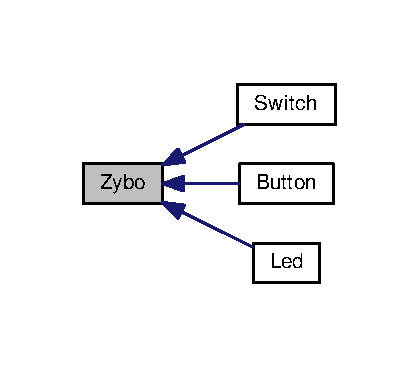
\includegraphics[width=201pt]{group___zybo}
\end{center}
\end{figure}
\subsection*{Moduli}
\begin{DoxyCompactItemize}
\item 
\hyperlink{group___button}{Button}
\item 
\hyperlink{group___led}{Led}
\item 
\hyperlink{group___switch}{Switch}
\end{DoxyCompactItemize}


\subsection{Descrizione dettagliata}

\hypertarget{group___button}{\section{Button}
\label{group___button}\index{Button@{Button}}
}
Diagramma di collaborazione per Button\+:\nopagebreak
\begin{figure}[H]
\begin{center}
\leavevmode
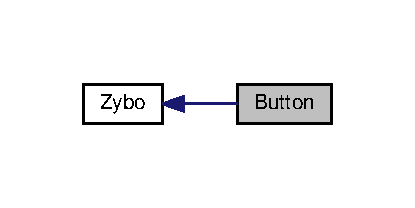
\includegraphics[width=199pt]{group___button}
\end{center}
\end{figure}
\subsection*{Strutture dati}
\begin{DoxyCompactItemize}
\item 
struct \hyperlink{struct_zybo_button__t}{Zybo\+Button\+\_\+t}
\begin{DoxyCompactList}\small\item\em Struttura opaca che astrae l'insieme dei button presenti sulla board Digilent Zybo;. \end{DoxyCompactList}\end{DoxyCompactItemize}
\subsection*{Definizioni}
\begin{DoxyCompactItemize}
\item 
\#define \hyperlink{group___button_ga5f85cbc14732f1d83faa75500b67defa}{Zybo\+Button}(i)~((uint32\+\_\+t)(1$<$$<$i))
\begin{DoxyCompactList}\small\item\em Metodo alternativo per la specifica di uno dei button presenti sulla board Digilent Zybo. \end{DoxyCompactList}\item 
\#define \hyperlink{group___button_ga8960eefa6a431f50d4fe2a2f8063da3f}{Zybo\+Button\+\_\+\+Debounce\+Wait}~50
\begin{DoxyCompactList}\small\item\em Tempo di attesa (in millisecondi) usato per prevenire il fenomeno del bouncing. Il valore di default è 50, determinato empiricamente. Puo' essere modificato a piacimento cambiando il valore alla macro seguente. \end{DoxyCompactList}\end{DoxyCompactItemize}
\subsection*{Tipi enumerati (enum)}
\begin{DoxyCompactItemize}
\item 
enum \hyperlink{group___button_ga4d26a5f6cad606de534ba034e0ba42dd}{Zybo\+Button\+\_\+mask\+\_\+t} \{ \hyperlink{group___button_gga4d26a5f6cad606de534ba034e0ba42ddaabede392be8cae14b8a070a804c754e8}{Zybo\+Button3} = 0x8, 
\hyperlink{group___button_gga4d26a5f6cad606de534ba034e0ba42dda2aa888c8f01ac8a79013e5ebc9eef609}{Zybo\+Button2} = 0x4, 
\hyperlink{group___button_gga4d26a5f6cad606de534ba034e0ba42dda29c35ef3133898c050f675a60de66dd7}{Zybo\+Button1} = 0x2, 
\hyperlink{group___button_gga4d26a5f6cad606de534ba034e0ba42dda2f821ce9661687aefb0ec4de65911570}{Zybo\+Button0} = 0x1
 \}
\begin{DoxyCompactList}\small\item\em Maschere di selezione dei Push\+Button. \end{DoxyCompactList}\item 
enum \hyperlink{group___button_ga85c290bfa232cab213e69200bf78e06a}{Zybo\+Button\+\_\+status\+\_\+t} \{ \hyperlink{group___button_gga85c290bfa232cab213e69200bf78e06aacd110f28912806bcec929721e8737399}{Zybo\+Button\+\_\+off}, 
\hyperlink{group___button_gga85c290bfa232cab213e69200bf78e06aa49bf4a6902270f28bc6a1146fbd1b1fe}{Zybo\+Button\+\_\+on}
 \}
\begin{DoxyCompactList}\small\item\em Status di attivo/inattivo dei Push\+Button. \end{DoxyCompactList}\end{DoxyCompactItemize}
\subsection*{Funzioni}
\begin{DoxyCompactItemize}
\item 
void \hyperlink{group___button_gaa40462223af93b0f5bdf2932400fe2a5}{Zybo\+Button\+\_\+init} (\hyperlink{struct_zybo_button__t}{Zybo\+Button\+\_\+t} $\ast$buttons, \hyperlink{struct_g_p_i_o__t}{G\+P\+I\+O\+\_\+t} $\ast$gpio, \hyperlink{group___g_p_i_o_ga6d5aef8a8a54ee2f602d47252ff66595}{G\+P\+I\+O\+\_\+mask} Button3\+\_\+pin, \hyperlink{group___g_p_i_o_ga6d5aef8a8a54ee2f602d47252ff66595}{G\+P\+I\+O\+\_\+mask} Button2\+\_\+pin, \hyperlink{group___g_p_i_o_ga6d5aef8a8a54ee2f602d47252ff66595}{G\+P\+I\+O\+\_\+mask} Button1\+\_\+pin, \hyperlink{group___g_p_i_o_ga6d5aef8a8a54ee2f602d47252ff66595}{G\+P\+I\+O\+\_\+mask} Button0\+\_\+pin)
\begin{DoxyCompactList}\small\item\em Inizializza un oggetto di tipo \hyperlink{struct_zybo_button__t}{Zybo\+Button\+\_\+t}. \end{DoxyCompactList}\item 
void \hyperlink{group___button_gaca30e81084e746785e395f79e9678e9a}{Zybo\+Button\+\_\+wait\+While\+Idle} (\hyperlink{struct_zybo_button__t}{Zybo\+Button\+\_\+t} $\ast$buttons)
\begin{DoxyCompactList}\small\item\em Permettere di mettere il programma in attesa attiva finche' i button restano inattivi;. \end{DoxyCompactList}\item 
void \hyperlink{group___button_ga3840edf011b5bad6302b7efc9c6326fe}{Zybo\+Button\+\_\+wait\+While\+Busy} (\hyperlink{struct_zybo_button__t}{Zybo\+Button\+\_\+t} $\ast$buttons)
\begin{DoxyCompactList}\small\item\em Permettere di mettere il programma in attesa attiva finche' i button restano attivi;. \end{DoxyCompactList}\item 
\hyperlink{group___button_ga85c290bfa232cab213e69200bf78e06a}{Zybo\+Button\+\_\+status\+\_\+t} \hyperlink{group___button_ga75407539e8ba0ad3ea142496219cd083}{Zybo\+Button\+\_\+get\+Status} (\hyperlink{struct_zybo_button__t}{Zybo\+Button\+\_\+t} $\ast$buttons, \hyperlink{group___button_ga4d26a5f6cad606de534ba034e0ba42dd}{Zybo\+Button\+\_\+mask\+\_\+t} mask)
\begin{DoxyCompactList}\small\item\em Permette la lettura dello stato dei button presenti sulla board. \end{DoxyCompactList}\end{DoxyCompactItemize}


\subsection{Descrizione dettagliata}


\subsection{Documentazione delle definizioni}
\hypertarget{group___button_ga5f85cbc14732f1d83faa75500b67defa}{\index{Button@{Button}!Zybo\+Button@{Zybo\+Button}}
\index{Zybo\+Button@{Zybo\+Button}!Button@{Button}}
\subsubsection[{Zybo\+Button}]{\setlength{\rightskip}{0pt plus 5cm}\#define Zybo\+Button(
\begin{DoxyParamCaption}
\item[{}]{i}
\end{DoxyParamCaption}
)~((uint32\+\_\+t)(1$<$$<$i))}}\label{group___button_ga5f85cbc14732f1d83faa75500b67defa}


Metodo alternativo per la specifica di uno dei button presenti sulla board Digilent Zybo. 


\begin{DoxyParams}{Parametri}
{\em i} & indice del button da selezionare, da 0 a 3 \\
\hline
\end{DoxyParams}
\begin{DoxyReturn}{Restituisce}
maschera di selezione del button i-\/esimo 
\end{DoxyReturn}
\hypertarget{group___button_ga8960eefa6a431f50d4fe2a2f8063da3f}{\index{Button@{Button}!Zybo\+Button\+\_\+\+Debounce\+Wait@{Zybo\+Button\+\_\+\+Debounce\+Wait}}
\index{Zybo\+Button\+\_\+\+Debounce\+Wait@{Zybo\+Button\+\_\+\+Debounce\+Wait}!Button@{Button}}
\subsubsection[{Zybo\+Button\+\_\+\+Debounce\+Wait}]{\setlength{\rightskip}{0pt plus 5cm}\#define Zybo\+Button\+\_\+\+Debounce\+Wait~50}}\label{group___button_ga8960eefa6a431f50d4fe2a2f8063da3f}


Tempo di attesa (in millisecondi) usato per prevenire il fenomeno del bouncing. Il valore di default è 50, determinato empiricamente. Puo' essere modificato a piacimento cambiando il valore alla macro seguente. 



\subsection{Documentazione dei tipi enumerati}
\hypertarget{group___button_ga4d26a5f6cad606de534ba034e0ba42dd}{\index{Button@{Button}!Zybo\+Button\+\_\+mask\+\_\+t@{Zybo\+Button\+\_\+mask\+\_\+t}}
\index{Zybo\+Button\+\_\+mask\+\_\+t@{Zybo\+Button\+\_\+mask\+\_\+t}!Button@{Button}}
\subsubsection[{Zybo\+Button\+\_\+mask\+\_\+t}]{\setlength{\rightskip}{0pt plus 5cm}enum {\bf Zybo\+Button\+\_\+mask\+\_\+t}}}\label{group___button_ga4d26a5f6cad606de534ba034e0ba42dd}


Maschere di selezione dei Push\+Button. 

\begin{Desc}
\item[Valori del tipo enumerato]\par
\begin{description}
\index{Zybo\+Button3@{Zybo\+Button3}!Button@{Button}}\index{Button@{Button}!Zybo\+Button3@{Zybo\+Button3}}\item[{\em 
\hypertarget{group___button_gga4d26a5f6cad606de534ba034e0ba42ddaabede392be8cae14b8a070a804c754e8}{Zybo\+Button3}\label{group___button_gga4d26a5f6cad606de534ba034e0ba42ddaabede392be8cae14b8a070a804c754e8}
}]Zybo\+Button3, seleziona il button 3 sulla board Digilent Zybo;. \index{Zybo\+Button2@{Zybo\+Button2}!Button@{Button}}\index{Button@{Button}!Zybo\+Button2@{Zybo\+Button2}}\item[{\em 
\hypertarget{group___button_gga4d26a5f6cad606de534ba034e0ba42dda2aa888c8f01ac8a79013e5ebc9eef609}{Zybo\+Button2}\label{group___button_gga4d26a5f6cad606de534ba034e0ba42dda2aa888c8f01ac8a79013e5ebc9eef609}
}]Zybo\+Button2, seleziona il button 2 sulla board Digilent Zybo;. \index{Zybo\+Button1@{Zybo\+Button1}!Button@{Button}}\index{Button@{Button}!Zybo\+Button1@{Zybo\+Button1}}\item[{\em 
\hypertarget{group___button_gga4d26a5f6cad606de534ba034e0ba42dda29c35ef3133898c050f675a60de66dd7}{Zybo\+Button1}\label{group___button_gga4d26a5f6cad606de534ba034e0ba42dda29c35ef3133898c050f675a60de66dd7}
}]Zybo\+Button1, seleziona il button 1 sulla board Digilent Zybo;. \index{Zybo\+Button0@{Zybo\+Button0}!Button@{Button}}\index{Button@{Button}!Zybo\+Button0@{Zybo\+Button0}}\item[{\em 
\hypertarget{group___button_gga4d26a5f6cad606de534ba034e0ba42dda2f821ce9661687aefb0ec4de65911570}{Zybo\+Button0}\label{group___button_gga4d26a5f6cad606de534ba034e0ba42dda2f821ce9661687aefb0ec4de65911570}
}]Zybo\+Button0, seleziona il button 0 sulla board Digilent Zybo;. \end{description}
\end{Desc}
\hypertarget{group___button_ga85c290bfa232cab213e69200bf78e06a}{\index{Button@{Button}!Zybo\+Button\+\_\+status\+\_\+t@{Zybo\+Button\+\_\+status\+\_\+t}}
\index{Zybo\+Button\+\_\+status\+\_\+t@{Zybo\+Button\+\_\+status\+\_\+t}!Button@{Button}}
\subsubsection[{Zybo\+Button\+\_\+status\+\_\+t}]{\setlength{\rightskip}{0pt plus 5cm}enum {\bf Zybo\+Button\+\_\+status\+\_\+t}}}\label{group___button_ga85c290bfa232cab213e69200bf78e06a}


Status di attivo/inattivo dei Push\+Button. 

\begin{Desc}
\item[Valori del tipo enumerato]\par
\begin{description}
\index{Zybo\+Button\+\_\+off@{Zybo\+Button\+\_\+off}!Button@{Button}}\index{Button@{Button}!Zybo\+Button\+\_\+off@{Zybo\+Button\+\_\+off}}\item[{\em 
\hypertarget{group___button_gga85c290bfa232cab213e69200bf78e06aacd110f28912806bcec929721e8737399}{Zybo\+Button\+\_\+off}\label{group___button_gga85c290bfa232cab213e69200bf78e06aacd110f28912806bcec929721e8737399}
}]Zybo\+Button\+\_\+off, corrisponde al valore logico '0', indica che un pushbutton e' inattivo;. \index{Zybo\+Button\+\_\+on@{Zybo\+Button\+\_\+on}!Button@{Button}}\index{Button@{Button}!Zybo\+Button\+\_\+on@{Zybo\+Button\+\_\+on}}\item[{\em 
\hypertarget{group___button_gga85c290bfa232cab213e69200bf78e06aa49bf4a6902270f28bc6a1146fbd1b1fe}{Zybo\+Button\+\_\+on}\label{group___button_gga85c290bfa232cab213e69200bf78e06aa49bf4a6902270f28bc6a1146fbd1b1fe}
}]Zybo\+Button\+\_\+on, corrisponde al valore logico '1', indica che un pushbutton e' attivo;. \end{description}
\end{Desc}


\subsection{Documentazione delle funzioni}
\hypertarget{group___button_ga75407539e8ba0ad3ea142496219cd083}{\index{Button@{Button}!Zybo\+Button\+\_\+get\+Status@{Zybo\+Button\+\_\+get\+Status}}
\index{Zybo\+Button\+\_\+get\+Status@{Zybo\+Button\+\_\+get\+Status}!Button@{Button}}
\subsubsection[{Zybo\+Button\+\_\+get\+Status}]{\setlength{\rightskip}{0pt plus 5cm}{\bf Zybo\+Button\+\_\+status\+\_\+t} Zybo\+Button\+\_\+get\+Status (
\begin{DoxyParamCaption}
\item[{{\bf Zybo\+Button\+\_\+t} $\ast$}]{buttons, }
\item[{{\bf Zybo\+Button\+\_\+mask\+\_\+t}}]{mask}
\end{DoxyParamCaption}
)}}\label{group___button_ga75407539e8ba0ad3ea142496219cd083}


Permette la lettura dello stato dei button presenti sulla board. 


\begin{DoxyParams}[1]{Parametri}
\mbox{\tt in}  & {\em buttons} & puntatore a struttura \hyperlink{struct_zybo_button__t}{Zybo\+Button\+\_\+t}, che astrae l'insieme dei button presenti sulla board Digilent Zybo; \\
\hline
\mbox{\tt in}  & {\em mask} & maschera di selezione dei button, quelli non selezionati non vengono tenuti in considerazione\\
\hline
\end{DoxyParams}
\begin{DoxyReturn}{Restituisce}
status status dei button 
\end{DoxyReturn}

\begin{DoxyRetVals}{Valori di ritorno}
{\em Zybo\+Button\+\_\+on} & se uno dei button selezionati e' attivo; \\
\hline
{\em Zybo\+Button\+\_\+off} & altrimenti\\
\hline
\end{DoxyRetVals}

\begin{DoxyCode}
1 ZyboButton\_status\_t button\_status = ZyboButton\_getStatus(&buttons, ZyboButton3);                // leggo lo
       stato ddi button 3
2 ZyboLed\_status\_t led\_status = (button\_status == ZyboButton\_on ? ZyboLed\_on : ZyboLed\_off);  // se lo stato
       e' attivo accendo il led 3
3 ZyboLed\_setStatus(&leds, ZyboLed3, led\_status);                                             //
       accendo/spengo led 3
\end{DoxyCode}


\begin{DoxyWarning}{Avvertimento}
Usa la macro assert per verificare che\+:
\begin{DoxyItemize}
\item buttons non sia un puntatore nullo;
\item buttons-\/$>$gpio non sia un puntatore nullo 
\end{DoxyItemize}
\end{DoxyWarning}
\hypertarget{group___button_gaa40462223af93b0f5bdf2932400fe2a5}{\index{Button@{Button}!Zybo\+Button\+\_\+init@{Zybo\+Button\+\_\+init}}
\index{Zybo\+Button\+\_\+init@{Zybo\+Button\+\_\+init}!Button@{Button}}
\subsubsection[{Zybo\+Button\+\_\+init}]{\setlength{\rightskip}{0pt plus 5cm}void Zybo\+Button\+\_\+init (
\begin{DoxyParamCaption}
\item[{{\bf Zybo\+Button\+\_\+t} $\ast$}]{buttons, }
\item[{{\bf G\+P\+I\+O\+\_\+t} $\ast$}]{gpio, }
\item[{{\bf G\+P\+I\+O\+\_\+mask}}]{Button3\+\_\+pin, }
\item[{{\bf G\+P\+I\+O\+\_\+mask}}]{Button2\+\_\+pin, }
\item[{{\bf G\+P\+I\+O\+\_\+mask}}]{Button1\+\_\+pin, }
\item[{{\bf G\+P\+I\+O\+\_\+mask}}]{Button0\+\_\+pin}
\end{DoxyParamCaption}
)}}\label{group___button_gaa40462223af93b0f5bdf2932400fe2a5}


Inizializza un oggetto di tipo \hyperlink{struct_zybo_button__t}{Zybo\+Button\+\_\+t}. 


\begin{DoxyParams}[1]{Parametri}
\mbox{\tt in,out}  & {\em buttons} & puntatore a struttura \hyperlink{struct_zybo_button__t}{Zybo\+Button\+\_\+t}, che astrae l'insieme dei button presenti sulla board Digilent Zybo; \\
\hline
\mbox{\tt in}  & {\em gpio} & puntatore a struttura \hyperlink{struct_g_p_i_o__t}{G\+P\+I\+O\+\_\+t}, che astrae un device G\+P\+I\+O; non viene inizializzato dalla funziona, sara' necessario inizializzarlo preventivamente; si faccia riferimento all'esempio riportato di seguito \\
\hline
\mbox{\tt in}  & {\em Button3\+\_\+pin} & pin del device G\+P\+I\+O a cui e' associato il button 3 della board Digilent Zybo; \\
\hline
\mbox{\tt in}  & {\em Button2\+\_\+pin} & pin del device G\+P\+I\+O a cui e' associato il button 2 della board Digilent Zybo; \\
\hline
\mbox{\tt in}  & {\em Button1\+\_\+pin} & pin del device G\+P\+I\+O a cui e' associato il button 1 della board Digilent Zybo; \\
\hline
\mbox{\tt in}  & {\em Button0\+\_\+pin} & pin del device G\+P\+I\+O a cui e' associato il button 0 della board Digilent Zybo;\\
\hline
\end{DoxyParams}

\begin{DoxyCode}
1 GPIO\_t gpioButton;
2 GPIO\_init(&gpioButton, XPAR\_MYGPIO\_1\_S00\_AXI\_BASEADDR, 4, 0, 4, 8);
3 ZyboButton\_t buttons;
4 ZyboButton\_init(&buttons, &gpioButton, GPIO\_pin3, GPIO\_pin2, GPIO\_pin1, GPIO\_pin0);
\end{DoxyCode}


\begin{DoxyWarning}{Avvertimento}
Usa la macro assert per verificare che\+:
\begin{DoxyItemize}
\item buttons non sia un puntatore nullo;
\item gpio non sia un puntatore nullo
\item Button\+N\+\_\+pin siano tutti pin differenti 
\end{DoxyItemize}
\end{DoxyWarning}
\hypertarget{group___button_ga3840edf011b5bad6302b7efc9c6326fe}{\index{Button@{Button}!Zybo\+Button\+\_\+wait\+While\+Busy@{Zybo\+Button\+\_\+wait\+While\+Busy}}
\index{Zybo\+Button\+\_\+wait\+While\+Busy@{Zybo\+Button\+\_\+wait\+While\+Busy}!Button@{Button}}
\subsubsection[{Zybo\+Button\+\_\+wait\+While\+Busy}]{\setlength{\rightskip}{0pt plus 5cm}void Zybo\+Button\+\_\+wait\+While\+Busy (
\begin{DoxyParamCaption}
\item[{{\bf Zybo\+Button\+\_\+t} $\ast$}]{buttons}
\end{DoxyParamCaption}
)}}\label{group___button_ga3840edf011b5bad6302b7efc9c6326fe}


Permettere di mettere il programma in attesa attiva finche' i button restano attivi;. 

\begin{DoxyWarning}{Avvertimento}
La funzione integra le funzionalita' di debouncing. Il tempo di attesa e' determinato sulla base del valore della macro Zybo\+Button\+\_\+\+Debounce\+Wait. Per l'attesa viene usata la funzione usleep() di stdlib.
\end{DoxyWarning}

\begin{DoxyParams}[1]{Parametri}
\mbox{\tt in}  & {\em buttons} & puntatore a struttura \hyperlink{struct_zybo_button__t}{Zybo\+Button\+\_\+t}, che astrae l'insieme dei button presenti sulla board Digilent Zybo;\\
\hline
\end{DoxyParams}

\begin{DoxyCode}
1 ZyboButton\_waitWhileIdle(&buttons);
2 ZyboButton\_status\_t button3\_status = ZyboButton\_getStatus(&buttons, ZyboButton3);               // leggo lo
       stato ddi button 3
3 ZyboButton\_status\_t button2\_status = ZyboButton\_getStatus(&buttons, ZyboButton2);               // leggo lo
       stato ddi button 2
4 ZyboButton\_status\_t button1\_status = ZyboButton\_getStatus(&buttons, ZyboButton1);               // leggo lo
       stato ddi button 1
5 ZyboButton\_status\_t button0\_status = ZyboButton\_getStatus(&buttons, ZyboButton0);               // leggo lo
       stato ddi button 0
6 ZyboButton\_waitWhileBusy(&buttons);
\end{DoxyCode}


\begin{DoxyWarning}{Avvertimento}
Usa la macro assert per verificare che\+:
\begin{DoxyItemize}
\item buttons non sia un puntatore nullo;
\item buttons-\/$>$gpio non sia un puntatore nullo 
\end{DoxyItemize}
\end{DoxyWarning}
\hypertarget{group___button_gaca30e81084e746785e395f79e9678e9a}{\index{Button@{Button}!Zybo\+Button\+\_\+wait\+While\+Idle@{Zybo\+Button\+\_\+wait\+While\+Idle}}
\index{Zybo\+Button\+\_\+wait\+While\+Idle@{Zybo\+Button\+\_\+wait\+While\+Idle}!Button@{Button}}
\subsubsection[{Zybo\+Button\+\_\+wait\+While\+Idle}]{\setlength{\rightskip}{0pt plus 5cm}void Zybo\+Button\+\_\+wait\+While\+Idle (
\begin{DoxyParamCaption}
\item[{{\bf Zybo\+Button\+\_\+t} $\ast$}]{buttons}
\end{DoxyParamCaption}
)}}\label{group___button_gaca30e81084e746785e395f79e9678e9a}


Permettere di mettere il programma in attesa attiva finche' i button restano inattivi;. 

\begin{DoxyWarning}{Avvertimento}
La funzione integra le funzionalita' di debouncing. Il tempo di attesa e' determinato sulla base del valore della macro Zybo\+Button\+\_\+\+Debounce\+Wait. Per l'attesa viene usata la funzione usleep() di stdlib.
\end{DoxyWarning}

\begin{DoxyParams}[1]{Parametri}
\mbox{\tt in}  & {\em buttons} & puntatore a struttura \hyperlink{struct_zybo_button__t}{Zybo\+Button\+\_\+t}, che astrae l'insieme dei button presenti sulla board Digilent Zybo;\\
\hline
\end{DoxyParams}

\begin{DoxyCode}
1 ZyboButton\_waitWhileIdle(&buttons);
2 ZyboButton\_status\_t button3\_status = ZyboButton\_getStatus(&buttons, ZyboButton3);               // leggo lo
       stato ddi button 3
3 ZyboButton\_status\_t button2\_status = ZyboButton\_getStatus(&buttons, ZyboButton2);               // leggo lo
       stato ddi button 2
4 ZyboButton\_status\_t button1\_status = ZyboButton\_getStatus(&buttons, ZyboButton1);               // leggo lo
       stato ddi button 1
5 ZyboButton\_status\_t button0\_status = ZyboButton\_getStatus(&buttons, ZyboButton0);               // leggo lo
       stato ddi button 0
6 ZyboButton\_waitWhileBusy(&buttons);
\end{DoxyCode}


\begin{DoxyWarning}{Avvertimento}
Usa la macro assert per verificare che\+:
\begin{DoxyItemize}
\item buttons non sia un puntatore nullo;
\item buttons-\/$>$gpio non sia un puntatore nullo 
\end{DoxyItemize}
\end{DoxyWarning}

\hypertarget{group___led}{\section{Led}
\label{group___led}\index{Led@{Led}}
}
Diagramma di collaborazione per Led\+:\nopagebreak
\begin{figure}[H]
\begin{center}
\leavevmode
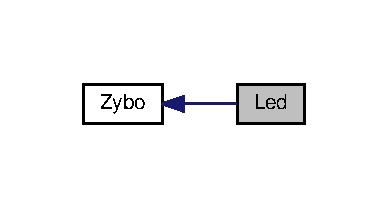
\includegraphics[width=186pt]{group___led}
\end{center}
\end{figure}
\subsection*{Strutture dati}
\begin{DoxyCompactItemize}
\item 
struct \hyperlink{struct_zybo_led__t}{Zybo\+Led\+\_\+t}
\begin{DoxyCompactList}\small\item\em Struttura opaca che astrae l'insieme dei Led presenti sulla board Digilent Zybo;. \end{DoxyCompactList}\end{DoxyCompactItemize}
\subsection*{Definizioni}
\begin{DoxyCompactItemize}
\item 
\#define \hyperlink{group___led_ga50ab39fed34dc3aaf53cdfd67d8ba25d}{Zybo\+Led}(i)~((uint32\+\_\+t)(1$<$$<$(i)))
\begin{DoxyCompactList}\small\item\em Metodo alternativo per la specifica di uno dei led presenti sulla board Digilent Zybo. \end{DoxyCompactList}\end{DoxyCompactItemize}
\subsection*{Tipi enumerati (enum)}
\begin{DoxyCompactItemize}
\item 
enum \hyperlink{group___led_gad11701cccac394f7e1f90de8f85695f3}{Zybo\+Led\+\_\+mask\+\_\+t} \{ \hyperlink{group___led_ggad11701cccac394f7e1f90de8f85695f3adc5edc2adfd899da9f149cb61364b141}{Zybo\+Led3} = 0x8\+U, 
\hyperlink{group___led_ggad11701cccac394f7e1f90de8f85695f3a4fa521f6fce7c4ba77d1d8144e71cdfc}{Zybo\+Led2} = 0x4\+U, 
\hyperlink{group___led_ggad11701cccac394f7e1f90de8f85695f3ad71c06f65dfffcf825d48f287718d9be}{Zybo\+Led1} = 0x2\+U, 
\hyperlink{group___led_ggad11701cccac394f7e1f90de8f85695f3ae1a1e8fa0bf803793ff27004884b85fe}{Zybo\+Led0} = 0x1\+U
 \}
\begin{DoxyCompactList}\small\item\em Maschere di selezione dei led. \end{DoxyCompactList}\item 
enum \hyperlink{group___led_ga3dcb274f22e577705c49944b8d1f4b12}{Zybo\+Led\+\_\+status\+\_\+t} \{ \hyperlink{group___led_gga3dcb274f22e577705c49944b8d1f4b12a9679f1c302afdb51915a2331b4ec92f3}{Zybo\+Led\+\_\+off}, 
\hyperlink{group___led_gga3dcb274f22e577705c49944b8d1f4b12aafcf0ae16a6edec807c06bb0a99f7e8b}{Zybo\+Led\+\_\+on}
 \}
\begin{DoxyCompactList}\small\item\em Status di accensione/spegnimento dei led. \end{DoxyCompactList}\end{DoxyCompactItemize}
\subsection*{Funzioni}
\begin{DoxyCompactItemize}
\item 
void \hyperlink{group___led_ga51bccd37e6ae8cd32e2c50c60a5e83cc}{Zybo\+Led\+\_\+init} (\hyperlink{struct_zybo_led__t}{Zybo\+Led\+\_\+t} $\ast$leds, \hyperlink{structmy_g_p_i_o__t}{my\+G\+P\+I\+O\+\_\+t} $\ast$gpio, \hyperlink{group__my_g_p_i_o_ga402a0d20afc0cb7c25554b8b023f4253}{my\+G\+P\+I\+O\+\_\+mask} Led3\+\_\+pin, \hyperlink{group__my_g_p_i_o_ga402a0d20afc0cb7c25554b8b023f4253}{my\+G\+P\+I\+O\+\_\+mask} Led2\+\_\+pin, \hyperlink{group__my_g_p_i_o_ga402a0d20afc0cb7c25554b8b023f4253}{my\+G\+P\+I\+O\+\_\+mask} Led1\+\_\+pin, \hyperlink{group__my_g_p_i_o_ga402a0d20afc0cb7c25554b8b023f4253}{my\+G\+P\+I\+O\+\_\+mask} Led0\+\_\+pin)
\begin{DoxyCompactList}\small\item\em Inizializza un oggetto di tipo \hyperlink{struct_zybo_led__t}{Zybo\+Led\+\_\+t}. \end{DoxyCompactList}\item 
void \hyperlink{group___led_gacf5c2b0328c4bdf2d796397fc4510c69}{Zybo\+Led\+\_\+set\+Status} (\hyperlink{struct_zybo_led__t}{Zybo\+Led\+\_\+t} $\ast$leds, \hyperlink{group___led_gad11701cccac394f7e1f90de8f85695f3}{Zybo\+Led\+\_\+mask\+\_\+t} mask, \hyperlink{group___led_ga3dcb274f22e577705c49944b8d1f4b12}{Zybo\+Led\+\_\+status\+\_\+t} status)
\begin{DoxyCompactList}\small\item\em Permette di accendere/spegnere i Led sulla board. \end{DoxyCompactList}\item 
void \hyperlink{group___led_ga20ddd78a98b4c0123c5b964aa0a59046}{Zybo\+Led\+\_\+toggle} (\hyperlink{struct_zybo_led__t}{Zybo\+Led\+\_\+t} $\ast$leds, \hyperlink{group___led_gad11701cccac394f7e1f90de8f85695f3}{Zybo\+Led\+\_\+mask\+\_\+t} mask)
\begin{DoxyCompactList}\small\item\em Permette di accendere/spegnere i Led sulla board, invertendone il valore. \end{DoxyCompactList}\end{DoxyCompactItemize}


\subsection{Descrizione dettagliata}


\subsection{Documentazione delle definizioni}
\hypertarget{group___led_ga50ab39fed34dc3aaf53cdfd67d8ba25d}{\index{Led@{Led}!Zybo\+Led@{Zybo\+Led}}
\index{Zybo\+Led@{Zybo\+Led}!Led@{Led}}
\subsubsection[{Zybo\+Led}]{\setlength{\rightskip}{0pt plus 5cm}\#define Zybo\+Led(
\begin{DoxyParamCaption}
\item[{}]{i}
\end{DoxyParamCaption}
)~((uint32\+\_\+t)(1$<$$<$(i)))}}\label{group___led_ga50ab39fed34dc3aaf53cdfd67d8ba25d}


Metodo alternativo per la specifica di uno dei led presenti sulla board Digilent Zybo. 


\begin{DoxyParams}[1]{Parametri}
\mbox{\tt in}  & {\em i} & indice del led da selezionare, da 0 a 3 \\
\hline
\end{DoxyParams}
\begin{DoxyReturn}{Restituisce}
maschera di selezione del led i-\/esimo 
\end{DoxyReturn}


\subsection{Documentazione dei tipi enumerati}
\hypertarget{group___led_gad11701cccac394f7e1f90de8f85695f3}{\index{Led@{Led}!Zybo\+Led\+\_\+mask\+\_\+t@{Zybo\+Led\+\_\+mask\+\_\+t}}
\index{Zybo\+Led\+\_\+mask\+\_\+t@{Zybo\+Led\+\_\+mask\+\_\+t}!Led@{Led}}
\subsubsection[{Zybo\+Led\+\_\+mask\+\_\+t}]{\setlength{\rightskip}{0pt plus 5cm}enum {\bf Zybo\+Led\+\_\+mask\+\_\+t}}}\label{group___led_gad11701cccac394f7e1f90de8f85695f3}


Maschere di selezione dei led. 

\begin{Desc}
\item[Valori del tipo enumerato]\par
\begin{description}
\index{Zybo\+Led3@{Zybo\+Led3}!Led@{Led}}\index{Led@{Led}!Zybo\+Led3@{Zybo\+Led3}}\item[{\em 
\hypertarget{group___led_ggad11701cccac394f7e1f90de8f85695f3adc5edc2adfd899da9f149cb61364b141}{Zybo\+Led3}\label{group___led_ggad11701cccac394f7e1f90de8f85695f3adc5edc2adfd899da9f149cb61364b141}
}]Zybo\+Led3, seleziona il led 3 sulla board Digilent Zybo;. \index{Zybo\+Led2@{Zybo\+Led2}!Led@{Led}}\index{Led@{Led}!Zybo\+Led2@{Zybo\+Led2}}\item[{\em 
\hypertarget{group___led_ggad11701cccac394f7e1f90de8f85695f3a4fa521f6fce7c4ba77d1d8144e71cdfc}{Zybo\+Led2}\label{group___led_ggad11701cccac394f7e1f90de8f85695f3a4fa521f6fce7c4ba77d1d8144e71cdfc}
}]Zybo\+Led2, seleziona il led 2 sulla board Digilent Zybo;. \index{Zybo\+Led1@{Zybo\+Led1}!Led@{Led}}\index{Led@{Led}!Zybo\+Led1@{Zybo\+Led1}}\item[{\em 
\hypertarget{group___led_ggad11701cccac394f7e1f90de8f85695f3ad71c06f65dfffcf825d48f287718d9be}{Zybo\+Led1}\label{group___led_ggad11701cccac394f7e1f90de8f85695f3ad71c06f65dfffcf825d48f287718d9be}
}]Zybo\+Led1, seleziona il led 1 sulla board Digilent Zybo;. \index{Zybo\+Led0@{Zybo\+Led0}!Led@{Led}}\index{Led@{Led}!Zybo\+Led0@{Zybo\+Led0}}\item[{\em 
\hypertarget{group___led_ggad11701cccac394f7e1f90de8f85695f3ae1a1e8fa0bf803793ff27004884b85fe}{Zybo\+Led0}\label{group___led_ggad11701cccac394f7e1f90de8f85695f3ae1a1e8fa0bf803793ff27004884b85fe}
}]Zybo\+Led0, seleziona il led 0 sulla board Digilent Zybo;. \end{description}
\end{Desc}
\hypertarget{group___led_ga3dcb274f22e577705c49944b8d1f4b12}{\index{Led@{Led}!Zybo\+Led\+\_\+status\+\_\+t@{Zybo\+Led\+\_\+status\+\_\+t}}
\index{Zybo\+Led\+\_\+status\+\_\+t@{Zybo\+Led\+\_\+status\+\_\+t}!Led@{Led}}
\subsubsection[{Zybo\+Led\+\_\+status\+\_\+t}]{\setlength{\rightskip}{0pt plus 5cm}enum {\bf Zybo\+Led\+\_\+status\+\_\+t}}}\label{group___led_ga3dcb274f22e577705c49944b8d1f4b12}


Status di accensione/spegnimento dei led. 

\begin{Desc}
\item[Valori del tipo enumerato]\par
\begin{description}
\index{Zybo\+Led\+\_\+off@{Zybo\+Led\+\_\+off}!Led@{Led}}\index{Led@{Led}!Zybo\+Led\+\_\+off@{Zybo\+Led\+\_\+off}}\item[{\em 
\hypertarget{group___led_gga3dcb274f22e577705c49944b8d1f4b12a9679f1c302afdb51915a2331b4ec92f3}{Zybo\+Led\+\_\+off}\label{group___led_gga3dcb274f22e577705c49944b8d1f4b12a9679f1c302afdb51915a2331b4ec92f3}
}]Zybo\+Led\+\_\+off, corrisponde al valore logico '0', per lo spegnimento dei Led. \index{Zybo\+Led\+\_\+on@{Zybo\+Led\+\_\+on}!Led@{Led}}\index{Led@{Led}!Zybo\+Led\+\_\+on@{Zybo\+Led\+\_\+on}}\item[{\em 
\hypertarget{group___led_gga3dcb274f22e577705c49944b8d1f4b12aafcf0ae16a6edec807c06bb0a99f7e8b}{Zybo\+Led\+\_\+on}\label{group___led_gga3dcb274f22e577705c49944b8d1f4b12aafcf0ae16a6edec807c06bb0a99f7e8b}
}]Zybo\+Led\+\_\+on, corrisponde al valore logico '1', per l'accensione dei Led. \end{description}
\end{Desc}


\subsection{Documentazione delle funzioni}
\hypertarget{group___led_ga51bccd37e6ae8cd32e2c50c60a5e83cc}{\index{Led@{Led}!Zybo\+Led\+\_\+init@{Zybo\+Led\+\_\+init}}
\index{Zybo\+Led\+\_\+init@{Zybo\+Led\+\_\+init}!Led@{Led}}
\subsubsection[{Zybo\+Led\+\_\+init}]{\setlength{\rightskip}{0pt plus 5cm}void Zybo\+Led\+\_\+init (
\begin{DoxyParamCaption}
\item[{{\bf Zybo\+Led\+\_\+t} $\ast$}]{leds, }
\item[{{\bf my\+G\+P\+I\+O\+\_\+t} $\ast$}]{gpio, }
\item[{{\bf my\+G\+P\+I\+O\+\_\+mask}}]{Led3\+\_\+pin, }
\item[{{\bf my\+G\+P\+I\+O\+\_\+mask}}]{Led2\+\_\+pin, }
\item[{{\bf my\+G\+P\+I\+O\+\_\+mask}}]{Led1\+\_\+pin, }
\item[{{\bf my\+G\+P\+I\+O\+\_\+mask}}]{Led0\+\_\+pin}
\end{DoxyParamCaption}
)}}\label{group___led_ga51bccd37e6ae8cd32e2c50c60a5e83cc}


Inizializza un oggetto di tipo \hyperlink{struct_zybo_led__t}{Zybo\+Led\+\_\+t}. 

Inizializza un oggetto di tipo \hyperlink{struct_zybo_led__t}{Zybo\+Led\+\_\+t}, che astrae e consente di pilotare i led presenti sulla board Digilent Zybo. Per il pilotaggio viene usato il modulo G\+P\+I\+O ed un puntatore ad una struttura \hyperlink{structmy_g_p_i_o__t}{my\+G\+P\+I\+O\+\_\+t} che lo astrae. Tale struttura non viene inizializzata dalla funzione Zybo\+Led\+\_\+init, per cui sara' necessario inizializzarlo preventivamente. La funzione, pero', si assume l'onere di configurare i pin del device G\+P\+I\+O a cui i led sono connessi.


\begin{DoxyParams}[1]{Parametri}
\mbox{\tt in,out}  & {\em leds} & puntatore a struttura \hyperlink{struct_zybo_led__t}{Zybo\+Led\+\_\+t}, che astrae l'insieme dei Led presenti sulla board Digilent Zybo; \\
\hline
\mbox{\tt in}  & {\em gpio} & puntatore a struttura \hyperlink{structmy_g_p_i_o__t}{my\+G\+P\+I\+O\+\_\+t}, che astrae un device G\+P\+I\+O; la struttura \hyperlink{structmy_g_p_i_o__t}{my\+G\+P\+I\+O\+\_\+t} non viene inizializzata dalla funzione, per cui sara' necessario farlo preventivamente; si faccia riferimento all'esempio riportato di seguito. \\
\hline
\mbox{\tt in}  & {\em Led3\+\_\+pin} & pin del device G\+P\+I\+O a cui e' associato il Led3 della board Digilent Zybo; \\
\hline
\mbox{\tt in}  & {\em Led2\+\_\+pin} & pin del device G\+P\+I\+O a cui e' associato il Led2 della board Digilent Zybo; \\
\hline
\mbox{\tt in}  & {\em Led1\+\_\+pin} & pin del device G\+P\+I\+O a cui e' associato il Led1 della board Digilent Zybo; \\
\hline
\mbox{\tt in}  & {\em Led0\+\_\+pin} & pin del device G\+P\+I\+O a cui e' associato il Led0 della board Digilent Zybo;\\
\hline
\end{DoxyParams}

\begin{DoxyCode}
1 myGPIO\_t gpioLed;
2 GPIO\_init(&gpioLed, XPAR\_MYGPIO\_0\_S00\_AXI\_BASEADDR, 4, 0, 4, 8);                // inizializzazione del
       device GPIO
3 ZyboLed\_t leds;
4 ZyboLed\_init(&leds, &gpioLed, GPIO\_pin3, GPIO\_pin2, GPIO\_pin1, GPIO\_pin0);  // inzializzazione della
       struttura ZyboLed\_t
\end{DoxyCode}


\begin{DoxyWarning}{Avvertimento}
Usa la macro assert per verificare che\+:
\begin{DoxyItemize}
\item leds non sia un puntatore nullo;
\item gpio non sia un puntatore nullo
\item Led\+N\+\_\+pin siano tutti pin differenti 
\end{DoxyItemize}
\end{DoxyWarning}
\hypertarget{group___led_gacf5c2b0328c4bdf2d796397fc4510c69}{\index{Led@{Led}!Zybo\+Led\+\_\+set\+Status@{Zybo\+Led\+\_\+set\+Status}}
\index{Zybo\+Led\+\_\+set\+Status@{Zybo\+Led\+\_\+set\+Status}!Led@{Led}}
\subsubsection[{Zybo\+Led\+\_\+set\+Status}]{\setlength{\rightskip}{0pt plus 5cm}void Zybo\+Led\+\_\+set\+Status (
\begin{DoxyParamCaption}
\item[{{\bf Zybo\+Led\+\_\+t} $\ast$}]{leds, }
\item[{{\bf Zybo\+Led\+\_\+mask\+\_\+t}}]{mask, }
\item[{{\bf Zybo\+Led\+\_\+status\+\_\+t}}]{status}
\end{DoxyParamCaption}
)}}\label{group___led_gacf5c2b0328c4bdf2d796397fc4510c69}


Permette di accendere/spegnere i Led sulla board. 


\begin{DoxyParams}[1]{Parametri}
\mbox{\tt in}  & {\em leds} & puntatore a struttura \hyperlink{struct_zybo_led__t}{Zybo\+Led\+\_\+t}, che astrae l'insieme dei Led presenti sulla board Digilent Zybo; \\
\hline
\mbox{\tt in}  & {\em mask} & maschera di selezione dei led, quelli non selezionati vengono lasciati inalterati \\
\hline
\mbox{\tt in}  & {\em status} & status dei led, Zybo\+Led\+\_\+on per accendere, Zybo\+Led\+\_\+off per spegnere\\
\hline
\end{DoxyParams}

\begin{DoxyCode}
1 ZyboLed\_setStatus(&leds, ZyboLed3 | ZyboLed1, ZyboLed\_on);  // accensione dei Led 3 ed 1
2 ZyboLed\_setStatus(&leds, ZyboLed3 | ZyboLed1, ZyboLed\_off); // spegnimento dei Led 3 ed 1
3 ZyboLed\_setStatus(&leds, ZyboLed2 | ZyboLed0, ZyboLed\_on);  // accendsione dei Led 2 ed 0
4 ZyboLed\_setStatus(&leds, ZyboLed2 | ZyboLed0, ZyboLed\_off); // spegnimento dei Led 2 ed 0
5 ZyboLed\_setStatus(&leds, ZyboLed3 | ZyboLed1 | ZyboLed2 | ZyboLed0, ZyboLed\_on);        // accensone di
       tutti i led
6 ZyboLed\_setStatus(&leds, ZyboLed3 | ZyboLed1 | ZyboLed2 | ZyboLed0, ZyboLed\_off);   // spegnimento di tutti
       i led
\end{DoxyCode}


\begin{DoxyWarning}{Avvertimento}
Usa la macro assert per verificare che\+:
\begin{DoxyItemize}
\item leds non sia un puntatore nullo;
\item leds-\/$>$gpio non sia un puntatore nullo 
\end{DoxyItemize}
\end{DoxyWarning}
\hypertarget{group___led_ga20ddd78a98b4c0123c5b964aa0a59046}{\index{Led@{Led}!Zybo\+Led\+\_\+toggle@{Zybo\+Led\+\_\+toggle}}
\index{Zybo\+Led\+\_\+toggle@{Zybo\+Led\+\_\+toggle}!Led@{Led}}
\subsubsection[{Zybo\+Led\+\_\+toggle}]{\setlength{\rightskip}{0pt plus 5cm}void Zybo\+Led\+\_\+toggle (
\begin{DoxyParamCaption}
\item[{{\bf Zybo\+Led\+\_\+t} $\ast$}]{leds, }
\item[{{\bf Zybo\+Led\+\_\+mask\+\_\+t}}]{mask}
\end{DoxyParamCaption}
)}}\label{group___led_ga20ddd78a98b4c0123c5b964aa0a59046}


Permette di accendere/spegnere i Led sulla board, invertendone il valore. 


\begin{DoxyParams}[1]{Parametri}
\mbox{\tt in}  & {\em leds} & puntatore a struttura \hyperlink{struct_zybo_led__t}{Zybo\+Led\+\_\+t}, che astrae l'insieme dei Led presenti sulla board Digilent Zybo; \\
\hline
\mbox{\tt in}  & {\em mask} & maschera di selezione dei led, quelli non selezionati vengono lasciati inalterati\\
\hline
\end{DoxyParams}

\begin{DoxyCode}
1 ZyboLed\_toggle(&leds, ZyboLed3 | ZyboLed1); // accensione/spegnimento dei Led 3 ed 1
\end{DoxyCode}


\begin{DoxyWarning}{Avvertimento}
Usa la macro assert per verificare che\+:
\begin{DoxyItemize}
\item leds non sia un puntatore nullo;
\item leds-\/$>$gpio non sia un puntatore nullo 
\end{DoxyItemize}
\end{DoxyWarning}

\hypertarget{group___switch}{\section{Switch}
\label{group___switch}\index{Switch@{Switch}}
}
Diagramma di collaborazione per Switch\+:
\nopagebreak
\begin{figure}[H]
\begin{center}
\leavevmode
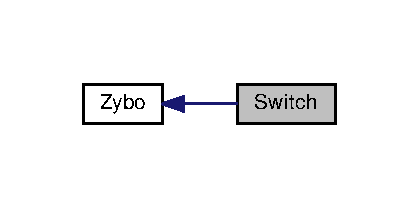
\includegraphics[width=201pt]{group___switch}
\end{center}
\end{figure}
\subsection*{Strutture dati}
\begin{DoxyCompactItemize}
\item 
struct \hyperlink{struct_zybo_switch__t}{Zybo\+Switch\+\_\+t}
\begin{DoxyCompactList}\small\item\em Struttura opaca che astrae l'insieme degli switch presenti sulla board Digilent Zybo;. \end{DoxyCompactList}\end{DoxyCompactItemize}
\subsection*{Definizioni}
\begin{DoxyCompactItemize}
\item 
\#define \hyperlink{group___switch_ga1c463f6e1e3a43f68109c176772ce5cc}{Zybo\+Switch}(i)~((uint32\+\_\+t)(1$<$$<$i))
\begin{DoxyCompactList}\small\item\em Metodo alternativo per la specifica di uno degli switch presenti sulla board Digilent Zybo. \end{DoxyCompactList}\end{DoxyCompactItemize}
\subsection*{Tipi enumerati (enum)}
\begin{DoxyCompactItemize}
\item 
enum \hyperlink{group___switch_ga2e0602a824354f25c395f938caba3703}{Zybo\+Switch\+\_\+mask\+\_\+t} \{ \hyperlink{group___switch_gga2e0602a824354f25c395f938caba3703a73ccea5ad8c919fe962e9a67a3733ee3}{Zybo\+Switch3} = 0x8, 
\hyperlink{group___switch_gga2e0602a824354f25c395f938caba3703aac2f5ebb28eb3bd93fcdf8019b6a3e9e}{Zybo\+Switch2} = 0x4, 
\hyperlink{group___switch_gga2e0602a824354f25c395f938caba3703a694a25c87b1ec597d2a6032bf5d34b0f}{Zybo\+Switch1} = 0x2, 
\hyperlink{group___switch_gga2e0602a824354f25c395f938caba3703a84350e8b6e7a7e2cabf22fc7a1a5c651}{Zybo\+Switch0} = 0x1
 \}
\begin{DoxyCompactList}\small\item\em Maschere di selezione degli switch. \end{DoxyCompactList}\item 
enum \hyperlink{group___switch_ga4ba6b49b2f47ebb464aefcea7e23e04a}{Zybo\+Switch\+\_\+status\+\_\+t} \{ \hyperlink{group___switch_gga4ba6b49b2f47ebb464aefcea7e23e04aa1d686faf83e8606e68eec0b7e525a755}{Zybo\+Switch\+\_\+off}, 
\hyperlink{group___switch_gga4ba6b49b2f47ebb464aefcea7e23e04aafba009508b8822de867af69034e3e4f8}{Zybo\+Switch\+\_\+on}
 \}
\begin{DoxyCompactList}\small\item\em Status di attivo/inattivo degli switch. \end{DoxyCompactList}\end{DoxyCompactItemize}
\subsection*{Funzioni}
\begin{DoxyCompactItemize}
\item 
void \hyperlink{group___switch_ga121018c0ccfeb05b6e8f692a5a6955d7}{Zybo\+Switch\+\_\+init} (\hyperlink{struct_zybo_switch__t}{Zybo\+Switch\+\_\+t} $\ast$switches, \hyperlink{struct_g_p_i_o__t}{G\+P\+I\+O\+\_\+t} $\ast$gpio, \hyperlink{group___g_p_i_o_ga6d5aef8a8a54ee2f602d47252ff66595}{G\+P\+I\+O\+\_\+mask} Switch3\+\_\+pin, \hyperlink{group___g_p_i_o_ga6d5aef8a8a54ee2f602d47252ff66595}{G\+P\+I\+O\+\_\+mask} Switch2\+\_\+pin, \hyperlink{group___g_p_i_o_ga6d5aef8a8a54ee2f602d47252ff66595}{G\+P\+I\+O\+\_\+mask} Switch1\+\_\+pin, \hyperlink{group___g_p_i_o_ga6d5aef8a8a54ee2f602d47252ff66595}{G\+P\+I\+O\+\_\+mask} Switch0\+\_\+pin)
\begin{DoxyCompactList}\small\item\em Inizializza un oggetto di tipo \hyperlink{struct_zybo_switch__t}{Zybo\+Switch\+\_\+t}. \end{DoxyCompactList}\item 
\hyperlink{group___switch_ga4ba6b49b2f47ebb464aefcea7e23e04a}{Zybo\+Switch\+\_\+status\+\_\+t} \hyperlink{group___switch_gafac8daf9a9a585f8f20ef2a6fa883a1f}{Zybo\+Switch\+\_\+get\+Status} (\hyperlink{struct_zybo_switch__t}{Zybo\+Switch\+\_\+t} $\ast$switches, \hyperlink{group___switch_ga2e0602a824354f25c395f938caba3703}{Zybo\+Switch\+\_\+mask\+\_\+t} mask)
\begin{DoxyCompactList}\small\item\em Permette la lettura dello stato degli switch presenti sulla board. \end{DoxyCompactList}\end{DoxyCompactItemize}


\subsection{Descrizione dettagliata}


\subsection{Documentazione delle definizioni}
\hypertarget{group___switch_ga1c463f6e1e3a43f68109c176772ce5cc}{\index{Switch@{Switch}!Zybo\+Switch@{Zybo\+Switch}}
\index{Zybo\+Switch@{Zybo\+Switch}!Switch@{Switch}}
\subsubsection[{Zybo\+Switch}]{\setlength{\rightskip}{0pt plus 5cm}\#define Zybo\+Switch(
\begin{DoxyParamCaption}
\item[{}]{i}
\end{DoxyParamCaption}
)~((uint32\+\_\+t)(1$<$$<$i))}}\label{group___switch_ga1c463f6e1e3a43f68109c176772ce5cc}


Metodo alternativo per la specifica di uno degli switch presenti sulla board Digilent Zybo. 


\begin{DoxyParams}{Parametri}
{\em i} & indice dello switch da selezionare, da 0 a 3 \\
\hline
\end{DoxyParams}
\begin{DoxyReturn}{Restituisce}
maschera di selezione dello switch i-\/esimo 
\end{DoxyReturn}


\subsection{Documentazione dei tipi enumerati}
\hypertarget{group___switch_ga2e0602a824354f25c395f938caba3703}{\index{Switch@{Switch}!Zybo\+Switch\+\_\+mask\+\_\+t@{Zybo\+Switch\+\_\+mask\+\_\+t}}
\index{Zybo\+Switch\+\_\+mask\+\_\+t@{Zybo\+Switch\+\_\+mask\+\_\+t}!Switch@{Switch}}
\subsubsection[{Zybo\+Switch\+\_\+mask\+\_\+t}]{\setlength{\rightskip}{0pt plus 5cm}enum {\bf Zybo\+Switch\+\_\+mask\+\_\+t}}}\label{group___switch_ga2e0602a824354f25c395f938caba3703}


Maschere di selezione degli switch. 

\begin{Desc}
\item[Valori del tipo enumerato]\par
\begin{description}
\index{Zybo\+Switch3@{Zybo\+Switch3}!Switch@{Switch}}\index{Switch@{Switch}!Zybo\+Switch3@{Zybo\+Switch3}}\item[{\em 
\hypertarget{group___switch_gga2e0602a824354f25c395f938caba3703a73ccea5ad8c919fe962e9a67a3733ee3}{Zybo\+Switch3}\label{group___switch_gga2e0602a824354f25c395f938caba3703a73ccea5ad8c919fe962e9a67a3733ee3}
}]Zybo\+Switch3, seleziona lo switch 3 sulla board Digilent Zybo;. \index{Zybo\+Switch2@{Zybo\+Switch2}!Switch@{Switch}}\index{Switch@{Switch}!Zybo\+Switch2@{Zybo\+Switch2}}\item[{\em 
\hypertarget{group___switch_gga2e0602a824354f25c395f938caba3703aac2f5ebb28eb3bd93fcdf8019b6a3e9e}{Zybo\+Switch2}\label{group___switch_gga2e0602a824354f25c395f938caba3703aac2f5ebb28eb3bd93fcdf8019b6a3e9e}
}]Zybo\+Switch2, seleziona lo switch 2 sulla board Digilent Zybo;. \index{Zybo\+Switch1@{Zybo\+Switch1}!Switch@{Switch}}\index{Switch@{Switch}!Zybo\+Switch1@{Zybo\+Switch1}}\item[{\em 
\hypertarget{group___switch_gga2e0602a824354f25c395f938caba3703a694a25c87b1ec597d2a6032bf5d34b0f}{Zybo\+Switch1}\label{group___switch_gga2e0602a824354f25c395f938caba3703a694a25c87b1ec597d2a6032bf5d34b0f}
}]Zybo\+Switch1, seleziona lo switch 1 sulla board Digilent Zybo;. \index{Zybo\+Switch0@{Zybo\+Switch0}!Switch@{Switch}}\index{Switch@{Switch}!Zybo\+Switch0@{Zybo\+Switch0}}\item[{\em 
\hypertarget{group___switch_gga2e0602a824354f25c395f938caba3703a84350e8b6e7a7e2cabf22fc7a1a5c651}{Zybo\+Switch0}\label{group___switch_gga2e0602a824354f25c395f938caba3703a84350e8b6e7a7e2cabf22fc7a1a5c651}
}]Zybo\+Switch0, seleziona lo switch 0 sulla board Digilent Zybo;. \end{description}
\end{Desc}
\hypertarget{group___switch_ga4ba6b49b2f47ebb464aefcea7e23e04a}{\index{Switch@{Switch}!Zybo\+Switch\+\_\+status\+\_\+t@{Zybo\+Switch\+\_\+status\+\_\+t}}
\index{Zybo\+Switch\+\_\+status\+\_\+t@{Zybo\+Switch\+\_\+status\+\_\+t}!Switch@{Switch}}
\subsubsection[{Zybo\+Switch\+\_\+status\+\_\+t}]{\setlength{\rightskip}{0pt plus 5cm}enum {\bf Zybo\+Switch\+\_\+status\+\_\+t}}}\label{group___switch_ga4ba6b49b2f47ebb464aefcea7e23e04a}


Status di attivo/inattivo degli switch. 

\begin{Desc}
\item[Valori del tipo enumerato]\par
\begin{description}
\index{Zybo\+Switch\+\_\+off@{Zybo\+Switch\+\_\+off}!Switch@{Switch}}\index{Switch@{Switch}!Zybo\+Switch\+\_\+off@{Zybo\+Switch\+\_\+off}}\item[{\em 
\hypertarget{group___switch_gga4ba6b49b2f47ebb464aefcea7e23e04aa1d686faf83e8606e68eec0b7e525a755}{Zybo\+Switch\+\_\+off}\label{group___switch_gga4ba6b49b2f47ebb464aefcea7e23e04aa1d686faf83e8606e68eec0b7e525a755}
}]Zybo\+Switch\+\_\+off, corrisponde al valore logico '0', indica che lo switch e' inattivo;. \index{Zybo\+Switch\+\_\+on@{Zybo\+Switch\+\_\+on}!Switch@{Switch}}\index{Switch@{Switch}!Zybo\+Switch\+\_\+on@{Zybo\+Switch\+\_\+on}}\item[{\em 
\hypertarget{group___switch_gga4ba6b49b2f47ebb464aefcea7e23e04aafba009508b8822de867af69034e3e4f8}{Zybo\+Switch\+\_\+on}\label{group___switch_gga4ba6b49b2f47ebb464aefcea7e23e04aafba009508b8822de867af69034e3e4f8}
}]Zybo\+Switch\+\_\+on, corrisponde al valore logico '1', indica che lo switch e' attivo;. \end{description}
\end{Desc}


\subsection{Documentazione delle funzioni}
\hypertarget{group___switch_gafac8daf9a9a585f8f20ef2a6fa883a1f}{\index{Switch@{Switch}!Zybo\+Switch\+\_\+get\+Status@{Zybo\+Switch\+\_\+get\+Status}}
\index{Zybo\+Switch\+\_\+get\+Status@{Zybo\+Switch\+\_\+get\+Status}!Switch@{Switch}}
\subsubsection[{Zybo\+Switch\+\_\+get\+Status}]{\setlength{\rightskip}{0pt plus 5cm}{\bf Zybo\+Switch\+\_\+status\+\_\+t} Zybo\+Switch\+\_\+get\+Status (
\begin{DoxyParamCaption}
\item[{{\bf Zybo\+Switch\+\_\+t} $\ast$}]{switches, }
\item[{{\bf Zybo\+Switch\+\_\+mask\+\_\+t}}]{mask}
\end{DoxyParamCaption}
)}}\label{group___switch_gafac8daf9a9a585f8f20ef2a6fa883a1f}


Permette la lettura dello stato degli switch presenti sulla board. 


\begin{DoxyParams}{Parametri}
{\em switches} & puntatore a struttura \hyperlink{struct_zybo_switch__t}{Zybo\+Switch\+\_\+t}, che astrae l'insieme degli switch presenti sulla board Digilent Zybo; \\
\hline
{\em mask} & maschera di selezione degli switch, quelli non selezionati non vengono tenuti in considerazione \\
\hline
\end{DoxyParams}
\begin{DoxyReturn}{Restituisce}
status status degli switch 
\end{DoxyReturn}

\begin{DoxyRetVals}{Valori di ritorno}
{\em Zybo\+Switch\+\_\+on} & se uno degli switch selezionati e' attivo; \\
\hline
{\em Zybo\+Switch\+\_\+off} & altrimenti\\
\hline
\end{DoxyRetVals}

\begin{DoxyCode}
1 ZyboSwitch\_status\_t switch\_status = ZyboSwitch\_getStatus(&switches, ZyboSwitch3);           // leggo lo
       stato dello switch 3
2 ZyboLed\_status\_t led\_status = (switch\_status == ZyboSwitch\_on ? ZyboLed\_on : ZyboLed\_off);  // se lo switch
       3 e' attivo accendo il led 3
3 ZyboLed\_setStatus(&leds, ZyboLed3, led\_status);                                             //
       accendo/spengo led 3
\end{DoxyCode}


\begin{DoxyWarning}{Avvertimento}
Usa la macro assert per verificare che\+:
\begin{DoxyItemize}
\item switches non sia un puntatore nullo;
\item switches-\/$>$gpio non sia un puntatore nullo 
\end{DoxyItemize}
\end{DoxyWarning}
\hypertarget{group___switch_ga121018c0ccfeb05b6e8f692a5a6955d7}{\index{Switch@{Switch}!Zybo\+Switch\+\_\+init@{Zybo\+Switch\+\_\+init}}
\index{Zybo\+Switch\+\_\+init@{Zybo\+Switch\+\_\+init}!Switch@{Switch}}
\subsubsection[{Zybo\+Switch\+\_\+init}]{\setlength{\rightskip}{0pt plus 5cm}void Zybo\+Switch\+\_\+init (
\begin{DoxyParamCaption}
\item[{{\bf Zybo\+Switch\+\_\+t} $\ast$}]{switches, }
\item[{{\bf G\+P\+I\+O\+\_\+t} $\ast$}]{gpio, }
\item[{{\bf G\+P\+I\+O\+\_\+mask}}]{Switch3\+\_\+pin, }
\item[{{\bf G\+P\+I\+O\+\_\+mask}}]{Switch2\+\_\+pin, }
\item[{{\bf G\+P\+I\+O\+\_\+mask}}]{Switch1\+\_\+pin, }
\item[{{\bf G\+P\+I\+O\+\_\+mask}}]{Switch0\+\_\+pin}
\end{DoxyParamCaption}
)}}\label{group___switch_ga121018c0ccfeb05b6e8f692a5a6955d7}


Inizializza un oggetto di tipo \hyperlink{struct_zybo_switch__t}{Zybo\+Switch\+\_\+t}. 


\begin{DoxyParams}{Parametri}
{\em switches} & puntatore a struttura \hyperlink{struct_zybo_switch__t}{Zybo\+Switch\+\_\+t}, che astrae l'insieme degli switch presenti sulla board Digilent Zybo; \\
\hline
{\em gpio} & puntatore a struttura \hyperlink{struct_g_p_i_o__t}{G\+P\+I\+O\+\_\+t}, che astrae un device G\+P\+I\+O; non viene inizializzato dalla funziona, sara' necessario inizializzarlo preventivamente; si faccia riferimento all'esempio riportato di seguito \\
\hline
{\em Switch3\+\_\+pin} & pin del device G\+P\+I\+O a cui e' associato lo switch 3 della board Digilent Zybo; \\
\hline
{\em Switch2\+\_\+pin} & pin del device G\+P\+I\+O a cui e' associato lo switch 2 della board Digilent Zybo; \\
\hline
{\em Switch1\+\_\+pin} & pin del device G\+P\+I\+O a cui e' associato lo switch 1 della board Digilent Zybo; \\
\hline
{\em Switch0\+\_\+pin} & pin del device G\+P\+I\+O a cui e' associato lo switch 0 della board Digilent Zybo;\\
\hline
\end{DoxyParams}

\begin{DoxyCode}
1 GPIO\_t gpioSwitch;
2 GPIO\_init(&gpioSwitch, XPAR\_MYGPIO\_1\_S00\_AXI\_BASEADDR, 4, 0, 4, 8);
3 ZyboSwitch\_t switches;
4 ZyboSwitch\_init(&switches, &gpioSwitch, GPIO\_pin3, GPIO\_pin2, GPIO\_pin1, GPIO\_pin0);
\end{DoxyCode}


\begin{DoxyWarning}{Avvertimento}
Usa la macro assert per verificare che\+:
\begin{DoxyItemize}
\item switches non sia un puntatore nullo;
\item gpio non sia un puntatore nullo
\item Switch\+N\+\_\+pin siano tutti pin differenti 
\end{DoxyItemize}
\end{DoxyWarning}

\hypertarget{group__my_g_p_i_o}{\section{My\+G\+P\+I\+O}
\label{group__my_g_p_i_o}\index{My\+G\+P\+I\+O@{My\+G\+P\+I\+O}}
}
Diagramma di collaborazione per My\+G\+P\+I\+O\+:\nopagebreak
\begin{figure}[H]
\begin{center}
\leavevmode
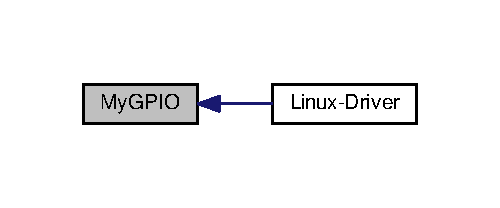
\includegraphics[width=240pt]{group__my_g_p_i_o}
\end{center}
\end{figure}
\subsection*{Moduli}
\begin{DoxyCompactItemize}
\item 
\hyperlink{group___linux-_driver}{Linux-\/\+Driver}
\end{DoxyCompactItemize}
\subsection*{Strutture dati}
\begin{DoxyCompactItemize}
\item 
struct \hyperlink{structmy_g_p_i_o__t}{my\+G\+P\+I\+O\+\_\+t}
\begin{DoxyCompactList}\small\item\em Struttura che astrae un device my\+G\+P\+I\+O. \end{DoxyCompactList}\end{DoxyCompactItemize}
\subsection*{Definizioni}
\begin{DoxyCompactItemize}
\item 
\#define \hyperlink{group__my_g_p_i_o_ga81a662103d6ed053978c0a9b4c273065}{my\+G\+P\+I\+O\+\_\+\+M\+O\+D\+E\+\_\+\+O\+F\+F\+S\+E\+T}~0\+U
\begin{DoxyCompactList}\small\item\em Offset, rispetto all'indirizzo base, del registro \char`\"{}mode\char`\"{} per il device my\+G\+P\+I\+O. \end{DoxyCompactList}\item 
\#define \hyperlink{group__my_g_p_i_o_ga2e45778b6ca9ce6f5768b3f7a4557ce1}{my\+G\+P\+I\+O\+\_\+\+W\+R\+I\+T\+E\+\_\+\+O\+F\+F\+S\+E\+T}~4\+U
\begin{DoxyCompactList}\small\item\em Offset, rispetto all'indirizzo base, del registro \char`\"{}write\char`\"{} per il device my\+G\+P\+I\+O. \end{DoxyCompactList}\item 
\#define \hyperlink{group__my_g_p_i_o_ga584d2dfece76e5762030d918d80592cc}{my\+G\+P\+I\+O\+\_\+\+R\+E\+A\+D\+\_\+\+O\+F\+F\+S\+E\+T}~8\+U
\begin{DoxyCompactList}\small\item\em Offset, rispetto all'indirizzo base, del registro \char`\"{}read\char`\"{} per il device my\+G\+P\+I\+O. \end{DoxyCompactList}\item 
\#define \hyperlink{group__my_g_p_i_o_gaacf2d8a21a051e778f02f8811b9c1e96}{my\+G\+P\+I\+O\+\_\+\+I\+N\+T\+R\+\_\+\+O\+F\+F\+S\+E\+T}~12\+U
\begin{DoxyCompactList}\small\item\em Offset, rispetto all'indirizzo base, del registro \char`\"{}interrupt\char`\"{} per il device my\+G\+P\+I\+O. \end{DoxyCompactList}\item 
\#define \hyperlink{group__my_g_p_i_o_ga0ba32e2adf874ed7216c5993369153e1}{my\+G\+P\+I\+O\+\_\+\+I\+N\+T\+R\+\_\+\+Int\+En\+\_\+mask}~0x1\+U
\begin{DoxyCompactList}\small\item\em maschera del bit del registro \char`\"{}interrupt\char`\"{} che funge da interrupt-\/enable, per il device my\+G\+P\+I\+O \end{DoxyCompactList}\item 
\#define \hyperlink{group__my_g_p_i_o_ga4cd02635783bc2a4ad7639cfb9fdb698}{my\+G\+P\+I\+O\+\_\+\+I\+N\+T\+R\+\_\+\+Irq\+\_\+mask}~0x2\+U
\begin{DoxyCompactList}\small\item\em maschera del bit del registro \char`\"{}interrupt\char`\"{} che funge da interrupt-\/request, per il device my\+G\+P\+I\+O \end{DoxyCompactList}\item 
\#define \hyperlink{group__my_g_p_i_o_gaa760b8397e6372e48c1008c2ba8d7387}{my\+G\+P\+I\+O\+\_\+\+I\+N\+T\+R\+\_\+\+Int\+Ack\+\_\+mask}~0x4\+U
\begin{DoxyCompactList}\small\item\em maschera del bit del registro \char`\"{}interrupt\char`\"{} che funge da interrupt-\/ack, per il device my\+G\+P\+I\+O \end{DoxyCompactList}\item 
\#define \hyperlink{group__my_g_p_i_o_gabbe2491a3b71c292521025b7b382b971}{my\+G\+P\+I\+O\+\_\+pin}(i)~((uint32\+\_\+t)(1$<$$<$(i)))
\begin{DoxyCompactList}\small\item\em Metodo alternativo per la specifica di uno dei pin di un device my\+G\+P\+I\+O. \end{DoxyCompactList}\end{DoxyCompactItemize}
\subsection*{Tipi enumerati (enum)}
\begin{DoxyCompactItemize}
\item 
enum \hyperlink{group__my_g_p_i_o_ga402a0d20afc0cb7c25554b8b023f4253}{my\+G\+P\+I\+O\+\_\+mask} \{ \\*
\hyperlink{group__my_g_p_i_o_gga402a0d20afc0cb7c25554b8b023f4253a6db6fa7be955ae379f543d96122e23a9}{my\+G\+P\+I\+O\+\_\+pin0} = 0x1\+U, 
\hyperlink{group__my_g_p_i_o_gga402a0d20afc0cb7c25554b8b023f4253a1de6bdcc01efca2c39f584f5a20293be}{my\+G\+P\+I\+O\+\_\+pin1} = 0x2\+U, 
\hyperlink{group__my_g_p_i_o_gga402a0d20afc0cb7c25554b8b023f4253a1fb3f52d920ac8ba17b74dd73c27d783}{my\+G\+P\+I\+O\+\_\+pin2} = 0x4\+U, 
\hyperlink{group__my_g_p_i_o_gga402a0d20afc0cb7c25554b8b023f4253a4514d64390392b626aa4dbfaac8dc1e5}{my\+G\+P\+I\+O\+\_\+pin3} = 0x8\+U, 
\\*
\hyperlink{group__my_g_p_i_o_gga402a0d20afc0cb7c25554b8b023f4253a0a446f53dee6f6f4ccb9a1d1f947b637}{my\+G\+P\+I\+O\+\_\+pin4} = 0x10\+U, 
\hyperlink{group__my_g_p_i_o_gga402a0d20afc0cb7c25554b8b023f4253a04a111036a27e9b97f0950f6d37b04d2}{my\+G\+P\+I\+O\+\_\+pin5} = 0x20\+U, 
\hyperlink{group__my_g_p_i_o_gga402a0d20afc0cb7c25554b8b023f4253a39a529f8c0a4f302029f54daa815471b}{my\+G\+P\+I\+O\+\_\+pin6} = 0x40\+U, 
\hyperlink{group__my_g_p_i_o_gga402a0d20afc0cb7c25554b8b023f4253af4e88b077442e4c0f459e1e4aa60626b}{my\+G\+P\+I\+O\+\_\+pin7} = 0x80\+U, 
\\*
\hyperlink{group__my_g_p_i_o_gga402a0d20afc0cb7c25554b8b023f4253a615159bcf4e347dc2b60f2545fae5f9e}{my\+G\+P\+I\+O\+\_\+pin8} = 0x100\+U, 
\hyperlink{group__my_g_p_i_o_gga402a0d20afc0cb7c25554b8b023f4253a8d721236fb936126a08c12b87696f6e9}{my\+G\+P\+I\+O\+\_\+pin9} = 0x200\+U, 
\hyperlink{group__my_g_p_i_o_gga402a0d20afc0cb7c25554b8b023f4253ae3067b7b3b1a2e171ecd74b6abd48341}{my\+G\+P\+I\+O\+\_\+pin10} = 0x400\+U, 
\hyperlink{group__my_g_p_i_o_gga402a0d20afc0cb7c25554b8b023f4253ae5c2e65508bfd452100d9da331d6220a}{my\+G\+P\+I\+O\+\_\+pin11} = 0x800\+U, 
\\*
\hyperlink{group__my_g_p_i_o_gga402a0d20afc0cb7c25554b8b023f4253afa75e3c1c019048c8553cb733c5137b5}{my\+G\+P\+I\+O\+\_\+pin12} = 0x1000\+U, 
\hyperlink{group__my_g_p_i_o_gga402a0d20afc0cb7c25554b8b023f4253a243381a796f0936a576f184dd115b37c}{my\+G\+P\+I\+O\+\_\+pin13} = 0x2000\+U, 
\hyperlink{group__my_g_p_i_o_gga402a0d20afc0cb7c25554b8b023f4253aed4915d6b3eab49cc1ba971b9f439fdd}{my\+G\+P\+I\+O\+\_\+pin14} = 0x4000\+U, 
\hyperlink{group__my_g_p_i_o_gga402a0d20afc0cb7c25554b8b023f4253a46c427ea97182a77e8c975d3429a64ee}{my\+G\+P\+I\+O\+\_\+pin15} = 0x8000\+U, 
\\*
\hyperlink{group__my_g_p_i_o_gga402a0d20afc0cb7c25554b8b023f4253a5a27c4d87207b2eba865876854f1ba67}{my\+G\+P\+I\+O\+\_\+pin16} = 0x10000\+U, 
\hyperlink{group__my_g_p_i_o_gga402a0d20afc0cb7c25554b8b023f4253ab0541af31059bdc8dca44d5dafa7e779}{my\+G\+P\+I\+O\+\_\+pin17} = 0x20000\+U, 
\hyperlink{group__my_g_p_i_o_gga402a0d20afc0cb7c25554b8b023f4253a7a51a492e3cb580581a2c8eb439edd99}{my\+G\+P\+I\+O\+\_\+pin18} = 0x40000\+U, 
\hyperlink{group__my_g_p_i_o_gga402a0d20afc0cb7c25554b8b023f4253a9118ae2775e93bd4522660e81a2d5309}{my\+G\+P\+I\+O\+\_\+pin19} = 0x80000\+U, 
\\*
\hyperlink{group__my_g_p_i_o_gga402a0d20afc0cb7c25554b8b023f4253a7940782a16f88dbbb3a4037c2bef1711}{my\+G\+P\+I\+O\+\_\+pin20} = 0x100000\+U, 
\hyperlink{group__my_g_p_i_o_gga402a0d20afc0cb7c25554b8b023f4253a1da616a8cf4396927db1e5a336fb6dc5}{my\+G\+P\+I\+O\+\_\+pin21} = 0x200000\+U, 
\hyperlink{group__my_g_p_i_o_gga402a0d20afc0cb7c25554b8b023f4253acf80113da8d789f7da9f9edc4ab6003c}{my\+G\+P\+I\+O\+\_\+pin22} = 0x400000\+U, 
\hyperlink{group__my_g_p_i_o_gga402a0d20afc0cb7c25554b8b023f4253ad64e03b703608de173ab5950b5121830}{my\+G\+P\+I\+O\+\_\+pin23} = 0x800000\+U, 
\\*
\hyperlink{group__my_g_p_i_o_gga402a0d20afc0cb7c25554b8b023f4253a5bb93f546327123f81b06ed0dfcdf110}{my\+G\+P\+I\+O\+\_\+pin24} = 0x1000000\+U, 
\hyperlink{group__my_g_p_i_o_gga402a0d20afc0cb7c25554b8b023f4253a0b27a7e78aff5836f33085f3b4539f56}{my\+G\+P\+I\+O\+\_\+pin25} = 0x2000000\+U, 
\hyperlink{group__my_g_p_i_o_gga402a0d20afc0cb7c25554b8b023f4253aaa07c24140250dcbc695206793efa8af}{my\+G\+P\+I\+O\+\_\+pin26} = 0x4000000\+U, 
\hyperlink{group__my_g_p_i_o_gga402a0d20afc0cb7c25554b8b023f4253a1dd5e99eba6237aeb30b2194c553c37f}{my\+G\+P\+I\+O\+\_\+pin27} = 0x8000000\+U, 
\\*
\hyperlink{group__my_g_p_i_o_gga402a0d20afc0cb7c25554b8b023f4253a2076590efec8bcf9ef3285798753e632}{my\+G\+P\+I\+O\+\_\+pin28} = 0x10000000\+U, 
\hyperlink{group__my_g_p_i_o_gga402a0d20afc0cb7c25554b8b023f4253abfe9540fa3946a35e20f7f68cb1b8084}{my\+G\+P\+I\+O\+\_\+pin29} = 0x20000000\+U, 
\hyperlink{group__my_g_p_i_o_gga402a0d20afc0cb7c25554b8b023f4253a59993a30c537c116eddb42d10778f4f8}{my\+G\+P\+I\+O\+\_\+pin30} = 0x40000000\+U, 
\hyperlink{group__my_g_p_i_o_gga402a0d20afc0cb7c25554b8b023f4253a9a55b7c245bd9aad750b7891d27e9225}{my\+G\+P\+I\+O\+\_\+pin31} = 0x80000000\+U, 
\\*
\hyperlink{group__my_g_p_i_o_gga402a0d20afc0cb7c25554b8b023f4253a0347b1742eef6b2575a7d409c7fb5c3d}{my\+G\+P\+I\+O\+\_\+byte0} = 0x000000ff\+U, 
\hyperlink{group__my_g_p_i_o_gga402a0d20afc0cb7c25554b8b023f4253ae5aec65fa20f554b893e419fc2755fd0}{my\+G\+P\+I\+O\+\_\+byte1} = 0x0000ff00\+U, 
\hyperlink{group__my_g_p_i_o_gga402a0d20afc0cb7c25554b8b023f4253af4892f7db28c64a7cf2a7236c88b742b}{my\+G\+P\+I\+O\+\_\+byte2} = 0x00ff0000\+U, 
\hyperlink{group__my_g_p_i_o_gga402a0d20afc0cb7c25554b8b023f4253a1ceefb9d65397352e986c573984d0129}{my\+G\+P\+I\+O\+\_\+byte3} = 0xff000000\+U
 \}
\begin{DoxyCompactList}\small\item\em Maschere di selezione dei pin di un device my\+G\+P\+I\+O. \end{DoxyCompactList}\item 
enum \hyperlink{group__my_g_p_i_o_ga76b849f0e0c05e7f9161bdb33396f2b1}{my\+G\+P\+I\+O\+\_\+mode} \{ \hyperlink{group__my_g_p_i_o_gga76b849f0e0c05e7f9161bdb33396f2b1a1e6dc78e7641e878cadc842d39605d5d}{my\+G\+P\+I\+O\+\_\+read}, 
\hyperlink{group__my_g_p_i_o_gga76b849f0e0c05e7f9161bdb33396f2b1a2d66976280eb7595a42c631683bdfad6}{my\+G\+P\+I\+O\+\_\+write}
 \}
\begin{DoxyCompactList}\small\item\em my\+G\+P\+I\+O\+\_\+mode, modalita' di funzionamento (lettura/scrittura) di un device my\+G\+P\+I\+O \end{DoxyCompactList}\item 
enum \hyperlink{group__my_g_p_i_o_gaf634fe4a0e1eab8da5000b72d6ad362b}{my\+G\+P\+I\+O\+\_\+value} \{ \hyperlink{group__my_g_p_i_o_ggaf634fe4a0e1eab8da5000b72d6ad362ba98cde80dbda025bd1ae7231c76b55674}{my\+G\+P\+I\+O\+\_\+reset}, 
\hyperlink{group__my_g_p_i_o_ggaf634fe4a0e1eab8da5000b72d6ad362ba10d296f3711d01189cc6c2d87f7c9149}{my\+G\+P\+I\+O\+\_\+set}
 \}
\begin{DoxyCompactList}\small\item\em my\+G\+P\+I\+O\+\_\+value, valore di un my\+G\+P\+I\+O \end{DoxyCompactList}\end{DoxyCompactItemize}
\subsection*{Funzioni}
\begin{DoxyCompactItemize}
\item 
void \hyperlink{group__my_g_p_i_o_ga8fda7ca73b187baf256409423c25d725}{my\+G\+P\+I\+O\+\_\+init} (\hyperlink{structmy_g_p_i_o__t}{my\+G\+P\+I\+O\+\_\+t} $\ast$gpio, uint32\+\_\+t base\+\_\+address)
\begin{DoxyCompactList}\small\item\em Inizializza un device my\+G\+P\+I\+O. \end{DoxyCompactList}\item 
void \hyperlink{group__my_g_p_i_o_ga38a2ea04d07af50f7f570f0367594c8b}{my\+G\+P\+I\+O\+\_\+set\+Mode} (\hyperlink{structmy_g_p_i_o__t}{my\+G\+P\+I\+O\+\_\+t} $\ast$gpio, \hyperlink{group__my_g_p_i_o_ga402a0d20afc0cb7c25554b8b023f4253}{my\+G\+P\+I\+O\+\_\+mask} mask, \hyperlink{group__my_g_p_i_o_ga76b849f0e0c05e7f9161bdb33396f2b1}{my\+G\+P\+I\+O\+\_\+mode} mode)
\begin{DoxyCompactList}\small\item\em Permette di settare la modalita' lettura/scrittura dei pin di un device my\+G\+P\+I\+O;. \end{DoxyCompactList}\item 
void \hyperlink{group__my_g_p_i_o_gab742e68093ad4c90fe299b64fd6736ca}{my\+G\+P\+I\+O\+\_\+set\+Value} (\hyperlink{structmy_g_p_i_o__t}{my\+G\+P\+I\+O\+\_\+t} $\ast$gpio, \hyperlink{group__my_g_p_i_o_ga402a0d20afc0cb7c25554b8b023f4253}{my\+G\+P\+I\+O\+\_\+mask} mask, \hyperlink{group__my_g_p_i_o_gaf634fe4a0e1eab8da5000b72d6ad362b}{my\+G\+P\+I\+O\+\_\+value} value)
\begin{DoxyCompactList}\small\item\em Permette di settare il valore dei pin di un device my\+G\+P\+I\+O, se configurati come output. \end{DoxyCompactList}\item 
void \hyperlink{group__my_g_p_i_o_ga27ea411bf51a58fe48eb8c5036780b53}{my\+G\+P\+I\+O\+\_\+toggle} (\hyperlink{structmy_g_p_i_o__t}{my\+G\+P\+I\+O\+\_\+t} $\ast$gpio, \hyperlink{group__my_g_p_i_o_ga402a0d20afc0cb7c25554b8b023f4253}{my\+G\+P\+I\+O\+\_\+mask} mask)
\begin{DoxyCompactList}\small\item\em Permette di invertire il valore dei pin di un device my\+G\+P\+I\+O, se configurati come output. \end{DoxyCompactList}\item 
\hyperlink{group__my_g_p_i_o_gaf634fe4a0e1eab8da5000b72d6ad362b}{my\+G\+P\+I\+O\+\_\+value} \hyperlink{group__my_g_p_i_o_gad6576f1d0fb17d9b492da0b1008550d0}{my\+G\+P\+I\+O\+\_\+get\+Value} (\hyperlink{structmy_g_p_i_o__t}{my\+G\+P\+I\+O\+\_\+t} $\ast$gpio, \hyperlink{group__my_g_p_i_o_ga402a0d20afc0cb7c25554b8b023f4253}{my\+G\+P\+I\+O\+\_\+mask} mask)
\begin{DoxyCompactList}\small\item\em Permette di leggere il valore dei pin di un device my\+G\+P\+I\+O;. \end{DoxyCompactList}\item 
\hyperlink{group__my_g_p_i_o_ga402a0d20afc0cb7c25554b8b023f4253}{my\+G\+P\+I\+O\+\_\+mask} \hyperlink{group__my_g_p_i_o_gadb3ecd03ea82420488977134c9313e18}{my\+G\+P\+I\+O\+\_\+get\+Read} (\hyperlink{structmy_g_p_i_o__t}{my\+G\+P\+I\+O\+\_\+t} $\ast$gpio)
\begin{DoxyCompactList}\small\item\em Restituisce la maschera dei pin settati di un device my\+G\+P\+I\+O. \end{DoxyCompactList}\item 
void \hyperlink{group__my_g_p_i_o_ga39822bfa495a9388e81ced74884c06a2}{my\+G\+P\+I\+O\+\_\+interrupt\+Enable} (\hyperlink{structmy_g_p_i_o__t}{my\+G\+P\+I\+O\+\_\+t} $\ast$gpio)
\begin{DoxyCompactList}\small\item\em Abilita gli interrupt per un device my\+G\+P\+I\+O. \end{DoxyCompactList}\item 
void \hyperlink{group__my_g_p_i_o_gab681db0119860bfad2c3e674289d8b3d}{my\+G\+P\+I\+O\+\_\+interrupt\+Disable} (\hyperlink{structmy_g_p_i_o__t}{my\+G\+P\+I\+O\+\_\+t} $\ast$gpio)
\begin{DoxyCompactList}\small\item\em Disabilita gli interrupt per un device my\+G\+P\+I\+O. \end{DoxyCompactList}\item 
void \hyperlink{group__my_g_p_i_o_ga396f6e5e7f0eeff01e98fcc78523402b}{my\+G\+P\+I\+O\+\_\+interrupt\+Ack} (\hyperlink{structmy_g_p_i_o__t}{my\+G\+P\+I\+O\+\_\+t} $\ast$gpio)
\begin{DoxyCompactList}\small\item\em Segnala al device che l'interruzione da lui sollevata e' stata servita. \end{DoxyCompactList}\item 
\hyperlink{group__my_g_p_i_o_gaf634fe4a0e1eab8da5000b72d6ad362b}{my\+G\+P\+I\+O\+\_\+value} \hyperlink{group__my_g_p_i_o_ga7936b506b45f116de68ddf06c84cc242}{my\+G\+P\+I\+O\+\_\+get\+Irq} (\hyperlink{structmy_g_p_i_o__t}{my\+G\+P\+I\+O\+\_\+t} $\ast$gpio)
\begin{DoxyCompactList}\small\item\em Consente di verificare se un device my\+G\+P\+I\+O abbia generato un'interruzione. \end{DoxyCompactList}\end{DoxyCompactItemize}


\subsection{Descrizione dettagliata}
Il modulo definisce un driver O\+O-\/like per l'utilizzo di una periferica my\+G\+P\+I\+O custom. 

\subsection{Documentazione delle definizioni}
\hypertarget{group__my_g_p_i_o_gaa760b8397e6372e48c1008c2ba8d7387}{\index{My\+G\+P\+I\+O@{My\+G\+P\+I\+O}!my\+G\+P\+I\+O\+\_\+\+I\+N\+T\+R\+\_\+\+Int\+Ack\+\_\+mask@{my\+G\+P\+I\+O\+\_\+\+I\+N\+T\+R\+\_\+\+Int\+Ack\+\_\+mask}}
\index{my\+G\+P\+I\+O\+\_\+\+I\+N\+T\+R\+\_\+\+Int\+Ack\+\_\+mask@{my\+G\+P\+I\+O\+\_\+\+I\+N\+T\+R\+\_\+\+Int\+Ack\+\_\+mask}!My\+G\+P\+I\+O@{My\+G\+P\+I\+O}}
\subsubsection[{my\+G\+P\+I\+O\+\_\+\+I\+N\+T\+R\+\_\+\+Int\+Ack\+\_\+mask}]{\setlength{\rightskip}{0pt plus 5cm}\#define my\+G\+P\+I\+O\+\_\+\+I\+N\+T\+R\+\_\+\+Int\+Ack\+\_\+mask~0x4\+U}}\label{group__my_g_p_i_o_gaa760b8397e6372e48c1008c2ba8d7387}


maschera del bit del registro \char`\"{}interrupt\char`\"{} che funge da interrupt-\/ack, per il device my\+G\+P\+I\+O 

\hypertarget{group__my_g_p_i_o_ga0ba32e2adf874ed7216c5993369153e1}{\index{My\+G\+P\+I\+O@{My\+G\+P\+I\+O}!my\+G\+P\+I\+O\+\_\+\+I\+N\+T\+R\+\_\+\+Int\+En\+\_\+mask@{my\+G\+P\+I\+O\+\_\+\+I\+N\+T\+R\+\_\+\+Int\+En\+\_\+mask}}
\index{my\+G\+P\+I\+O\+\_\+\+I\+N\+T\+R\+\_\+\+Int\+En\+\_\+mask@{my\+G\+P\+I\+O\+\_\+\+I\+N\+T\+R\+\_\+\+Int\+En\+\_\+mask}!My\+G\+P\+I\+O@{My\+G\+P\+I\+O}}
\subsubsection[{my\+G\+P\+I\+O\+\_\+\+I\+N\+T\+R\+\_\+\+Int\+En\+\_\+mask}]{\setlength{\rightskip}{0pt plus 5cm}\#define my\+G\+P\+I\+O\+\_\+\+I\+N\+T\+R\+\_\+\+Int\+En\+\_\+mask~0x1\+U}}\label{group__my_g_p_i_o_ga0ba32e2adf874ed7216c5993369153e1}


maschera del bit del registro \char`\"{}interrupt\char`\"{} che funge da interrupt-\/enable, per il device my\+G\+P\+I\+O 

\hypertarget{group__my_g_p_i_o_ga4cd02635783bc2a4ad7639cfb9fdb698}{\index{My\+G\+P\+I\+O@{My\+G\+P\+I\+O}!my\+G\+P\+I\+O\+\_\+\+I\+N\+T\+R\+\_\+\+Irq\+\_\+mask@{my\+G\+P\+I\+O\+\_\+\+I\+N\+T\+R\+\_\+\+Irq\+\_\+mask}}
\index{my\+G\+P\+I\+O\+\_\+\+I\+N\+T\+R\+\_\+\+Irq\+\_\+mask@{my\+G\+P\+I\+O\+\_\+\+I\+N\+T\+R\+\_\+\+Irq\+\_\+mask}!My\+G\+P\+I\+O@{My\+G\+P\+I\+O}}
\subsubsection[{my\+G\+P\+I\+O\+\_\+\+I\+N\+T\+R\+\_\+\+Irq\+\_\+mask}]{\setlength{\rightskip}{0pt plus 5cm}\#define my\+G\+P\+I\+O\+\_\+\+I\+N\+T\+R\+\_\+\+Irq\+\_\+mask~0x2\+U}}\label{group__my_g_p_i_o_ga4cd02635783bc2a4ad7639cfb9fdb698}


maschera del bit del registro \char`\"{}interrupt\char`\"{} che funge da interrupt-\/request, per il device my\+G\+P\+I\+O 

\hypertarget{group__my_g_p_i_o_gaacf2d8a21a051e778f02f8811b9c1e96}{\index{My\+G\+P\+I\+O@{My\+G\+P\+I\+O}!my\+G\+P\+I\+O\+\_\+\+I\+N\+T\+R\+\_\+\+O\+F\+F\+S\+E\+T@{my\+G\+P\+I\+O\+\_\+\+I\+N\+T\+R\+\_\+\+O\+F\+F\+S\+E\+T}}
\index{my\+G\+P\+I\+O\+\_\+\+I\+N\+T\+R\+\_\+\+O\+F\+F\+S\+E\+T@{my\+G\+P\+I\+O\+\_\+\+I\+N\+T\+R\+\_\+\+O\+F\+F\+S\+E\+T}!My\+G\+P\+I\+O@{My\+G\+P\+I\+O}}
\subsubsection[{my\+G\+P\+I\+O\+\_\+\+I\+N\+T\+R\+\_\+\+O\+F\+F\+S\+E\+T}]{\setlength{\rightskip}{0pt plus 5cm}\#define my\+G\+P\+I\+O\+\_\+\+I\+N\+T\+R\+\_\+\+O\+F\+F\+S\+E\+T~12\+U}}\label{group__my_g_p_i_o_gaacf2d8a21a051e778f02f8811b9c1e96}


Offset, rispetto all'indirizzo base, del registro \char`\"{}interrupt\char`\"{} per il device my\+G\+P\+I\+O. 

\hypertarget{group__my_g_p_i_o_ga81a662103d6ed053978c0a9b4c273065}{\index{My\+G\+P\+I\+O@{My\+G\+P\+I\+O}!my\+G\+P\+I\+O\+\_\+\+M\+O\+D\+E\+\_\+\+O\+F\+F\+S\+E\+T@{my\+G\+P\+I\+O\+\_\+\+M\+O\+D\+E\+\_\+\+O\+F\+F\+S\+E\+T}}
\index{my\+G\+P\+I\+O\+\_\+\+M\+O\+D\+E\+\_\+\+O\+F\+F\+S\+E\+T@{my\+G\+P\+I\+O\+\_\+\+M\+O\+D\+E\+\_\+\+O\+F\+F\+S\+E\+T}!My\+G\+P\+I\+O@{My\+G\+P\+I\+O}}
\subsubsection[{my\+G\+P\+I\+O\+\_\+\+M\+O\+D\+E\+\_\+\+O\+F\+F\+S\+E\+T}]{\setlength{\rightskip}{0pt plus 5cm}\#define my\+G\+P\+I\+O\+\_\+\+M\+O\+D\+E\+\_\+\+O\+F\+F\+S\+E\+T~0\+U}}\label{group__my_g_p_i_o_ga81a662103d6ed053978c0a9b4c273065}


Offset, rispetto all'indirizzo base, del registro \char`\"{}mode\char`\"{} per il device my\+G\+P\+I\+O. 

\hypertarget{group__my_g_p_i_o_gabbe2491a3b71c292521025b7b382b971}{\index{My\+G\+P\+I\+O@{My\+G\+P\+I\+O}!my\+G\+P\+I\+O\+\_\+pin@{my\+G\+P\+I\+O\+\_\+pin}}
\index{my\+G\+P\+I\+O\+\_\+pin@{my\+G\+P\+I\+O\+\_\+pin}!My\+G\+P\+I\+O@{My\+G\+P\+I\+O}}
\subsubsection[{my\+G\+P\+I\+O\+\_\+pin}]{\setlength{\rightskip}{0pt plus 5cm}\#define my\+G\+P\+I\+O\+\_\+pin(
\begin{DoxyParamCaption}
\item[{}]{i}
\end{DoxyParamCaption}
)~((uint32\+\_\+t)(1$<$$<$(i)))}}\label{group__my_g_p_i_o_gabbe2491a3b71c292521025b7b382b971}


Metodo alternativo per la specifica di uno dei pin di un device my\+G\+P\+I\+O. 


\begin{DoxyParams}[1]{Parametri}
\mbox{\tt in}  & {\em i} & indice del bit da selezionare, da 0 (bit meno significativo) a 31 (bit piu' significativo) \\
\hline
\end{DoxyParams}
\begin{DoxyReturn}{Restituisce}
maschera di selezione del pin i-\/esimo 
\end{DoxyReturn}
\hypertarget{group__my_g_p_i_o_ga584d2dfece76e5762030d918d80592cc}{\index{My\+G\+P\+I\+O@{My\+G\+P\+I\+O}!my\+G\+P\+I\+O\+\_\+\+R\+E\+A\+D\+\_\+\+O\+F\+F\+S\+E\+T@{my\+G\+P\+I\+O\+\_\+\+R\+E\+A\+D\+\_\+\+O\+F\+F\+S\+E\+T}}
\index{my\+G\+P\+I\+O\+\_\+\+R\+E\+A\+D\+\_\+\+O\+F\+F\+S\+E\+T@{my\+G\+P\+I\+O\+\_\+\+R\+E\+A\+D\+\_\+\+O\+F\+F\+S\+E\+T}!My\+G\+P\+I\+O@{My\+G\+P\+I\+O}}
\subsubsection[{my\+G\+P\+I\+O\+\_\+\+R\+E\+A\+D\+\_\+\+O\+F\+F\+S\+E\+T}]{\setlength{\rightskip}{0pt plus 5cm}\#define my\+G\+P\+I\+O\+\_\+\+R\+E\+A\+D\+\_\+\+O\+F\+F\+S\+E\+T~8\+U}}\label{group__my_g_p_i_o_ga584d2dfece76e5762030d918d80592cc}


Offset, rispetto all'indirizzo base, del registro \char`\"{}read\char`\"{} per il device my\+G\+P\+I\+O. 

\hypertarget{group__my_g_p_i_o_ga2e45778b6ca9ce6f5768b3f7a4557ce1}{\index{My\+G\+P\+I\+O@{My\+G\+P\+I\+O}!my\+G\+P\+I\+O\+\_\+\+W\+R\+I\+T\+E\+\_\+\+O\+F\+F\+S\+E\+T@{my\+G\+P\+I\+O\+\_\+\+W\+R\+I\+T\+E\+\_\+\+O\+F\+F\+S\+E\+T}}
\index{my\+G\+P\+I\+O\+\_\+\+W\+R\+I\+T\+E\+\_\+\+O\+F\+F\+S\+E\+T@{my\+G\+P\+I\+O\+\_\+\+W\+R\+I\+T\+E\+\_\+\+O\+F\+F\+S\+E\+T}!My\+G\+P\+I\+O@{My\+G\+P\+I\+O}}
\subsubsection[{my\+G\+P\+I\+O\+\_\+\+W\+R\+I\+T\+E\+\_\+\+O\+F\+F\+S\+E\+T}]{\setlength{\rightskip}{0pt plus 5cm}\#define my\+G\+P\+I\+O\+\_\+\+W\+R\+I\+T\+E\+\_\+\+O\+F\+F\+S\+E\+T~4\+U}}\label{group__my_g_p_i_o_ga2e45778b6ca9ce6f5768b3f7a4557ce1}


Offset, rispetto all'indirizzo base, del registro \char`\"{}write\char`\"{} per il device my\+G\+P\+I\+O. 



\subsection{Documentazione dei tipi enumerati}
\hypertarget{group__my_g_p_i_o_ga402a0d20afc0cb7c25554b8b023f4253}{\index{My\+G\+P\+I\+O@{My\+G\+P\+I\+O}!my\+G\+P\+I\+O\+\_\+mask@{my\+G\+P\+I\+O\+\_\+mask}}
\index{my\+G\+P\+I\+O\+\_\+mask@{my\+G\+P\+I\+O\+\_\+mask}!My\+G\+P\+I\+O@{My\+G\+P\+I\+O}}
\subsubsection[{my\+G\+P\+I\+O\+\_\+mask}]{\setlength{\rightskip}{0pt plus 5cm}enum {\bf my\+G\+P\+I\+O\+\_\+mask}}}\label{group__my_g_p_i_o_ga402a0d20afc0cb7c25554b8b023f4253}


Maschere di selezione dei pin di un device my\+G\+P\+I\+O. 

\begin{Desc}
\item[Valori del tipo enumerato]\par
\begin{description}
\index{my\+G\+P\+I\+O\+\_\+pin0@{my\+G\+P\+I\+O\+\_\+pin0}!My\+G\+P\+I\+O@{My\+G\+P\+I\+O}}\index{My\+G\+P\+I\+O@{My\+G\+P\+I\+O}!my\+G\+P\+I\+O\+\_\+pin0@{my\+G\+P\+I\+O\+\_\+pin0}}\item[{\em 
\hypertarget{group__my_g_p_i_o_gga402a0d20afc0cb7c25554b8b023f4253a6db6fa7be955ae379f543d96122e23a9}{my\+G\+P\+I\+O\+\_\+pin0}\label{group__my_g_p_i_o_gga402a0d20afc0cb7c25554b8b023f4253a6db6fa7be955ae379f543d96122e23a9}
}]my\+G\+P\+I\+O pin0 maschera di selezione del pin 0 di un device my\+G\+P\+I\+O \index{my\+G\+P\+I\+O\+\_\+pin1@{my\+G\+P\+I\+O\+\_\+pin1}!My\+G\+P\+I\+O@{My\+G\+P\+I\+O}}\index{My\+G\+P\+I\+O@{My\+G\+P\+I\+O}!my\+G\+P\+I\+O\+\_\+pin1@{my\+G\+P\+I\+O\+\_\+pin1}}\item[{\em 
\hypertarget{group__my_g_p_i_o_gga402a0d20afc0cb7c25554b8b023f4253a1de6bdcc01efca2c39f584f5a20293be}{my\+G\+P\+I\+O\+\_\+pin1}\label{group__my_g_p_i_o_gga402a0d20afc0cb7c25554b8b023f4253a1de6bdcc01efca2c39f584f5a20293be}
}]my\+G\+P\+I\+O pin1 maschera di selezione del pin 1 di un device my\+G\+P\+I\+O \index{my\+G\+P\+I\+O\+\_\+pin2@{my\+G\+P\+I\+O\+\_\+pin2}!My\+G\+P\+I\+O@{My\+G\+P\+I\+O}}\index{My\+G\+P\+I\+O@{My\+G\+P\+I\+O}!my\+G\+P\+I\+O\+\_\+pin2@{my\+G\+P\+I\+O\+\_\+pin2}}\item[{\em 
\hypertarget{group__my_g_p_i_o_gga402a0d20afc0cb7c25554b8b023f4253a1fb3f52d920ac8ba17b74dd73c27d783}{my\+G\+P\+I\+O\+\_\+pin2}\label{group__my_g_p_i_o_gga402a0d20afc0cb7c25554b8b023f4253a1fb3f52d920ac8ba17b74dd73c27d783}
}]my\+G\+P\+I\+O pin2 maschera di selezione del pin 2 di un device my\+G\+P\+I\+O \index{my\+G\+P\+I\+O\+\_\+pin3@{my\+G\+P\+I\+O\+\_\+pin3}!My\+G\+P\+I\+O@{My\+G\+P\+I\+O}}\index{My\+G\+P\+I\+O@{My\+G\+P\+I\+O}!my\+G\+P\+I\+O\+\_\+pin3@{my\+G\+P\+I\+O\+\_\+pin3}}\item[{\em 
\hypertarget{group__my_g_p_i_o_gga402a0d20afc0cb7c25554b8b023f4253a4514d64390392b626aa4dbfaac8dc1e5}{my\+G\+P\+I\+O\+\_\+pin3}\label{group__my_g_p_i_o_gga402a0d20afc0cb7c25554b8b023f4253a4514d64390392b626aa4dbfaac8dc1e5}
}]my\+G\+P\+I\+O pin3 maschera di selezione del pin 3 di un device my\+G\+P\+I\+O \index{my\+G\+P\+I\+O\+\_\+pin4@{my\+G\+P\+I\+O\+\_\+pin4}!My\+G\+P\+I\+O@{My\+G\+P\+I\+O}}\index{My\+G\+P\+I\+O@{My\+G\+P\+I\+O}!my\+G\+P\+I\+O\+\_\+pin4@{my\+G\+P\+I\+O\+\_\+pin4}}\item[{\em 
\hypertarget{group__my_g_p_i_o_gga402a0d20afc0cb7c25554b8b023f4253a0a446f53dee6f6f4ccb9a1d1f947b637}{my\+G\+P\+I\+O\+\_\+pin4}\label{group__my_g_p_i_o_gga402a0d20afc0cb7c25554b8b023f4253a0a446f53dee6f6f4ccb9a1d1f947b637}
}]my\+G\+P\+I\+O pin4 maschera di selezione del pin 4 di un device my\+G\+P\+I\+O \index{my\+G\+P\+I\+O\+\_\+pin5@{my\+G\+P\+I\+O\+\_\+pin5}!My\+G\+P\+I\+O@{My\+G\+P\+I\+O}}\index{My\+G\+P\+I\+O@{My\+G\+P\+I\+O}!my\+G\+P\+I\+O\+\_\+pin5@{my\+G\+P\+I\+O\+\_\+pin5}}\item[{\em 
\hypertarget{group__my_g_p_i_o_gga402a0d20afc0cb7c25554b8b023f4253a04a111036a27e9b97f0950f6d37b04d2}{my\+G\+P\+I\+O\+\_\+pin5}\label{group__my_g_p_i_o_gga402a0d20afc0cb7c25554b8b023f4253a04a111036a27e9b97f0950f6d37b04d2}
}]my\+G\+P\+I\+O pin5 maschera di selezione del pin 5 di un device my\+G\+P\+I\+O \index{my\+G\+P\+I\+O\+\_\+pin6@{my\+G\+P\+I\+O\+\_\+pin6}!My\+G\+P\+I\+O@{My\+G\+P\+I\+O}}\index{My\+G\+P\+I\+O@{My\+G\+P\+I\+O}!my\+G\+P\+I\+O\+\_\+pin6@{my\+G\+P\+I\+O\+\_\+pin6}}\item[{\em 
\hypertarget{group__my_g_p_i_o_gga402a0d20afc0cb7c25554b8b023f4253a39a529f8c0a4f302029f54daa815471b}{my\+G\+P\+I\+O\+\_\+pin6}\label{group__my_g_p_i_o_gga402a0d20afc0cb7c25554b8b023f4253a39a529f8c0a4f302029f54daa815471b}
}]my\+G\+P\+I\+O pin6 maschera di selezione del pin 6 di un device my\+G\+P\+I\+O \index{my\+G\+P\+I\+O\+\_\+pin7@{my\+G\+P\+I\+O\+\_\+pin7}!My\+G\+P\+I\+O@{My\+G\+P\+I\+O}}\index{My\+G\+P\+I\+O@{My\+G\+P\+I\+O}!my\+G\+P\+I\+O\+\_\+pin7@{my\+G\+P\+I\+O\+\_\+pin7}}\item[{\em 
\hypertarget{group__my_g_p_i_o_gga402a0d20afc0cb7c25554b8b023f4253af4e88b077442e4c0f459e1e4aa60626b}{my\+G\+P\+I\+O\+\_\+pin7}\label{group__my_g_p_i_o_gga402a0d20afc0cb7c25554b8b023f4253af4e88b077442e4c0f459e1e4aa60626b}
}]my\+G\+P\+I\+O pin7 maschera di selezione del pin 7 di un device my\+G\+P\+I\+O \index{my\+G\+P\+I\+O\+\_\+pin8@{my\+G\+P\+I\+O\+\_\+pin8}!My\+G\+P\+I\+O@{My\+G\+P\+I\+O}}\index{My\+G\+P\+I\+O@{My\+G\+P\+I\+O}!my\+G\+P\+I\+O\+\_\+pin8@{my\+G\+P\+I\+O\+\_\+pin8}}\item[{\em 
\hypertarget{group__my_g_p_i_o_gga402a0d20afc0cb7c25554b8b023f4253a615159bcf4e347dc2b60f2545fae5f9e}{my\+G\+P\+I\+O\+\_\+pin8}\label{group__my_g_p_i_o_gga402a0d20afc0cb7c25554b8b023f4253a615159bcf4e347dc2b60f2545fae5f9e}
}]my\+G\+P\+I\+O pin8 maschera di selezione del pin 8 di un device my\+G\+P\+I\+O \index{my\+G\+P\+I\+O\+\_\+pin9@{my\+G\+P\+I\+O\+\_\+pin9}!My\+G\+P\+I\+O@{My\+G\+P\+I\+O}}\index{My\+G\+P\+I\+O@{My\+G\+P\+I\+O}!my\+G\+P\+I\+O\+\_\+pin9@{my\+G\+P\+I\+O\+\_\+pin9}}\item[{\em 
\hypertarget{group__my_g_p_i_o_gga402a0d20afc0cb7c25554b8b023f4253a8d721236fb936126a08c12b87696f6e9}{my\+G\+P\+I\+O\+\_\+pin9}\label{group__my_g_p_i_o_gga402a0d20afc0cb7c25554b8b023f4253a8d721236fb936126a08c12b87696f6e9}
}]my\+G\+P\+I\+O pin9 maschera di selezione del pin 9 di un device my\+G\+P\+I\+O \index{my\+G\+P\+I\+O\+\_\+pin10@{my\+G\+P\+I\+O\+\_\+pin10}!My\+G\+P\+I\+O@{My\+G\+P\+I\+O}}\index{My\+G\+P\+I\+O@{My\+G\+P\+I\+O}!my\+G\+P\+I\+O\+\_\+pin10@{my\+G\+P\+I\+O\+\_\+pin10}}\item[{\em 
\hypertarget{group__my_g_p_i_o_gga402a0d20afc0cb7c25554b8b023f4253ae3067b7b3b1a2e171ecd74b6abd48341}{my\+G\+P\+I\+O\+\_\+pin10}\label{group__my_g_p_i_o_gga402a0d20afc0cb7c25554b8b023f4253ae3067b7b3b1a2e171ecd74b6abd48341}
}]my\+G\+P\+I\+O pin10 maschera di selezione del pin 10 di un device my\+G\+P\+I\+O \index{my\+G\+P\+I\+O\+\_\+pin11@{my\+G\+P\+I\+O\+\_\+pin11}!My\+G\+P\+I\+O@{My\+G\+P\+I\+O}}\index{My\+G\+P\+I\+O@{My\+G\+P\+I\+O}!my\+G\+P\+I\+O\+\_\+pin11@{my\+G\+P\+I\+O\+\_\+pin11}}\item[{\em 
\hypertarget{group__my_g_p_i_o_gga402a0d20afc0cb7c25554b8b023f4253ae5c2e65508bfd452100d9da331d6220a}{my\+G\+P\+I\+O\+\_\+pin11}\label{group__my_g_p_i_o_gga402a0d20afc0cb7c25554b8b023f4253ae5c2e65508bfd452100d9da331d6220a}
}]my\+G\+P\+I\+O pin11 maschera di selezione del pin 11 di un device my\+G\+P\+I\+O \index{my\+G\+P\+I\+O\+\_\+pin12@{my\+G\+P\+I\+O\+\_\+pin12}!My\+G\+P\+I\+O@{My\+G\+P\+I\+O}}\index{My\+G\+P\+I\+O@{My\+G\+P\+I\+O}!my\+G\+P\+I\+O\+\_\+pin12@{my\+G\+P\+I\+O\+\_\+pin12}}\item[{\em 
\hypertarget{group__my_g_p_i_o_gga402a0d20afc0cb7c25554b8b023f4253afa75e3c1c019048c8553cb733c5137b5}{my\+G\+P\+I\+O\+\_\+pin12}\label{group__my_g_p_i_o_gga402a0d20afc0cb7c25554b8b023f4253afa75e3c1c019048c8553cb733c5137b5}
}]my\+G\+P\+I\+O pin12 maschera di selezione del pin 12 di un device my\+G\+P\+I\+O \index{my\+G\+P\+I\+O\+\_\+pin13@{my\+G\+P\+I\+O\+\_\+pin13}!My\+G\+P\+I\+O@{My\+G\+P\+I\+O}}\index{My\+G\+P\+I\+O@{My\+G\+P\+I\+O}!my\+G\+P\+I\+O\+\_\+pin13@{my\+G\+P\+I\+O\+\_\+pin13}}\item[{\em 
\hypertarget{group__my_g_p_i_o_gga402a0d20afc0cb7c25554b8b023f4253a243381a796f0936a576f184dd115b37c}{my\+G\+P\+I\+O\+\_\+pin13}\label{group__my_g_p_i_o_gga402a0d20afc0cb7c25554b8b023f4253a243381a796f0936a576f184dd115b37c}
}]my\+G\+P\+I\+O pin13 maschera di selezione del pin 13 di un device my\+G\+P\+I\+O \index{my\+G\+P\+I\+O\+\_\+pin14@{my\+G\+P\+I\+O\+\_\+pin14}!My\+G\+P\+I\+O@{My\+G\+P\+I\+O}}\index{My\+G\+P\+I\+O@{My\+G\+P\+I\+O}!my\+G\+P\+I\+O\+\_\+pin14@{my\+G\+P\+I\+O\+\_\+pin14}}\item[{\em 
\hypertarget{group__my_g_p_i_o_gga402a0d20afc0cb7c25554b8b023f4253aed4915d6b3eab49cc1ba971b9f439fdd}{my\+G\+P\+I\+O\+\_\+pin14}\label{group__my_g_p_i_o_gga402a0d20afc0cb7c25554b8b023f4253aed4915d6b3eab49cc1ba971b9f439fdd}
}]my\+G\+P\+I\+O pin14 maschera di selezione del pin 14 di un device my\+G\+P\+I\+O \index{my\+G\+P\+I\+O\+\_\+pin15@{my\+G\+P\+I\+O\+\_\+pin15}!My\+G\+P\+I\+O@{My\+G\+P\+I\+O}}\index{My\+G\+P\+I\+O@{My\+G\+P\+I\+O}!my\+G\+P\+I\+O\+\_\+pin15@{my\+G\+P\+I\+O\+\_\+pin15}}\item[{\em 
\hypertarget{group__my_g_p_i_o_gga402a0d20afc0cb7c25554b8b023f4253a46c427ea97182a77e8c975d3429a64ee}{my\+G\+P\+I\+O\+\_\+pin15}\label{group__my_g_p_i_o_gga402a0d20afc0cb7c25554b8b023f4253a46c427ea97182a77e8c975d3429a64ee}
}]my\+G\+P\+I\+O pin15 maschera di selezione del pin 15 di un device my\+G\+P\+I\+O \index{my\+G\+P\+I\+O\+\_\+pin16@{my\+G\+P\+I\+O\+\_\+pin16}!My\+G\+P\+I\+O@{My\+G\+P\+I\+O}}\index{My\+G\+P\+I\+O@{My\+G\+P\+I\+O}!my\+G\+P\+I\+O\+\_\+pin16@{my\+G\+P\+I\+O\+\_\+pin16}}\item[{\em 
\hypertarget{group__my_g_p_i_o_gga402a0d20afc0cb7c25554b8b023f4253a5a27c4d87207b2eba865876854f1ba67}{my\+G\+P\+I\+O\+\_\+pin16}\label{group__my_g_p_i_o_gga402a0d20afc0cb7c25554b8b023f4253a5a27c4d87207b2eba865876854f1ba67}
}]my\+G\+P\+I\+O pin16 maschera di selezione del pin 16 di un device my\+G\+P\+I\+O \index{my\+G\+P\+I\+O\+\_\+pin17@{my\+G\+P\+I\+O\+\_\+pin17}!My\+G\+P\+I\+O@{My\+G\+P\+I\+O}}\index{My\+G\+P\+I\+O@{My\+G\+P\+I\+O}!my\+G\+P\+I\+O\+\_\+pin17@{my\+G\+P\+I\+O\+\_\+pin17}}\item[{\em 
\hypertarget{group__my_g_p_i_o_gga402a0d20afc0cb7c25554b8b023f4253ab0541af31059bdc8dca44d5dafa7e779}{my\+G\+P\+I\+O\+\_\+pin17}\label{group__my_g_p_i_o_gga402a0d20afc0cb7c25554b8b023f4253ab0541af31059bdc8dca44d5dafa7e779}
}]my\+G\+P\+I\+O pin17 maschera di selezione del pin 17 di un device my\+G\+P\+I\+O \index{my\+G\+P\+I\+O\+\_\+pin18@{my\+G\+P\+I\+O\+\_\+pin18}!My\+G\+P\+I\+O@{My\+G\+P\+I\+O}}\index{My\+G\+P\+I\+O@{My\+G\+P\+I\+O}!my\+G\+P\+I\+O\+\_\+pin18@{my\+G\+P\+I\+O\+\_\+pin18}}\item[{\em 
\hypertarget{group__my_g_p_i_o_gga402a0d20afc0cb7c25554b8b023f4253a7a51a492e3cb580581a2c8eb439edd99}{my\+G\+P\+I\+O\+\_\+pin18}\label{group__my_g_p_i_o_gga402a0d20afc0cb7c25554b8b023f4253a7a51a492e3cb580581a2c8eb439edd99}
}]my\+G\+P\+I\+O pin18 maschera di selezione del pin 18 di un device my\+G\+P\+I\+O \index{my\+G\+P\+I\+O\+\_\+pin19@{my\+G\+P\+I\+O\+\_\+pin19}!My\+G\+P\+I\+O@{My\+G\+P\+I\+O}}\index{My\+G\+P\+I\+O@{My\+G\+P\+I\+O}!my\+G\+P\+I\+O\+\_\+pin19@{my\+G\+P\+I\+O\+\_\+pin19}}\item[{\em 
\hypertarget{group__my_g_p_i_o_gga402a0d20afc0cb7c25554b8b023f4253a9118ae2775e93bd4522660e81a2d5309}{my\+G\+P\+I\+O\+\_\+pin19}\label{group__my_g_p_i_o_gga402a0d20afc0cb7c25554b8b023f4253a9118ae2775e93bd4522660e81a2d5309}
}]my\+G\+P\+I\+O pin19 maschera di selezione del pin 19 di un device my\+G\+P\+I\+O \index{my\+G\+P\+I\+O\+\_\+pin20@{my\+G\+P\+I\+O\+\_\+pin20}!My\+G\+P\+I\+O@{My\+G\+P\+I\+O}}\index{My\+G\+P\+I\+O@{My\+G\+P\+I\+O}!my\+G\+P\+I\+O\+\_\+pin20@{my\+G\+P\+I\+O\+\_\+pin20}}\item[{\em 
\hypertarget{group__my_g_p_i_o_gga402a0d20afc0cb7c25554b8b023f4253a7940782a16f88dbbb3a4037c2bef1711}{my\+G\+P\+I\+O\+\_\+pin20}\label{group__my_g_p_i_o_gga402a0d20afc0cb7c25554b8b023f4253a7940782a16f88dbbb3a4037c2bef1711}
}]my\+G\+P\+I\+O pin20 maschera di selezione del pin 20 di un device my\+G\+P\+I\+O \index{my\+G\+P\+I\+O\+\_\+pin21@{my\+G\+P\+I\+O\+\_\+pin21}!My\+G\+P\+I\+O@{My\+G\+P\+I\+O}}\index{My\+G\+P\+I\+O@{My\+G\+P\+I\+O}!my\+G\+P\+I\+O\+\_\+pin21@{my\+G\+P\+I\+O\+\_\+pin21}}\item[{\em 
\hypertarget{group__my_g_p_i_o_gga402a0d20afc0cb7c25554b8b023f4253a1da616a8cf4396927db1e5a336fb6dc5}{my\+G\+P\+I\+O\+\_\+pin21}\label{group__my_g_p_i_o_gga402a0d20afc0cb7c25554b8b023f4253a1da616a8cf4396927db1e5a336fb6dc5}
}]my\+G\+P\+I\+O pin21 maschera di selezione del pin 21 di un device my\+G\+P\+I\+O \index{my\+G\+P\+I\+O\+\_\+pin22@{my\+G\+P\+I\+O\+\_\+pin22}!My\+G\+P\+I\+O@{My\+G\+P\+I\+O}}\index{My\+G\+P\+I\+O@{My\+G\+P\+I\+O}!my\+G\+P\+I\+O\+\_\+pin22@{my\+G\+P\+I\+O\+\_\+pin22}}\item[{\em 
\hypertarget{group__my_g_p_i_o_gga402a0d20afc0cb7c25554b8b023f4253acf80113da8d789f7da9f9edc4ab6003c}{my\+G\+P\+I\+O\+\_\+pin22}\label{group__my_g_p_i_o_gga402a0d20afc0cb7c25554b8b023f4253acf80113da8d789f7da9f9edc4ab6003c}
}]my\+G\+P\+I\+O pin22 maschera di selezione del pin 22 di un device my\+G\+P\+I\+O \index{my\+G\+P\+I\+O\+\_\+pin23@{my\+G\+P\+I\+O\+\_\+pin23}!My\+G\+P\+I\+O@{My\+G\+P\+I\+O}}\index{My\+G\+P\+I\+O@{My\+G\+P\+I\+O}!my\+G\+P\+I\+O\+\_\+pin23@{my\+G\+P\+I\+O\+\_\+pin23}}\item[{\em 
\hypertarget{group__my_g_p_i_o_gga402a0d20afc0cb7c25554b8b023f4253ad64e03b703608de173ab5950b5121830}{my\+G\+P\+I\+O\+\_\+pin23}\label{group__my_g_p_i_o_gga402a0d20afc0cb7c25554b8b023f4253ad64e03b703608de173ab5950b5121830}
}]my\+G\+P\+I\+O pin23 maschera di selezione del pin 23 di un device my\+G\+P\+I\+O \index{my\+G\+P\+I\+O\+\_\+pin24@{my\+G\+P\+I\+O\+\_\+pin24}!My\+G\+P\+I\+O@{My\+G\+P\+I\+O}}\index{My\+G\+P\+I\+O@{My\+G\+P\+I\+O}!my\+G\+P\+I\+O\+\_\+pin24@{my\+G\+P\+I\+O\+\_\+pin24}}\item[{\em 
\hypertarget{group__my_g_p_i_o_gga402a0d20afc0cb7c25554b8b023f4253a5bb93f546327123f81b06ed0dfcdf110}{my\+G\+P\+I\+O\+\_\+pin24}\label{group__my_g_p_i_o_gga402a0d20afc0cb7c25554b8b023f4253a5bb93f546327123f81b06ed0dfcdf110}
}]my\+G\+P\+I\+O pin24 maschera di selezione del pin 24 di un device my\+G\+P\+I\+O \index{my\+G\+P\+I\+O\+\_\+pin25@{my\+G\+P\+I\+O\+\_\+pin25}!My\+G\+P\+I\+O@{My\+G\+P\+I\+O}}\index{My\+G\+P\+I\+O@{My\+G\+P\+I\+O}!my\+G\+P\+I\+O\+\_\+pin25@{my\+G\+P\+I\+O\+\_\+pin25}}\item[{\em 
\hypertarget{group__my_g_p_i_o_gga402a0d20afc0cb7c25554b8b023f4253a0b27a7e78aff5836f33085f3b4539f56}{my\+G\+P\+I\+O\+\_\+pin25}\label{group__my_g_p_i_o_gga402a0d20afc0cb7c25554b8b023f4253a0b27a7e78aff5836f33085f3b4539f56}
}]my\+G\+P\+I\+O pin25 maschera di selezione del pin 25 di un device my\+G\+P\+I\+O \index{my\+G\+P\+I\+O\+\_\+pin26@{my\+G\+P\+I\+O\+\_\+pin26}!My\+G\+P\+I\+O@{My\+G\+P\+I\+O}}\index{My\+G\+P\+I\+O@{My\+G\+P\+I\+O}!my\+G\+P\+I\+O\+\_\+pin26@{my\+G\+P\+I\+O\+\_\+pin26}}\item[{\em 
\hypertarget{group__my_g_p_i_o_gga402a0d20afc0cb7c25554b8b023f4253aaa07c24140250dcbc695206793efa8af}{my\+G\+P\+I\+O\+\_\+pin26}\label{group__my_g_p_i_o_gga402a0d20afc0cb7c25554b8b023f4253aaa07c24140250dcbc695206793efa8af}
}]my\+G\+P\+I\+O pin26 maschera di selezione del pin 26 di un device my\+G\+P\+I\+O \index{my\+G\+P\+I\+O\+\_\+pin27@{my\+G\+P\+I\+O\+\_\+pin27}!My\+G\+P\+I\+O@{My\+G\+P\+I\+O}}\index{My\+G\+P\+I\+O@{My\+G\+P\+I\+O}!my\+G\+P\+I\+O\+\_\+pin27@{my\+G\+P\+I\+O\+\_\+pin27}}\item[{\em 
\hypertarget{group__my_g_p_i_o_gga402a0d20afc0cb7c25554b8b023f4253a1dd5e99eba6237aeb30b2194c553c37f}{my\+G\+P\+I\+O\+\_\+pin27}\label{group__my_g_p_i_o_gga402a0d20afc0cb7c25554b8b023f4253a1dd5e99eba6237aeb30b2194c553c37f}
}]my\+G\+P\+I\+O pin27 maschera di selezione del pin 27 di un device my\+G\+P\+I\+O \index{my\+G\+P\+I\+O\+\_\+pin28@{my\+G\+P\+I\+O\+\_\+pin28}!My\+G\+P\+I\+O@{My\+G\+P\+I\+O}}\index{My\+G\+P\+I\+O@{My\+G\+P\+I\+O}!my\+G\+P\+I\+O\+\_\+pin28@{my\+G\+P\+I\+O\+\_\+pin28}}\item[{\em 
\hypertarget{group__my_g_p_i_o_gga402a0d20afc0cb7c25554b8b023f4253a2076590efec8bcf9ef3285798753e632}{my\+G\+P\+I\+O\+\_\+pin28}\label{group__my_g_p_i_o_gga402a0d20afc0cb7c25554b8b023f4253a2076590efec8bcf9ef3285798753e632}
}]my\+G\+P\+I\+O pin28 maschera di selezione del pin 28 di un device my\+G\+P\+I\+O \index{my\+G\+P\+I\+O\+\_\+pin29@{my\+G\+P\+I\+O\+\_\+pin29}!My\+G\+P\+I\+O@{My\+G\+P\+I\+O}}\index{My\+G\+P\+I\+O@{My\+G\+P\+I\+O}!my\+G\+P\+I\+O\+\_\+pin29@{my\+G\+P\+I\+O\+\_\+pin29}}\item[{\em 
\hypertarget{group__my_g_p_i_o_gga402a0d20afc0cb7c25554b8b023f4253abfe9540fa3946a35e20f7f68cb1b8084}{my\+G\+P\+I\+O\+\_\+pin29}\label{group__my_g_p_i_o_gga402a0d20afc0cb7c25554b8b023f4253abfe9540fa3946a35e20f7f68cb1b8084}
}]my\+G\+P\+I\+O pin29 maschera di selezione del pin 29 di un device my\+G\+P\+I\+O \index{my\+G\+P\+I\+O\+\_\+pin30@{my\+G\+P\+I\+O\+\_\+pin30}!My\+G\+P\+I\+O@{My\+G\+P\+I\+O}}\index{My\+G\+P\+I\+O@{My\+G\+P\+I\+O}!my\+G\+P\+I\+O\+\_\+pin30@{my\+G\+P\+I\+O\+\_\+pin30}}\item[{\em 
\hypertarget{group__my_g_p_i_o_gga402a0d20afc0cb7c25554b8b023f4253a59993a30c537c116eddb42d10778f4f8}{my\+G\+P\+I\+O\+\_\+pin30}\label{group__my_g_p_i_o_gga402a0d20afc0cb7c25554b8b023f4253a59993a30c537c116eddb42d10778f4f8}
}]my\+G\+P\+I\+O pin30 maschera di selezione del pin 30 di un device my\+G\+P\+I\+O \index{my\+G\+P\+I\+O\+\_\+pin31@{my\+G\+P\+I\+O\+\_\+pin31}!My\+G\+P\+I\+O@{My\+G\+P\+I\+O}}\index{My\+G\+P\+I\+O@{My\+G\+P\+I\+O}!my\+G\+P\+I\+O\+\_\+pin31@{my\+G\+P\+I\+O\+\_\+pin31}}\item[{\em 
\hypertarget{group__my_g_p_i_o_gga402a0d20afc0cb7c25554b8b023f4253a9a55b7c245bd9aad750b7891d27e9225}{my\+G\+P\+I\+O\+\_\+pin31}\label{group__my_g_p_i_o_gga402a0d20afc0cb7c25554b8b023f4253a9a55b7c245bd9aad750b7891d27e9225}
}]my\+G\+P\+I\+O pin31 maschera di selezione del pin 31 di un device my\+G\+P\+I\+O \index{my\+G\+P\+I\+O\+\_\+byte0@{my\+G\+P\+I\+O\+\_\+byte0}!My\+G\+P\+I\+O@{My\+G\+P\+I\+O}}\index{My\+G\+P\+I\+O@{My\+G\+P\+I\+O}!my\+G\+P\+I\+O\+\_\+byte0@{my\+G\+P\+I\+O\+\_\+byte0}}\item[{\em 
\hypertarget{group__my_g_p_i_o_gga402a0d20afc0cb7c25554b8b023f4253a0347b1742eef6b2575a7d409c7fb5c3d}{my\+G\+P\+I\+O\+\_\+byte0}\label{group__my_g_p_i_o_gga402a0d20afc0cb7c25554b8b023f4253a0347b1742eef6b2575a7d409c7fb5c3d}
}]my\+G\+P\+I\+O byte0 maschera di selezione de\+I pin 0-\/7 di un device my\+G\+P\+I\+O \index{my\+G\+P\+I\+O\+\_\+byte1@{my\+G\+P\+I\+O\+\_\+byte1}!My\+G\+P\+I\+O@{My\+G\+P\+I\+O}}\index{My\+G\+P\+I\+O@{My\+G\+P\+I\+O}!my\+G\+P\+I\+O\+\_\+byte1@{my\+G\+P\+I\+O\+\_\+byte1}}\item[{\em 
\hypertarget{group__my_g_p_i_o_gga402a0d20afc0cb7c25554b8b023f4253ae5aec65fa20f554b893e419fc2755fd0}{my\+G\+P\+I\+O\+\_\+byte1}\label{group__my_g_p_i_o_gga402a0d20afc0cb7c25554b8b023f4253ae5aec65fa20f554b893e419fc2755fd0}
}]my\+G\+P\+I\+O byte1 maschera di selezione de\+I pin 8-\/15 di un device my\+G\+P\+I\+O \index{my\+G\+P\+I\+O\+\_\+byte2@{my\+G\+P\+I\+O\+\_\+byte2}!My\+G\+P\+I\+O@{My\+G\+P\+I\+O}}\index{My\+G\+P\+I\+O@{My\+G\+P\+I\+O}!my\+G\+P\+I\+O\+\_\+byte2@{my\+G\+P\+I\+O\+\_\+byte2}}\item[{\em 
\hypertarget{group__my_g_p_i_o_gga402a0d20afc0cb7c25554b8b023f4253af4892f7db28c64a7cf2a7236c88b742b}{my\+G\+P\+I\+O\+\_\+byte2}\label{group__my_g_p_i_o_gga402a0d20afc0cb7c25554b8b023f4253af4892f7db28c64a7cf2a7236c88b742b}
}]my\+G\+P\+I\+O byte2 maschera di selezione de\+I pin 16-\/23 di un device my\+G\+P\+I\+O \index{my\+G\+P\+I\+O\+\_\+byte3@{my\+G\+P\+I\+O\+\_\+byte3}!My\+G\+P\+I\+O@{My\+G\+P\+I\+O}}\index{My\+G\+P\+I\+O@{My\+G\+P\+I\+O}!my\+G\+P\+I\+O\+\_\+byte3@{my\+G\+P\+I\+O\+\_\+byte3}}\item[{\em 
\hypertarget{group__my_g_p_i_o_gga402a0d20afc0cb7c25554b8b023f4253a1ceefb9d65397352e986c573984d0129}{my\+G\+P\+I\+O\+\_\+byte3}\label{group__my_g_p_i_o_gga402a0d20afc0cb7c25554b8b023f4253a1ceefb9d65397352e986c573984d0129}
}]my\+G\+P\+I\+O byte3 maschera di selezione de\+I pin 24-\/31 di un device my\+G\+P\+I\+O \end{description}
\end{Desc}
\hypertarget{group__my_g_p_i_o_ga76b849f0e0c05e7f9161bdb33396f2b1}{\index{My\+G\+P\+I\+O@{My\+G\+P\+I\+O}!my\+G\+P\+I\+O\+\_\+mode@{my\+G\+P\+I\+O\+\_\+mode}}
\index{my\+G\+P\+I\+O\+\_\+mode@{my\+G\+P\+I\+O\+\_\+mode}!My\+G\+P\+I\+O@{My\+G\+P\+I\+O}}
\subsubsection[{my\+G\+P\+I\+O\+\_\+mode}]{\setlength{\rightskip}{0pt plus 5cm}enum {\bf my\+G\+P\+I\+O\+\_\+mode}}}\label{group__my_g_p_i_o_ga76b849f0e0c05e7f9161bdb33396f2b1}


my\+G\+P\+I\+O\+\_\+mode, modalita' di funzionamento (lettura/scrittura) di un device my\+G\+P\+I\+O 

\begin{Desc}
\item[Valori del tipo enumerato]\par
\begin{description}
\index{my\+G\+P\+I\+O\+\_\+read@{my\+G\+P\+I\+O\+\_\+read}!My\+G\+P\+I\+O@{My\+G\+P\+I\+O}}\index{My\+G\+P\+I\+O@{My\+G\+P\+I\+O}!my\+G\+P\+I\+O\+\_\+read@{my\+G\+P\+I\+O\+\_\+read}}\item[{\em 
\hypertarget{group__my_g_p_i_o_gga76b849f0e0c05e7f9161bdb33396f2b1a1e6dc78e7641e878cadc842d39605d5d}{my\+G\+P\+I\+O\+\_\+read}\label{group__my_g_p_i_o_gga76b849f0e0c05e7f9161bdb33396f2b1a1e6dc78e7641e878cadc842d39605d5d}
}]my\+G\+P\+I\+O\+\_\+read modalita' lettura \index{my\+G\+P\+I\+O\+\_\+write@{my\+G\+P\+I\+O\+\_\+write}!My\+G\+P\+I\+O@{My\+G\+P\+I\+O}}\index{My\+G\+P\+I\+O@{My\+G\+P\+I\+O}!my\+G\+P\+I\+O\+\_\+write@{my\+G\+P\+I\+O\+\_\+write}}\item[{\em 
\hypertarget{group__my_g_p_i_o_gga76b849f0e0c05e7f9161bdb33396f2b1a2d66976280eb7595a42c631683bdfad6}{my\+G\+P\+I\+O\+\_\+write}\label{group__my_g_p_i_o_gga76b849f0e0c05e7f9161bdb33396f2b1a2d66976280eb7595a42c631683bdfad6}
}]my\+G\+P\+I\+O\+\_\+write modalita' scrittura \end{description}
\end{Desc}
\hypertarget{group__my_g_p_i_o_gaf634fe4a0e1eab8da5000b72d6ad362b}{\index{My\+G\+P\+I\+O@{My\+G\+P\+I\+O}!my\+G\+P\+I\+O\+\_\+value@{my\+G\+P\+I\+O\+\_\+value}}
\index{my\+G\+P\+I\+O\+\_\+value@{my\+G\+P\+I\+O\+\_\+value}!My\+G\+P\+I\+O@{My\+G\+P\+I\+O}}
\subsubsection[{my\+G\+P\+I\+O\+\_\+value}]{\setlength{\rightskip}{0pt plus 5cm}enum {\bf my\+G\+P\+I\+O\+\_\+value}}}\label{group__my_g_p_i_o_gaf634fe4a0e1eab8da5000b72d6ad362b}


my\+G\+P\+I\+O\+\_\+value, valore di un my\+G\+P\+I\+O 

\begin{Desc}
\item[Valori del tipo enumerato]\par
\begin{description}
\index{my\+G\+P\+I\+O\+\_\+reset@{my\+G\+P\+I\+O\+\_\+reset}!My\+G\+P\+I\+O@{My\+G\+P\+I\+O}}\index{My\+G\+P\+I\+O@{My\+G\+P\+I\+O}!my\+G\+P\+I\+O\+\_\+reset@{my\+G\+P\+I\+O\+\_\+reset}}\item[{\em 
\hypertarget{group__my_g_p_i_o_ggaf634fe4a0e1eab8da5000b72d6ad362ba98cde80dbda025bd1ae7231c76b55674}{my\+G\+P\+I\+O\+\_\+reset}\label{group__my_g_p_i_o_ggaf634fe4a0e1eab8da5000b72d6ad362ba98cde80dbda025bd1ae7231c76b55674}
}]my\+G\+P\+I\+O\+\_\+reset, corrisponde al valore logico '0' \index{my\+G\+P\+I\+O\+\_\+set@{my\+G\+P\+I\+O\+\_\+set}!My\+G\+P\+I\+O@{My\+G\+P\+I\+O}}\index{My\+G\+P\+I\+O@{My\+G\+P\+I\+O}!my\+G\+P\+I\+O\+\_\+set@{my\+G\+P\+I\+O\+\_\+set}}\item[{\em 
\hypertarget{group__my_g_p_i_o_ggaf634fe4a0e1eab8da5000b72d6ad362ba10d296f3711d01189cc6c2d87f7c9149}{my\+G\+P\+I\+O\+\_\+set}\label{group__my_g_p_i_o_ggaf634fe4a0e1eab8da5000b72d6ad362ba10d296f3711d01189cc6c2d87f7c9149}
}]my\+G\+P\+I\+O\+\_\+set, corrisponde al valore logico '1' \end{description}
\end{Desc}


\subsection{Documentazione delle funzioni}
\hypertarget{group__my_g_p_i_o_ga7936b506b45f116de68ddf06c84cc242}{\index{My\+G\+P\+I\+O@{My\+G\+P\+I\+O}!my\+G\+P\+I\+O\+\_\+get\+Irq@{my\+G\+P\+I\+O\+\_\+get\+Irq}}
\index{my\+G\+P\+I\+O\+\_\+get\+Irq@{my\+G\+P\+I\+O\+\_\+get\+Irq}!My\+G\+P\+I\+O@{My\+G\+P\+I\+O}}
\subsubsection[{my\+G\+P\+I\+O\+\_\+get\+Irq}]{\setlength{\rightskip}{0pt plus 5cm}{\bf my\+G\+P\+I\+O\+\_\+value} my\+G\+P\+I\+O\+\_\+get\+Irq (
\begin{DoxyParamCaption}
\item[{{\bf my\+G\+P\+I\+O\+\_\+t} $\ast$}]{gpio}
\end{DoxyParamCaption}
)}}\label{group__my_g_p_i_o_ga7936b506b45f116de68ddf06c84cc242}


Consente di verificare se un device my\+G\+P\+I\+O abbia generato un'interruzione. 


\begin{DoxyParams}[1]{Parametri}
\mbox{\tt in}  & {\em gpio} & puntatore a \hyperlink{structmy_g_p_i_o__t}{my\+G\+P\+I\+O\+\_\+t}, che astrae un device my\+G\+P\+I\+O;\\
\hline
\end{DoxyParams}

\begin{DoxyRetVals}{Valori di ritorno}
{\em my\+G\+P\+I\+O\+\_\+set} & se il device ha lanciato un'interruzione non ancora servita \\
\hline
{\em my\+G\+P\+I\+O\+\_\+reset} & se il device non ha interruzioni pendenti\\
\hline
\end{DoxyRetVals}

\begin{DoxyCode}
\end{DoxyCode}
 \hypertarget{group__my_g_p_i_o_gadb3ecd03ea82420488977134c9313e18}{\index{My\+G\+P\+I\+O@{My\+G\+P\+I\+O}!my\+G\+P\+I\+O\+\_\+get\+Read@{my\+G\+P\+I\+O\+\_\+get\+Read}}
\index{my\+G\+P\+I\+O\+\_\+get\+Read@{my\+G\+P\+I\+O\+\_\+get\+Read}!My\+G\+P\+I\+O@{My\+G\+P\+I\+O}}
\subsubsection[{my\+G\+P\+I\+O\+\_\+get\+Read}]{\setlength{\rightskip}{0pt plus 5cm}{\bf my\+G\+P\+I\+O\+\_\+mask} my\+G\+P\+I\+O\+\_\+get\+Read (
\begin{DoxyParamCaption}
\item[{{\bf my\+G\+P\+I\+O\+\_\+t} $\ast$}]{gpio}
\end{DoxyParamCaption}
)}}\label{group__my_g_p_i_o_gadb3ecd03ea82420488977134c9313e18}


Restituisce la maschera dei pin settati di un device my\+G\+P\+I\+O. 


\begin{DoxyParams}[1]{Parametri}
\mbox{\tt in}  & {\em gpio} & puntatore a \hyperlink{structmy_g_p_i_o__t}{my\+G\+P\+I\+O\+\_\+t}, che astrae un device my\+G\+P\+I\+O;\\
\hline
\end{DoxyParams}
\begin{DoxyReturn}{Restituisce}
maschera dei pin settati di un device my\+G\+P\+I\+O
\end{DoxyReturn}

\begin{DoxyCode}
1 myGPIO\_mask mask = myGPIO\_read(&gpio);
2 if (mask & myGPIO\_pin3) \{
3         ...
4 \}
5 else \{
6         ...
7 \}
\end{DoxyCode}
 \hypertarget{group__my_g_p_i_o_gad6576f1d0fb17d9b492da0b1008550d0}{\index{My\+G\+P\+I\+O@{My\+G\+P\+I\+O}!my\+G\+P\+I\+O\+\_\+get\+Value@{my\+G\+P\+I\+O\+\_\+get\+Value}}
\index{my\+G\+P\+I\+O\+\_\+get\+Value@{my\+G\+P\+I\+O\+\_\+get\+Value}!My\+G\+P\+I\+O@{My\+G\+P\+I\+O}}
\subsubsection[{my\+G\+P\+I\+O\+\_\+get\+Value}]{\setlength{\rightskip}{0pt plus 5cm}{\bf my\+G\+P\+I\+O\+\_\+value} my\+G\+P\+I\+O\+\_\+get\+Value (
\begin{DoxyParamCaption}
\item[{{\bf my\+G\+P\+I\+O\+\_\+t} $\ast$}]{gpio, }
\item[{{\bf my\+G\+P\+I\+O\+\_\+mask}}]{mask}
\end{DoxyParamCaption}
)}}\label{group__my_g_p_i_o_gad6576f1d0fb17d9b492da0b1008550d0}


Permette di leggere il valore dei pin di un device my\+G\+P\+I\+O;. 


\begin{DoxyCode}
1 // legge il valore del pin 0 di un device myGPIO.
2 myGPIO\_value value = gpio\_getValue(gpio, myGPIO\_pin0);
3 
4 // legge il valore del pin 0, 3 e 5 di un device myGPIO.
5 // Verra' restituita la OR tra i valori dei pin
6 myGPIO\_value value = gpio\_getValue(gpio, myGPIO\_pin0 | myGPIO\_pin3 | myGPIO\_pin5);
\end{DoxyCode}



\begin{DoxyParams}[1]{Parametri}
\mbox{\tt in}  & {\em gpio} & puntatore a \hyperlink{structmy_g_p_i_o__t}{my\+G\+P\+I\+O\+\_\+t}, che astrae un device my\+G\+P\+I\+O; \\
\hline
\mbox{\tt in}  & {\em mask} & maschera dei pin su cui agire;\\
\hline
\end{DoxyParams}
\begin{DoxyReturn}{Restituisce}
restituisce la O\+R dei pin letti 
\end{DoxyReturn}

\begin{DoxyRetVals}{Valori di ritorno}
{\em my\+G\+P\+I\+O\+\_\+set} & se uno dei pin letti e' my\+G\+P\+I\+O\+\_\+set, \\
\hline
{\em my\+G\+P\+I\+O\+\_\+reset} & se T\+U\+T\+T\+I i pin sono my\+G\+P\+I\+O\+\_\+reset\\
\hline
\end{DoxyRetVals}
\begin{DoxyWarning}{Avvertimento}
Usa la macro assert per verificare che gpio non sia un puntatore nullo 
\end{DoxyWarning}
\hypertarget{group__my_g_p_i_o_ga8fda7ca73b187baf256409423c25d725}{\index{My\+G\+P\+I\+O@{My\+G\+P\+I\+O}!my\+G\+P\+I\+O\+\_\+init@{my\+G\+P\+I\+O\+\_\+init}}
\index{my\+G\+P\+I\+O\+\_\+init@{my\+G\+P\+I\+O\+\_\+init}!My\+G\+P\+I\+O@{My\+G\+P\+I\+O}}
\subsubsection[{my\+G\+P\+I\+O\+\_\+init}]{\setlength{\rightskip}{0pt plus 5cm}void my\+G\+P\+I\+O\+\_\+init (
\begin{DoxyParamCaption}
\item[{{\bf my\+G\+P\+I\+O\+\_\+t} $\ast$}]{gpio, }
\item[{uint32\+\_\+t}]{base\+\_\+address}
\end{DoxyParamCaption}
)}}\label{group__my_g_p_i_o_ga8fda7ca73b187baf256409423c25d725}


Inizializza un device my\+G\+P\+I\+O. 

Inizializza una struttura di tipo \hyperlink{structmy_g_p_i_o__t}{my\+G\+P\+I\+O\+\_\+t}, che astrae u device my\+G\+P\+I\+O, controllando che l'inizializzazione vada a buon fine, effettuando diversi test sui parametri di inizializzazione e restituendo un codice di errore.


\begin{DoxyParams}[1]{Parametri}
\mbox{\tt in,out}  & {\em gpio} & puntatore a \hyperlink{structmy_g_p_i_o__t}{my\+G\+P\+I\+O\+\_\+t}, che astrae un device my\+G\+P\+I\+O; \\
\hline
\mbox{\tt in}  & {\em base\+\_\+address} & indirizzo di memoria a cui e' mappato il device my\+G\+P\+I\+O; 
\begin{DoxyCode}
1 myGPIO\_t gpio;
2 myGPIO\_init(&gpio, BASE\_ADDRESS);
\end{DoxyCode}
\\
\hline
\end{DoxyParams}
\begin{DoxyWarning}{Avvertimento}
Usa la macro assert per verificare che gpio e base\+\_\+address non siano nulli. 
\end{DoxyWarning}
\hypertarget{group__my_g_p_i_o_ga396f6e5e7f0eeff01e98fcc78523402b}{\index{My\+G\+P\+I\+O@{My\+G\+P\+I\+O}!my\+G\+P\+I\+O\+\_\+interrupt\+Ack@{my\+G\+P\+I\+O\+\_\+interrupt\+Ack}}
\index{my\+G\+P\+I\+O\+\_\+interrupt\+Ack@{my\+G\+P\+I\+O\+\_\+interrupt\+Ack}!My\+G\+P\+I\+O@{My\+G\+P\+I\+O}}
\subsubsection[{my\+G\+P\+I\+O\+\_\+interrupt\+Ack}]{\setlength{\rightskip}{0pt plus 5cm}void my\+G\+P\+I\+O\+\_\+interrupt\+Ack (
\begin{DoxyParamCaption}
\item[{{\bf my\+G\+P\+I\+O\+\_\+t} $\ast$}]{gpio}
\end{DoxyParamCaption}
)}}\label{group__my_g_p_i_o_ga396f6e5e7f0eeff01e98fcc78523402b}


Segnala al device che l'interruzione da lui sollevata e' stata servita. 


\begin{DoxyParams}[1]{Parametri}
\mbox{\tt in}  & {\em gpio} & puntatore a \hyperlink{structmy_g_p_i_o__t}{my\+G\+P\+I\+O\+\_\+t}, che astrae un device my\+G\+P\+I\+O;\\
\hline
\end{DoxyParams}

\begin{DoxyCode}
\end{DoxyCode}
 \hypertarget{group__my_g_p_i_o_gab681db0119860bfad2c3e674289d8b3d}{\index{My\+G\+P\+I\+O@{My\+G\+P\+I\+O}!my\+G\+P\+I\+O\+\_\+interrupt\+Disable@{my\+G\+P\+I\+O\+\_\+interrupt\+Disable}}
\index{my\+G\+P\+I\+O\+\_\+interrupt\+Disable@{my\+G\+P\+I\+O\+\_\+interrupt\+Disable}!My\+G\+P\+I\+O@{My\+G\+P\+I\+O}}
\subsubsection[{my\+G\+P\+I\+O\+\_\+interrupt\+Disable}]{\setlength{\rightskip}{0pt plus 5cm}void my\+G\+P\+I\+O\+\_\+interrupt\+Disable (
\begin{DoxyParamCaption}
\item[{{\bf my\+G\+P\+I\+O\+\_\+t} $\ast$}]{gpio}
\end{DoxyParamCaption}
)}}\label{group__my_g_p_i_o_gab681db0119860bfad2c3e674289d8b3d}


Disabilita gli interrupt per un device my\+G\+P\+I\+O. 


\begin{DoxyParams}[1]{Parametri}
\mbox{\tt in}  & {\em gpio} & puntatore a \hyperlink{structmy_g_p_i_o__t}{my\+G\+P\+I\+O\+\_\+t}, che astrae un device my\+G\+P\+I\+O;\\
\hline
\end{DoxyParams}

\begin{DoxyCode}
\end{DoxyCode}
 \hypertarget{group__my_g_p_i_o_ga39822bfa495a9388e81ced74884c06a2}{\index{My\+G\+P\+I\+O@{My\+G\+P\+I\+O}!my\+G\+P\+I\+O\+\_\+interrupt\+Enable@{my\+G\+P\+I\+O\+\_\+interrupt\+Enable}}
\index{my\+G\+P\+I\+O\+\_\+interrupt\+Enable@{my\+G\+P\+I\+O\+\_\+interrupt\+Enable}!My\+G\+P\+I\+O@{My\+G\+P\+I\+O}}
\subsubsection[{my\+G\+P\+I\+O\+\_\+interrupt\+Enable}]{\setlength{\rightskip}{0pt plus 5cm}void my\+G\+P\+I\+O\+\_\+interrupt\+Enable (
\begin{DoxyParamCaption}
\item[{{\bf my\+G\+P\+I\+O\+\_\+t} $\ast$}]{gpio}
\end{DoxyParamCaption}
)}}\label{group__my_g_p_i_o_ga39822bfa495a9388e81ced74884c06a2}


Abilita gli interrupt per un device my\+G\+P\+I\+O. 


\begin{DoxyParams}[1]{Parametri}
\mbox{\tt in}  & {\em gpio} & puntatore a \hyperlink{structmy_g_p_i_o__t}{my\+G\+P\+I\+O\+\_\+t}, che astrae un device my\+G\+P\+I\+O;\\
\hline
\end{DoxyParams}

\begin{DoxyCode}
1 //L'esempio seguente fa riferimento ad un sistema con un device myGPIO di 8 bit ai quali sono connessi
2 //led e button presenti sulla board Zybo.
3 //I led sono connessi ai bit 0-3 del device myGPIO, mentre i button sono connessi ai bit 4-7.
4 #include "xscugic.h"
5 #include "xparameters.h"
6 #include "myGPIO.h"
7 
8 #define myGPIO\_id           XPAR\_MYGPIO\_0\_DEVICE\_ID         // ID del device MYGPIO0
9 #define myGPIO\_addr         XPAR\_MYGPIO\_0\_S00\_AXI\_BASEADDR  // Indirizzo base del device MYGPIO0
10 #define myGPIO\_irq\_line     XPAR\_FABRIC\_MYGPIO\_0\_IRQ\_INTR   // linea interrupt a cui e' connesso il device
       MYGPIO0
11 #define GIC\_ID              XPAR\_SCUGIC\_0\_DEVICE\_ID         // ID del device GIC
12 #define GIC\_baddr           XPAR\_SCUGIC\_0\_CPU\_BASEADDR      // Indirizzo base del device GIC
13 
14 // funzione di configurazione delle interrupt
15 int INT\_config(XScuGic *GIC, myGPIO\_t* gpio);
16 
17 // prototipo della isr per la gestione della pressione di un button
18 // deve necessariamente essere una funzione che restituisce void e prende in ingresso un
19 // puntatore a void per i dati
20 void button\_isr(void* data);
21 
22 int main()
23 \{
24     XScuGic GIC;
25     myGPIO\_t gpio;
26 
27     myGPIO\_init(&gpio, myGPIO\_addr);
28     myGPIO\_setMode(&gpio, myGPIO\_pin0 | myGPIO\_pin1 | myGPIO\_pin2 | myGPIO\_pin3, myGPIO\_write);
29     myGPIO\_setMode(&gpio, myGPIO\_pin4 | myGPIO\_pin5 | myGPIO\_pin6 | myGPIO\_pin7, myGPIO\_read);
30     myGPIO\_setValue(&gpio, myGPIO\_pin0 | myGPIO\_pin1 | myGPIO\_pin2 | myGPIO\_pin3, myGPIO\_reset);
31 
32     INT\_config(&GIC, &gpio);
33 
34     for(;;);
35 
36     return 0;
37 \}
38 
39 int INT\_config(XScuGic *GIC, myGPIO\_t* gpio) \{
40 
41     // inizializza il driver del GIC
42     Xil\_ExceptionInit();
43 
44     // ottiene i parametri di configurazione del GIC, lo configura ed inizializza
45     // sintassi : XScuGic\_LookupConfig(GIC\_id)
46     // sintassi : XScuGic\_CfgInitialize(GIC, config, address)
47     XScuGic\_Config *IntcConfig = XScuGic\_LookupConfig(GIC\_ID);
48     if (IntcConfig == NULL)
49         return -1;
50     if (XScuGic\_CfgInitialize(GIC, IntcConfig, IntcConfig->CpuBaseAddress) != XST\_SUCCESS)
51         return -1;
52 
53     // registra l'interrupt handler del GIC alla logica di gestione del processing-system
54     Xil\_ExceptionRegisterHandler(XIL\_EXCEPTION\_ID\_INT,(Xil\_ExceptionHandler)XScuGic\_InterruptHandler, GIC);
55 
56     // registrazione degli handler
57     // le due righe seguenti stabiliscono quale sia l'handler da chiamare e quali dati bisogna passargli
58     // qualora si manifesti una interruzione su una line di irq.
59     // sintassi : XScuGic\_Connect(GIC, irq\_line, handler, data)
60     if (XScuGic\_Connect(GIC, myGPIO\_irq\_line, (Xil\_InterruptHandler)button\_isr, (void*)gpio) !=
       XST\_SUCCESS)
61         return -1;
62 
63     // abilitazione degli interrupt sulle linee connesse alle periferiche
64     // sintassi: XScuGic\_Enable(GIC,irq\_line);
65     XScuGic\_Enable(GIC, myGPIO\_irq\_line);
66     // abilitazione degli interrupt delle periferiche
67     myGPIO\_interruptEnable(gpio);
68 
69     // abilitazione degli interrupt del processing-system
70     Xil\_ExceptionEnable();
71 
72     return 0;
73 \}
74 
75 void button\_isr(void* data) \{
76     myGPIO\_t* gpio = (myGPIO\_t*)data;
77 
78     myGPIO\_interruptDisable(gpio);  // disabilito gli interrupt
79     myGPIO\_interruptAck(gpio);      // clear del flag irq
80 
81     myGPIO\_mask mask = myGPIO\_getRead(gpio);
82     myGPIO\_setValue(gpio, myGPIO\_pin0 | myGPIO\_pin1 | myGPIO\_pin2 | myGPIO\_pin3, myGPIO\_reset);
83     myGPIO\_setValue(gpio, mask>>4, myGPIO\_set);
84 
85     myGPIO\_value value = myGPIO\_getIrq(gpio);
86     myGPIO\_interruptAck(gpio);
87     value = myGPIO\_getIrq(gpio);
88     myGPIO\_setValue(gpio, myGPIO\_pin0 | myGPIO\_pin1 | myGPIO\_pin2 | myGPIO\_pin3, value);
89     myGPIO\_setValue(gpio, myGPIO\_pin0 | myGPIO\_pin1 | myGPIO\_pin2 | myGPIO\_pin3, value);
90 
91     myGPIO\_interruptEnable(gpio);   // ri-abilito gli interrupt
92 \}
\end{DoxyCode}
 
\begin{DoxyCode}
1 #include "xscugic.h"
2 #include "xparameters.h"
3 #include "myGPIO.h"
4 
5 #define btn\_addr    XPAR\_MYGPIO\_0\_S00\_AXI\_BASEADDR  // base-address del gpio connesso ai button
6 #define btn\_line    XPAR\_FABRIC\_MYGPIO\_0\_IRQ\_INTR   // linea di interrupt del gpio connesso ai button
7 #define swc\_addr    XPAR\_MYGPIO\_1\_S00\_AXI\_BASEADDR  // base-address del gpio connesso agli switch
8 #define swc\_line    XPAR\_FABRIC\_MYGPIO\_1\_IRQ\_INTR   // linea di interrupt del gpio connesso agli switch
9 #define led\_addr    XPAR\_MYGPIO\_2\_S00\_AXI\_BASEADDR  // base-address del gpio connesso ai led
10 
11 #define gic\_id      XPAR\_SCUGIC\_0\_DEVICE\_ID         // id del device gic
12 
13 myGPIO\_t led\_gpio;
14 myGPIO\_t btn\_gpio;
15 myGPIO\_t swc\_gpio;
16 XScuGic GIC;
17 
18 // funzione di inizializzazione dei device gpio
19 void gpio\_init(void);
20 
21 
22 // isr per button e switch
23 // devono necessariamente avere questa firma: restituire void e possedere un solo parametro puntatore
24 // a void. In questo caso non viene utilizzato (tutte le variabili sono globali), ma tale puntatore
25 // puo' essere usato per scambiare dati di ingresso/uscita alle isr
26 void btn\_isr(void*); // isr per i button
27 void swc\_isr(void*); // isr per gli switch
28 
29 // funzione di configurazione del device gic e delle interruzioni
30 int int\_config(void);
31 
32 int main()
33 \{
34     gpio\_init();
35     int\_config();
36 
37     for (;;);
38 
39     return 0;
40 \}
41 
42 
43 void gpio\_init(void) \{
44     uint8\_t i;
45     myGPIO\_init(&led\_gpio, led\_addr);
46     myGPIO\_init(&btn\_gpio, btn\_addr);
47     myGPIO\_init(&swc\_gpio, swc\_addr);
48     for (i=0; i<myGPIO\_pin4; i++) \{
49         myGPIO\_setMode(&led\_gpio, myGPIO\_pin(i), myGPIO\_write);
50         myGPIO\_setValue(&led\_gpio, myGPIO\_pin(i), myGPIO\_reset);
51         myGPIO\_setMode(&btn\_gpio, myGPIO\_pin(i), myGPIO\_read);
52         myGPIO\_setValue(&btn\_gpio, myGPIO\_pin(i), myGPIO\_reset);
53         myGPIO\_setMode(&swc\_gpio, myGPIO\_pin(i), myGPIO\_read);
54         myGPIO\_setValue(&swc\_gpio, myGPIO\_pin(i), myGPIO\_reset);
55     \}
56 \}
57 
58 int int\_config(void) \{
59     // inizializza il driver del GIC
60     Xil\_ExceptionInit();
61 
62     // ottiene i parametri di configurazione del GIC, lo configura ed inizializza
63     // sintassi : XScuGic\_LookupConfig(GIC\_id)
64     // sintassi : XScuGic\_CfgInitialize(GIC\_ptr, config, cpu\_address)
65     XScuGic\_Config *IntcConfig = XScuGic\_LookupConfig(gic\_id);
66     if (IntcConfig == NULL)
67         return -1;
68     if (XScuGic\_CfgInitialize(&GIC, IntcConfig, IntcConfig->CpuBaseAddress) != XST\_SUCCESS)
69         return -1;
70 
71     // registra l'interrupt handler del GIC alla logica di gestione del processing-system
72     // sintassi : Xil\_ExceptionRegisterHandler(XIL\_EXCEPTION\_ID\_INT, handler, gic\_ptr)
73     Xil\_ExceptionRegisterHandler(XIL\_EXCEPTION\_ID\_INT,(Xil\_ExceptionHandler)XScuGic\_InterruptHandler,
       &GIC);
74 
75     // registrazione degli handler
76     // le righe seguenti stabiliscono quale sia l'handler da chiamare e quali dati bisogna passargli
77     // qualora si manifesti una interruzione su una line di irq.
78     // sintassi : XScuGic\_Connect(GIC, irq\_line, handler, data)
79     if (XScuGic\_Connect(&GIC, btn\_line, (Xil\_InterruptHandler)btn\_isr, (void*)NULL) != XST\_SUCCESS)
80         return -1;
81     if (XScuGic\_Connect(&GIC, swc\_line, (Xil\_InterruptHandler)swc\_isr, (void*)NULL) != XST\_SUCCESS)
82             return -1;
83 
84     // abilitazione degli interrupt sulle linee connesse alle periferiche
85     // sintassi: XScuGic\_Enable(GIC,irq\_line);
86     XScuGic\_Enable(&GIC, btn\_line);
87     XScuGic\_Enable(&GIC, swc\_line);
88 
89     // abilitazione degli interrupt delle periferiche
90     myGPIO\_interruptEnable(&btn\_gpio);
91     myGPIO\_interruptEnable(&swc\_gpio);
92 
93     // abilitazione degli interrupt del processing-system
94     Xil\_ExceptionEnable();
95     return 0;
96 \}
97 
98 void btn\_isr(void* data) \{
99     myGPIO\_interruptDisable(&btn\_gpio); // disabilito gli interrupt
100     myGPIO\_interruptAck(&btn\_gpio);     // clear del flag irq
101     myGPIO\_mask mask = myGPIO\_getRead(&btn\_gpio);
102     myGPIO\_setValue(&led\_gpio, myGPIO\_pin0 | myGPIO\_pin1 | myGPIO\_pin2 | myGPIO\_pin3, myGPIO\_reset);
103     myGPIO\_setValue(&led\_gpio, mask, myGPIO\_set);
104     myGPIO\_interruptEnable(&btn\_gpio);  // ri-abilito gli interrupt
105 \}
106 
107 void swc\_isr(void* data) \{
108     myGPIO\_interruptDisable(&swc\_gpio); // disabilito gli interrupt
109     myGPIO\_interruptAck(&swc\_gpio);     // clear del flag irq
110     myGPIO\_mask mask = myGPIO\_getRead(&swc\_gpio);
111     myGPIO\_setValue(&led\_gpio, myGPIO\_pin0 | myGPIO\_pin1 | myGPIO\_pin2 | myGPIO\_pin3, myGPIO\_reset);
112     myGPIO\_setValue(&led\_gpio, mask, myGPIO\_set);
113     myGPIO\_interruptEnable(&swc\_gpio);  // ri-abilito gli interrupt
114 \}
\end{DoxyCode}
 \hypertarget{group__my_g_p_i_o_ga38a2ea04d07af50f7f570f0367594c8b}{\index{My\+G\+P\+I\+O@{My\+G\+P\+I\+O}!my\+G\+P\+I\+O\+\_\+set\+Mode@{my\+G\+P\+I\+O\+\_\+set\+Mode}}
\index{my\+G\+P\+I\+O\+\_\+set\+Mode@{my\+G\+P\+I\+O\+\_\+set\+Mode}!My\+G\+P\+I\+O@{My\+G\+P\+I\+O}}
\subsubsection[{my\+G\+P\+I\+O\+\_\+set\+Mode}]{\setlength{\rightskip}{0pt plus 5cm}void my\+G\+P\+I\+O\+\_\+set\+Mode (
\begin{DoxyParamCaption}
\item[{{\bf my\+G\+P\+I\+O\+\_\+t} $\ast$}]{gpio, }
\item[{{\bf my\+G\+P\+I\+O\+\_\+mask}}]{mask, }
\item[{{\bf my\+G\+P\+I\+O\+\_\+mode}}]{mode}
\end{DoxyParamCaption}
)}}\label{group__my_g_p_i_o_ga38a2ea04d07af50f7f570f0367594c8b}


Permette di settare la modalita' lettura/scrittura dei pin di un device my\+G\+P\+I\+O;. 


\begin{DoxyCode}
1 // setta i pin 0 ed 1 di un device myGPIO come pin di uscita, gli altri restano invariati
2 myGPIO\_setMode(gpio, myGPIO\_pin0 | myGPIO\_pin1, myGPIO\_write);
3 
4 // setta i pin 19, 20 e 21 di un device myGPIO come pin di ingresso, gli altri restano invariati
5 myGPIO\_setMode(gpio, myGPIO\_pin19 | myGPIO\_pin20 | myGPIO\_pin21, myGPIO\_read);
\end{DoxyCode}



\begin{DoxyParams}[1]{Parametri}
\mbox{\tt in}  & {\em gpio} & puntatore a \hyperlink{structmy_g_p_i_o__t}{my\+G\+P\+I\+O\+\_\+t}, che astrae un device my\+G\+P\+I\+O; \\
\hline
\mbox{\tt in}  & {\em mask} & maschera dei pin su cui agire; \\
\hline
\mbox{\tt in}  & {\em mode} & modalita' di funzionamento dei pin;\\
\hline
\end{DoxyParams}
\begin{DoxyWarning}{Avvertimento}
Usa la macro assert per verificare che gpio non sia un puntatore nullo 
\end{DoxyWarning}
\hypertarget{group__my_g_p_i_o_gab742e68093ad4c90fe299b64fd6736ca}{\index{My\+G\+P\+I\+O@{My\+G\+P\+I\+O}!my\+G\+P\+I\+O\+\_\+set\+Value@{my\+G\+P\+I\+O\+\_\+set\+Value}}
\index{my\+G\+P\+I\+O\+\_\+set\+Value@{my\+G\+P\+I\+O\+\_\+set\+Value}!My\+G\+P\+I\+O@{My\+G\+P\+I\+O}}
\subsubsection[{my\+G\+P\+I\+O\+\_\+set\+Value}]{\setlength{\rightskip}{0pt plus 5cm}void my\+G\+P\+I\+O\+\_\+set\+Value (
\begin{DoxyParamCaption}
\item[{{\bf my\+G\+P\+I\+O\+\_\+t} $\ast$}]{gpio, }
\item[{{\bf my\+G\+P\+I\+O\+\_\+mask}}]{mask, }
\item[{{\bf my\+G\+P\+I\+O\+\_\+value}}]{value}
\end{DoxyParamCaption}
)}}\label{group__my_g_p_i_o_gab742e68093ad4c90fe299b64fd6736ca}


Permette di settare il valore dei pin di un device my\+G\+P\+I\+O, se configurati come output. 


\begin{DoxyCode}
1 // setta i pin 0 ed 1 di un device myGPIO a livello logico '1', gli altri restano invariati
2 myGPIO\_setValue(gpio, myGPIO\_pin0 | myGPIO\_pin1, myGPIO\_set);
3 
4 // setta i pin 19, 20 e 21 di un device myGPIO a livello logico '0', gli altri restano invariati
5 myGPIO\_setValue(gpio, myGPIO\_pin19 | myGPIO\_pin20 | myGPIO\_pin21, myGPIO\_reset);
\end{DoxyCode}



\begin{DoxyParams}[1]{Parametri}
\mbox{\tt in}  & {\em gpio} & puntatore a \hyperlink{structmy_g_p_i_o__t}{my\+G\+P\+I\+O\+\_\+t}, che astrae un device my\+G\+P\+I\+O; \\
\hline
\mbox{\tt in}  & {\em mask} & maschera dei pin su cui agire; \\
\hline
\mbox{\tt in}  & {\em value} & valore dei pin\\
\hline
\end{DoxyParams}
\begin{DoxyWarning}{Avvertimento}
Usa la macro assert per verificare che gpio non sia un puntatore nullo 
\end{DoxyWarning}
\hypertarget{group__my_g_p_i_o_ga27ea411bf51a58fe48eb8c5036780b53}{\index{My\+G\+P\+I\+O@{My\+G\+P\+I\+O}!my\+G\+P\+I\+O\+\_\+toggle@{my\+G\+P\+I\+O\+\_\+toggle}}
\index{my\+G\+P\+I\+O\+\_\+toggle@{my\+G\+P\+I\+O\+\_\+toggle}!My\+G\+P\+I\+O@{My\+G\+P\+I\+O}}
\subsubsection[{my\+G\+P\+I\+O\+\_\+toggle}]{\setlength{\rightskip}{0pt plus 5cm}void my\+G\+P\+I\+O\+\_\+toggle (
\begin{DoxyParamCaption}
\item[{{\bf my\+G\+P\+I\+O\+\_\+t} $\ast$}]{gpio, }
\item[{{\bf my\+G\+P\+I\+O\+\_\+mask}}]{mask}
\end{DoxyParamCaption}
)}}\label{group__my_g_p_i_o_ga27ea411bf51a58fe48eb8c5036780b53}


Permette di invertire il valore dei pin di un device my\+G\+P\+I\+O, se configurati come output. 


\begin{DoxyCode}
1 // inverte i pin 0 ed 1 di un device myGPIO a livello logico '1', gli altri restano invariati
2 myGPIO\_toggle(gpio, myGPIO\_pin0 | myGPIO\_pin1);
\end{DoxyCode}



\begin{DoxyParams}[1]{Parametri}
\mbox{\tt in}  & {\em gpio} & puntatore a \hyperlink{structmy_g_p_i_o__t}{my\+G\+P\+I\+O\+\_\+t}, che astrae un device my\+G\+P\+I\+O; \\
\hline
\mbox{\tt in}  & {\em mask} & maschera dei pin su cui agire;\\
\hline
\end{DoxyParams}
\begin{DoxyWarning}{Avvertimento}
Usa la macro assert per verificare che gpio non sia un puntatore nullo 
\end{DoxyWarning}

\chapter{Documentazione delle classi}
\hypertarget{struct_h_d44780___l_c_d__t}{\section{Riferimenti per la struct H\+D44780\+\_\+\+L\+C\+D\+\_\+t}
\label{struct_h_d44780___l_c_d__t}\index{H\+D44780\+\_\+\+L\+C\+D\+\_\+t@{H\+D44780\+\_\+\+L\+C\+D\+\_\+t}}
}


Struttura opaca che astrae un device Display L\+C\+D con cntroller Hitachi H\+D44780, o compatibile. Un oggetto di tipo \hyperlink{struct_h_d44780___l_c_d__t}{H\+D44780\+\_\+\+L\+C\+D\+\_\+t} rappresenta un device lcd H\+D44780. Il modulo e' pensato per permettere la gestione di piu' display da parte dello stesso processore, agendo su oggetti \hyperlink{struct_h_d44780___l_c_d__t}{H\+D44780\+\_\+\+L\+C\+D\+\_\+t} diversi. Il modulo permette di utilizzare sia l'interfacciamento ad otto bit che quello a quattro bit, inizializzando il device opportunamente, attraverso l'uso delle funzioni H\+D44780\+\_\+\+Init8 e\+H\+D44780\+\_\+\+Init4. Il modulo fornisce anche semplici funzioni per la stampa di un carattere o di una stringa null-\/terminated di caratteri. Si veda la documentazione delle funzioni H\+D44780\+\_\+\+Printc e H\+D44780\+\_\+\+Print. Inoltre sono presenti diverse funzioni di utilita' generica, come quelle per la pulizia del display, per lo spostamento del cursore di un posto in avanti o indietro, alla riga in basso o in alto.  




{\ttfamily \#include $<$hd44780.\+h$>$}

\subsection*{Campi}
\begin{DoxyCompactItemize}
\item 
G\+P\+I\+O\+\_\+t $\ast$ \hyperlink{struct_h_d44780___l_c_d__t_acb3116190992a4d8d26545c103304d27}{gpio}
\item 
G\+P\+I\+O\+\_\+mask \hyperlink{struct_h_d44780___l_c_d__t_a142ae0db638dca7ab42e2183a1311d32}{R\+S}
\item 
G\+P\+I\+O\+\_\+mask \hyperlink{struct_h_d44780___l_c_d__t_af8225e4a125a2159215dfa03372c305f}{R\+W}
\item 
G\+P\+I\+O\+\_\+mask \hyperlink{struct_h_d44780___l_c_d__t_a851ed1cefdadae2e5069d1364ae8fc9e}{E}
\item 
G\+P\+I\+O\+\_\+mask \hyperlink{struct_h_d44780___l_c_d__t_a7f1bd9ea66e1fa6d0667c3f60d2f155d}{Data7}
\item 
G\+P\+I\+O\+\_\+mask \hyperlink{struct_h_d44780___l_c_d__t_a6a787746d32e0e18dbd57202e547756b}{Data6}
\item 
G\+P\+I\+O\+\_\+mask \hyperlink{struct_h_d44780___l_c_d__t_aff5ae7b6e5cd6f96a13e719cd07e3f15}{Data5}
\item 
G\+P\+I\+O\+\_\+mask \hyperlink{struct_h_d44780___l_c_d__t_a923c685eba8920c56f33117410da2742}{Data4}
\item 
G\+P\+I\+O\+\_\+mask \hyperlink{struct_h_d44780___l_c_d__t_ae6f2e7b5a4aa8b82451e021f2f5b3a89}{Data3}
\item 
G\+P\+I\+O\+\_\+mask \hyperlink{struct_h_d44780___l_c_d__t_afb22274224118a94688f1809cda55501}{Data2}
\item 
G\+P\+I\+O\+\_\+mask \hyperlink{struct_h_d44780___l_c_d__t_a9b310a22b76c920feb015a3a3084b125}{Data1}
\item 
G\+P\+I\+O\+\_\+mask \hyperlink{struct_h_d44780___l_c_d__t_aed1ef3393be1a14aa7b2644585e5bb08}{Data0}
\item 
\hyperlink{group___h_d44780_gaaaea8b73e24f7658da4118f6b01b45f0}{H\+D44780\+\_\+\+Interface\+Mode\+\_\+t} \hyperlink{struct_h_d44780___l_c_d__t_a7c5a51b8cc5de5ee2cf42b884bd1bc67}{iface\+\_\+mode}
\end{DoxyCompactItemize}


\subsection{Descrizione dettagliata}
Struttura opaca che astrae un device Display L\+C\+D con cntroller Hitachi H\+D44780, o compatibile. Un oggetto di tipo \hyperlink{struct_h_d44780___l_c_d__t}{H\+D44780\+\_\+\+L\+C\+D\+\_\+t} rappresenta un device lcd H\+D44780. Il modulo e' pensato per permettere la gestione di piu' display da parte dello stesso processore, agendo su oggetti \hyperlink{struct_h_d44780___l_c_d__t}{H\+D44780\+\_\+\+L\+C\+D\+\_\+t} diversi. Il modulo permette di utilizzare sia l'interfacciamento ad otto bit che quello a quattro bit, inizializzando il device opportunamente, attraverso l'uso delle funzioni H\+D44780\+\_\+\+Init8 e\+H\+D44780\+\_\+\+Init4. Il modulo fornisce anche semplici funzioni per la stampa di un carattere o di una stringa null-\/terminated di caratteri. Si veda la documentazione delle funzioni H\+D44780\+\_\+\+Printc e H\+D44780\+\_\+\+Print. Inoltre sono presenti diverse funzioni di utilita' generica, come quelle per la pulizia del display, per lo spostamento del cursore di un posto in avanti o indietro, alla riga in basso o in alto. 

\subsection{Documentazione dei campi}
\hypertarget{struct_h_d44780___l_c_d__t_aed1ef3393be1a14aa7b2644585e5bb08}{\index{H\+D44780\+\_\+\+L\+C\+D\+\_\+t@{H\+D44780\+\_\+\+L\+C\+D\+\_\+t}!Data0@{Data0}}
\index{Data0@{Data0}!H\+D44780\+\_\+\+L\+C\+D\+\_\+t@{H\+D44780\+\_\+\+L\+C\+D\+\_\+t}}
\subsubsection[{Data0}]{\setlength{\rightskip}{0pt plus 5cm}G\+P\+I\+O\+\_\+mask Data0}}\label{struct_h_d44780___l_c_d__t_aed1ef3393be1a14aa7b2644585e5bb08}
maschera di selezione per il pin del device G\+P\+I\+O usato per il pilotaggio del segnale D0 \hypertarget{struct_h_d44780___l_c_d__t_a9b310a22b76c920feb015a3a3084b125}{\index{H\+D44780\+\_\+\+L\+C\+D\+\_\+t@{H\+D44780\+\_\+\+L\+C\+D\+\_\+t}!Data1@{Data1}}
\index{Data1@{Data1}!H\+D44780\+\_\+\+L\+C\+D\+\_\+t@{H\+D44780\+\_\+\+L\+C\+D\+\_\+t}}
\subsubsection[{Data1}]{\setlength{\rightskip}{0pt plus 5cm}G\+P\+I\+O\+\_\+mask Data1}}\label{struct_h_d44780___l_c_d__t_a9b310a22b76c920feb015a3a3084b125}
maschera di selezione per il pin del device G\+P\+I\+O usato per il pilotaggio del segnale D1 \hypertarget{struct_h_d44780___l_c_d__t_afb22274224118a94688f1809cda55501}{\index{H\+D44780\+\_\+\+L\+C\+D\+\_\+t@{H\+D44780\+\_\+\+L\+C\+D\+\_\+t}!Data2@{Data2}}
\index{Data2@{Data2}!H\+D44780\+\_\+\+L\+C\+D\+\_\+t@{H\+D44780\+\_\+\+L\+C\+D\+\_\+t}}
\subsubsection[{Data2}]{\setlength{\rightskip}{0pt plus 5cm}G\+P\+I\+O\+\_\+mask Data2}}\label{struct_h_d44780___l_c_d__t_afb22274224118a94688f1809cda55501}
maschera di selezione per il pin del device G\+P\+I\+O usato per il pilotaggio del segnale D2 \hypertarget{struct_h_d44780___l_c_d__t_ae6f2e7b5a4aa8b82451e021f2f5b3a89}{\index{H\+D44780\+\_\+\+L\+C\+D\+\_\+t@{H\+D44780\+\_\+\+L\+C\+D\+\_\+t}!Data3@{Data3}}
\index{Data3@{Data3}!H\+D44780\+\_\+\+L\+C\+D\+\_\+t@{H\+D44780\+\_\+\+L\+C\+D\+\_\+t}}
\subsubsection[{Data3}]{\setlength{\rightskip}{0pt plus 5cm}G\+P\+I\+O\+\_\+mask Data3}}\label{struct_h_d44780___l_c_d__t_ae6f2e7b5a4aa8b82451e021f2f5b3a89}
maschera di selezione per il pin del device G\+P\+I\+O usato per il pilotaggio del segnale D3 \hypertarget{struct_h_d44780___l_c_d__t_a923c685eba8920c56f33117410da2742}{\index{H\+D44780\+\_\+\+L\+C\+D\+\_\+t@{H\+D44780\+\_\+\+L\+C\+D\+\_\+t}!Data4@{Data4}}
\index{Data4@{Data4}!H\+D44780\+\_\+\+L\+C\+D\+\_\+t@{H\+D44780\+\_\+\+L\+C\+D\+\_\+t}}
\subsubsection[{Data4}]{\setlength{\rightskip}{0pt plus 5cm}G\+P\+I\+O\+\_\+mask Data4}}\label{struct_h_d44780___l_c_d__t_a923c685eba8920c56f33117410da2742}
maschera di selezione per il pin del device G\+P\+I\+O usato per il pilotaggio del segnale D4 \hypertarget{struct_h_d44780___l_c_d__t_aff5ae7b6e5cd6f96a13e719cd07e3f15}{\index{H\+D44780\+\_\+\+L\+C\+D\+\_\+t@{H\+D44780\+\_\+\+L\+C\+D\+\_\+t}!Data5@{Data5}}
\index{Data5@{Data5}!H\+D44780\+\_\+\+L\+C\+D\+\_\+t@{H\+D44780\+\_\+\+L\+C\+D\+\_\+t}}
\subsubsection[{Data5}]{\setlength{\rightskip}{0pt plus 5cm}G\+P\+I\+O\+\_\+mask Data5}}\label{struct_h_d44780___l_c_d__t_aff5ae7b6e5cd6f96a13e719cd07e3f15}
maschera di selezione per il pin del device G\+P\+I\+O usato per il pilotaggio del segnale D5 \hypertarget{struct_h_d44780___l_c_d__t_a6a787746d32e0e18dbd57202e547756b}{\index{H\+D44780\+\_\+\+L\+C\+D\+\_\+t@{H\+D44780\+\_\+\+L\+C\+D\+\_\+t}!Data6@{Data6}}
\index{Data6@{Data6}!H\+D44780\+\_\+\+L\+C\+D\+\_\+t@{H\+D44780\+\_\+\+L\+C\+D\+\_\+t}}
\subsubsection[{Data6}]{\setlength{\rightskip}{0pt plus 5cm}G\+P\+I\+O\+\_\+mask Data6}}\label{struct_h_d44780___l_c_d__t_a6a787746d32e0e18dbd57202e547756b}
maschera di selezione per il pin del device G\+P\+I\+O usato per il pilotaggio del segnale D6 \hypertarget{struct_h_d44780___l_c_d__t_a7f1bd9ea66e1fa6d0667c3f60d2f155d}{\index{H\+D44780\+\_\+\+L\+C\+D\+\_\+t@{H\+D44780\+\_\+\+L\+C\+D\+\_\+t}!Data7@{Data7}}
\index{Data7@{Data7}!H\+D44780\+\_\+\+L\+C\+D\+\_\+t@{H\+D44780\+\_\+\+L\+C\+D\+\_\+t}}
\subsubsection[{Data7}]{\setlength{\rightskip}{0pt plus 5cm}G\+P\+I\+O\+\_\+mask Data7}}\label{struct_h_d44780___l_c_d__t_a7f1bd9ea66e1fa6d0667c3f60d2f155d}
maschera di selezione per il pin del device G\+P\+I\+O usato per il pilotaggio del segnale D7 \hypertarget{struct_h_d44780___l_c_d__t_a851ed1cefdadae2e5069d1364ae8fc9e}{\index{H\+D44780\+\_\+\+L\+C\+D\+\_\+t@{H\+D44780\+\_\+\+L\+C\+D\+\_\+t}!E@{E}}
\index{E@{E}!H\+D44780\+\_\+\+L\+C\+D\+\_\+t@{H\+D44780\+\_\+\+L\+C\+D\+\_\+t}}
\subsubsection[{E}]{\setlength{\rightskip}{0pt plus 5cm}G\+P\+I\+O\+\_\+mask E}}\label{struct_h_d44780___l_c_d__t_a851ed1cefdadae2e5069d1364ae8fc9e}
maschera di selezione per il pin del device G\+P\+I\+O usato per il pilotaggio del segnale E \hypertarget{struct_h_d44780___l_c_d__t_acb3116190992a4d8d26545c103304d27}{\index{H\+D44780\+\_\+\+L\+C\+D\+\_\+t@{H\+D44780\+\_\+\+L\+C\+D\+\_\+t}!gpio@{gpio}}
\index{gpio@{gpio}!H\+D44780\+\_\+\+L\+C\+D\+\_\+t@{H\+D44780\+\_\+\+L\+C\+D\+\_\+t}}
\subsubsection[{gpio}]{\setlength{\rightskip}{0pt plus 5cm}G\+P\+I\+O\+\_\+t$\ast$ gpio}}\label{struct_h_d44780___l_c_d__t_acb3116190992a4d8d26545c103304d27}
puntatore a struttura G\+P\+I\+O\+\_\+t, che astrae il particolare G\+P\+I\+O usato per il pilotaggio del display \hypertarget{struct_h_d44780___l_c_d__t_a7c5a51b8cc5de5ee2cf42b884bd1bc67}{\index{H\+D44780\+\_\+\+L\+C\+D\+\_\+t@{H\+D44780\+\_\+\+L\+C\+D\+\_\+t}!iface\+\_\+mode@{iface\+\_\+mode}}
\index{iface\+\_\+mode@{iface\+\_\+mode}!H\+D44780\+\_\+\+L\+C\+D\+\_\+t@{H\+D44780\+\_\+\+L\+C\+D\+\_\+t}}
\subsubsection[{iface\+\_\+mode}]{\setlength{\rightskip}{0pt plus 5cm}{\bf H\+D44780\+\_\+\+Interface\+Mode\+\_\+t} iface\+\_\+mode}}\label{struct_h_d44780___l_c_d__t_a7c5a51b8cc5de5ee2cf42b884bd1bc67}
modalita' di funzionamento dell'interfaccia verso il displau (4 oppure 8 bit) \hypertarget{struct_h_d44780___l_c_d__t_a142ae0db638dca7ab42e2183a1311d32}{\index{H\+D44780\+\_\+\+L\+C\+D\+\_\+t@{H\+D44780\+\_\+\+L\+C\+D\+\_\+t}!R\+S@{R\+S}}
\index{R\+S@{R\+S}!H\+D44780\+\_\+\+L\+C\+D\+\_\+t@{H\+D44780\+\_\+\+L\+C\+D\+\_\+t}}
\subsubsection[{R\+S}]{\setlength{\rightskip}{0pt plus 5cm}G\+P\+I\+O\+\_\+mask R\+S}}\label{struct_h_d44780___l_c_d__t_a142ae0db638dca7ab42e2183a1311d32}
maschera di selezione per il pin del device G\+P\+I\+O usato per il pilotaggio del segnale R\+S \hypertarget{struct_h_d44780___l_c_d__t_af8225e4a125a2159215dfa03372c305f}{\index{H\+D44780\+\_\+\+L\+C\+D\+\_\+t@{H\+D44780\+\_\+\+L\+C\+D\+\_\+t}!R\+W@{R\+W}}
\index{R\+W@{R\+W}!H\+D44780\+\_\+\+L\+C\+D\+\_\+t@{H\+D44780\+\_\+\+L\+C\+D\+\_\+t}}
\subsubsection[{R\+W}]{\setlength{\rightskip}{0pt plus 5cm}G\+P\+I\+O\+\_\+mask R\+W}}\label{struct_h_d44780___l_c_d__t_af8225e4a125a2159215dfa03372c305f}
maschera di selezione per il pin del device G\+P\+I\+O usato per il pilotaggio del segnale R\+W 

La documentazione per questa struct è stata generata a partire dal seguente file\+:\begin{DoxyCompactItemize}
\item 
Lcd/\hyperlink{hd44780_8h}{hd44780.\+h}\end{DoxyCompactItemize}

\hypertarget{structmy_g_p_i_o__t}{\section{Riferimenti per la struct my\+G\+P\+I\+O\+\_\+t}
\label{structmy_g_p_i_o__t}\index{my\+G\+P\+I\+O\+\_\+t@{my\+G\+P\+I\+O\+\_\+t}}
}


Struttura che astrae un device my\+G\+P\+I\+O.  




{\ttfamily \#include $<$my\+G\+P\+I\+O.\+h$>$}

\subsection*{Campi}
\begin{DoxyCompactItemize}
\item 
uint32\+\_\+t $\ast$ \hyperlink{structmy_g_p_i_o__t_a79c591d5fa42efdf86abd98347fece90}{base\+\_\+address}
\item 
uint8\+\_\+t \hyperlink{structmy_g_p_i_o__t_ad21272e5293d7c1e7ccafe35a2e129d1}{mode\+\_\+offset}
\item 
uint8\+\_\+t \hyperlink{structmy_g_p_i_o__t_abb65e5db6d4ad365a7c48d00e4af1f78}{write\+\_\+offset}
\item 
uint8\+\_\+t \hyperlink{structmy_g_p_i_o__t_ab65acde67dc46f1d163e2ee468420b48}{read\+\_\+offset}
\item 
uint8\+\_\+t \hyperlink{structmy_g_p_i_o__t_a85774c49d56d05c7daa0803bf49654c4}{int\+\_\+offset}
\end{DoxyCompactItemize}


\subsection{Descrizione dettagliata}
Struttura che astrae un device my\+G\+P\+I\+O. 

Essa comprende l'indirizzo di memoria a cui il device e' mappato e gli offset dei registri attraverso i quali e' possibile interagire con il device stesso. La struttura e' pensata, com'e' ovvio, per consentire l'uso di più device G\+P\+I\+O nello stesso programma, identificando ciascuno di essi attraverso l'indirizzo di memoria al quale sono mappati. La struttura di cui sopra, nel resto dell'implementazione del driver, e' totalmente trasparente a chi la utilizza, nel senso che non e' strettamente necessario conoscerne i dettagli per poter utilizzare il driver. 

\subsection{Documentazione dei campi}
\hypertarget{structmy_g_p_i_o__t_a79c591d5fa42efdf86abd98347fece90}{\index{my\+G\+P\+I\+O\+\_\+t@{my\+G\+P\+I\+O\+\_\+t}!base\+\_\+address@{base\+\_\+address}}
\index{base\+\_\+address@{base\+\_\+address}!my\+G\+P\+I\+O\+\_\+t@{my\+G\+P\+I\+O\+\_\+t}}
\subsubsection[{base\+\_\+address}]{\setlength{\rightskip}{0pt plus 5cm}uint32\+\_\+t$\ast$ base\+\_\+address}}\label{structmy_g_p_i_o__t_a79c591d5fa42efdf86abd98347fece90}
indirizzo base \hypertarget{structmy_g_p_i_o__t_a85774c49d56d05c7daa0803bf49654c4}{\index{my\+G\+P\+I\+O\+\_\+t@{my\+G\+P\+I\+O\+\_\+t}!int\+\_\+offset@{int\+\_\+offset}}
\index{int\+\_\+offset@{int\+\_\+offset}!my\+G\+P\+I\+O\+\_\+t@{my\+G\+P\+I\+O\+\_\+t}}
\subsubsection[{int\+\_\+offset}]{\setlength{\rightskip}{0pt plus 5cm}uint8\+\_\+t int\+\_\+offset}}\label{structmy_g_p_i_o__t_a85774c49d56d05c7daa0803bf49654c4}
offset, rispetto all'indirizzo base, del registro \char`\"{}interrupt\char`\"{} \hypertarget{structmy_g_p_i_o__t_ad21272e5293d7c1e7ccafe35a2e129d1}{\index{my\+G\+P\+I\+O\+\_\+t@{my\+G\+P\+I\+O\+\_\+t}!mode\+\_\+offset@{mode\+\_\+offset}}
\index{mode\+\_\+offset@{mode\+\_\+offset}!my\+G\+P\+I\+O\+\_\+t@{my\+G\+P\+I\+O\+\_\+t}}
\subsubsection[{mode\+\_\+offset}]{\setlength{\rightskip}{0pt plus 5cm}uint8\+\_\+t mode\+\_\+offset}}\label{structmy_g_p_i_o__t_ad21272e5293d7c1e7ccafe35a2e129d1}
offset, rispetto all'indirizzo base, del registro \char`\"{}mode\char`\"{} \hypertarget{structmy_g_p_i_o__t_ab65acde67dc46f1d163e2ee468420b48}{\index{my\+G\+P\+I\+O\+\_\+t@{my\+G\+P\+I\+O\+\_\+t}!read\+\_\+offset@{read\+\_\+offset}}
\index{read\+\_\+offset@{read\+\_\+offset}!my\+G\+P\+I\+O\+\_\+t@{my\+G\+P\+I\+O\+\_\+t}}
\subsubsection[{read\+\_\+offset}]{\setlength{\rightskip}{0pt plus 5cm}uint8\+\_\+t read\+\_\+offset}}\label{structmy_g_p_i_o__t_ab65acde67dc46f1d163e2ee468420b48}
offset, rispetto all'indirizzo base, del registro \char`\"{}read\char`\"{} \hypertarget{structmy_g_p_i_o__t_abb65e5db6d4ad365a7c48d00e4af1f78}{\index{my\+G\+P\+I\+O\+\_\+t@{my\+G\+P\+I\+O\+\_\+t}!write\+\_\+offset@{write\+\_\+offset}}
\index{write\+\_\+offset@{write\+\_\+offset}!my\+G\+P\+I\+O\+\_\+t@{my\+G\+P\+I\+O\+\_\+t}}
\subsubsection[{write\+\_\+offset}]{\setlength{\rightskip}{0pt plus 5cm}uint8\+\_\+t write\+\_\+offset}}\label{structmy_g_p_i_o__t_abb65e5db6d4ad365a7c48d00e4af1f78}
offset, rispetto all'indirizzo base, del registro \char`\"{}write\char`\"{} 

La documentazione per questa struct è stata generata a partire dal seguente file\+:\begin{DoxyCompactItemize}
\item 
my\+G\+P\+I\+O/\hyperlink{my_g_p_i_o_8h}{my\+G\+P\+I\+O.\+h}\end{DoxyCompactItemize}

\hypertarget{struct_zybo_button__t}{\section{Riferimenti per la struct Zybo\+Button\+\_\+t}
\label{struct_zybo_button__t}\index{Zybo\+Button\+\_\+t@{Zybo\+Button\+\_\+t}}
}


Struttura opaca che astrae l'insieme dei button presenti sulla board Digilent Zybo;.  




{\ttfamily \#include $<$Zybo\+Button.\+h$>$}



Diagramma di collaborazione per Zybo\+Button\+\_\+t\+:\nopagebreak
\begin{figure}[H]
\begin{center}
\leavevmode
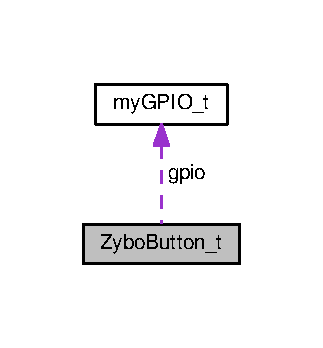
\includegraphics[width=155pt]{struct_zybo_button__t__coll__graph}
\end{center}
\end{figure}
\subsection*{Campi}
\begin{DoxyCompactItemize}
\item 
\hyperlink{structmy_g_p_i_o__t}{my\+G\+P\+I\+O\+\_\+t} $\ast$ \hyperlink{struct_zybo_button__t_ac37ddc7c58d246d233dfb38037020184}{gpio}
\item 
\hyperlink{group__bare-metal_ga402a0d20afc0cb7c25554b8b023f4253}{my\+G\+P\+I\+O\+\_\+mask} \hyperlink{struct_zybo_button__t_ad462a15a55883fd4c86d2be9e11968a7}{Button3\+\_\+pin}
\item 
\hyperlink{group__bare-metal_ga402a0d20afc0cb7c25554b8b023f4253}{my\+G\+P\+I\+O\+\_\+mask} \hyperlink{struct_zybo_button__t_a3b4fe634c2d98ce55fdef526c2d230d1}{Button2\+\_\+pin}
\item 
\hyperlink{group__bare-metal_ga402a0d20afc0cb7c25554b8b023f4253}{my\+G\+P\+I\+O\+\_\+mask} \hyperlink{struct_zybo_button__t_a6cb60bb285e32e29c51c15e85206aaeb}{Button1\+\_\+pin}
\item 
\hyperlink{group__bare-metal_ga402a0d20afc0cb7c25554b8b023f4253}{my\+G\+P\+I\+O\+\_\+mask} \hyperlink{struct_zybo_button__t_af7d7d5a9c9fc174e8f4ee4c762c2abee}{Button0\+\_\+pin}
\end{DoxyCompactItemize}


\subsection{Descrizione dettagliata}
Struttura opaca che astrae l'insieme dei button presenti sulla board Digilent Zybo;. \begin{Desc}
\item[Esempi\+: ]\par
\hyperlink{bsp_example_8c-example}{bsp\+\_\+example.\+c}.\end{Desc}


\subsection{Documentazione dei campi}
\hypertarget{struct_zybo_button__t_af7d7d5a9c9fc174e8f4ee4c762c2abee}{\index{Zybo\+Button\+\_\+t@{Zybo\+Button\+\_\+t}!Button0\+\_\+pin@{Button0\+\_\+pin}}
\index{Button0\+\_\+pin@{Button0\+\_\+pin}!Zybo\+Button\+\_\+t@{Zybo\+Button\+\_\+t}}
\subsubsection[{Button0\+\_\+pin}]{\setlength{\rightskip}{0pt plus 5cm}{\bf my\+G\+P\+I\+O\+\_\+mask} Button0\+\_\+pin}}\label{struct_zybo_button__t_af7d7d5a9c9fc174e8f4ee4c762c2abee}
maschera di selezione per il particolare bit del device my\+G\+P\+I\+O connesso al button numero 0 della board Zybo \hypertarget{struct_zybo_button__t_a6cb60bb285e32e29c51c15e85206aaeb}{\index{Zybo\+Button\+\_\+t@{Zybo\+Button\+\_\+t}!Button1\+\_\+pin@{Button1\+\_\+pin}}
\index{Button1\+\_\+pin@{Button1\+\_\+pin}!Zybo\+Button\+\_\+t@{Zybo\+Button\+\_\+t}}
\subsubsection[{Button1\+\_\+pin}]{\setlength{\rightskip}{0pt plus 5cm}{\bf my\+G\+P\+I\+O\+\_\+mask} Button1\+\_\+pin}}\label{struct_zybo_button__t_a6cb60bb285e32e29c51c15e85206aaeb}
maschera di selezione per il particolare bit del device my\+G\+P\+I\+O connesso al button numero 1 della board Zybo \hypertarget{struct_zybo_button__t_a3b4fe634c2d98ce55fdef526c2d230d1}{\index{Zybo\+Button\+\_\+t@{Zybo\+Button\+\_\+t}!Button2\+\_\+pin@{Button2\+\_\+pin}}
\index{Button2\+\_\+pin@{Button2\+\_\+pin}!Zybo\+Button\+\_\+t@{Zybo\+Button\+\_\+t}}
\subsubsection[{Button2\+\_\+pin}]{\setlength{\rightskip}{0pt plus 5cm}{\bf my\+G\+P\+I\+O\+\_\+mask} Button2\+\_\+pin}}\label{struct_zybo_button__t_a3b4fe634c2d98ce55fdef526c2d230d1}
maschera di selezione per il particolare bit del device my\+G\+P\+I\+O connesso al button numero 2 della board Zybo \hypertarget{struct_zybo_button__t_ad462a15a55883fd4c86d2be9e11968a7}{\index{Zybo\+Button\+\_\+t@{Zybo\+Button\+\_\+t}!Button3\+\_\+pin@{Button3\+\_\+pin}}
\index{Button3\+\_\+pin@{Button3\+\_\+pin}!Zybo\+Button\+\_\+t@{Zybo\+Button\+\_\+t}}
\subsubsection[{Button3\+\_\+pin}]{\setlength{\rightskip}{0pt plus 5cm}{\bf my\+G\+P\+I\+O\+\_\+mask} Button3\+\_\+pin}}\label{struct_zybo_button__t_ad462a15a55883fd4c86d2be9e11968a7}
maschera di selezione per il particolare bit del device my\+G\+P\+I\+O connesso al button numero 3 della board Zybo \hypertarget{struct_zybo_button__t_ac37ddc7c58d246d233dfb38037020184}{\index{Zybo\+Button\+\_\+t@{Zybo\+Button\+\_\+t}!gpio@{gpio}}
\index{gpio@{gpio}!Zybo\+Button\+\_\+t@{Zybo\+Button\+\_\+t}}
\subsubsection[{gpio}]{\setlength{\rightskip}{0pt plus 5cm}{\bf my\+G\+P\+I\+O\+\_\+t}$\ast$ gpio}}\label{struct_zybo_button__t_ac37ddc7c58d246d233dfb38037020184}
puntatore a struttura \hyperlink{structmy_g_p_i_o__t}{my\+G\+P\+I\+O\+\_\+t}, che astrae il particolare my\+G\+P\+I\+O usato per la lettura dello stato dei button presenti sulla board 

La documentazione per questa struct è stata generata a partire dal seguente file\+:\begin{DoxyCompactItemize}
\item 
Src/my\+G\+P\+I\+O/bare-\/metal/\+Zybo\+B\+S\+P/\hyperlink{_zybo_button_8h}{Zybo\+Button.\+h}\end{DoxyCompactItemize}

\hypertarget{struct_zybo_led__t}{\section{Riferimenti per la struct Zybo\+Led\+\_\+t}
\label{struct_zybo_led__t}\index{Zybo\+Led\+\_\+t@{Zybo\+Led\+\_\+t}}
}


Struttura opaca che astrae l'insieme dei Led presenti sulla board Digilent Zybo;.  




{\ttfamily \#include $<$Zybo\+Led.\+h$>$}



Diagramma di collaborazione per Zybo\+Led\+\_\+t\+:
\nopagebreak
\begin{figure}[H]
\begin{center}
\leavevmode
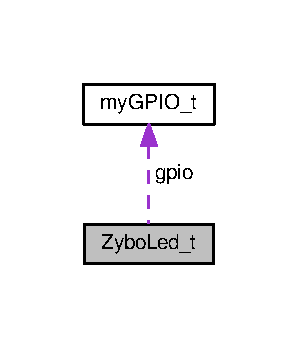
\includegraphics[width=143pt]{struct_zybo_led__t__coll__graph}
\end{center}
\end{figure}
\subsection*{Campi}
\begin{DoxyCompactItemize}
\item 
\hyperlink{structmy_g_p_i_o__t}{my\+G\+P\+I\+O\+\_\+t} $\ast$ \hyperlink{struct_zybo_led__t_ac37ddc7c58d246d233dfb38037020184}{gpio}
\item 
\hyperlink{group__my_g_p_i_o_ga402a0d20afc0cb7c25554b8b023f4253}{my\+G\+P\+I\+O\+\_\+mask} \hyperlink{struct_zybo_led__t_afc64d1407f30615e374bf9f06721842a}{Led3\+\_\+pin}
\item 
\hyperlink{group__my_g_p_i_o_ga402a0d20afc0cb7c25554b8b023f4253}{my\+G\+P\+I\+O\+\_\+mask} \hyperlink{struct_zybo_led__t_a4213c78e5a02b1476222e989c2eceb04}{Led2\+\_\+pin}
\item 
\hyperlink{group__my_g_p_i_o_ga402a0d20afc0cb7c25554b8b023f4253}{my\+G\+P\+I\+O\+\_\+mask} \hyperlink{struct_zybo_led__t_adc78fb167f1dd6693910813d4ec5930e}{Led1\+\_\+pin}
\item 
\hyperlink{group__my_g_p_i_o_ga402a0d20afc0cb7c25554b8b023f4253}{my\+G\+P\+I\+O\+\_\+mask} \hyperlink{struct_zybo_led__t_ac5afef2eef91d5533a23435cfcc60104}{Led0\+\_\+pin}
\end{DoxyCompactItemize}


\subsection{Descrizione dettagliata}
Struttura opaca che astrae l'insieme dei Led presenti sulla board Digilent Zybo;. 

\subsection{Documentazione dei campi}
\hypertarget{struct_zybo_led__t_ac37ddc7c58d246d233dfb38037020184}{\index{Zybo\+Led\+\_\+t@{Zybo\+Led\+\_\+t}!gpio@{gpio}}
\index{gpio@{gpio}!Zybo\+Led\+\_\+t@{Zybo\+Led\+\_\+t}}
\subsubsection[{gpio}]{\setlength{\rightskip}{0pt plus 5cm}{\bf my\+G\+P\+I\+O\+\_\+t}$\ast$ gpio}}\label{struct_zybo_led__t_ac37ddc7c58d246d233dfb38037020184}
puntatore a struttura \hyperlink{structmy_g_p_i_o__t}{my\+G\+P\+I\+O\+\_\+t}, che astrae il particolare G\+P\+I\+O usato per il pilotaggio dei led presenti sulla board \hypertarget{struct_zybo_led__t_ac5afef2eef91d5533a23435cfcc60104}{\index{Zybo\+Led\+\_\+t@{Zybo\+Led\+\_\+t}!Led0\+\_\+pin@{Led0\+\_\+pin}}
\index{Led0\+\_\+pin@{Led0\+\_\+pin}!Zybo\+Led\+\_\+t@{Zybo\+Led\+\_\+t}}
\subsubsection[{Led0\+\_\+pin}]{\setlength{\rightskip}{0pt plus 5cm}{\bf my\+G\+P\+I\+O\+\_\+mask} Led0\+\_\+pin}}\label{struct_zybo_led__t_ac5afef2eef91d5533a23435cfcc60104}
maschera di selezione per il particolare bit del device G\+P\+I\+O usato per il pilotaggio del led numero 0 della board Zybo \hypertarget{struct_zybo_led__t_adc78fb167f1dd6693910813d4ec5930e}{\index{Zybo\+Led\+\_\+t@{Zybo\+Led\+\_\+t}!Led1\+\_\+pin@{Led1\+\_\+pin}}
\index{Led1\+\_\+pin@{Led1\+\_\+pin}!Zybo\+Led\+\_\+t@{Zybo\+Led\+\_\+t}}
\subsubsection[{Led1\+\_\+pin}]{\setlength{\rightskip}{0pt plus 5cm}{\bf my\+G\+P\+I\+O\+\_\+mask} Led1\+\_\+pin}}\label{struct_zybo_led__t_adc78fb167f1dd6693910813d4ec5930e}
maschera di selezione per il particolare bit del device G\+P\+I\+O usato per il pilotaggio del led numero 1 della board Zybo \hypertarget{struct_zybo_led__t_a4213c78e5a02b1476222e989c2eceb04}{\index{Zybo\+Led\+\_\+t@{Zybo\+Led\+\_\+t}!Led2\+\_\+pin@{Led2\+\_\+pin}}
\index{Led2\+\_\+pin@{Led2\+\_\+pin}!Zybo\+Led\+\_\+t@{Zybo\+Led\+\_\+t}}
\subsubsection[{Led2\+\_\+pin}]{\setlength{\rightskip}{0pt plus 5cm}{\bf my\+G\+P\+I\+O\+\_\+mask} Led2\+\_\+pin}}\label{struct_zybo_led__t_a4213c78e5a02b1476222e989c2eceb04}
maschera di selezione per il particolare bit del device G\+P\+I\+O usato per il pilotaggio del led numero 2 della board Zybo \hypertarget{struct_zybo_led__t_afc64d1407f30615e374bf9f06721842a}{\index{Zybo\+Led\+\_\+t@{Zybo\+Led\+\_\+t}!Led3\+\_\+pin@{Led3\+\_\+pin}}
\index{Led3\+\_\+pin@{Led3\+\_\+pin}!Zybo\+Led\+\_\+t@{Zybo\+Led\+\_\+t}}
\subsubsection[{Led3\+\_\+pin}]{\setlength{\rightskip}{0pt plus 5cm}{\bf my\+G\+P\+I\+O\+\_\+mask} Led3\+\_\+pin}}\label{struct_zybo_led__t_afc64d1407f30615e374bf9f06721842a}
maschera di selezione per il particolare bit del device G\+P\+I\+O usato per il pilotaggio del led numero 3 della board Zybo 

La documentazione per questa struct è stata generata a partire dal seguente file\+:\begin{DoxyCompactItemize}
\item 
Zybo/\hyperlink{_zybo_led_8h}{Zybo\+Led.\+h}\end{DoxyCompactItemize}

\hypertarget{struct_zybo_switch__t}{\section{Riferimenti per la struct Zybo\+Switch\+\_\+t}
\label{struct_zybo_switch__t}\index{Zybo\+Switch\+\_\+t@{Zybo\+Switch\+\_\+t}}
}


Struttura opaca che astrae l'insieme degli switch presenti sulla board Digilent Zybo;.  




{\ttfamily \#include $<$Zybo\+Switch.\+h$>$}



Diagramma di collaborazione per Zybo\+Switch\+\_\+t\+:
\nopagebreak
\begin{figure}[H]
\begin{center}
\leavevmode
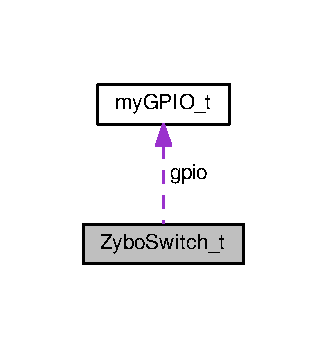
\includegraphics[width=157pt]{struct_zybo_switch__t__coll__graph}
\end{center}
\end{figure}
\subsection*{Campi}
\begin{DoxyCompactItemize}
\item 
\hypertarget{struct_zybo_switch__t_acb3116190992a4d8d26545c103304d27}{\hyperlink{struct_g_p_i_o__t}{G\+P\+I\+O\+\_\+t} $\ast$ {\bfseries gpio}}\label{struct_zybo_switch__t_acb3116190992a4d8d26545c103304d27}

\item 
\hypertarget{struct_zybo_switch__t_a6b95420b88fe8c1fd7f347ce3ae1906b}{G\+P\+I\+O\+\_\+mask {\bfseries Switch3\+\_\+pin}}\label{struct_zybo_switch__t_a6b95420b88fe8c1fd7f347ce3ae1906b}

\item 
\hypertarget{struct_zybo_switch__t_a33eda4a0115ef585edd90078924ca56e}{G\+P\+I\+O\+\_\+mask {\bfseries Switch2\+\_\+pin}}\label{struct_zybo_switch__t_a33eda4a0115ef585edd90078924ca56e}

\item 
\hypertarget{struct_zybo_switch__t_a6a3a5739e7e8f138241cafeeb7c1a33f}{G\+P\+I\+O\+\_\+mask {\bfseries Switch1\+\_\+pin}}\label{struct_zybo_switch__t_a6a3a5739e7e8f138241cafeeb7c1a33f}

\item 
\hypertarget{struct_zybo_switch__t_a5b7f83cd96441b7d1692710c6499147c}{G\+P\+I\+O\+\_\+mask {\bfseries Switch0\+\_\+pin}}\label{struct_zybo_switch__t_a5b7f83cd96441b7d1692710c6499147c}

\end{DoxyCompactItemize}


\subsection{Descrizione dettagliata}
Struttura opaca che astrae l'insieme degli switch presenti sulla board Digilent Zybo;. 

La documentazione per questa struct è stata generata a partire dal seguente file\+:\begin{DoxyCompactItemize}
\item 
Zybo/Zybo\+Switch.\+h\end{DoxyCompactItemize}

\chapter{Documentazione dei file}
\hypertarget{my_g_p_i_o_8c}{\section{Riferimenti per il file Src/my\+G\+P\+I\+O/bare-\/metal/my\+G\+P\+I\+O.c}
\label{my_g_p_i_o_8c}\index{Src/my\+G\+P\+I\+O/bare-\/metal/my\+G\+P\+I\+O.\+c@{Src/my\+G\+P\+I\+O/bare-\/metal/my\+G\+P\+I\+O.\+c}}
}
{\ttfamily \#include \char`\"{}my\+G\+P\+I\+O.\+h\char`\"{}}\\*
{\ttfamily \#include $<$stdlib.\+h$>$}\\*
{\ttfamily \#include $<$assert.\+h$>$}\\*
Grafo delle dipendenze di inclusione per my\+G\+P\+I\+O.\+c\+:\nopagebreak
\begin{figure}[H]
\begin{center}
\leavevmode
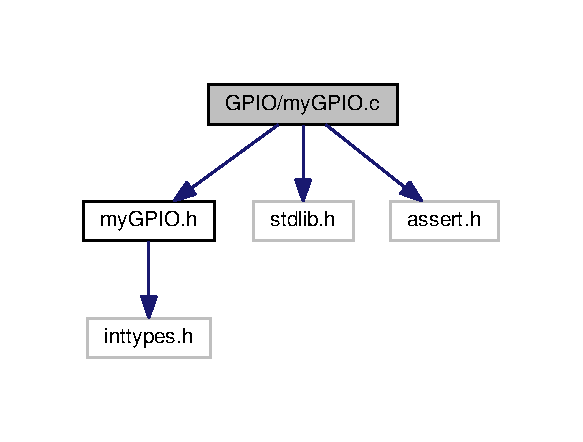
\includegraphics[width=280pt]{my_g_p_i_o_8c__incl}
\end{center}
\end{figure}
\subsection*{Funzioni}
\begin{DoxyCompactItemize}
\item 
void \hyperlink{group__bare-metal_ga588201358d1633c53535b288c9198531}{my\+G\+P\+I\+O\+\_\+\+Init} (\hyperlink{structmy_g_p_i_o__t}{my\+G\+P\+I\+O\+\_\+t} $\ast$gpio, uint32\+\_\+t base\+\_\+address)
\begin{DoxyCompactList}\small\item\em Inizializza un device my\+G\+P\+I\+O. \end{DoxyCompactList}\item 
void \hyperlink{group__bare-metal_ga43e82eb0febd452635a438fbd9cb853b}{my\+G\+P\+I\+O\+\_\+\+Set\+Mode} (\hyperlink{structmy_g_p_i_o__t}{my\+G\+P\+I\+O\+\_\+t} $\ast$gpio, \hyperlink{group__bare-metal_ga402a0d20afc0cb7c25554b8b023f4253}{my\+G\+P\+I\+O\+\_\+mask} mask, \hyperlink{group__bare-metal_ga76b849f0e0c05e7f9161bdb33396f2b1}{my\+G\+P\+I\+O\+\_\+mode} mode)
\begin{DoxyCompactList}\small\item\em Permette di settare la modalita' lettura/scrittura dei pin di un device my\+G\+P\+I\+O;. \end{DoxyCompactList}\item 
void \hyperlink{group__bare-metal_ga9d9ce9d2db7d77a588da4a3749f2f24d}{my\+G\+P\+I\+O\+\_\+\+Set\+Value} (\hyperlink{structmy_g_p_i_o__t}{my\+G\+P\+I\+O\+\_\+t} $\ast$gpio, \hyperlink{group__bare-metal_ga402a0d20afc0cb7c25554b8b023f4253}{my\+G\+P\+I\+O\+\_\+mask} mask, \hyperlink{group__bare-metal_gaf634fe4a0e1eab8da5000b72d6ad362b}{my\+G\+P\+I\+O\+\_\+value} value)
\begin{DoxyCompactList}\small\item\em Permette di settare il valore dei pin di un device my\+G\+P\+I\+O, se configurati come output. \end{DoxyCompactList}\item 
void \hyperlink{group__bare-metal_ga449b2af7cc20d24e6f6e017cf792ce03}{my\+G\+P\+I\+O\+\_\+\+Toggle} (\hyperlink{structmy_g_p_i_o__t}{my\+G\+P\+I\+O\+\_\+t} $\ast$gpio, \hyperlink{group__bare-metal_ga402a0d20afc0cb7c25554b8b023f4253}{my\+G\+P\+I\+O\+\_\+mask} mask)
\begin{DoxyCompactList}\small\item\em Permette di invertire il valore dei pin di un device my\+G\+P\+I\+O, se configurati come output. \end{DoxyCompactList}\item 
\hyperlink{group__bare-metal_gaf634fe4a0e1eab8da5000b72d6ad362b}{my\+G\+P\+I\+O\+\_\+value} \hyperlink{group__bare-metal_ga2a20e519816733b90204b975edc4e212}{my\+G\+P\+I\+O\+\_\+\+Get\+Value} (\hyperlink{structmy_g_p_i_o__t}{my\+G\+P\+I\+O\+\_\+t} $\ast$gpio, \hyperlink{group__bare-metal_ga402a0d20afc0cb7c25554b8b023f4253}{my\+G\+P\+I\+O\+\_\+mask} mask)
\begin{DoxyCompactList}\small\item\em Permette di leggere il valore dei pin di un device my\+G\+P\+I\+O;. \end{DoxyCompactList}\item 
\hyperlink{group__bare-metal_ga402a0d20afc0cb7c25554b8b023f4253}{my\+G\+P\+I\+O\+\_\+mask} \hyperlink{group__bare-metal_gac35776cd6652f7b932a132f3f6959a11}{my\+G\+P\+I\+O\+\_\+\+Get\+Read} (\hyperlink{structmy_g_p_i_o__t}{my\+G\+P\+I\+O\+\_\+t} $\ast$gpio)
\begin{DoxyCompactList}\small\item\em Restituisce la maschera dei pin settati di un device my\+G\+P\+I\+O. \end{DoxyCompactList}\item 
void \hyperlink{group__bare-metal_gada93ef6a9818e634f0a233ce14582216}{my\+G\+P\+I\+O\+\_\+\+Global\+Interrupt\+Enable} (\hyperlink{structmy_g_p_i_o__t}{my\+G\+P\+I\+O\+\_\+t} $\ast$gpio)
\begin{DoxyCompactList}\small\item\em Abilita gli interrupt globali;. \end{DoxyCompactList}\item 
void \hyperlink{group__bare-metal_gaacca2871ac57a166e62bf431a2da7548}{my\+G\+P\+I\+O\+\_\+\+Global\+Interrupt\+Disable} (\hyperlink{structmy_g_p_i_o__t}{my\+G\+P\+I\+O\+\_\+t} $\ast$gpio)
\begin{DoxyCompactList}\small\item\em Disabilita gli interrupt globali;. \end{DoxyCompactList}\item 
\hyperlink{group__bare-metal_gaf634fe4a0e1eab8da5000b72d6ad362b}{my\+G\+P\+I\+O\+\_\+value} \hyperlink{group__bare-metal_ga0a753db3d02ad08014e4b7304e0f1829}{my\+G\+P\+I\+O\+\_\+\+Is\+Global\+Interrupt\+Enabled} (\hyperlink{structmy_g_p_i_o__t}{my\+G\+P\+I\+O\+\_\+t} $\ast$gpio)
\begin{DoxyCompactList}\small\item\em Consente di verificare se gli interrupt globali siano abilitati. \end{DoxyCompactList}\item 
\hyperlink{group__bare-metal_gaf634fe4a0e1eab8da5000b72d6ad362b}{my\+G\+P\+I\+O\+\_\+value} \hyperlink{group__bare-metal_ga386cea84aca8c6bb731b4b46fcbf9199}{my\+G\+P\+I\+O\+\_\+\+Pending\+Interrupt} (\hyperlink{structmy_g_p_i_o__t}{my\+G\+P\+I\+O\+\_\+t} $\ast$gpio)
\begin{DoxyCompactList}\small\item\em Consente di verificare se esistano interrupt non ancora serviti. \end{DoxyCompactList}\item 
void \hyperlink{group__bare-metal_ga116e3a1077a317e9e42ded6dd4df64af}{my\+G\+P\+I\+O\+\_\+\+Pin\+Interrupt\+Enable} (\hyperlink{structmy_g_p_i_o__t}{my\+G\+P\+I\+O\+\_\+t} $\ast$gpio, \hyperlink{group__bare-metal_ga402a0d20afc0cb7c25554b8b023f4253}{my\+G\+P\+I\+O\+\_\+mask} mask)
\begin{DoxyCompactList}\small\item\em Abilita gli interrupt per i singoli pin del device. \end{DoxyCompactList}\item 
void \hyperlink{group__bare-metal_ga37d3df33ac50387d6f2e1fb5e2b13e49}{my\+G\+P\+I\+O\+\_\+\+Pin\+Interrupt\+Disable} (\hyperlink{structmy_g_p_i_o__t}{my\+G\+P\+I\+O\+\_\+t} $\ast$gpio, \hyperlink{group__bare-metal_ga402a0d20afc0cb7c25554b8b023f4253}{my\+G\+P\+I\+O\+\_\+mask} mask)
\begin{DoxyCompactList}\small\item\em Disabilita gli interrupt per i singoli pin del device. \end{DoxyCompactList}\item 
\hyperlink{group__bare-metal_ga402a0d20afc0cb7c25554b8b023f4253}{my\+G\+P\+I\+O\+\_\+mask} \hyperlink{group__bare-metal_ga80ef1cf3e9bd8bfd4d849a0f3b8e7b2c}{my\+G\+P\+I\+O\+\_\+\+Enabled\+Pin\+Interrupt} (\hyperlink{structmy_g_p_i_o__t}{my\+G\+P\+I\+O\+\_\+t} $\ast$gpio)
\begin{DoxyCompactList}\small\item\em Consente di ottenere una maschera che indichi quali pin abbiano interrupt abilitati. \end{DoxyCompactList}\item 
\hyperlink{group__bare-metal_ga402a0d20afc0cb7c25554b8b023f4253}{my\+G\+P\+I\+O\+\_\+mask} \hyperlink{group__bare-metal_ga6115bde39f860d4e76e7d8f421ce222c}{my\+G\+P\+I\+O\+\_\+\+Pending\+Pin\+Interrupt} (\hyperlink{structmy_g_p_i_o__t}{my\+G\+P\+I\+O\+\_\+t} $\ast$gpio)
\begin{DoxyCompactList}\small\item\em Consente di ottenere una maschera che indichi quali interrupt non siano stati ancora serviti;. \end{DoxyCompactList}\item 
void \hyperlink{group__bare-metal_gab6ad3dda867515825890c97dbf6f55db}{my\+G\+P\+I\+O\+\_\+\+Pin\+Interrupt\+Ack} (\hyperlink{structmy_g_p_i_o__t}{my\+G\+P\+I\+O\+\_\+t} $\ast$gpio, \hyperlink{group__bare-metal_ga402a0d20afc0cb7c25554b8b023f4253}{my\+G\+P\+I\+O\+\_\+mask} mask)
\begin{DoxyCompactList}\small\item\em Invia al device notifica di servizio di un interrupt;. \end{DoxyCompactList}\end{DoxyCompactItemize}


\subsection{Descrizione dettagliata}
\begin{DoxyAuthor}{Autore}
\+: Salvatore Barone \href{mailto:salvator.barone@gmail.com}{\tt salvator.\+barone@gmail.\+com} 
\end{DoxyAuthor}
\begin{DoxyDate}{Data}
\+: 12 05 2017
\end{DoxyDate}
\begin{DoxyCopyright}{Copyright}
Copyright 2017 Salvatore Barone \href{mailto:salvator.barone@gmail.com}{\tt salvator.\+barone@gmail.\+com}
\end{DoxyCopyright}
This file is part of Zynq7000\+Driver\+Pack

Zynq7000\+Driver\+Pack is free software; you can redistribute it and/or modify it under the terms of the G\+N\+U General Public License as published by the Free Software Foundation; either version 3 of the License, or any later version.

Zynq7000\+Driver\+Pack is distributed in the hope that it will be useful, but W\+I\+T\+H\+O\+U\+T A\+N\+Y W\+A\+R\+R\+A\+N\+T\+Y; without even the implied warranty of M\+E\+R\+C\+H\+A\+N\+T\+A\+B\+I\+L\+I\+T\+Y or F\+I\+T\+N\+E\+S\+S F\+O\+R A P\+A\+R\+T\+I\+C\+U\+L\+A\+R P\+U\+R\+P\+O\+S\+E. See the G\+N\+U General Public License for more details.

You should have received a copy of the G\+N\+U General Public License along with this program; if not, write to the Free Software Foundation, Inc., 51 Franklin Street, Fifth Floor, Boston, M\+A 02110-\/1301, U\+S\+A. 
\hypertarget{my_g_p_i_o_8h}{\section{Riferimenti per il file my\+G\+P\+I\+O/my\+G\+P\+I\+O.h}
\label{my_g_p_i_o_8h}\index{my\+G\+P\+I\+O/my\+G\+P\+I\+O.\+h@{my\+G\+P\+I\+O/my\+G\+P\+I\+O.\+h}}
}
{\ttfamily \#include $<$inttypes.\+h$>$}\\*
Grafo delle dipendenze di inclusione per my\+G\+P\+I\+O.\+h\+:\nopagebreak
\begin{figure}[H]
\begin{center}
\leavevmode
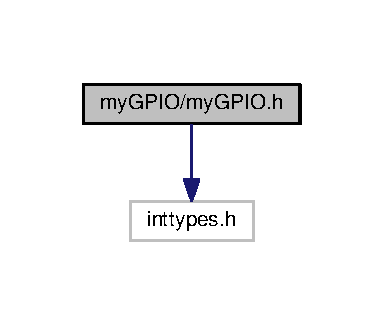
\includegraphics[width=184pt]{my_g_p_i_o_8h__incl}
\end{center}
\end{figure}
Questo grafo mostra quali altri file includono direttamente o indirettamente questo file\+:\nopagebreak
\begin{figure}[H]
\begin{center}
\leavevmode
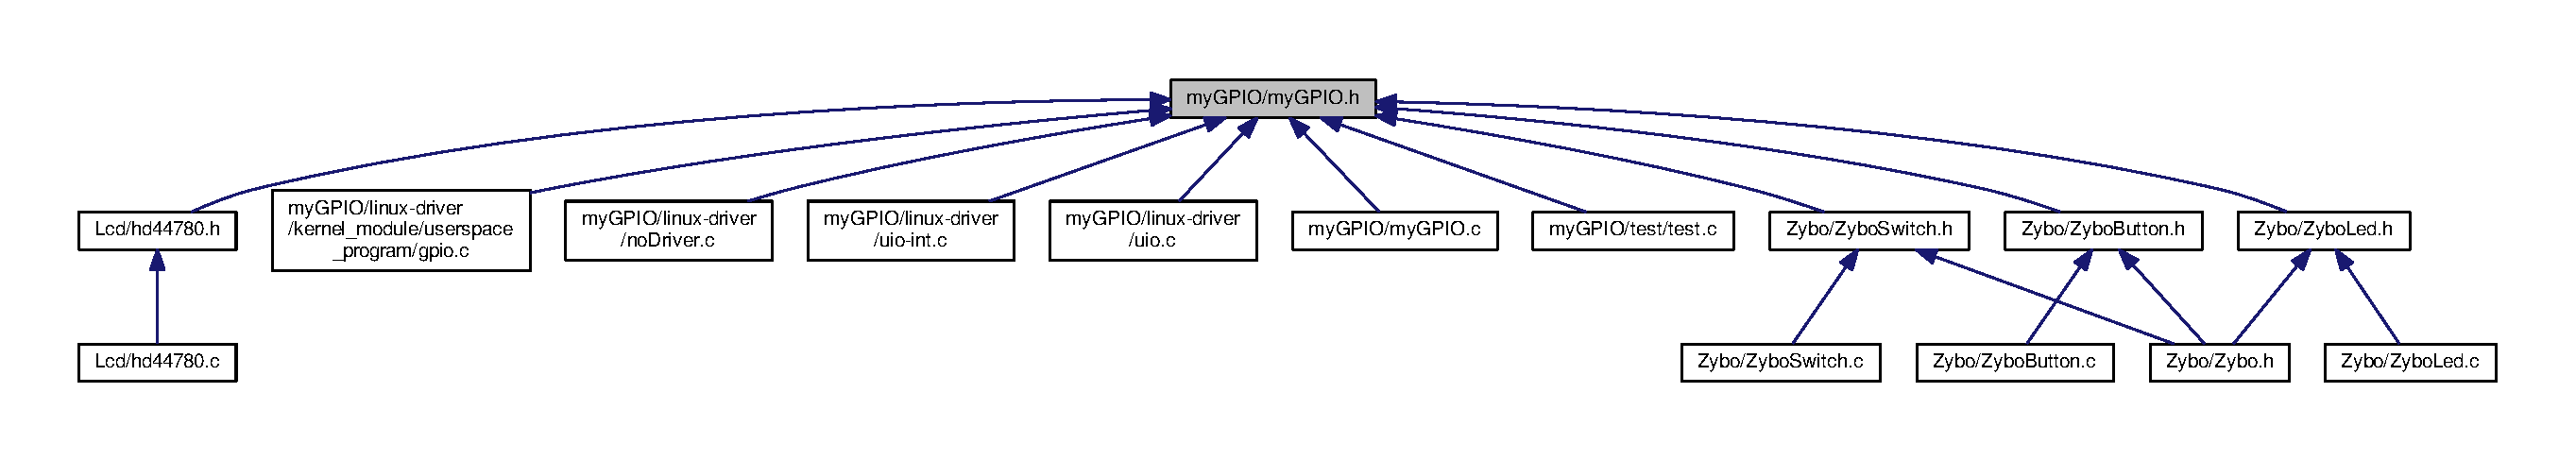
\includegraphics[width=350pt]{my_g_p_i_o_8h__dep__incl}
\end{center}
\end{figure}
\subsection*{Strutture dati}
\begin{DoxyCompactItemize}
\item 
struct \hyperlink{structmy_g_p_i_o__t}{my\+G\+P\+I\+O\+\_\+t}
\begin{DoxyCompactList}\small\item\em Struttura che astrae un device my\+G\+P\+I\+O. \end{DoxyCompactList}\end{DoxyCompactItemize}
\subsection*{Definizioni}
\begin{DoxyCompactItemize}
\item 
\#define \hyperlink{group__my_g_p_i_o_ga81a662103d6ed053978c0a9b4c273065}{my\+G\+P\+I\+O\+\_\+\+M\+O\+D\+E\+\_\+\+O\+F\+F\+S\+E\+T}~0\+U
\begin{DoxyCompactList}\small\item\em Offset, rispetto all'indirizzo base, del registro \char`\"{}mode\char`\"{} per il device my\+G\+P\+I\+O. \end{DoxyCompactList}\item 
\#define \hyperlink{group__my_g_p_i_o_ga2e45778b6ca9ce6f5768b3f7a4557ce1}{my\+G\+P\+I\+O\+\_\+\+W\+R\+I\+T\+E\+\_\+\+O\+F\+F\+S\+E\+T}~4\+U
\begin{DoxyCompactList}\small\item\em Offset, rispetto all'indirizzo base, del registro \char`\"{}write\char`\"{} per il device my\+G\+P\+I\+O. \end{DoxyCompactList}\item 
\#define \hyperlink{group__my_g_p_i_o_ga584d2dfece76e5762030d918d80592cc}{my\+G\+P\+I\+O\+\_\+\+R\+E\+A\+D\+\_\+\+O\+F\+F\+S\+E\+T}~8\+U
\begin{DoxyCompactList}\small\item\em Offset, rispetto all'indirizzo base, del registro \char`\"{}read\char`\"{} per il device my\+G\+P\+I\+O. \end{DoxyCompactList}\item 
\#define \hyperlink{group__my_g_p_i_o_gaacf2d8a21a051e778f02f8811b9c1e96}{my\+G\+P\+I\+O\+\_\+\+I\+N\+T\+R\+\_\+\+O\+F\+F\+S\+E\+T}~12\+U
\begin{DoxyCompactList}\small\item\em Offset, rispetto all'indirizzo base, del registro \char`\"{}interrupt\char`\"{} per il device my\+G\+P\+I\+O. \end{DoxyCompactList}\item 
\#define \hyperlink{group__my_g_p_i_o_ga0ba32e2adf874ed7216c5993369153e1}{my\+G\+P\+I\+O\+\_\+\+I\+N\+T\+R\+\_\+\+Int\+En\+\_\+mask}~0x1\+U
\begin{DoxyCompactList}\small\item\em maschera del bit del registro \char`\"{}interrupt\char`\"{} che funge da interrupt-\/enable, per il device my\+G\+P\+I\+O \end{DoxyCompactList}\item 
\#define \hyperlink{group__my_g_p_i_o_ga4cd02635783bc2a4ad7639cfb9fdb698}{my\+G\+P\+I\+O\+\_\+\+I\+N\+T\+R\+\_\+\+Irq\+\_\+mask}~0x2\+U
\begin{DoxyCompactList}\small\item\em maschera del bit del registro \char`\"{}interrupt\char`\"{} che funge da interrupt-\/request, per il device my\+G\+P\+I\+O \end{DoxyCompactList}\item 
\#define \hyperlink{group__my_g_p_i_o_gaa760b8397e6372e48c1008c2ba8d7387}{my\+G\+P\+I\+O\+\_\+\+I\+N\+T\+R\+\_\+\+Int\+Ack\+\_\+mask}~0x4\+U
\begin{DoxyCompactList}\small\item\em maschera del bit del registro \char`\"{}interrupt\char`\"{} che funge da interrupt-\/ack, per il device my\+G\+P\+I\+O \end{DoxyCompactList}\item 
\#define \hyperlink{group__my_g_p_i_o_gabbe2491a3b71c292521025b7b382b971}{my\+G\+P\+I\+O\+\_\+pin}(i)~((uint32\+\_\+t)(1$<$$<$(i)))
\begin{DoxyCompactList}\small\item\em Metodo alternativo per la specifica di uno dei pin di un device my\+G\+P\+I\+O. \end{DoxyCompactList}\end{DoxyCompactItemize}
\subsection*{Tipi enumerati (enum)}
\begin{DoxyCompactItemize}
\item 
enum \hyperlink{group__my_g_p_i_o_ga402a0d20afc0cb7c25554b8b023f4253}{my\+G\+P\+I\+O\+\_\+mask} \{ \\*
\hyperlink{group__my_g_p_i_o_gga402a0d20afc0cb7c25554b8b023f4253a6db6fa7be955ae379f543d96122e23a9}{my\+G\+P\+I\+O\+\_\+pin0} = 0x1\+U, 
\hyperlink{group__my_g_p_i_o_gga402a0d20afc0cb7c25554b8b023f4253a1de6bdcc01efca2c39f584f5a20293be}{my\+G\+P\+I\+O\+\_\+pin1} = 0x2\+U, 
\hyperlink{group__my_g_p_i_o_gga402a0d20afc0cb7c25554b8b023f4253a1fb3f52d920ac8ba17b74dd73c27d783}{my\+G\+P\+I\+O\+\_\+pin2} = 0x4\+U, 
\hyperlink{group__my_g_p_i_o_gga402a0d20afc0cb7c25554b8b023f4253a4514d64390392b626aa4dbfaac8dc1e5}{my\+G\+P\+I\+O\+\_\+pin3} = 0x8\+U, 
\\*
\hyperlink{group__my_g_p_i_o_gga402a0d20afc0cb7c25554b8b023f4253a0a446f53dee6f6f4ccb9a1d1f947b637}{my\+G\+P\+I\+O\+\_\+pin4} = 0x10\+U, 
\hyperlink{group__my_g_p_i_o_gga402a0d20afc0cb7c25554b8b023f4253a04a111036a27e9b97f0950f6d37b04d2}{my\+G\+P\+I\+O\+\_\+pin5} = 0x20\+U, 
\hyperlink{group__my_g_p_i_o_gga402a0d20afc0cb7c25554b8b023f4253a39a529f8c0a4f302029f54daa815471b}{my\+G\+P\+I\+O\+\_\+pin6} = 0x40\+U, 
\hyperlink{group__my_g_p_i_o_gga402a0d20afc0cb7c25554b8b023f4253af4e88b077442e4c0f459e1e4aa60626b}{my\+G\+P\+I\+O\+\_\+pin7} = 0x80\+U, 
\\*
\hyperlink{group__my_g_p_i_o_gga402a0d20afc0cb7c25554b8b023f4253a615159bcf4e347dc2b60f2545fae5f9e}{my\+G\+P\+I\+O\+\_\+pin8} = 0x100\+U, 
\hyperlink{group__my_g_p_i_o_gga402a0d20afc0cb7c25554b8b023f4253a8d721236fb936126a08c12b87696f6e9}{my\+G\+P\+I\+O\+\_\+pin9} = 0x200\+U, 
\hyperlink{group__my_g_p_i_o_gga402a0d20afc0cb7c25554b8b023f4253ae3067b7b3b1a2e171ecd74b6abd48341}{my\+G\+P\+I\+O\+\_\+pin10} = 0x400\+U, 
\hyperlink{group__my_g_p_i_o_gga402a0d20afc0cb7c25554b8b023f4253ae5c2e65508bfd452100d9da331d6220a}{my\+G\+P\+I\+O\+\_\+pin11} = 0x800\+U, 
\\*
\hyperlink{group__my_g_p_i_o_gga402a0d20afc0cb7c25554b8b023f4253afa75e3c1c019048c8553cb733c5137b5}{my\+G\+P\+I\+O\+\_\+pin12} = 0x1000\+U, 
\hyperlink{group__my_g_p_i_o_gga402a0d20afc0cb7c25554b8b023f4253a243381a796f0936a576f184dd115b37c}{my\+G\+P\+I\+O\+\_\+pin13} = 0x2000\+U, 
\hyperlink{group__my_g_p_i_o_gga402a0d20afc0cb7c25554b8b023f4253aed4915d6b3eab49cc1ba971b9f439fdd}{my\+G\+P\+I\+O\+\_\+pin14} = 0x4000\+U, 
\hyperlink{group__my_g_p_i_o_gga402a0d20afc0cb7c25554b8b023f4253a46c427ea97182a77e8c975d3429a64ee}{my\+G\+P\+I\+O\+\_\+pin15} = 0x8000\+U, 
\\*
\hyperlink{group__my_g_p_i_o_gga402a0d20afc0cb7c25554b8b023f4253a5a27c4d87207b2eba865876854f1ba67}{my\+G\+P\+I\+O\+\_\+pin16} = 0x10000\+U, 
\hyperlink{group__my_g_p_i_o_gga402a0d20afc0cb7c25554b8b023f4253ab0541af31059bdc8dca44d5dafa7e779}{my\+G\+P\+I\+O\+\_\+pin17} = 0x20000\+U, 
\hyperlink{group__my_g_p_i_o_gga402a0d20afc0cb7c25554b8b023f4253a7a51a492e3cb580581a2c8eb439edd99}{my\+G\+P\+I\+O\+\_\+pin18} = 0x40000\+U, 
\hyperlink{group__my_g_p_i_o_gga402a0d20afc0cb7c25554b8b023f4253a9118ae2775e93bd4522660e81a2d5309}{my\+G\+P\+I\+O\+\_\+pin19} = 0x80000\+U, 
\\*
\hyperlink{group__my_g_p_i_o_gga402a0d20afc0cb7c25554b8b023f4253a7940782a16f88dbbb3a4037c2bef1711}{my\+G\+P\+I\+O\+\_\+pin20} = 0x100000\+U, 
\hyperlink{group__my_g_p_i_o_gga402a0d20afc0cb7c25554b8b023f4253a1da616a8cf4396927db1e5a336fb6dc5}{my\+G\+P\+I\+O\+\_\+pin21} = 0x200000\+U, 
\hyperlink{group__my_g_p_i_o_gga402a0d20afc0cb7c25554b8b023f4253acf80113da8d789f7da9f9edc4ab6003c}{my\+G\+P\+I\+O\+\_\+pin22} = 0x400000\+U, 
\hyperlink{group__my_g_p_i_o_gga402a0d20afc0cb7c25554b8b023f4253ad64e03b703608de173ab5950b5121830}{my\+G\+P\+I\+O\+\_\+pin23} = 0x800000\+U, 
\\*
\hyperlink{group__my_g_p_i_o_gga402a0d20afc0cb7c25554b8b023f4253a5bb93f546327123f81b06ed0dfcdf110}{my\+G\+P\+I\+O\+\_\+pin24} = 0x1000000\+U, 
\hyperlink{group__my_g_p_i_o_gga402a0d20afc0cb7c25554b8b023f4253a0b27a7e78aff5836f33085f3b4539f56}{my\+G\+P\+I\+O\+\_\+pin25} = 0x2000000\+U, 
\hyperlink{group__my_g_p_i_o_gga402a0d20afc0cb7c25554b8b023f4253aaa07c24140250dcbc695206793efa8af}{my\+G\+P\+I\+O\+\_\+pin26} = 0x4000000\+U, 
\hyperlink{group__my_g_p_i_o_gga402a0d20afc0cb7c25554b8b023f4253a1dd5e99eba6237aeb30b2194c553c37f}{my\+G\+P\+I\+O\+\_\+pin27} = 0x8000000\+U, 
\\*
\hyperlink{group__my_g_p_i_o_gga402a0d20afc0cb7c25554b8b023f4253a2076590efec8bcf9ef3285798753e632}{my\+G\+P\+I\+O\+\_\+pin28} = 0x10000000\+U, 
\hyperlink{group__my_g_p_i_o_gga402a0d20afc0cb7c25554b8b023f4253abfe9540fa3946a35e20f7f68cb1b8084}{my\+G\+P\+I\+O\+\_\+pin29} = 0x20000000\+U, 
\hyperlink{group__my_g_p_i_o_gga402a0d20afc0cb7c25554b8b023f4253a59993a30c537c116eddb42d10778f4f8}{my\+G\+P\+I\+O\+\_\+pin30} = 0x40000000\+U, 
\hyperlink{group__my_g_p_i_o_gga402a0d20afc0cb7c25554b8b023f4253a9a55b7c245bd9aad750b7891d27e9225}{my\+G\+P\+I\+O\+\_\+pin31} = 0x80000000\+U, 
\\*
\hyperlink{group__my_g_p_i_o_gga402a0d20afc0cb7c25554b8b023f4253a0347b1742eef6b2575a7d409c7fb5c3d}{my\+G\+P\+I\+O\+\_\+byte0} = 0x000000ff\+U, 
\hyperlink{group__my_g_p_i_o_gga402a0d20afc0cb7c25554b8b023f4253ae5aec65fa20f554b893e419fc2755fd0}{my\+G\+P\+I\+O\+\_\+byte1} = 0x0000ff00\+U, 
\hyperlink{group__my_g_p_i_o_gga402a0d20afc0cb7c25554b8b023f4253af4892f7db28c64a7cf2a7236c88b742b}{my\+G\+P\+I\+O\+\_\+byte2} = 0x00ff0000\+U, 
\hyperlink{group__my_g_p_i_o_gga402a0d20afc0cb7c25554b8b023f4253a1ceefb9d65397352e986c573984d0129}{my\+G\+P\+I\+O\+\_\+byte3} = 0xff000000\+U
 \}
\begin{DoxyCompactList}\small\item\em Maschere di selezione dei pin di un device my\+G\+P\+I\+O. \end{DoxyCompactList}\item 
enum \hyperlink{group__my_g_p_i_o_ga76b849f0e0c05e7f9161bdb33396f2b1}{my\+G\+P\+I\+O\+\_\+mode} \{ \hyperlink{group__my_g_p_i_o_gga76b849f0e0c05e7f9161bdb33396f2b1a1e6dc78e7641e878cadc842d39605d5d}{my\+G\+P\+I\+O\+\_\+read}, 
\hyperlink{group__my_g_p_i_o_gga76b849f0e0c05e7f9161bdb33396f2b1a2d66976280eb7595a42c631683bdfad6}{my\+G\+P\+I\+O\+\_\+write}
 \}
\begin{DoxyCompactList}\small\item\em my\+G\+P\+I\+O\+\_\+mode, modalita' di funzionamento (lettura/scrittura) di un device my\+G\+P\+I\+O \end{DoxyCompactList}\item 
enum \hyperlink{group__my_g_p_i_o_gaf634fe4a0e1eab8da5000b72d6ad362b}{my\+G\+P\+I\+O\+\_\+value} \{ \hyperlink{group__my_g_p_i_o_ggaf634fe4a0e1eab8da5000b72d6ad362ba98cde80dbda025bd1ae7231c76b55674}{my\+G\+P\+I\+O\+\_\+reset}, 
\hyperlink{group__my_g_p_i_o_ggaf634fe4a0e1eab8da5000b72d6ad362ba10d296f3711d01189cc6c2d87f7c9149}{my\+G\+P\+I\+O\+\_\+set}
 \}
\begin{DoxyCompactList}\small\item\em my\+G\+P\+I\+O\+\_\+value, valore di un my\+G\+P\+I\+O \end{DoxyCompactList}\end{DoxyCompactItemize}
\subsection*{Funzioni}
\begin{DoxyCompactItemize}
\item 
void \hyperlink{group__my_g_p_i_o_ga8fda7ca73b187baf256409423c25d725}{my\+G\+P\+I\+O\+\_\+init} (\hyperlink{structmy_g_p_i_o__t}{my\+G\+P\+I\+O\+\_\+t} $\ast$gpio, uint32\+\_\+t base\+\_\+address)
\begin{DoxyCompactList}\small\item\em Inizializza un device my\+G\+P\+I\+O. \end{DoxyCompactList}\item 
void \hyperlink{group__my_g_p_i_o_ga38a2ea04d07af50f7f570f0367594c8b}{my\+G\+P\+I\+O\+\_\+set\+Mode} (\hyperlink{structmy_g_p_i_o__t}{my\+G\+P\+I\+O\+\_\+t} $\ast$gpio, \hyperlink{group__my_g_p_i_o_ga402a0d20afc0cb7c25554b8b023f4253}{my\+G\+P\+I\+O\+\_\+mask} mask, \hyperlink{group__my_g_p_i_o_ga76b849f0e0c05e7f9161bdb33396f2b1}{my\+G\+P\+I\+O\+\_\+mode} mode)
\begin{DoxyCompactList}\small\item\em Permette di settare la modalita' lettura/scrittura dei pin di un device my\+G\+P\+I\+O;. \end{DoxyCompactList}\item 
void \hyperlink{group__my_g_p_i_o_gab742e68093ad4c90fe299b64fd6736ca}{my\+G\+P\+I\+O\+\_\+set\+Value} (\hyperlink{structmy_g_p_i_o__t}{my\+G\+P\+I\+O\+\_\+t} $\ast$gpio, \hyperlink{group__my_g_p_i_o_ga402a0d20afc0cb7c25554b8b023f4253}{my\+G\+P\+I\+O\+\_\+mask} mask, \hyperlink{group__my_g_p_i_o_gaf634fe4a0e1eab8da5000b72d6ad362b}{my\+G\+P\+I\+O\+\_\+value} value)
\begin{DoxyCompactList}\small\item\em Permette di settare il valore dei pin di un device my\+G\+P\+I\+O, se configurati come output. \end{DoxyCompactList}\item 
void \hyperlink{group__my_g_p_i_o_ga27ea411bf51a58fe48eb8c5036780b53}{my\+G\+P\+I\+O\+\_\+toggle} (\hyperlink{structmy_g_p_i_o__t}{my\+G\+P\+I\+O\+\_\+t} $\ast$gpio, \hyperlink{group__my_g_p_i_o_ga402a0d20afc0cb7c25554b8b023f4253}{my\+G\+P\+I\+O\+\_\+mask} mask)
\begin{DoxyCompactList}\small\item\em Permette di invertire il valore dei pin di un device my\+G\+P\+I\+O, se configurati come output. \end{DoxyCompactList}\item 
\hyperlink{group__my_g_p_i_o_gaf634fe4a0e1eab8da5000b72d6ad362b}{my\+G\+P\+I\+O\+\_\+value} \hyperlink{group__my_g_p_i_o_gad6576f1d0fb17d9b492da0b1008550d0}{my\+G\+P\+I\+O\+\_\+get\+Value} (\hyperlink{structmy_g_p_i_o__t}{my\+G\+P\+I\+O\+\_\+t} $\ast$gpio, \hyperlink{group__my_g_p_i_o_ga402a0d20afc0cb7c25554b8b023f4253}{my\+G\+P\+I\+O\+\_\+mask} mask)
\begin{DoxyCompactList}\small\item\em Permette di leggere il valore dei pin di un device my\+G\+P\+I\+O;. \end{DoxyCompactList}\item 
\hyperlink{group__my_g_p_i_o_ga402a0d20afc0cb7c25554b8b023f4253}{my\+G\+P\+I\+O\+\_\+mask} \hyperlink{group__my_g_p_i_o_gadb3ecd03ea82420488977134c9313e18}{my\+G\+P\+I\+O\+\_\+get\+Read} (\hyperlink{structmy_g_p_i_o__t}{my\+G\+P\+I\+O\+\_\+t} $\ast$gpio)
\begin{DoxyCompactList}\small\item\em Restituisce la maschera dei pin settati di un device my\+G\+P\+I\+O. \end{DoxyCompactList}\item 
void \hyperlink{group__my_g_p_i_o_ga39822bfa495a9388e81ced74884c06a2}{my\+G\+P\+I\+O\+\_\+interrupt\+Enable} (\hyperlink{structmy_g_p_i_o__t}{my\+G\+P\+I\+O\+\_\+t} $\ast$gpio)
\begin{DoxyCompactList}\small\item\em Abilita gli interrupt per un device my\+G\+P\+I\+O. \end{DoxyCompactList}\item 
void \hyperlink{group__my_g_p_i_o_gab681db0119860bfad2c3e674289d8b3d}{my\+G\+P\+I\+O\+\_\+interrupt\+Disable} (\hyperlink{structmy_g_p_i_o__t}{my\+G\+P\+I\+O\+\_\+t} $\ast$gpio)
\begin{DoxyCompactList}\small\item\em Disabilita gli interrupt per un device my\+G\+P\+I\+O. \end{DoxyCompactList}\item 
void \hyperlink{group__my_g_p_i_o_ga396f6e5e7f0eeff01e98fcc78523402b}{my\+G\+P\+I\+O\+\_\+interrupt\+Ack} (\hyperlink{structmy_g_p_i_o__t}{my\+G\+P\+I\+O\+\_\+t} $\ast$gpio)
\begin{DoxyCompactList}\small\item\em Segnala al device che l'interruzione da lui sollevata e' stata servita. \end{DoxyCompactList}\item 
\hyperlink{group__my_g_p_i_o_gaf634fe4a0e1eab8da5000b72d6ad362b}{my\+G\+P\+I\+O\+\_\+value} \hyperlink{group__my_g_p_i_o_ga7936b506b45f116de68ddf06c84cc242}{my\+G\+P\+I\+O\+\_\+get\+Irq} (\hyperlink{structmy_g_p_i_o__t}{my\+G\+P\+I\+O\+\_\+t} $\ast$gpio)
\begin{DoxyCompactList}\small\item\em Consente di verificare se un device my\+G\+P\+I\+O abbia generato un'interruzione. \end{DoxyCompactList}\end{DoxyCompactItemize}


\subsection{Descrizione dettagliata}
\begin{DoxyAuthor}{Autore}
\+: Salvatore Barone \href{mailto:salvator.barone@gmail.com}{\tt salvator.\+barone@gmail.\+com} 
\end{DoxyAuthor}
\begin{DoxyDate}{Data}
\+: 12 05 2017
\end{DoxyDate}
\begin{DoxyCopyright}{Copyright}
Copyright 2017 Salvatore Barone \href{mailto:salvator.barone@gmail.com}{\tt salvator.\+barone@gmail.\+com}
\end{DoxyCopyright}
This file is part of Zynq7000\+Driver\+Pack

Zynq7000\+Driver\+Pack is free software; you can redistribute it and/or modify it under the terms of the G\+N\+U General Public License as published by the Free Software Foundation; either version 3 of the License, or any later version.

Zynq7000\+Driver\+Pack is distributed in the hope that it will be useful, but W\+I\+T\+H\+O\+U\+T A\+N\+Y W\+A\+R\+R\+A\+N\+T\+Y; without even the implied warranty of M\+E\+R\+C\+H\+A\+N\+T\+A\+B\+I\+L\+I\+T\+Y or F\+I\+T\+N\+E\+S\+S F\+O\+R A P\+A\+R\+T\+I\+C\+U\+L\+A\+R P\+U\+R\+P\+O\+S\+E. See the G\+N\+U General Public License for more details.

You should have received a copy of the G\+N\+U General Public License along with this program; if not, write to the Free Software Foundation, Inc., 51 Franklin Street, Fifth Floor, Boston, M\+A 02110-\/1301, U\+S\+A. 
\hypertarget{hd44780_8c}{\section{Riferimenti per il file Lcd/hd44780.c}
\label{hd44780_8c}\index{Lcd/hd44780.\+c@{Lcd/hd44780.\+c}}
}
{\ttfamily \#include \char`\"{}hd44780.\+h\char`\"{}}\\*
{\ttfamily \#include $<$assert.\+h$>$}\\*
{\ttfamily \#include $<$stdlib.\+h$>$}\\*
Grafo delle dipendenze di inclusione per hd44780.\+c\+:\nopagebreak
\begin{figure}[H]
\begin{center}
\leavevmode
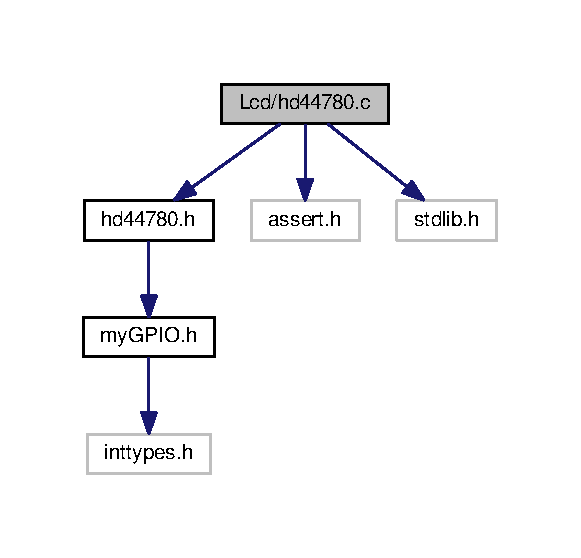
\includegraphics[width=279pt]{hd44780_8c__incl}
\end{center}
\end{figure}
\subsection*{Definizioni}
\begin{DoxyCompactItemize}
\item 
\#define \hyperlink{hd44780_8c_abc1164ac56b1a748e0ad8319be7dede8}{H\+D44780\+\_\+clear}~0x01
\item 
\#define \hyperlink{hd44780_8c_a04358db2424f9713cfb84a4fdef5b215}{H\+D44780\+\_\+home}~0x02
\item 
\#define \hyperlink{hd44780_8c_ab2681dc65568d9ec0818989aafe2eceb}{H\+D44780\+\_\+row1}~0x80
\item 
\#define \hyperlink{hd44780_8c_a7d9675a9d89c1228ada73be6239f7ef6}{H\+D44780\+\_\+row2}~0x\+C0
\item 
\#define \hyperlink{hd44780_8c_a3e52e42643f6840db3e878e23a3f82d9}{H\+D44780\+\_\+cursor\+\_\+r}~0x14
\item 
\#define \hyperlink{hd44780_8c_ad599eadde9b68b5c84f26575229383cc}{H\+D44780\+\_\+cursor\+\_\+l}~0x10
\item 
\#define \hyperlink{hd44780_8c_ab74128cead7d82100cff55cac513457a}{H\+D44780\+\_\+display\+\_\+off}~0x08
\item 
\#define \hyperlink{hd44780_8c_a05c02e143086d4d3e16c651da46357e5}{H\+D44780\+\_\+cursor\+\_\+off}~0x0\+C
\item 
\#define \hyperlink{hd44780_8c_a3967b259a0236cb4ff71b58e9e99d871}{H\+D44780\+\_\+cursor\+\_\+on}~0x0\+E
\item 
\#define \hyperlink{hd44780_8c_aee7a3931ecea03871d152b6f2fe237de}{H\+D44780\+\_\+cursor\+\_\+blink}~0x0\+F
\item 
\#define \hyperlink{hd44780_8c_abc1164ac56b1a748e0ad8319be7dede8}{H\+D44780\+\_\+clear}~0x01
\item 
\#define \hyperlink{hd44780_8c_a89582792c79342e5e196c3af6b58e813}{H\+D44780\+\_\+dec\+\_\+no\+\_\+shift}~0x04
\item 
\#define \hyperlink{hd44780_8c_a46be67bdaf1d9806e6080fc8a302e9f4}{H\+D44780\+\_\+dec\+\_\+shift}~0x05
\item 
\#define \hyperlink{hd44780_8c_a7998cf2572859cfc7a96146f9d84a8e6}{H\+D44780\+\_\+inc\+\_\+no\+\_\+shift}~0x06
\item 
\#define \hyperlink{hd44780_8c_a6c116ccd854428b9977ace77603e98f9}{H\+D44780\+\_\+inc\+\_\+shift}~0x07
\item 
\#define \hyperlink{hd44780_8c_a5f45c877d1e8266f8a2c1d0b87746950}{timer\+\_\+wait\+\_\+ms}(ms)~usleep(ms$<$$<$10)
\item 
\#define \hyperlink{hd44780_8c_a9f0a484de0de3ab1ddd77d5f716dea96}{timer\+\_\+wait\+\_\+us}(us)~usleep(us)
\item 
\#define \hyperlink{hd44780_8c_a5060e38ac985451fad57ed890aea1d77}{lcd\+\_\+command}(lcd)~\hyperlink{group__my_g_p_i_o_gab742e68093ad4c90fe299b64fd6736ca}{my\+G\+P\+I\+O\+\_\+set\+Value}(lcd-\/$>$gpio, lcd-\/$>$R\+S, \hyperlink{group__my_g_p_i_o_ggaf634fe4a0e1eab8da5000b72d6ad362ba98cde80dbda025bd1ae7231c76b55674}{my\+G\+P\+I\+O\+\_\+reset})
\item 
\#define \hyperlink{hd44780_8c_afac15d58a1ee77e8a17bc57252468ea1}{lcd\+\_\+data}(lcd)~\hyperlink{group__my_g_p_i_o_gab742e68093ad4c90fe299b64fd6736ca}{my\+G\+P\+I\+O\+\_\+set\+Value}(lcd-\/$>$gpio, lcd-\/$>$R\+S, \hyperlink{group__my_g_p_i_o_ggaf634fe4a0e1eab8da5000b72d6ad362ba10d296f3711d01189cc6c2d87f7c9149}{my\+G\+P\+I\+O\+\_\+set})
\item 
\#define \hyperlink{hd44780_8c_a7546bbb2f97e50a0469cf71934ac18e2}{lcd\+\_\+write}(lcd)~\hyperlink{group__my_g_p_i_o_gab742e68093ad4c90fe299b64fd6736ca}{my\+G\+P\+I\+O\+\_\+set\+Value}(lcd-\/$>$gpio, lcd-\/$>$R\+W, \hyperlink{group__my_g_p_i_o_ggaf634fe4a0e1eab8da5000b72d6ad362ba98cde80dbda025bd1ae7231c76b55674}{my\+G\+P\+I\+O\+\_\+reset})
\item 
\#define \hyperlink{hd44780_8c_ad7be3fdeebf9b76a774a6c1afa7fa3c8}{lcd\+\_\+read}(lcd)~\hyperlink{group__my_g_p_i_o_gab742e68093ad4c90fe299b64fd6736ca}{my\+G\+P\+I\+O\+\_\+set\+Value}(lcd-\/$>$gpio, lcd-\/$>$R\+W, \hyperlink{group__my_g_p_i_o_ggaf634fe4a0e1eab8da5000b72d6ad362ba10d296f3711d01189cc6c2d87f7c9149}{my\+G\+P\+I\+O\+\_\+set})
\item 
\#define \hyperlink{hd44780_8c_acd814f8ff18cac325b1f9f5957dd3846}{lcd\+\_\+enable}(lcd)
\end{DoxyCompactItemize}
\subsection*{Funzioni}
\begin{DoxyCompactItemize}
\item 
void \hyperlink{hd44780_8c_acc20a0564ce460f33fc998f18dd9f345}{H\+D44780\+\_\+\+Set\+Byte} (\hyperlink{struct_h_d44780___l_c_d__t}{H\+D44780\+\_\+\+L\+C\+D\+\_\+t} $\ast$lcd, uint8\+\_\+t byte)
\item 
void \hyperlink{hd44780_8c_ae12ebf4e3dd52b7d10f155e0dd1b4898}{H\+D44780\+\_\+\+Write\+Command} (\hyperlink{struct_h_d44780___l_c_d__t}{H\+D44780\+\_\+\+L\+C\+D\+\_\+t} $\ast$lcd, uint8\+\_\+t command)
\item 
void \hyperlink{hd44780_8c_a39e7e22ae76f1eec9aaf0933af398f4b}{H\+D44780\+\_\+\+Write\+Data} (\hyperlink{struct_h_d44780___l_c_d__t}{H\+D44780\+\_\+\+L\+C\+D\+\_\+t} $\ast$lcd, uint8\+\_\+t data)
\item 
int \hyperlink{hd44780_8c_ad3c60edaac713488ecb9c7ed73854a3c}{H\+D44780\+\_\+\+Validate\+Pair} (\hyperlink{struct_h_d44780___l_c_d__t}{H\+D44780\+\_\+\+L\+C\+D\+\_\+t} $\ast$lcd)
\item 
void \hyperlink{hd44780_8c_ad4120d3a2df038c193d043f386fdb221}{H\+D44780\+\_\+\+Configure\+Pin} (\hyperlink{struct_h_d44780___l_c_d__t}{H\+D44780\+\_\+\+L\+C\+D\+\_\+t} $\ast$lcd)
\item 
void \hyperlink{group___h_d44780_gad212907e20316f4fc0e93d7c7a8f338e}{H\+D44780\+\_\+\+Init8} (\hyperlink{struct_h_d44780___l_c_d__t}{H\+D44780\+\_\+\+L\+C\+D\+\_\+t} $\ast$lcd, \hyperlink{structmy_g_p_i_o__t}{my\+G\+P\+I\+O\+\_\+t} $\ast$gpio, \hyperlink{group__my_g_p_i_o_ga402a0d20afc0cb7c25554b8b023f4253}{my\+G\+P\+I\+O\+\_\+mask} R\+S, \hyperlink{group__my_g_p_i_o_ga402a0d20afc0cb7c25554b8b023f4253}{my\+G\+P\+I\+O\+\_\+mask} R\+W, \hyperlink{group__my_g_p_i_o_ga402a0d20afc0cb7c25554b8b023f4253}{my\+G\+P\+I\+O\+\_\+mask} E, \hyperlink{group__my_g_p_i_o_ga402a0d20afc0cb7c25554b8b023f4253}{my\+G\+P\+I\+O\+\_\+mask} Data7, \hyperlink{group__my_g_p_i_o_ga402a0d20afc0cb7c25554b8b023f4253}{my\+G\+P\+I\+O\+\_\+mask} Data6, \hyperlink{group__my_g_p_i_o_ga402a0d20afc0cb7c25554b8b023f4253}{my\+G\+P\+I\+O\+\_\+mask} Data5, \hyperlink{group__my_g_p_i_o_ga402a0d20afc0cb7c25554b8b023f4253}{my\+G\+P\+I\+O\+\_\+mask} Data4, \hyperlink{group__my_g_p_i_o_ga402a0d20afc0cb7c25554b8b023f4253}{my\+G\+P\+I\+O\+\_\+mask} Data3, \hyperlink{group__my_g_p_i_o_ga402a0d20afc0cb7c25554b8b023f4253}{my\+G\+P\+I\+O\+\_\+mask} Data2, \hyperlink{group__my_g_p_i_o_ga402a0d20afc0cb7c25554b8b023f4253}{my\+G\+P\+I\+O\+\_\+mask} Data1, \hyperlink{group__my_g_p_i_o_ga402a0d20afc0cb7c25554b8b023f4253}{my\+G\+P\+I\+O\+\_\+mask} Data0)
\begin{DoxyCompactList}\small\item\em Inizializza un display lcd H\+D44780 con interfacciamento ad 8 bit. \end{DoxyCompactList}\item 
void \hyperlink{group___h_d44780_ga0c08f9e41d770ebfa4af385a56b47b81}{H\+D44780\+\_\+\+Init4} (\hyperlink{struct_h_d44780___l_c_d__t}{H\+D44780\+\_\+\+L\+C\+D\+\_\+t} $\ast$lcd, \hyperlink{structmy_g_p_i_o__t}{my\+G\+P\+I\+O\+\_\+t} $\ast$gpio, \hyperlink{group__my_g_p_i_o_ga402a0d20afc0cb7c25554b8b023f4253}{my\+G\+P\+I\+O\+\_\+mask} R\+S, \hyperlink{group__my_g_p_i_o_ga402a0d20afc0cb7c25554b8b023f4253}{my\+G\+P\+I\+O\+\_\+mask} R\+W, \hyperlink{group__my_g_p_i_o_ga402a0d20afc0cb7c25554b8b023f4253}{my\+G\+P\+I\+O\+\_\+mask} E, \hyperlink{group__my_g_p_i_o_ga402a0d20afc0cb7c25554b8b023f4253}{my\+G\+P\+I\+O\+\_\+mask} Data7, \hyperlink{group__my_g_p_i_o_ga402a0d20afc0cb7c25554b8b023f4253}{my\+G\+P\+I\+O\+\_\+mask} Data6, \hyperlink{group__my_g_p_i_o_ga402a0d20afc0cb7c25554b8b023f4253}{my\+G\+P\+I\+O\+\_\+mask} Data5, \hyperlink{group__my_g_p_i_o_ga402a0d20afc0cb7c25554b8b023f4253}{my\+G\+P\+I\+O\+\_\+mask} Data4)
\begin{DoxyCompactList}\small\item\em Inizializza un oggetto display lcd H\+D44780 affinche' si utilizzi l'interfaccia a 4 bit. \end{DoxyCompactList}\item 
void \hyperlink{group___h_d44780_ga57b8c6ca0b3c12e5f7273b3c373a6f17}{H\+D44780\+\_\+\+Printc} (\hyperlink{struct_h_d44780___l_c_d__t}{H\+D44780\+\_\+\+L\+C\+D\+\_\+t} $\ast$lcd, char c)
\begin{DoxyCompactList}\small\item\em Stampa un carattere. \end{DoxyCompactList}\item 
void \hyperlink{group___h_d44780_ga3aedff8e2040e62db569fde955d3987b}{H\+D44780\+\_\+\+Print} (\hyperlink{struct_h_d44780___l_c_d__t}{H\+D44780\+\_\+\+L\+C\+D\+\_\+t} $\ast$lcd, const char $\ast$s)
\begin{DoxyCompactList}\small\item\em Stampa una stringa null-\/terminated di caratteri. \end{DoxyCompactList}\item 
void \hyperlink{group___h_d44780_ga2a5d4d528175321c46c790b581959e63}{H\+D44780\+\_\+print\+Binary8} (\hyperlink{struct_h_d44780___l_c_d__t}{H\+D44780\+\_\+\+L\+C\+D\+\_\+t} $\ast$lcd, uint8\+\_\+t b)
\begin{DoxyCompactList}\small\item\em Stampa un byte in binario. (bit piu' significativo a sinistra) \end{DoxyCompactList}\item 
void \hyperlink{group___h_d44780_ga95cceef2401c5519295e5a83c6688b5c}{H\+D44780\+\_\+print\+Binary32} (\hyperlink{struct_h_d44780___l_c_d__t}{H\+D44780\+\_\+\+L\+C\+D\+\_\+t} $\ast$lcd, uint32\+\_\+t w)
\begin{DoxyCompactList}\small\item\em Stampa una word di 32 bit in binario. (bit piu' significativo a sinistra) \end{DoxyCompactList}\item 
void \hyperlink{group___h_d44780_ga0f99bc5458acb172d0f3bfeb94f90e2a}{H\+D44780\+\_\+print\+Binary64} (\hyperlink{struct_h_d44780___l_c_d__t}{H\+D44780\+\_\+\+L\+C\+D\+\_\+t} $\ast$lcd, uint64\+\_\+t b)
\begin{DoxyCompactList}\small\item\em Stampa un blocco di 64 bit in binario. (bit piu' significativo a sinistra) \end{DoxyCompactList}\item 
void \hyperlink{group___h_d44780_gad967bd458b4d2bd358a93cbb7144addd}{H\+D44780\+\_\+print\+Hex8} (\hyperlink{struct_h_d44780___l_c_d__t}{H\+D44780\+\_\+\+L\+C\+D\+\_\+t} $\ast$lcd, uint8\+\_\+t b)
\begin{DoxyCompactList}\small\item\em Stampa un byte in esadecimale. (bit piu' significativo a sinistra) \end{DoxyCompactList}\item 
void \hyperlink{group___h_d44780_gaa82a2a27a3008f55c969a2d390c50497}{H\+D44780\+\_\+print\+Hex32} (\hyperlink{struct_h_d44780___l_c_d__t}{H\+D44780\+\_\+\+L\+C\+D\+\_\+t} $\ast$lcd, uint32\+\_\+t w)
\begin{DoxyCompactList}\small\item\em Stampa una word di 32 bit in esadecimale. (bit piu' significativo a sinistra) \end{DoxyCompactList}\item 
void \hyperlink{group___h_d44780_ga7a4b110e7da806f8c01e01d184d3a19a}{H\+D44780\+\_\+print\+Hex64} (\hyperlink{struct_h_d44780___l_c_d__t}{H\+D44780\+\_\+\+L\+C\+D\+\_\+t} $\ast$lcd, uint64\+\_\+t b)
\begin{DoxyCompactList}\small\item\em Stampa un blocco di 64 bit in esadecimale. (bit piu' significativo a sinistra) \end{DoxyCompactList}\item 
void \hyperlink{group___h_d44780_ga38cac13d7a66f068be54f79a716ff7d4}{H\+D44780\+\_\+\+Clear} (\hyperlink{struct_h_d44780___l_c_d__t}{H\+D44780\+\_\+\+L\+C\+D\+\_\+t} $\ast$lcd)
\begin{DoxyCompactList}\small\item\em Pulisce il display e sposta il cursore all'inizio della prima riga. \end{DoxyCompactList}\item 
void \hyperlink{group___h_d44780_ga68e3712332aa9482d4bdaa4991a92127}{H\+D44780\+\_\+\+Home} (\hyperlink{struct_h_d44780___l_c_d__t}{H\+D44780\+\_\+\+L\+C\+D\+\_\+t} $\ast$lcd)
\begin{DoxyCompactList}\small\item\em Sposta il cursore all'inizio della prima riga. \end{DoxyCompactList}\item 
void \hyperlink{group___h_d44780_gad90e2924a4e632ce42940323f8f49e37}{H\+D44780\+\_\+\+Move\+To\+Row1} (\hyperlink{struct_h_d44780___l_c_d__t}{H\+D44780\+\_\+\+L\+C\+D\+\_\+t} $\ast$lcd)
\begin{DoxyCompactList}\small\item\em Sposta il cursore all'inizio della prima riga. \end{DoxyCompactList}\item 
void \hyperlink{group___h_d44780_ga713670d498b6f5d50a174df19081c515}{H\+D44780\+\_\+\+Move\+To\+Row2} (\hyperlink{struct_h_d44780___l_c_d__t}{H\+D44780\+\_\+\+L\+C\+D\+\_\+t} $\ast$lcd)
\begin{DoxyCompactList}\small\item\em Sposta il cursore all'inizio della seconda riga. \end{DoxyCompactList}\item 
void \hyperlink{group___h_d44780_gabcea9a03050c46530e39b7556c673baf}{H\+D44780\+\_\+\+Move\+Cursor} (\hyperlink{struct_h_d44780___l_c_d__t}{H\+D44780\+\_\+\+L\+C\+D\+\_\+t} $\ast$lcd, \hyperlink{group___h_d44780_gaf46f4db4f981d3a1088804a6d6980d30}{H\+D44780\+\_\+\+Direction\+\_\+t} dir)
\begin{DoxyCompactList}\small\item\em Sposta il cursore di una posizione a destra o sinistra. \end{DoxyCompactList}\item 
void \hyperlink{group___h_d44780_ga5cf07b2179272029410f9a81f56621ed}{H\+D44780\+\_\+\+Display\+Off} (\hyperlink{struct_h_d44780___l_c_d__t}{H\+D44780\+\_\+\+L\+C\+D\+\_\+t} $\ast$lcd)
\begin{DoxyCompactList}\small\item\em Disattiva il display. \end{DoxyCompactList}\item 
void \hyperlink{group___h_d44780_ga56421dc398825188aa10257063a3ee4b}{H\+D44780\+\_\+\+Cursor\+Off} (\hyperlink{struct_h_d44780___l_c_d__t}{H\+D44780\+\_\+\+L\+C\+D\+\_\+t} $\ast$lcd)
\begin{DoxyCompactList}\small\item\em Disattiva la visualizzazione del cursore. \end{DoxyCompactList}\item 
void \hyperlink{group___h_d44780_ga3a381cb44df5d76d79be5ed71a52bae6}{H\+D44780\+\_\+\+Cursor\+On} (\hyperlink{struct_h_d44780___l_c_d__t}{H\+D44780\+\_\+\+L\+C\+D\+\_\+t} $\ast$lcd)
\begin{DoxyCompactList}\small\item\em Attiva la visualizzazione del cursore. \end{DoxyCompactList}\item 
void \hyperlink{group___h_d44780_ga92eb58cb7d73c9a87b7087a9c56f73d5}{H\+D44780\+\_\+\+Cursor\+Blink} (\hyperlink{struct_h_d44780___l_c_d__t}{H\+D44780\+\_\+\+L\+C\+D\+\_\+t} $\ast$lcd)
\begin{DoxyCompactList}\small\item\em Attiva il cursore lampeggiante. \end{DoxyCompactList}\end{DoxyCompactItemize}


\subsection{Descrizione dettagliata}
\begin{DoxyAuthor}{Autore}
Salvatore Barone \href{mailto:salvator.barone@gmail.com}{\tt salvator.\+barone@gmail.\+com}
\end{DoxyAuthor}
\begin{DoxyCopyright}{Copyright}
Copyright 2017 Salvatore Barone \href{mailto:salvator.barone@gmail.com}{\tt salvator.\+barone@gmail.\+com}
\end{DoxyCopyright}
This file is part of Zynq7000\+Driver\+Pack

Zynq7000\+Driver\+Pack is free software; you can redistribute it and/or modify it under the terms of the G\+N\+U General Public License as published by the Free Software Foundation; either version 3 of the License, or any later version.

Zynq7000\+Driver\+Pack is distributed in the hope that it will be useful, but W\+I\+T\+H\+O\+U\+T A\+N\+Y W\+A\+R\+R\+A\+N\+T\+Y; without even the implied warranty of M\+E\+R\+C\+H\+A\+N\+T\+A\+B\+I\+L\+I\+T\+Y or F\+I\+T\+N\+E\+S\+S F\+O\+R A P\+A\+R\+T\+I\+C\+U\+L\+A\+R P\+U\+R\+P\+O\+S\+E. See the G\+N\+U General Public License for more details.

You should have received a copy of the G\+N\+U General Public License along with this program; if not, write to the Free Software Foundation, Inc., 51 Franklin Street, Fifth Floor, Boston, M\+A 02110-\/1301, U\+S\+A. 

\subsection{Documentazione delle definizioni}
\hypertarget{hd44780_8c_abc1164ac56b1a748e0ad8319be7dede8}{\index{hd44780.\+c@{hd44780.\+c}!H\+D44780\+\_\+clear@{H\+D44780\+\_\+clear}}
\index{H\+D44780\+\_\+clear@{H\+D44780\+\_\+clear}!hd44780.\+c@{hd44780.\+c}}
\subsubsection[{H\+D44780\+\_\+clear}]{\setlength{\rightskip}{0pt plus 5cm}\#define H\+D44780\+\_\+clear~0x01}}\label{hd44780_8c_abc1164ac56b1a748e0ad8319be7dede8}
\hypertarget{hd44780_8c_abc1164ac56b1a748e0ad8319be7dede8}{\index{hd44780.\+c@{hd44780.\+c}!H\+D44780\+\_\+clear@{H\+D44780\+\_\+clear}}
\index{H\+D44780\+\_\+clear@{H\+D44780\+\_\+clear}!hd44780.\+c@{hd44780.\+c}}
\subsubsection[{H\+D44780\+\_\+clear}]{\setlength{\rightskip}{0pt plus 5cm}\#define H\+D44780\+\_\+clear~0x01}}\label{hd44780_8c_abc1164ac56b1a748e0ad8319be7dede8}
\hypertarget{hd44780_8c_aee7a3931ecea03871d152b6f2fe237de}{\index{hd44780.\+c@{hd44780.\+c}!H\+D44780\+\_\+cursor\+\_\+blink@{H\+D44780\+\_\+cursor\+\_\+blink}}
\index{H\+D44780\+\_\+cursor\+\_\+blink@{H\+D44780\+\_\+cursor\+\_\+blink}!hd44780.\+c@{hd44780.\+c}}
\subsubsection[{H\+D44780\+\_\+cursor\+\_\+blink}]{\setlength{\rightskip}{0pt plus 5cm}\#define H\+D44780\+\_\+cursor\+\_\+blink~0x0\+F}}\label{hd44780_8c_aee7a3931ecea03871d152b6f2fe237de}
\hypertarget{hd44780_8c_ad599eadde9b68b5c84f26575229383cc}{\index{hd44780.\+c@{hd44780.\+c}!H\+D44780\+\_\+cursor\+\_\+l@{H\+D44780\+\_\+cursor\+\_\+l}}
\index{H\+D44780\+\_\+cursor\+\_\+l@{H\+D44780\+\_\+cursor\+\_\+l}!hd44780.\+c@{hd44780.\+c}}
\subsubsection[{H\+D44780\+\_\+cursor\+\_\+l}]{\setlength{\rightskip}{0pt plus 5cm}\#define H\+D44780\+\_\+cursor\+\_\+l~0x10}}\label{hd44780_8c_ad599eadde9b68b5c84f26575229383cc}
\hypertarget{hd44780_8c_a05c02e143086d4d3e16c651da46357e5}{\index{hd44780.\+c@{hd44780.\+c}!H\+D44780\+\_\+cursor\+\_\+off@{H\+D44780\+\_\+cursor\+\_\+off}}
\index{H\+D44780\+\_\+cursor\+\_\+off@{H\+D44780\+\_\+cursor\+\_\+off}!hd44780.\+c@{hd44780.\+c}}
\subsubsection[{H\+D44780\+\_\+cursor\+\_\+off}]{\setlength{\rightskip}{0pt plus 5cm}\#define H\+D44780\+\_\+cursor\+\_\+off~0x0\+C}}\label{hd44780_8c_a05c02e143086d4d3e16c651da46357e5}
\hypertarget{hd44780_8c_a3967b259a0236cb4ff71b58e9e99d871}{\index{hd44780.\+c@{hd44780.\+c}!H\+D44780\+\_\+cursor\+\_\+on@{H\+D44780\+\_\+cursor\+\_\+on}}
\index{H\+D44780\+\_\+cursor\+\_\+on@{H\+D44780\+\_\+cursor\+\_\+on}!hd44780.\+c@{hd44780.\+c}}
\subsubsection[{H\+D44780\+\_\+cursor\+\_\+on}]{\setlength{\rightskip}{0pt plus 5cm}\#define H\+D44780\+\_\+cursor\+\_\+on~0x0\+E}}\label{hd44780_8c_a3967b259a0236cb4ff71b58e9e99d871}
\hypertarget{hd44780_8c_a3e52e42643f6840db3e878e23a3f82d9}{\index{hd44780.\+c@{hd44780.\+c}!H\+D44780\+\_\+cursor\+\_\+r@{H\+D44780\+\_\+cursor\+\_\+r}}
\index{H\+D44780\+\_\+cursor\+\_\+r@{H\+D44780\+\_\+cursor\+\_\+r}!hd44780.\+c@{hd44780.\+c}}
\subsubsection[{H\+D44780\+\_\+cursor\+\_\+r}]{\setlength{\rightskip}{0pt plus 5cm}\#define H\+D44780\+\_\+cursor\+\_\+r~0x14}}\label{hd44780_8c_a3e52e42643f6840db3e878e23a3f82d9}
\hypertarget{hd44780_8c_a89582792c79342e5e196c3af6b58e813}{\index{hd44780.\+c@{hd44780.\+c}!H\+D44780\+\_\+dec\+\_\+no\+\_\+shift@{H\+D44780\+\_\+dec\+\_\+no\+\_\+shift}}
\index{H\+D44780\+\_\+dec\+\_\+no\+\_\+shift@{H\+D44780\+\_\+dec\+\_\+no\+\_\+shift}!hd44780.\+c@{hd44780.\+c}}
\subsubsection[{H\+D44780\+\_\+dec\+\_\+no\+\_\+shift}]{\setlength{\rightskip}{0pt plus 5cm}\#define H\+D44780\+\_\+dec\+\_\+no\+\_\+shift~0x04}}\label{hd44780_8c_a89582792c79342e5e196c3af6b58e813}
\hypertarget{hd44780_8c_a46be67bdaf1d9806e6080fc8a302e9f4}{\index{hd44780.\+c@{hd44780.\+c}!H\+D44780\+\_\+dec\+\_\+shift@{H\+D44780\+\_\+dec\+\_\+shift}}
\index{H\+D44780\+\_\+dec\+\_\+shift@{H\+D44780\+\_\+dec\+\_\+shift}!hd44780.\+c@{hd44780.\+c}}
\subsubsection[{H\+D44780\+\_\+dec\+\_\+shift}]{\setlength{\rightskip}{0pt plus 5cm}\#define H\+D44780\+\_\+dec\+\_\+shift~0x05}}\label{hd44780_8c_a46be67bdaf1d9806e6080fc8a302e9f4}
\hypertarget{hd44780_8c_ab74128cead7d82100cff55cac513457a}{\index{hd44780.\+c@{hd44780.\+c}!H\+D44780\+\_\+display\+\_\+off@{H\+D44780\+\_\+display\+\_\+off}}
\index{H\+D44780\+\_\+display\+\_\+off@{H\+D44780\+\_\+display\+\_\+off}!hd44780.\+c@{hd44780.\+c}}
\subsubsection[{H\+D44780\+\_\+display\+\_\+off}]{\setlength{\rightskip}{0pt plus 5cm}\#define H\+D44780\+\_\+display\+\_\+off~0x08}}\label{hd44780_8c_ab74128cead7d82100cff55cac513457a}
\hypertarget{hd44780_8c_a04358db2424f9713cfb84a4fdef5b215}{\index{hd44780.\+c@{hd44780.\+c}!H\+D44780\+\_\+home@{H\+D44780\+\_\+home}}
\index{H\+D44780\+\_\+home@{H\+D44780\+\_\+home}!hd44780.\+c@{hd44780.\+c}}
\subsubsection[{H\+D44780\+\_\+home}]{\setlength{\rightskip}{0pt plus 5cm}\#define H\+D44780\+\_\+home~0x02}}\label{hd44780_8c_a04358db2424f9713cfb84a4fdef5b215}
\hypertarget{hd44780_8c_a7998cf2572859cfc7a96146f9d84a8e6}{\index{hd44780.\+c@{hd44780.\+c}!H\+D44780\+\_\+inc\+\_\+no\+\_\+shift@{H\+D44780\+\_\+inc\+\_\+no\+\_\+shift}}
\index{H\+D44780\+\_\+inc\+\_\+no\+\_\+shift@{H\+D44780\+\_\+inc\+\_\+no\+\_\+shift}!hd44780.\+c@{hd44780.\+c}}
\subsubsection[{H\+D44780\+\_\+inc\+\_\+no\+\_\+shift}]{\setlength{\rightskip}{0pt plus 5cm}\#define H\+D44780\+\_\+inc\+\_\+no\+\_\+shift~0x06}}\label{hd44780_8c_a7998cf2572859cfc7a96146f9d84a8e6}
\hypertarget{hd44780_8c_a6c116ccd854428b9977ace77603e98f9}{\index{hd44780.\+c@{hd44780.\+c}!H\+D44780\+\_\+inc\+\_\+shift@{H\+D44780\+\_\+inc\+\_\+shift}}
\index{H\+D44780\+\_\+inc\+\_\+shift@{H\+D44780\+\_\+inc\+\_\+shift}!hd44780.\+c@{hd44780.\+c}}
\subsubsection[{H\+D44780\+\_\+inc\+\_\+shift}]{\setlength{\rightskip}{0pt plus 5cm}\#define H\+D44780\+\_\+inc\+\_\+shift~0x07}}\label{hd44780_8c_a6c116ccd854428b9977ace77603e98f9}
\hypertarget{hd44780_8c_ab2681dc65568d9ec0818989aafe2eceb}{\index{hd44780.\+c@{hd44780.\+c}!H\+D44780\+\_\+row1@{H\+D44780\+\_\+row1}}
\index{H\+D44780\+\_\+row1@{H\+D44780\+\_\+row1}!hd44780.\+c@{hd44780.\+c}}
\subsubsection[{H\+D44780\+\_\+row1}]{\setlength{\rightskip}{0pt plus 5cm}\#define H\+D44780\+\_\+row1~0x80}}\label{hd44780_8c_ab2681dc65568d9ec0818989aafe2eceb}
\hypertarget{hd44780_8c_a7d9675a9d89c1228ada73be6239f7ef6}{\index{hd44780.\+c@{hd44780.\+c}!H\+D44780\+\_\+row2@{H\+D44780\+\_\+row2}}
\index{H\+D44780\+\_\+row2@{H\+D44780\+\_\+row2}!hd44780.\+c@{hd44780.\+c}}
\subsubsection[{H\+D44780\+\_\+row2}]{\setlength{\rightskip}{0pt plus 5cm}\#define H\+D44780\+\_\+row2~0x\+C0}}\label{hd44780_8c_a7d9675a9d89c1228ada73be6239f7ef6}
\hypertarget{hd44780_8c_a5060e38ac985451fad57ed890aea1d77}{\index{hd44780.\+c@{hd44780.\+c}!lcd\+\_\+command@{lcd\+\_\+command}}
\index{lcd\+\_\+command@{lcd\+\_\+command}!hd44780.\+c@{hd44780.\+c}}
\subsubsection[{lcd\+\_\+command}]{\setlength{\rightskip}{0pt plus 5cm}\#define lcd\+\_\+command(
\begin{DoxyParamCaption}
\item[{}]{lcd}
\end{DoxyParamCaption}
)~{\bf my\+G\+P\+I\+O\+\_\+set\+Value}(lcd-\/$>$gpio, lcd-\/$>$R\+S, {\bf my\+G\+P\+I\+O\+\_\+reset})}}\label{hd44780_8c_a5060e38ac985451fad57ed890aea1d77}
\hypertarget{hd44780_8c_afac15d58a1ee77e8a17bc57252468ea1}{\index{hd44780.\+c@{hd44780.\+c}!lcd\+\_\+data@{lcd\+\_\+data}}
\index{lcd\+\_\+data@{lcd\+\_\+data}!hd44780.\+c@{hd44780.\+c}}
\subsubsection[{lcd\+\_\+data}]{\setlength{\rightskip}{0pt plus 5cm}\#define lcd\+\_\+data(
\begin{DoxyParamCaption}
\item[{}]{lcd}
\end{DoxyParamCaption}
)~{\bf my\+G\+P\+I\+O\+\_\+set\+Value}(lcd-\/$>$gpio, lcd-\/$>$R\+S, {\bf my\+G\+P\+I\+O\+\_\+set})}}\label{hd44780_8c_afac15d58a1ee77e8a17bc57252468ea1}
\hypertarget{hd44780_8c_acd814f8ff18cac325b1f9f5957dd3846}{\index{hd44780.\+c@{hd44780.\+c}!lcd\+\_\+enable@{lcd\+\_\+enable}}
\index{lcd\+\_\+enable@{lcd\+\_\+enable}!hd44780.\+c@{hd44780.\+c}}
\subsubsection[{lcd\+\_\+enable}]{\setlength{\rightskip}{0pt plus 5cm}\#define lcd\+\_\+enable(
\begin{DoxyParamCaption}
\item[{}]{lcd}
\end{DoxyParamCaption}
)}}\label{hd44780_8c_acd814f8ff18cac325b1f9f5957dd3846}
{\bfseries Valore\+:}
\begin{DoxyCode}
\hyperlink{group__my_g_p_i_o_gab742e68093ad4c90fe299b64fd6736ca}{myGPIO\_setValue}(lcd->gpio, lcd->E, \hyperlink{group__my_g_p_i_o_ggaf634fe4a0e1eab8da5000b72d6ad362ba10d296f3711d01189cc6c2d87f7c9149}{myGPIO\_set}); \hyperlink{hd44780_8c_a9f0a484de0de3ab1ddd77d5f716dea96}{\(\backslash\)}
\hyperlink{hd44780_8c_a9f0a484de0de3ab1ddd77d5f716dea96}{                            timer\_wait\_us}(100); \hyperlink{group__my_g_p_i_o_gab742e68093ad4c90fe299b64fd6736ca}{\(\backslash\)}
\hyperlink{group__my_g_p_i_o_gab742e68093ad4c90fe299b64fd6736ca}{                            myGPIO\_setValue}(lcd->gpio, lcd->E, 
      \hyperlink{group__my_g_p_i_o_ggaf634fe4a0e1eab8da5000b72d6ad362ba98cde80dbda025bd1ae7231c76b55674}{myGPIO\_reset})
\end{DoxyCode}
\hypertarget{hd44780_8c_ad7be3fdeebf9b76a774a6c1afa7fa3c8}{\index{hd44780.\+c@{hd44780.\+c}!lcd\+\_\+read@{lcd\+\_\+read}}
\index{lcd\+\_\+read@{lcd\+\_\+read}!hd44780.\+c@{hd44780.\+c}}
\subsubsection[{lcd\+\_\+read}]{\setlength{\rightskip}{0pt plus 5cm}\#define lcd\+\_\+read(
\begin{DoxyParamCaption}
\item[{}]{lcd}
\end{DoxyParamCaption}
)~{\bf my\+G\+P\+I\+O\+\_\+set\+Value}(lcd-\/$>$gpio, lcd-\/$>$R\+W, {\bf my\+G\+P\+I\+O\+\_\+set})}}\label{hd44780_8c_ad7be3fdeebf9b76a774a6c1afa7fa3c8}
\hypertarget{hd44780_8c_a7546bbb2f97e50a0469cf71934ac18e2}{\index{hd44780.\+c@{hd44780.\+c}!lcd\+\_\+write@{lcd\+\_\+write}}
\index{lcd\+\_\+write@{lcd\+\_\+write}!hd44780.\+c@{hd44780.\+c}}
\subsubsection[{lcd\+\_\+write}]{\setlength{\rightskip}{0pt plus 5cm}\#define lcd\+\_\+write(
\begin{DoxyParamCaption}
\item[{}]{lcd}
\end{DoxyParamCaption}
)~{\bf my\+G\+P\+I\+O\+\_\+set\+Value}(lcd-\/$>$gpio, lcd-\/$>$R\+W, {\bf my\+G\+P\+I\+O\+\_\+reset})}}\label{hd44780_8c_a7546bbb2f97e50a0469cf71934ac18e2}
\hypertarget{hd44780_8c_a5f45c877d1e8266f8a2c1d0b87746950}{\index{hd44780.\+c@{hd44780.\+c}!timer\+\_\+wait\+\_\+ms@{timer\+\_\+wait\+\_\+ms}}
\index{timer\+\_\+wait\+\_\+ms@{timer\+\_\+wait\+\_\+ms}!hd44780.\+c@{hd44780.\+c}}
\subsubsection[{timer\+\_\+wait\+\_\+ms}]{\setlength{\rightskip}{0pt plus 5cm}\#define timer\+\_\+wait\+\_\+ms(
\begin{DoxyParamCaption}
\item[{}]{ms}
\end{DoxyParamCaption}
)~usleep(ms$<$$<$10)}}\label{hd44780_8c_a5f45c877d1e8266f8a2c1d0b87746950}
\hypertarget{hd44780_8c_a9f0a484de0de3ab1ddd77d5f716dea96}{\index{hd44780.\+c@{hd44780.\+c}!timer\+\_\+wait\+\_\+us@{timer\+\_\+wait\+\_\+us}}
\index{timer\+\_\+wait\+\_\+us@{timer\+\_\+wait\+\_\+us}!hd44780.\+c@{hd44780.\+c}}
\subsubsection[{timer\+\_\+wait\+\_\+us}]{\setlength{\rightskip}{0pt plus 5cm}\#define timer\+\_\+wait\+\_\+us(
\begin{DoxyParamCaption}
\item[{}]{us}
\end{DoxyParamCaption}
)~usleep(us)}}\label{hd44780_8c_a9f0a484de0de3ab1ddd77d5f716dea96}


\subsection{Documentazione delle funzioni}
\hypertarget{hd44780_8c_ad4120d3a2df038c193d043f386fdb221}{\index{hd44780.\+c@{hd44780.\+c}!H\+D44780\+\_\+\+Configure\+Pin@{H\+D44780\+\_\+\+Configure\+Pin}}
\index{H\+D44780\+\_\+\+Configure\+Pin@{H\+D44780\+\_\+\+Configure\+Pin}!hd44780.\+c@{hd44780.\+c}}
\subsubsection[{H\+D44780\+\_\+\+Configure\+Pin}]{\setlength{\rightskip}{0pt plus 5cm}void H\+D44780\+\_\+\+Configure\+Pin (
\begin{DoxyParamCaption}
\item[{{\bf H\+D44780\+\_\+\+L\+C\+D\+\_\+t} $\ast$}]{lcd}
\end{DoxyParamCaption}
)}}\label{hd44780_8c_ad4120d3a2df038c193d043f386fdb221}
\hypertarget{hd44780_8c_acc20a0564ce460f33fc998f18dd9f345}{\index{hd44780.\+c@{hd44780.\+c}!H\+D44780\+\_\+\+Set\+Byte@{H\+D44780\+\_\+\+Set\+Byte}}
\index{H\+D44780\+\_\+\+Set\+Byte@{H\+D44780\+\_\+\+Set\+Byte}!hd44780.\+c@{hd44780.\+c}}
\subsubsection[{H\+D44780\+\_\+\+Set\+Byte}]{\setlength{\rightskip}{0pt plus 5cm}void H\+D44780\+\_\+\+Set\+Byte (
\begin{DoxyParamCaption}
\item[{{\bf H\+D44780\+\_\+\+L\+C\+D\+\_\+t} $\ast$}]{lcd, }
\item[{uint8\+\_\+t}]{byte}
\end{DoxyParamCaption}
)}}\label{hd44780_8c_acc20a0564ce460f33fc998f18dd9f345}
\hypertarget{hd44780_8c_ad3c60edaac713488ecb9c7ed73854a3c}{\index{hd44780.\+c@{hd44780.\+c}!H\+D44780\+\_\+\+Validate\+Pair@{H\+D44780\+\_\+\+Validate\+Pair}}
\index{H\+D44780\+\_\+\+Validate\+Pair@{H\+D44780\+\_\+\+Validate\+Pair}!hd44780.\+c@{hd44780.\+c}}
\subsubsection[{H\+D44780\+\_\+\+Validate\+Pair}]{\setlength{\rightskip}{0pt plus 5cm}int H\+D44780\+\_\+\+Validate\+Pair (
\begin{DoxyParamCaption}
\item[{{\bf H\+D44780\+\_\+\+L\+C\+D\+\_\+t} $\ast$}]{lcd}
\end{DoxyParamCaption}
)}}\label{hd44780_8c_ad3c60edaac713488ecb9c7ed73854a3c}
\hypertarget{hd44780_8c_ae12ebf4e3dd52b7d10f155e0dd1b4898}{\index{hd44780.\+c@{hd44780.\+c}!H\+D44780\+\_\+\+Write\+Command@{H\+D44780\+\_\+\+Write\+Command}}
\index{H\+D44780\+\_\+\+Write\+Command@{H\+D44780\+\_\+\+Write\+Command}!hd44780.\+c@{hd44780.\+c}}
\subsubsection[{H\+D44780\+\_\+\+Write\+Command}]{\setlength{\rightskip}{0pt plus 5cm}void H\+D44780\+\_\+\+Write\+Command (
\begin{DoxyParamCaption}
\item[{{\bf H\+D44780\+\_\+\+L\+C\+D\+\_\+t} $\ast$}]{lcd, }
\item[{uint8\+\_\+t}]{command}
\end{DoxyParamCaption}
)}}\label{hd44780_8c_ae12ebf4e3dd52b7d10f155e0dd1b4898}
\hypertarget{hd44780_8c_a39e7e22ae76f1eec9aaf0933af398f4b}{\index{hd44780.\+c@{hd44780.\+c}!H\+D44780\+\_\+\+Write\+Data@{H\+D44780\+\_\+\+Write\+Data}}
\index{H\+D44780\+\_\+\+Write\+Data@{H\+D44780\+\_\+\+Write\+Data}!hd44780.\+c@{hd44780.\+c}}
\subsubsection[{H\+D44780\+\_\+\+Write\+Data}]{\setlength{\rightskip}{0pt plus 5cm}void H\+D44780\+\_\+\+Write\+Data (
\begin{DoxyParamCaption}
\item[{{\bf H\+D44780\+\_\+\+L\+C\+D\+\_\+t} $\ast$}]{lcd, }
\item[{uint8\+\_\+t}]{data}
\end{DoxyParamCaption}
)}}\label{hd44780_8c_a39e7e22ae76f1eec9aaf0933af398f4b}

\hypertarget{hd44780_8h}{\section{Riferimenti per il file Lcd/hd44780.h}
\label{hd44780_8h}\index{Lcd/hd44780.\+h@{Lcd/hd44780.\+h}}
}
{\ttfamily \#include \char`\"{}my\+G\+P\+I\+O.\+h\char`\"{}}\\*
Grafo delle dipendenze di inclusione per hd44780.\+h\+:
\nopagebreak
\begin{figure}[H]
\begin{center}
\leavevmode
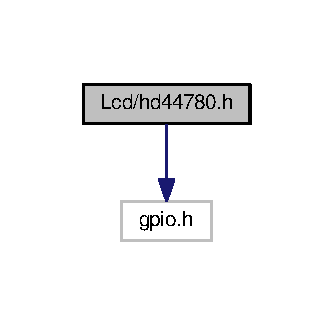
\includegraphics[width=160pt]{hd44780_8h__incl}
\end{center}
\end{figure}
Questo grafo mostra quali altri file includono direttamente o indirettamente questo file\+:\nopagebreak
\begin{figure}[H]
\begin{center}
\leavevmode
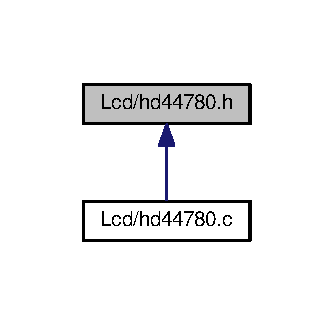
\includegraphics[width=160pt]{hd44780_8h__dep__incl}
\end{center}
\end{figure}
\subsection*{Strutture dati}
\begin{DoxyCompactItemize}
\item 
struct \hyperlink{struct_h_d44780___l_c_d__t}{H\+D44780\+\_\+\+L\+C\+D\+\_\+t}
\begin{DoxyCompactList}\small\item\em Struttura opaca che astrae un device Display L\+C\+D con cntroller Hitachi H\+D44780, o compatibile. Un oggetto di tipo \hyperlink{struct_h_d44780___l_c_d__t}{H\+D44780\+\_\+\+L\+C\+D\+\_\+t} rappresenta un device lcd H\+D44780. Il modulo e' pensato per permettere la gestione di piu' display da parte dello stesso processore, agendo su oggetti \hyperlink{struct_h_d44780___l_c_d__t}{H\+D44780\+\_\+\+L\+C\+D\+\_\+t} diversi. Il modulo permette di utilizzare sia l'interfacciamento ad otto bit che quello a quattro bit, inizializzando il device opportunamente, attraverso l'uso delle funzioni H\+D44780\+\_\+\+Init8 e\+H\+D44780\+\_\+\+Init4. Il modulo fornisce anche semplici funzioni per la stampa di un carattere o di una stringa null-\/terminated di caratteri. Si veda la documentazione delle funzioni H\+D44780\+\_\+\+Printc e H\+D44780\+\_\+\+Print. Inoltre sono presenti diverse funzioni di utilita' generica, come quelle per la pulizia del display, per lo spostamento del cursore di un posto in avanti o indietro, alla riga in basso o in alto. \end{DoxyCompactList}\end{DoxyCompactItemize}
\subsection*{Tipi enumerati (enum)}
\begin{DoxyCompactItemize}
\item 
enum \hyperlink{group___h_d44780_gaaaea8b73e24f7658da4118f6b01b45f0}{H\+D44780\+\_\+\+Interface\+Mode\+\_\+t} \{ \hyperlink{group___h_d44780_ggaaaea8b73e24f7658da4118f6b01b45f0a45bf6ce7ec7c951f692bdce9f0f485c6}{H\+D44780\+\_\+\+I\+N\+T\+E\+R\+F\+A\+C\+E\+\_\+4bit}, 
\hyperlink{group___h_d44780_ggaaaea8b73e24f7658da4118f6b01b45f0a24da9b234f9358c14184fe21f3c47de5}{H\+D44780\+\_\+\+I\+N\+T\+E\+R\+F\+A\+C\+E\+\_\+8bit}
 \}
\begin{DoxyCompactList}\small\item\em Modalita' di interfacciamento. Il modulo supporta sia interfacciamento a 4 bit che ad 8 bit. \end{DoxyCompactList}\item 
enum \hyperlink{group___h_d44780_gaf46f4db4f981d3a1088804a6d6980d30}{H\+D44780\+\_\+\+Direction\+\_\+t} \{ \hyperlink{group___h_d44780_ggaf46f4db4f981d3a1088804a6d6980d30aa4d704398d4edd1e0dec8dbb55f90292}{H\+D44780\+\_\+\+Cursor\+Left}, 
\hyperlink{group___h_d44780_ggaf46f4db4f981d3a1088804a6d6980d30a26006ced693b6bab28c6e30bfdb8c399}{H\+D44780\+\_\+\+Cursor\+Right}
 \}
\begin{DoxyCompactList}\small\item\em Direzioni di spostamento del cursore, usata dalla funzione \hyperlink{group___h_d44780_gabcea9a03050c46530e39b7556c673baf}{H\+D44780\+\_\+\+Move\+Cursor()} \end{DoxyCompactList}\end{DoxyCompactItemize}
\subsection*{Funzioni}
\begin{DoxyCompactItemize}
\item 
void \hyperlink{group___h_d44780_gad212907e20316f4fc0e93d7c7a8f338e}{H\+D44780\+\_\+\+Init8} (\hyperlink{struct_h_d44780___l_c_d__t}{H\+D44780\+\_\+\+L\+C\+D\+\_\+t} $\ast$lcd, \hyperlink{structmy_g_p_i_o__t}{my\+G\+P\+I\+O\+\_\+t} $\ast$gpio, \hyperlink{group__my_g_p_i_o_ga402a0d20afc0cb7c25554b8b023f4253}{my\+G\+P\+I\+O\+\_\+mask} R\+S, \hyperlink{group__my_g_p_i_o_ga402a0d20afc0cb7c25554b8b023f4253}{my\+G\+P\+I\+O\+\_\+mask} R\+W, \hyperlink{group__my_g_p_i_o_ga402a0d20afc0cb7c25554b8b023f4253}{my\+G\+P\+I\+O\+\_\+mask} E, \hyperlink{group__my_g_p_i_o_ga402a0d20afc0cb7c25554b8b023f4253}{my\+G\+P\+I\+O\+\_\+mask} Data7, \hyperlink{group__my_g_p_i_o_ga402a0d20afc0cb7c25554b8b023f4253}{my\+G\+P\+I\+O\+\_\+mask} Data6, \hyperlink{group__my_g_p_i_o_ga402a0d20afc0cb7c25554b8b023f4253}{my\+G\+P\+I\+O\+\_\+mask} Data5, \hyperlink{group__my_g_p_i_o_ga402a0d20afc0cb7c25554b8b023f4253}{my\+G\+P\+I\+O\+\_\+mask} Data4, \hyperlink{group__my_g_p_i_o_ga402a0d20afc0cb7c25554b8b023f4253}{my\+G\+P\+I\+O\+\_\+mask} Data3, \hyperlink{group__my_g_p_i_o_ga402a0d20afc0cb7c25554b8b023f4253}{my\+G\+P\+I\+O\+\_\+mask} Data2, \hyperlink{group__my_g_p_i_o_ga402a0d20afc0cb7c25554b8b023f4253}{my\+G\+P\+I\+O\+\_\+mask} Data1, \hyperlink{group__my_g_p_i_o_ga402a0d20afc0cb7c25554b8b023f4253}{my\+G\+P\+I\+O\+\_\+mask} Data0)
\begin{DoxyCompactList}\small\item\em Inizializza un display lcd H\+D44780 con interfacciamento ad 8 bit. \end{DoxyCompactList}\item 
void \hyperlink{group___h_d44780_ga0c08f9e41d770ebfa4af385a56b47b81}{H\+D44780\+\_\+\+Init4} (\hyperlink{struct_h_d44780___l_c_d__t}{H\+D44780\+\_\+\+L\+C\+D\+\_\+t} $\ast$lcd, \hyperlink{structmy_g_p_i_o__t}{my\+G\+P\+I\+O\+\_\+t} $\ast$gpio, \hyperlink{group__my_g_p_i_o_ga402a0d20afc0cb7c25554b8b023f4253}{my\+G\+P\+I\+O\+\_\+mask} R\+S, \hyperlink{group__my_g_p_i_o_ga402a0d20afc0cb7c25554b8b023f4253}{my\+G\+P\+I\+O\+\_\+mask} R\+W, \hyperlink{group__my_g_p_i_o_ga402a0d20afc0cb7c25554b8b023f4253}{my\+G\+P\+I\+O\+\_\+mask} E, \hyperlink{group__my_g_p_i_o_ga402a0d20afc0cb7c25554b8b023f4253}{my\+G\+P\+I\+O\+\_\+mask} Data7, \hyperlink{group__my_g_p_i_o_ga402a0d20afc0cb7c25554b8b023f4253}{my\+G\+P\+I\+O\+\_\+mask} Data6, \hyperlink{group__my_g_p_i_o_ga402a0d20afc0cb7c25554b8b023f4253}{my\+G\+P\+I\+O\+\_\+mask} Data5, \hyperlink{group__my_g_p_i_o_ga402a0d20afc0cb7c25554b8b023f4253}{my\+G\+P\+I\+O\+\_\+mask} Data4)
\begin{DoxyCompactList}\small\item\em Inizializza un oggetto display lcd H\+D44780 affinche' si utilizzi l'interfaccia a 4 bit. \end{DoxyCompactList}\item 
void \hyperlink{group___h_d44780_ga57b8c6ca0b3c12e5f7273b3c373a6f17}{H\+D44780\+\_\+\+Printc} (\hyperlink{struct_h_d44780___l_c_d__t}{H\+D44780\+\_\+\+L\+C\+D\+\_\+t} $\ast$lcd, char c)
\begin{DoxyCompactList}\small\item\em Stampa un carattere. \end{DoxyCompactList}\item 
void \hyperlink{group___h_d44780_ga3aedff8e2040e62db569fde955d3987b}{H\+D44780\+\_\+\+Print} (\hyperlink{struct_h_d44780___l_c_d__t}{H\+D44780\+\_\+\+L\+C\+D\+\_\+t} $\ast$lcd, const char $\ast$s)
\begin{DoxyCompactList}\small\item\em Stampa una stringa null-\/terminated di caratteri. \end{DoxyCompactList}\item 
void \hyperlink{group___h_d44780_ga2a5d4d528175321c46c790b581959e63}{H\+D44780\+\_\+print\+Binary8} (\hyperlink{struct_h_d44780___l_c_d__t}{H\+D44780\+\_\+\+L\+C\+D\+\_\+t} $\ast$lcd, uint8\+\_\+t b)
\begin{DoxyCompactList}\small\item\em Stampa un byte in binario. (bit piu' significativo a sinistra) \end{DoxyCompactList}\item 
void \hyperlink{group___h_d44780_ga95cceef2401c5519295e5a83c6688b5c}{H\+D44780\+\_\+print\+Binary32} (\hyperlink{struct_h_d44780___l_c_d__t}{H\+D44780\+\_\+\+L\+C\+D\+\_\+t} $\ast$lcd, uint32\+\_\+t w)
\begin{DoxyCompactList}\small\item\em Stampa una word di 32 bit in binario. (bit piu' significativo a sinistra) \end{DoxyCompactList}\item 
void \hyperlink{group___h_d44780_ga0f99bc5458acb172d0f3bfeb94f90e2a}{H\+D44780\+\_\+print\+Binary64} (\hyperlink{struct_h_d44780___l_c_d__t}{H\+D44780\+\_\+\+L\+C\+D\+\_\+t} $\ast$lcd, uint64\+\_\+t b)
\begin{DoxyCompactList}\small\item\em Stampa un blocco di 64 bit in binario. (bit piu' significativo a sinistra) \end{DoxyCompactList}\item 
void \hyperlink{group___h_d44780_gad967bd458b4d2bd358a93cbb7144addd}{H\+D44780\+\_\+print\+Hex8} (\hyperlink{struct_h_d44780___l_c_d__t}{H\+D44780\+\_\+\+L\+C\+D\+\_\+t} $\ast$lcd, uint8\+\_\+t b)
\begin{DoxyCompactList}\small\item\em Stampa un byte in esadecimale. (bit piu' significativo a sinistra) \end{DoxyCompactList}\item 
void \hyperlink{group___h_d44780_gaa82a2a27a3008f55c969a2d390c50497}{H\+D44780\+\_\+print\+Hex32} (\hyperlink{struct_h_d44780___l_c_d__t}{H\+D44780\+\_\+\+L\+C\+D\+\_\+t} $\ast$lcd, uint32\+\_\+t w)
\begin{DoxyCompactList}\small\item\em Stampa una word di 32 bit in esadecimale. (bit piu' significativo a sinistra) \end{DoxyCompactList}\item 
void \hyperlink{group___h_d44780_ga7a4b110e7da806f8c01e01d184d3a19a}{H\+D44780\+\_\+print\+Hex64} (\hyperlink{struct_h_d44780___l_c_d__t}{H\+D44780\+\_\+\+L\+C\+D\+\_\+t} $\ast$lcd, uint64\+\_\+t b)
\begin{DoxyCompactList}\small\item\em Stampa un blocco di 64 bit in esadecimale. (bit piu' significativo a sinistra) \end{DoxyCompactList}\item 
void \hyperlink{group___h_d44780_ga38cac13d7a66f068be54f79a716ff7d4}{H\+D44780\+\_\+\+Clear} (\hyperlink{struct_h_d44780___l_c_d__t}{H\+D44780\+\_\+\+L\+C\+D\+\_\+t} $\ast$lcd)
\begin{DoxyCompactList}\small\item\em Pulisce il display e sposta il cursore all'inizio della prima riga. \end{DoxyCompactList}\item 
void \hyperlink{group___h_d44780_ga68e3712332aa9482d4bdaa4991a92127}{H\+D44780\+\_\+\+Home} (\hyperlink{struct_h_d44780___l_c_d__t}{H\+D44780\+\_\+\+L\+C\+D\+\_\+t} $\ast$lcd)
\begin{DoxyCompactList}\small\item\em Sposta il cursore all'inizio della prima riga. \end{DoxyCompactList}\item 
void \hyperlink{group___h_d44780_gad90e2924a4e632ce42940323f8f49e37}{H\+D44780\+\_\+\+Move\+To\+Row1} (\hyperlink{struct_h_d44780___l_c_d__t}{H\+D44780\+\_\+\+L\+C\+D\+\_\+t} $\ast$lcd)
\begin{DoxyCompactList}\small\item\em Sposta il cursore all'inizio della prima riga. \end{DoxyCompactList}\item 
void \hyperlink{group___h_d44780_ga713670d498b6f5d50a174df19081c515}{H\+D44780\+\_\+\+Move\+To\+Row2} (\hyperlink{struct_h_d44780___l_c_d__t}{H\+D44780\+\_\+\+L\+C\+D\+\_\+t} $\ast$lcd)
\begin{DoxyCompactList}\small\item\em Sposta il cursore all'inizio della seconda riga. \end{DoxyCompactList}\item 
void \hyperlink{group___h_d44780_gabcea9a03050c46530e39b7556c673baf}{H\+D44780\+\_\+\+Move\+Cursor} (\hyperlink{struct_h_d44780___l_c_d__t}{H\+D44780\+\_\+\+L\+C\+D\+\_\+t} $\ast$lcd, \hyperlink{group___h_d44780_gaf46f4db4f981d3a1088804a6d6980d30}{H\+D44780\+\_\+\+Direction\+\_\+t} dir)
\begin{DoxyCompactList}\small\item\em Sposta il cursore di una posizione a destra o sinistra. \end{DoxyCompactList}\item 
void \hyperlink{group___h_d44780_ga5cf07b2179272029410f9a81f56621ed}{H\+D44780\+\_\+\+Display\+Off} (\hyperlink{struct_h_d44780___l_c_d__t}{H\+D44780\+\_\+\+L\+C\+D\+\_\+t} $\ast$lcd)
\begin{DoxyCompactList}\small\item\em Disattiva il display. \end{DoxyCompactList}\item 
void \hyperlink{group___h_d44780_ga56421dc398825188aa10257063a3ee4b}{H\+D44780\+\_\+\+Cursor\+Off} (\hyperlink{struct_h_d44780___l_c_d__t}{H\+D44780\+\_\+\+L\+C\+D\+\_\+t} $\ast$lcd)
\begin{DoxyCompactList}\small\item\em Disattiva la visualizzazione del cursore. \end{DoxyCompactList}\item 
void \hyperlink{group___h_d44780_ga3a381cb44df5d76d79be5ed71a52bae6}{H\+D44780\+\_\+\+Cursor\+On} (\hyperlink{struct_h_d44780___l_c_d__t}{H\+D44780\+\_\+\+L\+C\+D\+\_\+t} $\ast$lcd)
\begin{DoxyCompactList}\small\item\em Attiva la visualizzazione del cursore. \end{DoxyCompactList}\item 
void \hyperlink{group___h_d44780_ga92eb58cb7d73c9a87b7087a9c56f73d5}{H\+D44780\+\_\+\+Cursor\+Blink} (\hyperlink{struct_h_d44780___l_c_d__t}{H\+D44780\+\_\+\+L\+C\+D\+\_\+t} $\ast$lcd)
\begin{DoxyCompactList}\small\item\em Attiva il cursore lampeggiante. \end{DoxyCompactList}\end{DoxyCompactItemize}

\hypertarget{_zybo_8h}{}\section{Riferimenti per il file Src/my\+G\+P\+I\+O/bare-\/metal/\+Zybo\+B\+S\+P/\+Zybo.h}
\label{_zybo_8h}\index{Src/my\+G\+P\+I\+O/bare-\/metal/\+Zybo\+B\+S\+P/\+Zybo.\+h@{Src/my\+G\+P\+I\+O/bare-\/metal/\+Zybo\+B\+S\+P/\+Zybo.\+h}}
{\ttfamily \#include \char`\"{}Zybo\+Led.\+h\char`\"{}}\newline
{\ttfamily \#include \char`\"{}Zybo\+Switch.\+h\char`\"{}}\newline
{\ttfamily \#include \char`\"{}Zybo\+Button.\+h\char`\"{}}\newline
Grafo delle dipendenze di inclusione per Zybo.\+h\+:\nopagebreak
\begin{figure}[H]
\begin{center}
\leavevmode
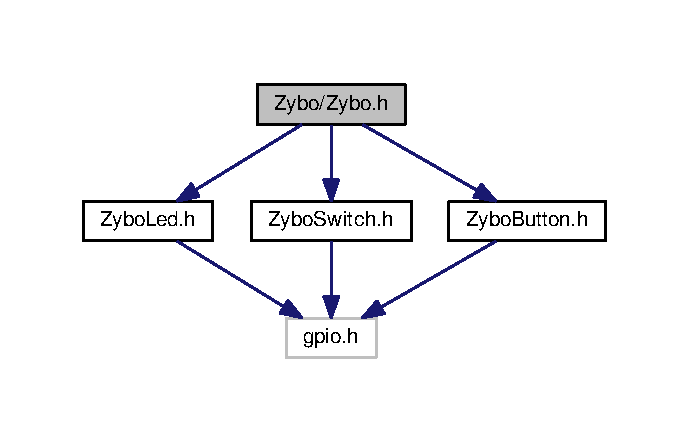
\includegraphics[width=331pt]{_zybo_8h__incl}
\end{center}
\end{figure}


\subsection{Descrizione dettagliata}
\begin{DoxyAuthor}{Autore}
Salvatore Barone \href{mailto:salvator.barone@gmail.com}{\tt salvator.\+barone@gmail.\+com}
\end{DoxyAuthor}
\begin{DoxyCopyright}{Copyright}
Copyright 2017 Salvatore Barone \href{mailto:salvator.barone@gmail.com}{\tt salvator.\+barone@gmail.\+com}
\end{DoxyCopyright}
This file is part of Zynq7000\+Driver\+Pack

Zynq7000\+Driver\+Pack is free software; you can redistribute it and/or modify it under the terms of the G\+NU General Public License as published by the Free Software Foundation; either version 3 of the License, or any later version.

Zynq7000\+Driver\+Pack is distributed in the hope that it will be useful, but W\+I\+T\+H\+O\+UT A\+NY W\+A\+R\+R\+A\+N\+TY; without even the implied warranty of M\+E\+R\+C\+H\+A\+N\+T\+A\+B\+I\+L\+I\+TY or F\+I\+T\+N\+E\+SS F\+OR A P\+A\+R\+T\+I\+C\+U\+L\+AR P\+U\+R\+P\+O\+SE. See the G\+NU General Public License for more details.

You should have received a copy of the G\+NU General Public License along with this program; if not, write to the Free Software Foundation, Inc., 51 Franklin Street, Fifth Floor, Boston, MA 02110-\/1301, U\+SA. 
\hypertarget{_zybo_button_8c}{\section{Riferimenti per il file Zybo/\+Zybo\+Button.c}
\label{_zybo_button_8c}\index{Zybo/\+Zybo\+Button.\+c@{Zybo/\+Zybo\+Button.\+c}}
}
{\ttfamily \#include \char`\"{}Zybo\+Button.\+h\char`\"{}}\\*
{\ttfamily \#include $<$assert.\+h$>$}\\*
{\ttfamily \#include $<$stdlib.\+h$>$}\\*
Grafo delle dipendenze di inclusione per Zybo\+Button.\+c\+:
\nopagebreak
\begin{figure}[H]
\begin{center}
\leavevmode
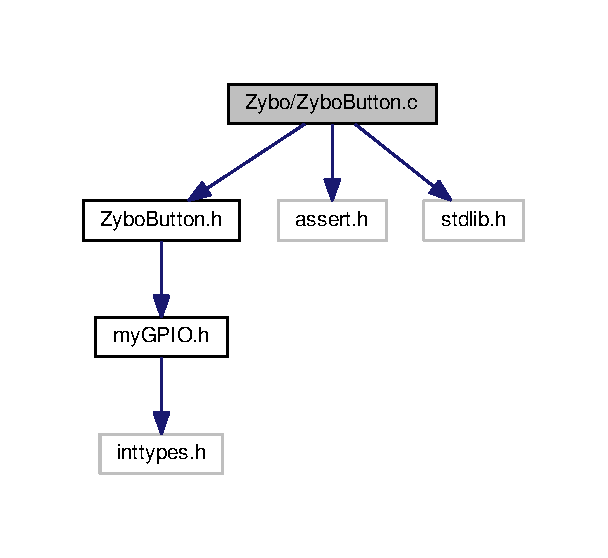
\includegraphics[width=292pt]{_zybo_button_8c__incl}
\end{center}
\end{figure}
\subsection*{Definizioni}
\begin{DoxyCompactItemize}
\item 
\#define \hyperlink{_zybo_button_8c_a5f45c877d1e8266f8a2c1d0b87746950}{timer\+\_\+wait\+\_\+ms}(ms)~usleep(ms$<$$<$10)
\end{DoxyCompactItemize}
\subsection*{Funzioni}
\begin{DoxyCompactItemize}
\item 
void \hyperlink{group___button_gaa40462223af93b0f5bdf2932400fe2a5}{Zybo\+Button\+\_\+init} (\hyperlink{struct_zybo_button__t}{Zybo\+Button\+\_\+t} $\ast$buttons, G\+P\+I\+O\+\_\+t $\ast$gpio, G\+P\+I\+O\+\_\+mask Button3\+\_\+pin, G\+P\+I\+O\+\_\+mask Button2\+\_\+pin, G\+P\+I\+O\+\_\+mask Button1\+\_\+pin, G\+P\+I\+O\+\_\+mask Button0\+\_\+pin)
\begin{DoxyCompactList}\small\item\em Inizializza un oggetto di tipo \hyperlink{struct_zybo_button__t}{Zybo\+Button\+\_\+t}. \end{DoxyCompactList}\item 
void \hyperlink{group___button_gaca30e81084e746785e395f79e9678e9a}{Zybo\+Button\+\_\+wait\+While\+Idle} (\hyperlink{struct_zybo_button__t}{Zybo\+Button\+\_\+t} $\ast$buttons)
\begin{DoxyCompactList}\small\item\em Permettere di mettere il programma in attesa attiva finche' i button restano inattivi;. \end{DoxyCompactList}\item 
void \hyperlink{group___button_ga3840edf011b5bad6302b7efc9c6326fe}{Zybo\+Button\+\_\+wait\+While\+Busy} (\hyperlink{struct_zybo_button__t}{Zybo\+Button\+\_\+t} $\ast$buttons)
\begin{DoxyCompactList}\small\item\em Permettere di mettere il programma in attesa attiva finche' i button restano attivi;. \end{DoxyCompactList}\item 
\hyperlink{group___button_ga85c290bfa232cab213e69200bf78e06a}{Zybo\+Button\+\_\+status\+\_\+t} \hyperlink{group___button_ga75407539e8ba0ad3ea142496219cd083}{Zybo\+Button\+\_\+get\+Status} (\hyperlink{struct_zybo_button__t}{Zybo\+Button\+\_\+t} $\ast$buttons, \hyperlink{group___button_ga4d26a5f6cad606de534ba034e0ba42dd}{Zybo\+Button\+\_\+mask\+\_\+t} mask)
\begin{DoxyCompactList}\small\item\em Permette la lettura dello stato dei button presenti sulla board. \end{DoxyCompactList}\end{DoxyCompactItemize}


\subsection{Documentazione delle definizioni}
\hypertarget{_zybo_button_8c_a5f45c877d1e8266f8a2c1d0b87746950}{\index{Zybo\+Button.\+c@{Zybo\+Button.\+c}!timer\+\_\+wait\+\_\+ms@{timer\+\_\+wait\+\_\+ms}}
\index{timer\+\_\+wait\+\_\+ms@{timer\+\_\+wait\+\_\+ms}!Zybo\+Button.\+c@{Zybo\+Button.\+c}}
\subsubsection[{timer\+\_\+wait\+\_\+ms}]{\setlength{\rightskip}{0pt plus 5cm}\#define timer\+\_\+wait\+\_\+ms(
\begin{DoxyParamCaption}
\item[{}]{ms}
\end{DoxyParamCaption}
)~usleep(ms$<$$<$10)}}\label{_zybo_button_8c_a5f45c877d1e8266f8a2c1d0b87746950}

\hypertarget{_zybo_button_8h}{\section{Riferimenti per il file Zybo/\+Zybo\+Button.h}
\label{_zybo_button_8h}\index{Zybo/\+Zybo\+Button.\+h@{Zybo/\+Zybo\+Button.\+h}}
}
{\ttfamily \#include \char`\"{}gpio.\+h\char`\"{}}\\*
Grafo delle dipendenze di inclusione per Zybo\+Button.\+h\+:\nopagebreak
\begin{figure}[H]
\begin{center}
\leavevmode
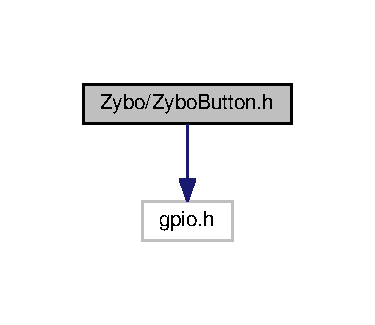
\includegraphics[width=180pt]{_zybo_button_8h__incl}
\end{center}
\end{figure}
Questo grafo mostra quali altri file includono direttamente o indirettamente questo file\+:\nopagebreak
\begin{figure}[H]
\begin{center}
\leavevmode
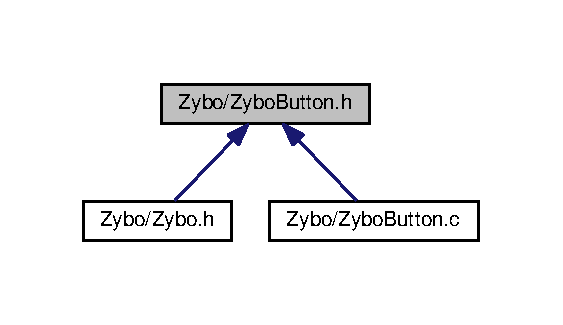
\includegraphics[width=270pt]{_zybo_button_8h__dep__incl}
\end{center}
\end{figure}
\subsection*{Strutture dati}
\begin{DoxyCompactItemize}
\item 
struct \hyperlink{struct_zybo_button__t}{Zybo\+Button\+\_\+t}
\begin{DoxyCompactList}\small\item\em Struttura opaca che astrae l'insieme dei button presenti sulla board Digilent Zybo;. \end{DoxyCompactList}\end{DoxyCompactItemize}
\subsection*{Definizioni}
\begin{DoxyCompactItemize}
\item 
\#define \hyperlink{group___button_ga5f85cbc14732f1d83faa75500b67defa}{Zybo\+Button}(i)~((uint32\+\_\+t)(1$<$$<$i))
\begin{DoxyCompactList}\small\item\em Metodo alternativo per la specifica di uno dei button presenti sulla board Digilent Zybo. \end{DoxyCompactList}\item 
\#define \hyperlink{group___button_ga8960eefa6a431f50d4fe2a2f8063da3f}{Zybo\+Button\+\_\+\+Debounce\+Wait}~50
\begin{DoxyCompactList}\small\item\em Tempo di attesa (in millisecondi) usato per prevenire il fenomeno del bouncing. Il valore di default è 50, determinato empiricamente. Puo' essere modificato a piacimento cambiando il valore alla macro seguente. \end{DoxyCompactList}\end{DoxyCompactItemize}
\subsection*{Tipi enumerati (enum)}
\begin{DoxyCompactItemize}
\item 
enum \hyperlink{group___button_ga4d26a5f6cad606de534ba034e0ba42dd}{Zybo\+Button\+\_\+mask\+\_\+t} \{ \hyperlink{group___button_gga4d26a5f6cad606de534ba034e0ba42ddaabede392be8cae14b8a070a804c754e8}{Zybo\+Button3} = 0x8, 
\hyperlink{group___button_gga4d26a5f6cad606de534ba034e0ba42dda2aa888c8f01ac8a79013e5ebc9eef609}{Zybo\+Button2} = 0x4, 
\hyperlink{group___button_gga4d26a5f6cad606de534ba034e0ba42dda29c35ef3133898c050f675a60de66dd7}{Zybo\+Button1} = 0x2, 
\hyperlink{group___button_gga4d26a5f6cad606de534ba034e0ba42dda2f821ce9661687aefb0ec4de65911570}{Zybo\+Button0} = 0x1
 \}
\begin{DoxyCompactList}\small\item\em Maschere di selezione dei Push\+Button. \end{DoxyCompactList}\item 
enum \hyperlink{group___button_ga85c290bfa232cab213e69200bf78e06a}{Zybo\+Button\+\_\+status\+\_\+t} \{ \hyperlink{group___button_gga85c290bfa232cab213e69200bf78e06aacd110f28912806bcec929721e8737399}{Zybo\+Button\+\_\+off}, 
\hyperlink{group___button_gga85c290bfa232cab213e69200bf78e06aa49bf4a6902270f28bc6a1146fbd1b1fe}{Zybo\+Button\+\_\+on}
 \}
\begin{DoxyCompactList}\small\item\em Status di attivo/inattivo dei Push\+Button. \end{DoxyCompactList}\end{DoxyCompactItemize}
\subsection*{Funzioni}
\begin{DoxyCompactItemize}
\item 
void \hyperlink{group___button_gaa40462223af93b0f5bdf2932400fe2a5}{Zybo\+Button\+\_\+init} (\hyperlink{struct_zybo_button__t}{Zybo\+Button\+\_\+t} $\ast$buttons, \hyperlink{struct_g_p_i_o__t}{G\+P\+I\+O\+\_\+t} $\ast$gpio, \hyperlink{group___g_p_i_o_ga6d5aef8a8a54ee2f602d47252ff66595}{G\+P\+I\+O\+\_\+mask} Button3\+\_\+pin, \hyperlink{group___g_p_i_o_ga6d5aef8a8a54ee2f602d47252ff66595}{G\+P\+I\+O\+\_\+mask} Button2\+\_\+pin, \hyperlink{group___g_p_i_o_ga6d5aef8a8a54ee2f602d47252ff66595}{G\+P\+I\+O\+\_\+mask} Button1\+\_\+pin, \hyperlink{group___g_p_i_o_ga6d5aef8a8a54ee2f602d47252ff66595}{G\+P\+I\+O\+\_\+mask} Button0\+\_\+pin)
\begin{DoxyCompactList}\small\item\em Inizializza un oggetto di tipo \hyperlink{struct_zybo_button__t}{Zybo\+Button\+\_\+t}. \end{DoxyCompactList}\item 
void \hyperlink{group___button_gaca30e81084e746785e395f79e9678e9a}{Zybo\+Button\+\_\+wait\+While\+Idle} (\hyperlink{struct_zybo_button__t}{Zybo\+Button\+\_\+t} $\ast$buttons)
\begin{DoxyCompactList}\small\item\em Permettere di mettere il programma in attesa attiva finche' i button restano inattivi;. \end{DoxyCompactList}\item 
void \hyperlink{group___button_ga3840edf011b5bad6302b7efc9c6326fe}{Zybo\+Button\+\_\+wait\+While\+Busy} (\hyperlink{struct_zybo_button__t}{Zybo\+Button\+\_\+t} $\ast$buttons)
\begin{DoxyCompactList}\small\item\em Permettere di mettere il programma in attesa attiva finche' i button restano attivi;. \end{DoxyCompactList}\item 
\hyperlink{group___button_ga85c290bfa232cab213e69200bf78e06a}{Zybo\+Button\+\_\+status\+\_\+t} \hyperlink{group___button_ga75407539e8ba0ad3ea142496219cd083}{Zybo\+Button\+\_\+get\+Status} (\hyperlink{struct_zybo_button__t}{Zybo\+Button\+\_\+t} $\ast$buttons, \hyperlink{group___button_ga4d26a5f6cad606de534ba034e0ba42dd}{Zybo\+Button\+\_\+mask\+\_\+t} mask)
\begin{DoxyCompactList}\small\item\em Permette la lettura dello stato dei button presenti sulla board. \end{DoxyCompactList}\end{DoxyCompactItemize}

\hypertarget{_zybo_led_8c}{\section{Riferimenti per il file Zybo/\+Zybo\+Led.c}
\label{_zybo_led_8c}\index{Zybo/\+Zybo\+Led.\+c@{Zybo/\+Zybo\+Led.\+c}}
}
{\ttfamily \#include \char`\"{}Zybo\+Led.\+h\char`\"{}}\\*
{\ttfamily \#include $<$assert.\+h$>$}\\*
{\ttfamily \#include $<$stdlib.\+h$>$}\\*
Grafo delle dipendenze di inclusione per Zybo\+Led.\+c\+:\nopagebreak
\begin{figure}[H]
\begin{center}
\leavevmode
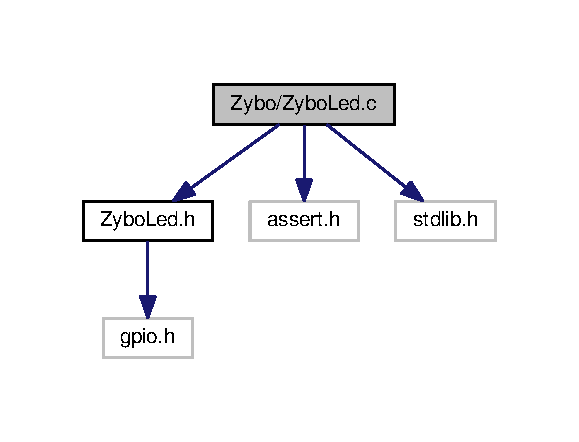
\includegraphics[width=279pt]{_zybo_led_8c__incl}
\end{center}
\end{figure}
\subsection*{Funzioni}
\begin{DoxyCompactItemize}
\item 
static int \hyperlink{_zybo_led_8c_a2a3452033228e251b3897e89a8ebcc7e}{validate\+Pair} (\hyperlink{struct_zybo_led__t}{Zybo\+Led\+\_\+t} $\ast$leds)
\item 
void \hyperlink{group___led_ga51bccd37e6ae8cd32e2c50c60a5e83cc}{Zybo\+Led\+\_\+init} (\hyperlink{struct_zybo_led__t}{Zybo\+Led\+\_\+t} $\ast$leds, \hyperlink{structmy_g_p_i_o__t}{my\+G\+P\+I\+O\+\_\+t} $\ast$gpio, \hyperlink{group__my_g_p_i_o_ga402a0d20afc0cb7c25554b8b023f4253}{my\+G\+P\+I\+O\+\_\+mask} Led3\+\_\+pin, \hyperlink{group__my_g_p_i_o_ga402a0d20afc0cb7c25554b8b023f4253}{my\+G\+P\+I\+O\+\_\+mask} Led2\+\_\+pin, \hyperlink{group__my_g_p_i_o_ga402a0d20afc0cb7c25554b8b023f4253}{my\+G\+P\+I\+O\+\_\+mask} Led1\+\_\+pin, \hyperlink{group__my_g_p_i_o_ga402a0d20afc0cb7c25554b8b023f4253}{my\+G\+P\+I\+O\+\_\+mask} Led0\+\_\+pin)
\begin{DoxyCompactList}\small\item\em Inizializza un oggetto di tipo \hyperlink{struct_zybo_led__t}{Zybo\+Led\+\_\+t}. \end{DoxyCompactList}\item 
void \hyperlink{group___led_gacf5c2b0328c4bdf2d796397fc4510c69}{Zybo\+Led\+\_\+set\+Status} (\hyperlink{struct_zybo_led__t}{Zybo\+Led\+\_\+t} $\ast$leds, \hyperlink{group___led_gad11701cccac394f7e1f90de8f85695f3}{Zybo\+Led\+\_\+mask\+\_\+t} mask, \hyperlink{group___led_ga3dcb274f22e577705c49944b8d1f4b12}{Zybo\+Led\+\_\+status\+\_\+t} status)
\begin{DoxyCompactList}\small\item\em Permette di accendere/spegnere i Led sulla board. \end{DoxyCompactList}\item 
void \hyperlink{group___led_ga20ddd78a98b4c0123c5b964aa0a59046}{Zybo\+Led\+\_\+toggle} (\hyperlink{struct_zybo_led__t}{Zybo\+Led\+\_\+t} $\ast$leds, \hyperlink{group___led_gad11701cccac394f7e1f90de8f85695f3}{Zybo\+Led\+\_\+mask\+\_\+t} mask)
\begin{DoxyCompactList}\small\item\em Permette di accendere/spegnere i Led sulla board, invertendone il valore. \end{DoxyCompactList}\end{DoxyCompactItemize}


\subsection{Descrizione dettagliata}
\begin{DoxyAuthor}{Autore}
Salvatore Barone \href{mailto:salvator.barone@gmail.com}{\tt salvator.\+barone@gmail.\+com}
\end{DoxyAuthor}
\begin{DoxyCopyright}{Copyright}
Copyright 2017 Salvatore Barone \href{mailto:salvator.barone@gmail.com}{\tt salvator.\+barone@gmail.\+com}
\end{DoxyCopyright}
This file is part of Zynq7000\+Driver\+Pack

Zynq7000\+Driver\+Pack is free software; you can redistribute it and/or modify it under the terms of the G\+N\+U General Public License as published by the Free Software Foundation; either version 3 of the License, or any later version.

Zynq7000\+Driver\+Pack is distributed in the hope that it will be useful, but W\+I\+T\+H\+O\+U\+T A\+N\+Y W\+A\+R\+R\+A\+N\+T\+Y; without even the implied warranty of M\+E\+R\+C\+H\+A\+N\+T\+A\+B\+I\+L\+I\+T\+Y or F\+I\+T\+N\+E\+S\+S F\+O\+R A P\+A\+R\+T\+I\+C\+U\+L\+A\+R P\+U\+R\+P\+O\+S\+E. See the G\+N\+U General Public License for more details.

You should have received a copy of the G\+N\+U General Public License along with this program; if not, write to the Free Software Foundation, Inc., 51 Franklin Street, Fifth Floor, Boston, M\+A 02110-\/1301, U\+S\+A. 

\subsection{Documentazione delle funzioni}
\hypertarget{_zybo_led_8c_a2a3452033228e251b3897e89a8ebcc7e}{\index{Zybo\+Led.\+c@{Zybo\+Led.\+c}!validate\+Pair@{validate\+Pair}}
\index{validate\+Pair@{validate\+Pair}!Zybo\+Led.\+c@{Zybo\+Led.\+c}}
\subsubsection[{validate\+Pair}]{\setlength{\rightskip}{0pt plus 5cm}static int validate\+Pair (
\begin{DoxyParamCaption}
\item[{{\bf Zybo\+Led\+\_\+t} $\ast$}]{leds}
\end{DoxyParamCaption}
)\hspace{0.3cm}{\ttfamily [static]}}}\label{_zybo_led_8c_a2a3452033228e251b3897e89a8ebcc7e}

\hypertarget{_zybo_led_8h}{\section{Riferimenti per il file Zybo/\+Zybo\+Led.h}
\label{_zybo_led_8h}\index{Zybo/\+Zybo\+Led.\+h@{Zybo/\+Zybo\+Led.\+h}}
}
{\ttfamily \#include \char`\"{}my\+G\+P\+I\+O.\+h\char`\"{}}\\*
Grafo delle dipendenze di inclusione per Zybo\+Led.\+h\+:\nopagebreak
\begin{figure}[H]
\begin{center}
\leavevmode
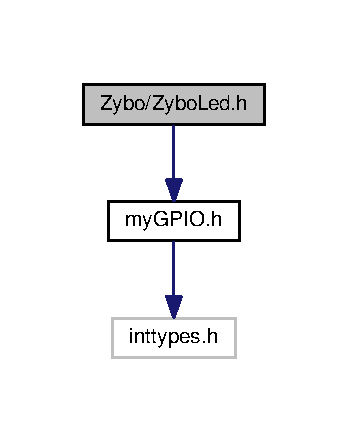
\includegraphics[width=167pt]{_zybo_led_8h__incl}
\end{center}
\end{figure}
Questo grafo mostra quali altri file includono direttamente o indirettamente questo file\+:\nopagebreak
\begin{figure}[H]
\begin{center}
\leavevmode
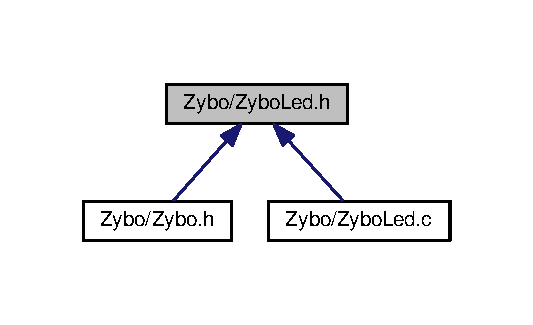
\includegraphics[width=256pt]{_zybo_led_8h__dep__incl}
\end{center}
\end{figure}
\subsection*{Strutture dati}
\begin{DoxyCompactItemize}
\item 
struct \hyperlink{struct_zybo_led__t}{Zybo\+Led\+\_\+t}
\begin{DoxyCompactList}\small\item\em Struttura opaca che astrae l'insieme dei Led presenti sulla board Digilent Zybo;. \end{DoxyCompactList}\end{DoxyCompactItemize}
\subsection*{Definizioni}
\begin{DoxyCompactItemize}
\item 
\#define \hyperlink{group___led_ga50ab39fed34dc3aaf53cdfd67d8ba25d}{Zybo\+Led}(i)~((uint32\+\_\+t)(1$<$$<$(i)))
\begin{DoxyCompactList}\small\item\em Metodo alternativo per la specifica di uno dei led presenti sulla board Digilent Zybo. \end{DoxyCompactList}\end{DoxyCompactItemize}
\subsection*{Tipi enumerati (enum)}
\begin{DoxyCompactItemize}
\item 
enum \hyperlink{group___led_gad11701cccac394f7e1f90de8f85695f3}{Zybo\+Led\+\_\+mask\+\_\+t} \{ \hyperlink{group___led_ggad11701cccac394f7e1f90de8f85695f3adc5edc2adfd899da9f149cb61364b141}{Zybo\+Led3} = 0x8\+U, 
\hyperlink{group___led_ggad11701cccac394f7e1f90de8f85695f3a4fa521f6fce7c4ba77d1d8144e71cdfc}{Zybo\+Led2} = 0x4\+U, 
\hyperlink{group___led_ggad11701cccac394f7e1f90de8f85695f3ad71c06f65dfffcf825d48f287718d9be}{Zybo\+Led1} = 0x2\+U, 
\hyperlink{group___led_ggad11701cccac394f7e1f90de8f85695f3ae1a1e8fa0bf803793ff27004884b85fe}{Zybo\+Led0} = 0x1\+U
 \}
\begin{DoxyCompactList}\small\item\em Maschere di selezione dei led. \end{DoxyCompactList}\item 
enum \hyperlink{group___led_ga3dcb274f22e577705c49944b8d1f4b12}{Zybo\+Led\+\_\+status\+\_\+t} \{ \hyperlink{group___led_gga3dcb274f22e577705c49944b8d1f4b12a9679f1c302afdb51915a2331b4ec92f3}{Zybo\+Led\+\_\+off}, 
\hyperlink{group___led_gga3dcb274f22e577705c49944b8d1f4b12aafcf0ae16a6edec807c06bb0a99f7e8b}{Zybo\+Led\+\_\+on}
 \}
\begin{DoxyCompactList}\small\item\em Status di accensione/spegnimento dei led. \end{DoxyCompactList}\end{DoxyCompactItemize}
\subsection*{Funzioni}
\begin{DoxyCompactItemize}
\item 
void \hyperlink{group___led_ga51bccd37e6ae8cd32e2c50c60a5e83cc}{Zybo\+Led\+\_\+init} (\hyperlink{struct_zybo_led__t}{Zybo\+Led\+\_\+t} $\ast$leds, \hyperlink{structmy_g_p_i_o__t}{my\+G\+P\+I\+O\+\_\+t} $\ast$gpio, \hyperlink{group__my_g_p_i_o_ga402a0d20afc0cb7c25554b8b023f4253}{my\+G\+P\+I\+O\+\_\+mask} Led3\+\_\+pin, \hyperlink{group__my_g_p_i_o_ga402a0d20afc0cb7c25554b8b023f4253}{my\+G\+P\+I\+O\+\_\+mask} Led2\+\_\+pin, \hyperlink{group__my_g_p_i_o_ga402a0d20afc0cb7c25554b8b023f4253}{my\+G\+P\+I\+O\+\_\+mask} Led1\+\_\+pin, \hyperlink{group__my_g_p_i_o_ga402a0d20afc0cb7c25554b8b023f4253}{my\+G\+P\+I\+O\+\_\+mask} Led0\+\_\+pin)
\begin{DoxyCompactList}\small\item\em Inizializza un oggetto di tipo \hyperlink{struct_zybo_led__t}{Zybo\+Led\+\_\+t}. \end{DoxyCompactList}\item 
void \hyperlink{group___led_gacf5c2b0328c4bdf2d796397fc4510c69}{Zybo\+Led\+\_\+set\+Status} (\hyperlink{struct_zybo_led__t}{Zybo\+Led\+\_\+t} $\ast$leds, \hyperlink{group___led_gad11701cccac394f7e1f90de8f85695f3}{Zybo\+Led\+\_\+mask\+\_\+t} mask, \hyperlink{group___led_ga3dcb274f22e577705c49944b8d1f4b12}{Zybo\+Led\+\_\+status\+\_\+t} status)
\begin{DoxyCompactList}\small\item\em Permette di accendere/spegnere i Led sulla board. \end{DoxyCompactList}\item 
void \hyperlink{group___led_ga20ddd78a98b4c0123c5b964aa0a59046}{Zybo\+Led\+\_\+toggle} (\hyperlink{struct_zybo_led__t}{Zybo\+Led\+\_\+t} $\ast$leds, \hyperlink{group___led_gad11701cccac394f7e1f90de8f85695f3}{Zybo\+Led\+\_\+mask\+\_\+t} mask)
\begin{DoxyCompactList}\small\item\em Permette di accendere/spegnere i Led sulla board, invertendone il valore. \end{DoxyCompactList}\end{DoxyCompactItemize}


\subsection{Descrizione dettagliata}
\begin{DoxyAuthor}{Autore}
Salvatore Barone \href{mailto:salvator.barone@gmail.com}{\tt salvator.\+barone@gmail.\+com}
\end{DoxyAuthor}
\begin{DoxyCopyright}{Copyright}
Copyright 2017 Salvatore Barone \href{mailto:salvator.barone@gmail.com}{\tt salvator.\+barone@gmail.\+com}
\end{DoxyCopyright}
This file is part of Zynq7000\+Driver\+Pack

Zynq7000\+Driver\+Pack is free software; you can redistribute it and/or modify it under the terms of the G\+N\+U General Public License as published by the Free Software Foundation; either version 3 of the License, or any later version.

Zynq7000\+Driver\+Pack is distributed in the hope that it will be useful, but W\+I\+T\+H\+O\+U\+T A\+N\+Y W\+A\+R\+R\+A\+N\+T\+Y; without even the implied warranty of M\+E\+R\+C\+H\+A\+N\+T\+A\+B\+I\+L\+I\+T\+Y or F\+I\+T\+N\+E\+S\+S F\+O\+R A P\+A\+R\+T\+I\+C\+U\+L\+A\+R P\+U\+R\+P\+O\+S\+E. See the G\+N\+U General Public License for more details.

You should have received a copy of the G\+N\+U General Public License along with this program; if not, write to the Free Software Foundation, Inc., 51 Franklin Street, Fifth Floor, Boston, M\+A 02110-\/1301, U\+S\+A. 
\hypertarget{_zybo_switch_8c}{\section{Riferimenti per il file Zybo/\+Zybo\+Switch.c}
\label{_zybo_switch_8c}\index{Zybo/\+Zybo\+Switch.\+c@{Zybo/\+Zybo\+Switch.\+c}}
}
{\ttfamily \#include \char`\"{}Zybo\+Switch.\+h\char`\"{}}\\*
{\ttfamily \#include $<$assert.\+h$>$}\\*
{\ttfamily \#include $<$stdlib.\+h$>$}\\*
Grafo delle dipendenze di inclusione per Zybo\+Switch.\+c\+:\nopagebreak
\begin{figure}[H]
\begin{center}
\leavevmode
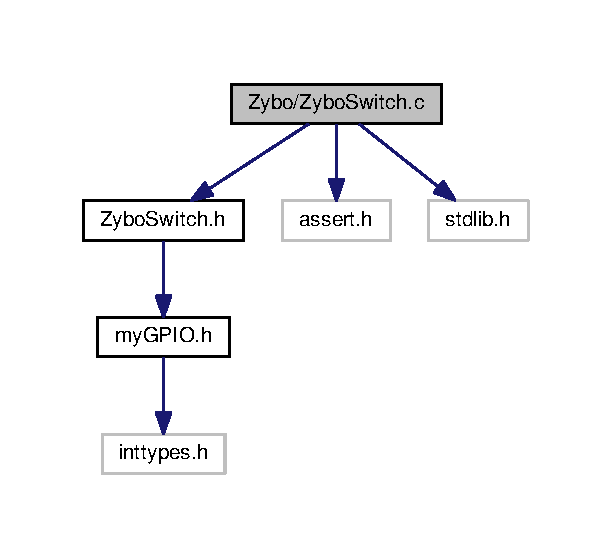
\includegraphics[width=294pt]{_zybo_switch_8c__incl}
\end{center}
\end{figure}
\subsection*{Funzioni}
\begin{DoxyCompactItemize}
\item 
void \hyperlink{group___switch_ga121018c0ccfeb05b6e8f692a5a6955d7}{Zybo\+Switch\+\_\+init} (\hyperlink{struct_zybo_switch__t}{Zybo\+Switch\+\_\+t} $\ast$switches, \hyperlink{struct_g_p_i_o__t}{G\+P\+I\+O\+\_\+t} $\ast$gpio, \hyperlink{group___g_p_i_o_ga6d5aef8a8a54ee2f602d47252ff66595}{G\+P\+I\+O\+\_\+mask} Switch3\+\_\+pin, \hyperlink{group___g_p_i_o_ga6d5aef8a8a54ee2f602d47252ff66595}{G\+P\+I\+O\+\_\+mask} Switch2\+\_\+pin, \hyperlink{group___g_p_i_o_ga6d5aef8a8a54ee2f602d47252ff66595}{G\+P\+I\+O\+\_\+mask} Switch1\+\_\+pin, \hyperlink{group___g_p_i_o_ga6d5aef8a8a54ee2f602d47252ff66595}{G\+P\+I\+O\+\_\+mask} Switch0\+\_\+pin)
\begin{DoxyCompactList}\small\item\em Inizializza un oggetto di tipo \hyperlink{struct_zybo_switch__t}{Zybo\+Switch\+\_\+t}. \end{DoxyCompactList}\item 
\hyperlink{group___switch_ga4ba6b49b2f47ebb464aefcea7e23e04a}{Zybo\+Switch\+\_\+status\+\_\+t} \hyperlink{group___switch_gafac8daf9a9a585f8f20ef2a6fa883a1f}{Zybo\+Switch\+\_\+get\+Status} (\hyperlink{struct_zybo_switch__t}{Zybo\+Switch\+\_\+t} $\ast$switches, \hyperlink{group___switch_ga2e0602a824354f25c395f938caba3703}{Zybo\+Switch\+\_\+mask\+\_\+t} mask)
\begin{DoxyCompactList}\small\item\em Permette la lettura dello stato degli switch presenti sulla board. \end{DoxyCompactList}\end{DoxyCompactItemize}

\hypertarget{_zybo_switch_8h}{\section{Riferimenti per il file Zybo/\+Zybo\+Switch.h}
\label{_zybo_switch_8h}\index{Zybo/\+Zybo\+Switch.\+h@{Zybo/\+Zybo\+Switch.\+h}}
}
{\ttfamily \#include \char`\"{}gpio.\+h\char`\"{}}\\*
Grafo delle dipendenze di inclusione per Zybo\+Switch.\+h\+:
\nopagebreak
\begin{figure}[H]
\begin{center}
\leavevmode
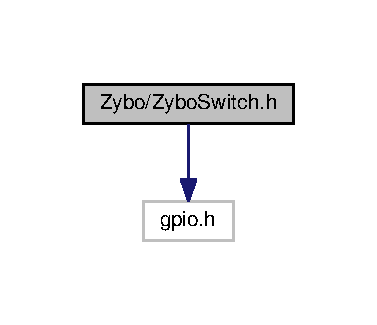
\includegraphics[width=181pt]{_zybo_switch_8h__incl}
\end{center}
\end{figure}
Questo grafo mostra quali altri file includono direttamente o indirettamente questo file\+:
\nopagebreak
\begin{figure}[H]
\begin{center}
\leavevmode
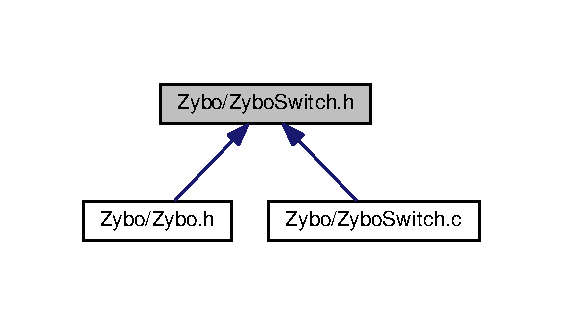
\includegraphics[width=270pt]{_zybo_switch_8h__dep__incl}
\end{center}
\end{figure}
\subsection*{Strutture dati}
\begin{DoxyCompactItemize}
\item 
struct \hyperlink{struct_zybo_switch__t}{Zybo\+Switch\+\_\+t}
\begin{DoxyCompactList}\small\item\em Struttura opaca che astrae l'insieme degli switch presenti sulla board Digilent Zybo;. \end{DoxyCompactList}\end{DoxyCompactItemize}
\subsection*{Definizioni}
\begin{DoxyCompactItemize}
\item 
\#define \hyperlink{group___switch_ga1c463f6e1e3a43f68109c176772ce5cc}{Zybo\+Switch}(i)~((uint32\+\_\+t)(1$<$$<$i))
\begin{DoxyCompactList}\small\item\em Metodo alternativo per la specifica di uno degli switch presenti sulla board Digilent Zybo. \end{DoxyCompactList}\end{DoxyCompactItemize}
\subsection*{Tipi enumerati (enum)}
\begin{DoxyCompactItemize}
\item 
enum \hyperlink{group___switch_ga2e0602a824354f25c395f938caba3703}{Zybo\+Switch\+\_\+mask\+\_\+t} \{ \hyperlink{group___switch_gga2e0602a824354f25c395f938caba3703a73ccea5ad8c919fe962e9a67a3733ee3}{Zybo\+Switch3} = 0x8\+U, 
\hyperlink{group___switch_gga2e0602a824354f25c395f938caba3703aac2f5ebb28eb3bd93fcdf8019b6a3e9e}{Zybo\+Switch2} = 0x4\+U, 
\hyperlink{group___switch_gga2e0602a824354f25c395f938caba3703a694a25c87b1ec597d2a6032bf5d34b0f}{Zybo\+Switch1} = 0x2\+U, 
\hyperlink{group___switch_gga2e0602a824354f25c395f938caba3703a84350e8b6e7a7e2cabf22fc7a1a5c651}{Zybo\+Switch0} = 0x1\+U
 \}
\begin{DoxyCompactList}\small\item\em Maschere di selezione degli switch. \end{DoxyCompactList}\item 
enum \hyperlink{group___switch_ga4ba6b49b2f47ebb464aefcea7e23e04a}{Zybo\+Switch\+\_\+status\+\_\+t} \{ \hyperlink{group___switch_gga4ba6b49b2f47ebb464aefcea7e23e04aa1d686faf83e8606e68eec0b7e525a755}{Zybo\+Switch\+\_\+off}, 
\hyperlink{group___switch_gga4ba6b49b2f47ebb464aefcea7e23e04aafba009508b8822de867af69034e3e4f8}{Zybo\+Switch\+\_\+on}
 \}
\begin{DoxyCompactList}\small\item\em Status di attivo/inattivo degli switch. \end{DoxyCompactList}\end{DoxyCompactItemize}
\subsection*{Funzioni}
\begin{DoxyCompactItemize}
\item 
void \hyperlink{group___switch_ga121018c0ccfeb05b6e8f692a5a6955d7}{Zybo\+Switch\+\_\+init} (\hyperlink{struct_zybo_switch__t}{Zybo\+Switch\+\_\+t} $\ast$switches, G\+P\+I\+O\+\_\+t $\ast$gpio, G\+P\+I\+O\+\_\+mask Switch3\+\_\+pin, G\+P\+I\+O\+\_\+mask Switch2\+\_\+pin, G\+P\+I\+O\+\_\+mask Switch1\+\_\+pin, G\+P\+I\+O\+\_\+mask Switch0\+\_\+pin)
\begin{DoxyCompactList}\small\item\em Inizializza un oggetto di tipo \hyperlink{struct_zybo_switch__t}{Zybo\+Switch\+\_\+t}. \end{DoxyCompactList}\item 
\hyperlink{group___switch_ga4ba6b49b2f47ebb464aefcea7e23e04a}{Zybo\+Switch\+\_\+status\+\_\+t} \hyperlink{group___switch_gafac8daf9a9a585f8f20ef2a6fa883a1f}{Zybo\+Switch\+\_\+get\+Status} (\hyperlink{struct_zybo_switch__t}{Zybo\+Switch\+\_\+t} $\ast$switches, \hyperlink{group___switch_ga2e0602a824354f25c395f938caba3703}{Zybo\+Switch\+\_\+mask\+\_\+t} mask)
\begin{DoxyCompactList}\small\item\em Permette la lettura dello stato degli switch presenti sulla board. \end{DoxyCompactList}\end{DoxyCompactItemize}

%--- End generated contents ---

% Index
\newpage
\phantomsection
\addcontentsline{toc}{chapter}{Indice}
\printindex

\end{document}
